\documentclass[a4paper, twoside, openright]{memoir}
%      ^^ set here if oneside/twoside

\usepackage[english]{babel}

\usepackage[OT1]{fontenc}
\usepackage[utf8]{inputenc}



\usepackage[
    top=3cm, bottom=3cm,
    textwidth=13cm,
    bindingoffset=0cm,includemp,
    inner=2.5cm,  % only if twosided
    %% configure margin notes
    marginparsep=7mm, marginparwidth=3.5cm,
    marginparsep=5mm,
    %% reverse side of marginpar
    %reversemp,   
    ]{geometry}

% load everything else from class mymemoir
% =============================================================
%   LaTeX memoir template    ----------------------------------
%   ver 1.0 //  major review 1.0  //  January 2023, 10th
%
%   by Francesco Barone, github.com/baronefr
%   limited access CC licence (temporarily)
% -------------------------------------------------------------
%  some geometry components have been adapted from
%       [feth-zurich-cadmo-thesis-template-v2]
% -------------------------------------------------------------


% ============================
%   REQUIREMENTS
% ============================

% this packages have been moved to main.tex

% \usepackage[english]{babel}
% \usepackage[OT1]{fontenc}
% \usepackage[utf8]{inputenc}

% \usepackage{geometry}   
%     ref: https://texdoc.org/serve/geometry.pdf/0
%
%   [ info ] recommended geometry -----
%      top=3cm, bottom=3cm,
%      twoside, inner=2.5cm,
%      textwidth=13cm,
%      marginparsep=.7cm, marginparwidth=3.5cm
%
% further optional customizations might include
% \linespread{1.5}


\usepackage{fancyhdr}
\usepackage{authblk}

%\usepackage[sc]{mathpazo}  % to use palatino (if you like it)
\usepackage{amsmath,amssymb,amsfonts,mathrsfs}
\usepackage{mathalpha}
\usepackage{mathtools}
\usepackage{physics}
\usepackage[makeroom]{cancel}

\usepackage{graphicx}
\usepackage[most]{tcolorbox}
%\usepackage{marginnote}
\usepackage[colorinlistoftodos, tickmarkheight=0.2cm, bordercolor=white, figcolor=white]{todonotes}
% ref: http://tug.ctan.org/macros/latex/contrib/todonotes/todonotes.pdf
\usepackage{marginnote}
%\newcommand{\marginnote}{\marginpar}
\usepackage{soul}

\usepackage{tikz}
\usepackage[caption=false]{subfig}
\usepackage{wrapfig}
\usepackage[margin=25pt, font=small, labelfont=bf, labelsep=quad]{caption}

\usepackage[absolute]{textpos}
\usepackage{emptypage}
\usepackage{rotating}

\usepackage{multirow}
\usepackage{multicol}
\usepackage{array}
\usepackage{tabularx}
\usepackage{floatflt}
\usepackage{float}
\usepackage{booktabs}

\usepackage[]{hyperref}



% ============================
%   DEFINITIONS
% ============================


%  COLORS -----------------------------------

% institutional colors
\definecolor{unipdRedPantano}{RGB}{155,0,20}
\definecolor{unipdRedPantanoDarker}{RGB}{125,0,20}
\definecolor{cernBlue}{RGB}{0,51,160}

% routine colors
\definecolor{myGreen}{RGB}{19, 171, 2}
\definecolor{myBlue}{RGB}{0,51,160}
\definecolor{myCyan}{rgb}{0.2, 0.6, 1}
\definecolor{myYellow}{RGB}{255, 187, 0}
\definecolor{myPurple}{RGB}{255, 0, 153}
\definecolor{myLightGrey}{RGB}{52,55,60}






% ============================
%   LAYOUT
% ============================

% set link colors
\hypersetup{
    colorlinks=true,
    urlcolor=unipdRedPantano,
    linkcolor=unipdRedPantanoDarker
}

% misc
\setlength{\beforechapskip}{0pt}
\renewcommand\Authands{ and }
\makeatletter
\let\authorlist\@author
\makeatother

\newcommand{\printauthorlist}{{%
  \expandafter\let\csname textsuperscript \endcsname\@gobble% Remove \textsuperscript 
  \AB@authlist}% Print list
}

% fixes ----------------------
\makeatletter
\if@twoside%
   %%% put the stuff for true here (twoside=true)
   %\newcommand\side{stuff for twoside}
\else%
   %\geometry{includemp}
\fi%  
\makeatother


%  CHAPTER STYLE -------------
\makeatletter
\makechapterstyle{mymadsen}{%
    \chapterstyle{madsen}
    \renewcommand*{\chapnumfont}{\chapnamefont}%
    \renewcommand*{\chaptitlefont}{\normalfont\HUGE\bfseries}%
}
\chapterstyle{mymadsen}

% if you wish to use a std chapter style, use these
%\chapterstyle{mych}
%\chapterstyle{madsen}
%\chapterstyle{veelo}
%\chapterstyle{companion}
%\chapterstyle{ell}


\setsecheadstyle{\Large\bfseries\sffamily}
\setsubsecheadstyle{\large\bfseries\sffamily}
\setsubsubsecheadstyle{\bfseries\sffamily}
\setparaheadstyle{\normalsize\bfseries\sffamily}
\setsubparaheadstyle{\normalsize\itshape\sffamily}
\setsubparaindent{0pt} % disable indent


%  HEAD/FOOT STYLE -----------
% fix margins of header
\newlength{\extendmargin}
\setlength{\extendmargin}{\marginparwidth + \marginparsep}

\newcommand{\setlayout}{

\pagestyle{fancy}
\fancyheadoffset[leh,roh]{\extendmargin}
\fancyfootoffset[leh,roh]{\extendmargin}
\renewcommand{\headrulewidth}{1pt}


\fancyhead{}
\fancyhead[RO]{\rightmark}
\if@twoside%
   \fancyhead[LE]{\textsc{\leftmark}}
\fi%  


\fancyfoot{}
%  (optional) make page number at outer margin
%\fancyfoot[LE,RO]{\thepage}  
%  otherwise: center
\fancyfoot[C]{\thepage}
\fancyfoot[L]{}
\fancyfoot[R]{}
}
\setlayout

% fix first page of each chapter to have same pagestyle without upper rule
\fancypagestyle{plain}{
    % use same style in chapter first page
    \pagestyle{fancy}
    \renewcommand{\headrulewidth}{0pt}
}






% ============================
%   SPECIAL PAGES
% ============================

\def\docuver{none}

\def\prependtitle{}
\def\appendtitle{}
\def\coverfoot{}
\def\coverlogo{}

\def\copyrightmention{}
\def\copyrightnotes{}

%  COVER PAGE ----------------


% Q:  should this be wrapped by
%     \begin{titlingpage}  ?
\makeatletter
\newcommand*{\firstpage}{%
\begingroup
\renewcommand{\thanks}[1]{} % remove thanks in first page
\parbox[b][0.95\textheight][t]{2cm}{
\raggedleft
\begin{turn}{90}
\begin{tikzpicture}[opacity=1]
    \node{\includegraphics[height=2cm]{\coverlogo}};
\end{tikzpicture}
\end{turn}
}
\hspace*{2ex}
\textcolor{coverline}{\rule{2pt}{0.95\textheight}}
\hspace*{5ex}
\parbox[b][0.95\textheight][t]{0.8\textwidth}{
    {\raggedright
        {\prependtitle\par}
        {\HUGE\sffamily\bfseries\@title\par}
        {\appendtitle\par}
        \vspace{2cm}
        {\Large\bfseries\@date\par}
    }
    \vfill
    {\large\bfseries\@author}\\
    
    \vspace{1cm}
    \coverfoot
    \vspace{1cm}
}
\thispagestyle{empty}
%\if@openright\cleardoublepage\else\clearpage\fi
\endgroup}
\makeatother

\renewcommand{\thanks}[1]{\footnote{\href{mailto:#1}{#1}}}

%  SECOND PAGE ---------------
\def\secondpage{\clearpage\null\vfill
%\let\thanks\footnote % list authors mail here
\pagestyle{empty}
\begin{minipage}[b]{0.9\textwidth}
\footnotesize\raggedright
\setlength{\parskip}{0.5\baselineskip}
\hrule
\vspace{.7cm}
Document written in \LaTeX.\par

\begin{minipage}{0.9\textwidth}
    \let\footnoterule\relax % omit footnote rule here (for thanks command)
    \textbf{\LaTeX\space template Copyright} \copyright 2022--\the\year\ Francesco Pio Barone (\href{https://github.com/baronefr}{GitHub@baronefr}). This attribution shall not be removed even if the template is used in other documents.\par
    \copyrightmention
\end{minipage}

\vspace{.7cm}
\copyrightnotes
\vspace{.7cm}

Document compiled on \today. \textbf{Version signature \docuver}.
\vspace{.7cm}

\hrule

\begin{center}
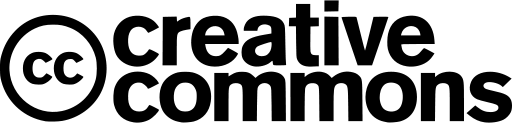
\includegraphics[height=.8cm]{style/cc.png}\hspace{1cm}

\includegraphics[height=.8cm]{style/ccmark.png}
\end{center}

This document is released under 
\textbf{Attribution-NonCommercial-ShareAlike 4.0 International} (\href{https://creativecommons.org/licenses/by-nc-sa/4.0/}{CC BY-NC-SA 4.0}) licence.

You are free to
\begin{itemize}
    \item Share — copy and redistribute the material in any medium or format
    \item Adapt — remix, transform, and build upon the material 
\end{itemize}

under the following terms:
\begin{itemize}
    \item Attribution — You must give appropriate credit, provide a link to the license, and indicate if changes were made. You may do so in any reasonable manner, but not in any way that suggests the licensor endorses you or your use.

    \item NonCommercial — You may not use the material for commercial purposes.

    \item ShareAlike — If you remix, transform, or build upon the material, you must distribute your contributions under the same license as the original.

    \item No additional restrictions — You may not apply legal terms or technological measures that legally restrict others from doing anything the license permits.
\end{itemize}
\end{minipage}
\vspace*{2\baselineskip}
\cleardoublepage
\rfoot{\thepage}}

% if you want to use second page with std \maketitle
\makeatletter
%\g@addto@macro{\maketitle}{\firstpage}
\g@addto@macro{\maketitle}{\secondpage}
\makeatother













% ============================
%   COMPONENTS
% ============================
\def\coverlogo{}
\def\copyrightnotes{}
\def\copyrightmention{}
\def\docuver{no-ver}
\def\prependtitle{}
\def\appendtitle{}
\def\coverfoot{}

% todo commands
%\newcommand{\todomark}{{\footnotesize\textbf{TODO} }}
\newcommand{\todomark}{\textbf{!} }
\newcommand{\todowarning}[2][]
    {\todo[color=yellow,bordercolor=white, #1]
     {\todomark #2}}
\newcommand{\todocritical}[2][]
    {\todo[color=red, bordercolor=white, textcolor=black,#1]
     {\todomark #2}}
\newcommand{\todogreen}[2][]
    {\todo[color=green,bordercolor=white, #1]
     {\todomark #2}}
\newcommand{\todoblue}[2][]
    {\todo[color=myBlue,bordercolor=white, textcolor=white, #1]
     {\todomark #2}}
\newcommand{\todocyan}[2][]
    {\todo[color=myCyan,bordercolor=white, #1]
     {\todomark #2}}


\makeatletter
\if@todonotes@disabled
    \newcommand{\todohl}[3][]{#2}
\else
    \newcommand{\todohl}[3][]{\hl{#2}\todo[color=yellow, backgroundcolor=white,bordercolor=yellow,#1]{\todomark #3}}
\fi
\makeatother

% margin boxes
\newcommand{\marginbox}[2][]
    {\todo[nolist, color=black, bordercolor=black, backgroundcolor=white, #1]{#2}}
\newcommand{\marginboxRed}[2][]
    {\todo[nolist,color=red!70, bordercolor=white, #1]{#2}}
\newcommand{\marginboxYellow}[2][]
    {\todo[nolist,color=myYellow,bordercolor=white, #1]{#2}}
\newcommand{\marginboxCyan}[2][]
    {\todo[nolist,color=myCyan,bordercolor=white, #1]{#2}}
\newcommand{\marginboxhl}[3][]{\hl{#2}\todo[nolist,color=yellow, backgroundcolor=white,bordercolor=yellow,#1]{#3}}

\newcommand{\marginbold}[1]{\marginnote{\textbf{#1}}}

\newcommand{\margintt}[1]{\marginnote{\texttt{#1}}}

\newcommand{\marginsf}
[1]{\marginnote{\sffamily#1}}


\newenvironment{enbox}[2][]{
\begin{tcolorbox}[breakable, enhanced, #1]
\textbf{#2}
}{
\end{tcolorbox}
}




\newcommand{\lecture}
[2][none]{
\marginnote{\textit{Lecture #2}}
}
\usepackage{bigints}
\usepackage{makecell}
\usepackage[bb=boondox]{mathalfa}
\usepackage{dsfont}
\usepackage[makeroom]{cancel}
\usepackage{amsmath}
\usepackage{witharrows} % look this ans: https://tex.stackexchange.com/questions/12621/multi-line-equations-with-explanations-on-some-lines

\newcolumntype{L}{>{\raggedright\arraybackslash}X}
\renewcommand{\appendixname}{}%
\newcommand{\parallelslant}{\mathbin{\!/\mkern-5mu/\!}}
\headsep = 30pt

\newcommand{\equalexpl}[1]{%
  \underset{\substack{\uparrow\\\mathrlap{\text{\hspace{-1em}#1}}}}{=}}


%\pagestyle{fancy}




% optional dependencies ----------
\usetikzlibrary{quantikz}
\usepackage{wasysym}
\usepackage{enumitem}
\usepackage{booktabs}
\usepackage{xcolor}
\usepackage{makecell}
\usepackage{blindtext}
\usepackage{arydshln}
\usepackage[normalem]{ulem}
\useunder{\uline}{\ul}{}
\usepackage{subfig}
\usepackage{lipsum}
\usepackage{mathalpha}
\usepackage{bbold}
\setcounter{secnumdepth}{2}
\setcounter{tocdepth}{2}

%\setlength{\parindent}{0pt}
\definecolor{coverline}{RGB}{205,0,20}

% --------------------------------
%             metadata
% --------------------------------

% version of the document
\def\docuver{DEV-117-rev3-handout-github}

\def\prependtitle{\LARGE{Notes of}}

\title{Quantum information with atoms and photons}

\def\appendtitle{ \vspace{3.0cm}
    \LARGE{Prof. Pietro Silvi\\
           Prof. Marco Di Liberto}
}

\def\coverfoot{Department of Physics and Astronomy, University of Padua}

\author{Ilaria Delbono\thanks{ilaria.delbono@studenti.unipd.it},
    Anna Garbo\thanks{anna.garbo.2@studenti.unipd.it},
    Giacomo Di Prima\thanks{giacomo.diprima@studenti.unipd.it},
    Davide Bacilieri\thanks{davide.bacilieri@studenti.unipd.it},
    Lorenzo Barbiero\thanks{lorenzo.barbiero.1@studenti.unipd.it},
    Francesco Pio Barone\thanks{francescopio.barone@studenti.unipd.it},
    Giosuè Sardo Infirri\thanks{giosue.sardoinfirri@studenti.unipd.it}
    and Lorenzo Valentini\thanks{lorenzo.valentini.2@studenti.unipd.it}
}


\date{Academic Year 2022/2023}

\def\coverlogo{style/unipd_logo_red.png}

\def\copyrightmention{
\textbf{Document content Copyright} 2022-\the\year\ to all the students mentioned in first page and hereby reported:
\authorlist.\\

To fix errors or to improve this document, contact Ilaria Delbono or Francesco Pio Barone.
}

\def\copyrightnotes{
The information included in this document has been verified at the best of the authors' knowledge. No responsibility will be attributed to the authors involved in their creation, publication and distribution. The Professors have not directly checked the content of this document, errors might be present!

Credits of this material belongs to the Professors and their \href{https://en.didattica.unipd.it/off/2022/LM/SC/SC2443/000ZZ/SCQ2101439/N0}{lectures of \textit{Quantum information with atoms and photons}}. This material is intended to be used by students and it is publicly shared under CC license.
}


% --------------------------------
%            document
% --------------------------------
\begin{document}

\pagenumbering{roman} % start roman numbering
\newgeometry{margin=3cm}
\firstpage
\secondpage
\restoregeometry

\fancyfoot[C]{\thepage}
\fancyfoot[L]{}
\fancyfoot[R]{}


\cleardoublepage
\begingroup
\hypersetup{hidelinks}
\tableofcontents
\endgroup
\newpage


\pagenumbering{arabic} % switch to normal numeration
\setlayout % fix layout for text


% ---------------------
%         body
% ---------------------

% demo of template features (uses lipsum)
%% this dummy chapter requires lipsum

\chapter{Feature demo}

In this dummy chapter we will see some features of this document.


\section{Side annotations}
\lecture{1, 01/01/2022}

\lipsum[1]\marginnote{Notes can be written besides the text with \texttt{\textbackslash marginnote} command.}

\lipsum[2]\marginbox{This is another fancy way of creating a side annotation. Use \texttt{\textbackslash marginbox}.}

\lipsum[3]\marginboxRed{There are more colors to be used. Red, ...}

\lipsum[4]\marginboxCyan{... a lighter blue, ...}

\lipsum[5]\marginboxYellow{...and a very nice yellow.}

\lipsum[6]\\
The boxes can be places inside a text using the \texttt{inline} option. For instance, \marginboxCyan[inline]{this is a margin box, even though it is not placed in a margin...}
\lipsum[7]



Finally, you can 
\marginboxhl{highlight a piece of text}{IDK what to write here, lmao.}
and put a box next to it with \texttt{\textbackslash marginboxhl}.
\lipsum[8]

\marginbold{Margin bold}
\lipsum[9]

\margintt{Margin typewriter}
\lipsum[10]

\marginsf{Margin sf}
\lipsum[11]


\subsection{TODO annotations}

The \texttt{todo} annotations are placed in the margin and are meant to be removed when the document is finished. \textbf{All the todos are listed in the final page of this document}.

\lipsum[10]
\todowarning{Here's a TODO warning in the margin.}

\lipsum[11]
\todocritical{You can mark critical todos as well}

\lipsum[12]
\todoblue{and a blue}
\lipsum[13]

You can 
\todohl{highlight some specific text}{This should be revised later.} and put a note besides it.
\lipsum[14]
\todogreen{ohoh, we have also green here}




\section{Images}

You can add some missing figure placeholder using the \texttt{missingfigure} command.

\missingfigure[figwidth=6cm]{Testing a missing figure}

\lipsum[20]

\begin{figure}
\missingfigure{Testing another missing figure}
\caption{Hello there! This is a figure...}
\end{figure}

\lipsum[21]



\begin{wrapfigure}{r}{0.5\textwidth}
\missingfigure[figwidth=6cm]{Add an image \ldots}
\caption{Hello there!}
\end{wrapfigure}
Figures can be wrapped along a text in a \texttt{wrapfigure} environment. Look at \href{https://it.overleaf.com/learn/latex/Wrapping_text_around_figures}{this link} for more instructions.
\lipsum[31]

\marginpar{
\missingfigure[figwidth=0.95\marginparwidth]{}
\captionof{figure}{Figures can be placed in the margin too.}
}
\lipsum[32-33]



\section{Boxes}

The \texttt{tcolorbox} class allows the use of boxes. This template provides an automatic preset in \texttt{enbox} environment.

\begin{enbox}{Title of enbox}
\lipsum[30]
\end{enbox}




\section{Others}

\lipsum[40]

Package \texttt{booktabs} allows the creation of nicer tables.

\begin{table}[h!]
  \begin{center}
    \caption{Table using booktabs.}
    \label{tab:table1}
    \begin{tabular}{l|c|r}
      \toprule % <-- Toprule here
      \textbf{Value 1} & \textbf{Value 2} & \textbf{Value 3}\\
      $\alpha$ & $\beta$ & $\gamma$ \\
      \midrule % <-- Midrule here
      1 & 1110.1 & a\\
      2 & 10.1 & b\\
      3 & 23.113231 & c\\
      \bottomrule % <-- Bottomrule here
    \end{tabular}
  \end{center}
\end{table}

\lipsum[41]


\chapter{Quantum Mechanics and time-dependent Hamiltonians}
\section{Quantum states}

The collection of all the information which one possesses about a quantum system identifies a \textit{quantum state}. 

\subsubsection{Pure states}

A quantum system can be described by \textit{pure states} $\ket{\psi}$ which are vectors of a Hilbert space $\mathcal{H}$ defined on a complex field:
\begin{align*}
    \ket{\psi}, ~\ket{\phi} \in \mathcal{H} \quad & \implies \quad \ket{\psi} + \ket{\phi} \in \mathcal{H}, \\ 
    \ket{\psi} \in \mathcal{H} \quad & \implies \quad \lambda \ket{\psi} \in \mathcal{H}, ~ \lambda \in \mathbb{C}.
\end{align*}
Moreover, $\ket{\psi}$ and $\lambda \ket{\psi}$ are the same state, but
\begin{align*}
    \lambda_1 \ket{\psi} + \lambda_2 \ket{\phi}  \quad  \text{and} \quad \lambda_2 \ket{\psi} + \lambda_1 \ket{\phi} 
\end{align*}
are not. 
\newline
The pure states are defined with a \textit{product scalar metric} (also called Hilbert metric), which for two generic elements $\ket{\psi}$ and $\ket{\phi} \in \mathcal{H}$, is given by the bra-ket of them:
\begin{align*}
    \braket{\psi}{\phi} = \braket{\phi}{\psi}^*.
\end{align*}
This quantity represents the projection of the state $\ket{\phi}$ on the state $\ket{\psi}$ and it is possible to define the \textit{fidelity} as 
\begin{align*}
    P = \abs{\braket{\psi}{\phi}}^2 = \braket{\psi}{\phi} \braket{\phi}{\psi}.
\end{align*}
If the states are normalized to 1, it gives the probability of preparing $\ket{\phi}$ and then measuring $\ket{\psi}$. From these considerations follows that two states which are orthonormal (i.e. $\braket{\psi}{\phi} = 0$ ) are fully distinguishable. 
\newline
Finally, the name ``metric" is associated to the fact that it introduces the concept of ``distance" between states. 

\begin{tcolorbox}
The Bures metric (or Helstrom metric) is an example of metric in which the distance between two states is given by
\begin{align*}
    D_B(\psi, \phi) = \sqrt{2 (1 - \abs{\braket{\psi}{\phi}})}.
\end{align*}
\end{tcolorbox}

\subsubsection{Orthonormal bases}
A generic state vector can be expanded in any orthonormal basis $\{ \ket{n}\}$:
\begin{align}
\label{eq:exp_basis}
    \ket{\psi} = \sum_n \ket{n} \braket{n}{\psi} = \sum_n c_n \ket{n},
\end{align}
where $n$ is a generic label which contains one or more integers. Moreover, since the elements of the basis are orthonormal
\begin{align*}
    \braket{n}{n'} = \delta_{n,n'}. 
\end{align*}
A final note: the summation in (\ref{eq:exp_basis}) contains a finite number of terms because, for all practical purposes, the dimension of $\mathcal{H}$ is finite (or countable infinite) since the studied sample has a finite size and one works at bounded energies and bandwidth. 

\subsection{Superposition and interference}

Quantum mechanics allows for superpositions of states. For example, one possible normalized superposition of two orthogonal states $\ket{\psi_1}$ and $\ket{\psi_2}$ is 
\begin{align*}
    \ket{+} = \frac{\ket{\psi_1} + \ket{\psi_2}}{\sqrt{2}} 
\end{align*}
and the probability that a generic state $\ket{\varphi}$ is measured starting from $\ket{+}$ is 
\begin{align}
\label{eq:prob_sup}
    P_{ + \to \varphi } = \abs{\braket{\varphi}{+}}^2 = \frac{\abs{\braket{\varphi}{\psi_1} + \braket{\varphi}{\psi_2}}^2}{2} = \frac{\abs{c_1 + c_2}^2}{2} 
\end{align}
where $c_1 = \braket{\varphi}{\psi_1}$ and $c_2 = \braket{\varphi}{\psi_2}$ are called \textit{amplitudes}. It is important to notice that (\ref{eq:prob_sup}) is different from the sum of the two amplitudes squared. 

Quantum interference is associated to the fact that an individual particle, such as a photon, can cross its own trajectory and interfere with the direction of its path. Moreover, it can also happen that the intervention from noise in the environment damages the quantum object and the wavefunctions of particles can either reinforce or diminish each other.



\section{Observables and measurements}

\subsection{Observables and operators}

Observables in quantum mechanics are associated with a self-adjoint linear operator (or with a Hermitian operator in the finite-dimensional case) acting on states of the Hilbert space $\mathcal{H}$. Consider a Hermitian operator $\hat{A}$ (i.e. such that $\hat{A} = \hat{A}^\dagger$) and any two states $\ket{\psi_1}$ and $\ket{\psi_1}$ in $\mathcal{H}$, then 
\begin{align*}
    \bra{\psi_1} \hat{A} \ket{\psi_2} &\equiv \left(\psi_1, \hat{A} \psi_2 \right)_\mathcal{H} \\
    &= \left(\hat{A}^{\dagger} \psi_1, \psi_2 \right)_\mathcal{H} \\ 
    &= \left(\psi_2, \hat{A}^{\dagger} \psi_1 \right)^*_\mathcal{H} \equiv  \left(\bra{\psi_2} \hat{A}^{\dagger} \ket{\psi_1} \right)^*,
\end{align*}
where the definition of Hermitian conjugate is used to pass from the first to the second line. 

\subsubsection{Expectation values}

The expectation value of the observable $\hat{A}$ when the system is in state $\ket{\psi}$ is
\begin{align*}
    \langle \hat{A} \rangle \equiv \bra{\psi} \hat{A} \ket{\psi}. 
\end{align*}


\subsubsection{Diagonal operators}

According to the Spectral Theorem, for a given Hermitian matrix $A$ (associated to the operator $\hat{A}$), there exists an orthonormal basis consisting of eigenvectors of $A$ which allows to diagonalize it. In addition, the eigenvalues are real. Therefore, it is always possible to find a transformation described by the matrix $U$ for which is valid
\begin{align}
    \label{eq:diago}
    A = U D \, U^\dagger, 
\end{align}
where $U$ is such that ${U} {U}^\dagger = {U}^\dagger {U} = \mathbb{I}$ (unitary matrix) and $D$ is a diagonal matrix. After the transformation in (\ref{eq:diago}), the operator $\hat{A}$ can be written as 
\begin{align*}
    \hat{A} = \sum_j \eta_j \ket{\varphi_j} \bra{\varphi_j}, 
\end{align*}
with $\ket{\varphi_j}$ eigenvectors associated to the eigenvalues $\eta_j$ such that $\eta_j = \eta_j^*$. 
\newline

A final note about the notation: in the following pages, the hat symbol (\^{}) for the operator is often omitted.

\subsubsection{Commutation between operators}

In general, operators do no commute, i.e.
\begin{align*}
    i[A,B] = C. 
\end{align*}
Hence for $C \neq 0$ the operators $A$ and $B$ do not have the same eigenstates and eigenvalues. 

\subsubsection{Uncertainty principle}

Heisenberg's uncertainty principle states that for any two operators $A$ and $B$, one has 
\begin{align}
    \label{eq:unc_princ}
    \Delta A \, \Delta B ~\geq~ \frac{1}{2} \abs{\langle [A,B] \rangle}, 
\end{align}
where
\begin{align*}
    (\Delta A)^2 &= {\langle \left( A - \langle A \rangle \right)^2\rangle } = {\langle A^2 \rangle - \langle A \rangle^2} \\
    (\Delta B)^2 &= {\langle \left( B - \langle B \rangle \right)^2\rangle } = {\langle B^2 \rangle - \langle B \rangle^2} 
\end{align*}

\begin{tcolorbox}
Consider the following states 
\begin{align}
    \label{eq:bits}
    \ket{0} = \begin{pmatrix} 1 \\ 0 \end{pmatrix} \qquad \qquad \ket{1} = \begin{pmatrix} 0 \\ 1 \end{pmatrix} 
\end{align}
and operators (Pauli matrices)
\begin{align}
    \label{eq:Pauli_mat}
    \sigma^x = \begin{pmatrix} 0 & 1 \\ 1 & 0 \end{pmatrix} \qquad
    \sigma^y = \begin{pmatrix} 0 & -i \\ i & 0 \end{pmatrix} \qquad
    \sigma^z = \begin{pmatrix} 1 & 0 \\ 0 & -1 \end{pmatrix} 
\end{align}
and try to apply the Heisenberg's uncertainty principle to $\sigma^z$ and $\sigma^x$: 
\begin{align*}
    (\Delta \sigma^z_0)^2 &= \bra{0} \left(\sigma^z - \bra{0} \sigma^z \ket{0} \right)^2 \ket{0} = \bra{0} \left(\sigma^z - 1\right)^2 \ket{0} = 0 ~~(\text{infinite accuracy}) \\
    (\Delta \sigma^x_0)^2 &= \bra{0} \left(\sigma^x - \bra{0} \sigma^x \ket{0} \right)^2 \ket{0} = \bra{0} \left(\sigma^x\right)^2 \ket{0} = \braket{0}{0} = 1 ~~(\text{finite accuracy})
\end{align*}
By knowing that $[\sigma^z, \sigma^x] = 2 i \, \sigma^y$, from (\ref{eq:unc_princ}) one obtains $0 \geq 0$.
\end{tcolorbox}

\subsection{The measurement process}

Consider a pure state $\ket{\psi}$ and imagine to apply an operator $O$ associated to a given observable. This measurement procedure returns an element in the spectrum (set of eigenvalues) of the observable; if $\lambda$ is the outcome of the procedure, then $\lambda \in \text{Spec}\{O\}$. In this process, the initial state $\ket{\psi}$ collapse onto different one and this can be described by introducing the projector operator $\Pi_\lambda$. The latter allows to obtain the projection of the initial state onto the eigenvectors related to the eigenvalue $\lambda$ and it is such that $\Pi_\lambda = \Pi_\lambda^2 = \Pi_\lambda^\dagger$. Hence, the measurement procedure can be represented by
\begin{align}
    \label{eq:meas}
    O \, \Pi_\lambda \ket{\psi} = \Pi_\lambda \, O \ket{\psi} =  \Pi_\lambda \, \lambda \ket{\psi} = \lambda \,\Pi_\lambda \ket{\psi}. 
\end{align}
The first equation is valid because $[\Pi_\lambda, O] = 0$, while the final state after the measurement is indicated by $\Pi_\lambda \ket{\psi}$. Therefore
\begin{align*}
    \ket{\psi} ~~ \text{before measurement} ~~~\longrightarrow~~~ \frac{\Pi_\lambda \ket{\psi}}{ \abs{\bra{\psi} \Pi_\lambda \ket{\psi}}} ~~ \text{after measurement,}
\end{align*}
where the denominator on the right is added to obtain a normalized final state. 
\newline
The probability associated to the measurement of the eigenvalue $\lambda$ is
\begin{align}
    P_\lambda = \abs{\bra{\psi} \Pi_\lambda \ket{\psi}}^2, 
\end{align}
if the states are normalized. 

It is important to notice that this process breaks the time reversal symmetry. 

\subsection{Physical transformation of a quantum system}

A physical transformation changes the state of the system:
\begin{align*}
    \ket{\psi} ~~ \text{before transformation} ~~~\longrightarrow~~~  \ket{\psi'} = T \ket{\psi} \equiv \ket{T\psi} ~~ \text{after transformation.}
\end{align*}

If a system is \textit{closed} (the energy is conserved in time), under any physical transformation: 
\begin{itemize}
    \item it stays deterministic (no randomness is involved in the development of future states of the system);
    \item it preserves the total probability.
\end{itemize}
Given any two states $\ket{\psi}$ and $\ket{\varphi}$, it is possible to write
\begin{align}
    \label{eq:transf}
    \big({T \psi}, {T \varphi} \big)_\mathcal{H} = \big({\psi}, {\varphi} \big)_\mathcal{H} = \braket{\psi}{\varphi},
\end{align}
and, since the probability is conserved from the last statement, relation (\ref{eq:transf}) becomes
\begin{align}
    \big|{\big({T \psi}, {T \varphi} \big)_\mathcal{H} } \big| = \big|{\big({\psi}, {\varphi} \big)_\mathcal{H}} \big|
\end{align}
This result originates two possibilities:
\begin{enumerate}
    \item $T$ is \textit{antiunitary}, i.e.
    \begin{align*}
        \big({T \psi}, {T \varphi} \big)_\mathcal{H} = \big( {\psi}, {\varphi} \big)_\mathcal{H}^*.
    \end{align*}
    Antiunitary operators are important in quantum theory because they are used to represent certain symmetries, such as time reversal.
    \item $T$ is \textit{unitary}, i.e.
    \begin{align*}
        \big({T \psi}, {T \varphi} \big)_\mathcal{H} = \big( {\psi}, {\varphi} \big)_\mathcal{H}.
    \end{align*}
   There is an equivalent definition: an operator T is unitary if $T^\dagger T = T T^\dagger = \mathbb{I}$. In addition, the product of two unitary operators is still unitary. The time evolution operators presented in the following are of this type. 
\end{enumerate}

\section{Time evolution of a quantum system}

Consider the evolution of a pure closed system; at the initial time $t_0$, the system is described by the state $\ket{\psi(t_0)} = \ket{\psi_0}$ and it is possible to evaluate the expectation value of a given operator $O$ at different times: $\langle O \rangle_{t_0}$, $\langle O \rangle_{t_1}$, ...,  $\langle O \rangle_{t_n}$ in order to characterize the evolution. For a generic quantity $\langle O \rangle_t \equiv \bra{\psi} O \ket{\psi}_t$, there are two possibilities: 
\begin{itemize}
    \item to consider to evolution of the state $\ket{\psi}$:
    \begin{align*}
        \bra{\psi} O \ket{\psi}_t = \bra{\psi(t)} O \ket{\psi(t)} \qquad \longrightarrow \qquad \text{Schr\"odinger picture;}
    \end{align*}
    \item to consider the evolution of the operator $O$:
    \begin{align*}
        \bra{\psi} O \ket{\psi}_t = \bra{\psi_{t_0}} O(t) \ket{\psi_{t_0}} \qquad \longrightarrow \qquad \text{Heisenberg picture.}
    \end{align*}
\end{itemize}

\subsection{Schr\"odinger picture}

In the Schr\"odinger picture the states are functions of time and the Schr\"odinger equation holds for every quantum system evolution that is physical, closed and first-order differential in time. The Hamiltonian is time-independent and the formal solutions are obtained in the following way:
\begin{enumerate}
    \item diagonalization of the Hamiltonian $H = \sum_j \varepsilon_j \ket{\varepsilon_j}\bra{\varepsilon_j}$ in order to write the time evolution in the form 
    \begin{align*}
        \ket{\varepsilon_j} \longrightarrow e^{-i \varepsilon_j t / \hbar} \ket{\varepsilon_j};
    \end{align*}
    \item expansion of the initial state $\ket{\psi_0}$ in the eigenbasis $\ket{\psi_0} = \sum_j c_j \ket{\varepsilon_j}$ and evolved state $\ket{\psi(t)} = \sum_j c_j \ket{\varepsilon_j} e^{-i \varepsilon_j t / \hbar}$ with $c_j = \braket{\varepsilon_j}{\psi_0}$; 
    \item expression of the evolved state with the matrix exponential
    \begin{align*}
        \ket{\psi(t)} = \left( \sum_j c_j \ket{\varepsilon_j} e^{-i \varepsilon_j t / \hbar} \bra{\varepsilon_j} \right) \ket{\psi_0} = \exp{-\frac{i }{\hbar}Ht} \ket{\psi_0}. 
    \end{align*}
\end{enumerate}

\subsection{Heisenberg picture}

In the Heisenberg picture, the states are constant in time while the operators evolve; for instance the expectation value of an operator $O$ is 
\begin{align*}
    \langle O \rangle_t = \bra{\psi} O \ket{\psi}_t = \bra{\psi_0} U^\dagger(t) O U(t) \ket{\psi_0} = \bra{\psi_0} \Tilde{O}(t) \ket{\psi_0} 
\end{align*}
and its evolution in time is 
\begin{align*}
    \frac{d}{dt} \Tilde{O}(t) &= \left(\frac{d}{dt} U^\dagger(t)\right) \, O \, U(t) + U^\dagger(t) \, O \, \left( \frac{d}{dt} U(t) \right) = \\
    &= \frac{i}{\hbar} H(t) U^\dagger(t) \, O \, U(t) - \frac{i}{\hbar}U^\dagger(t) \, O \, U(t) H(t) = \\
    &= \frac{i}{\hbar} H(t) \Tilde{O}(t) - \frac{i}{\hbar} \Tilde{O}(t) H(t) = \\
    &= \frac{i}{\hbar} [H(t), \Tilde{O}(t)].
\end{align*}
The last equation is called Heisenberg equation. 


\begin{tcolorbox}[breakable, enhanced]
\textbf{Driven two-level system} \\
Consider a system described by the Hamiltonian 
\begin{align*}
    H = \hbar \left( \Omega \sigma^x + \Delta \sigma^z \right),
\end{align*}
where $\sigma^x$ and $\sigma^z$ are the Pauli matrices in (\ref{eq:Pauli_mat}); therefore, 
\begin{align*}
    H = \hbar \begin{pmatrix} \Delta & \Omega \\ \Omega & -\Delta \end{pmatrix}.
\end{align*}
The eigenvalues are $\pm \sqrt{\Omega^2 + \Delta^2}$ and hence the energy difference between the two levels is $2 \sqrt{\Omega^2 + \Delta^2}$. This Hamiltonian can be rewritten by introducing 
\begin{align*}
    \Tilde{\Omega} = \sqrt{\Omega^2 + \Delta^2} \qquad \qquad \theta = \arctan{\left( \frac{\Delta}{\Omega} \right)}, 
\end{align*}
and 
\begin{align*}
    \Vec{n} = \begin{pmatrix} \cos{\theta} \\ 0 \\ \sin{\theta} \end{pmatrix} \qquad \qquad 
    \Vec{\sigma} = \begin{pmatrix} \sigma^x \\ \sigma^y \\ \sigma^z \end{pmatrix}
\end{align*}
from which 
\begin{align*}
    \Omega = \Tilde{\Omega} \cos{\theta}, \qquad \qquad \Delta = \Tilde{\Omega} \sin{\theta} \qquad \implies \qquad H = \hbar \Tilde{\Omega} \left( \Vec{n} \cdot \Vec{\sigma} \right). 
\end{align*}
Therefore the evolution operator becomes 
\begin{align*}
    \exp{ -i\frac{Ht}{\hbar}} &= \sum_j \frac{(-i \Tilde{\Omega} t)^j}{j!} \left( \Vec{n} \cdot \Vec{\sigma} \right)^j = \\
    &= \mathbb{I} \sum_{j ~ \text{even}} \frac{(-i \Tilde{\Omega} t)^j}{j!} + \left( \Vec{n} \cdot \Vec{\sigma} \right) \sum_{j ~\text{odd}} \frac{(-i \Tilde{\Omega} t)^j}{j!} = \\
    &= \mathbb{I} \cos{(\Tilde{\Omega}t)} + \left( \Vec{n} \cdot \Vec{\sigma} \right) (-i \sin{(\Tilde{\Omega}t)}) = \\
    &= \mathbb{I} \cos{(\Tilde{\Omega}t)} + \left( \sin{\theta} \sigma^z + \cos{\theta} \sigma^x \right) (-i \sin{(\Tilde{\Omega}t})) = \\
    &= \cos{(\Tilde{\Omega}t)}  \begin{pmatrix} 1 & 0 \\ 0 & 1 \end{pmatrix} - i \sin{(\Tilde{\Omega}t)} \begin{pmatrix} \sin{\theta} & \cos{\theta} \\ \cos{\theta} & -\sin{\theta} \end{pmatrix} 
\end{align*}
Now suppose to start from the state $\ket{\psi_0} = \ket{0}$ and study the evolution up to a time $t$. Form the previous expression for the evolution operator, it is straightforward to find 
\begin{align*}
    \ket{\psi(t)} = \cos{(\Tilde{\Omega}t)} \begin{pmatrix} 1 \\ 0 \end{pmatrix} - i \sin{(\Tilde{\Omega}t)}  \begin{pmatrix} \sin{\theta} \\ \cos{\theta} \end{pmatrix}. 
\end{align*}
Now, the expression for the probability of having the state $\ket{1}$ starting from the state $\ket{0}$ after a time $t$ is given by 
\begin{align*}
    P_{0 \to 1}(t) = \abs{\braket{1}{\psi(t)}}^2 = \abs{\begin{pmatrix} 0 & 1 \end{pmatrix} \begin{pmatrix}  \cos{(\Tilde{\Omega}t)} - i \sin{(\Tilde{\Omega}t)} \sin{\theta} \\ -i \sin{(\Tilde{\Omega}t)} \cos{\theta} \end{pmatrix}}^2 = \sin^2(\Tilde{\Omega}t) \cos^2{\theta}.
\end{align*}
It is important to notice that this probability oscillates with time and never reaches 1; indeed 
\begin{align*}
    P_{0 \to 1}^\text{max} = \cos^2{\theta} = \frac{\Omega^2}{\Omega^2 + \Delta^2} = 1 - \frac{\Delta^2}{\Omega^2 + \Delta^2}. 
\end{align*}
The only situation in which $P_{0 \to 1}^\text{max} \simeq 1$ is when $\Delta \ll
 \Omega$. In addition, it is possible to derive the oscillation period and the instants of time at which $P_{0 \to 1}^\text{max}$ is reached: 
\begin{align*}
    T = \frac{2 \pi}{2 \Tilde{\Omega}} \qquad \text{and} \qquad t_\text{max} = (2j+1) \frac{\pi}{2 \Tilde{\Omega}} \qquad \text{with} \qquad j \in \mathbb{Z}. 
\end{align*}
Obviously, the frequency associated to the energy gap between the states ($2\Tilde{\Omega}$) is the same obtained from the diagonalization of the initial Hamiltonian. A note about this: the highest frequency at which this system can oscillate is the one associated to the largest energy gap between the level, hence $2\Tilde{\Omega}$. \\

A pictorial view of the system with the Bloch sphere is reported in figure \ref{fig:Bloch_sphere}.
\end{tcolorbox}

\begin{figure}[H]
\centering
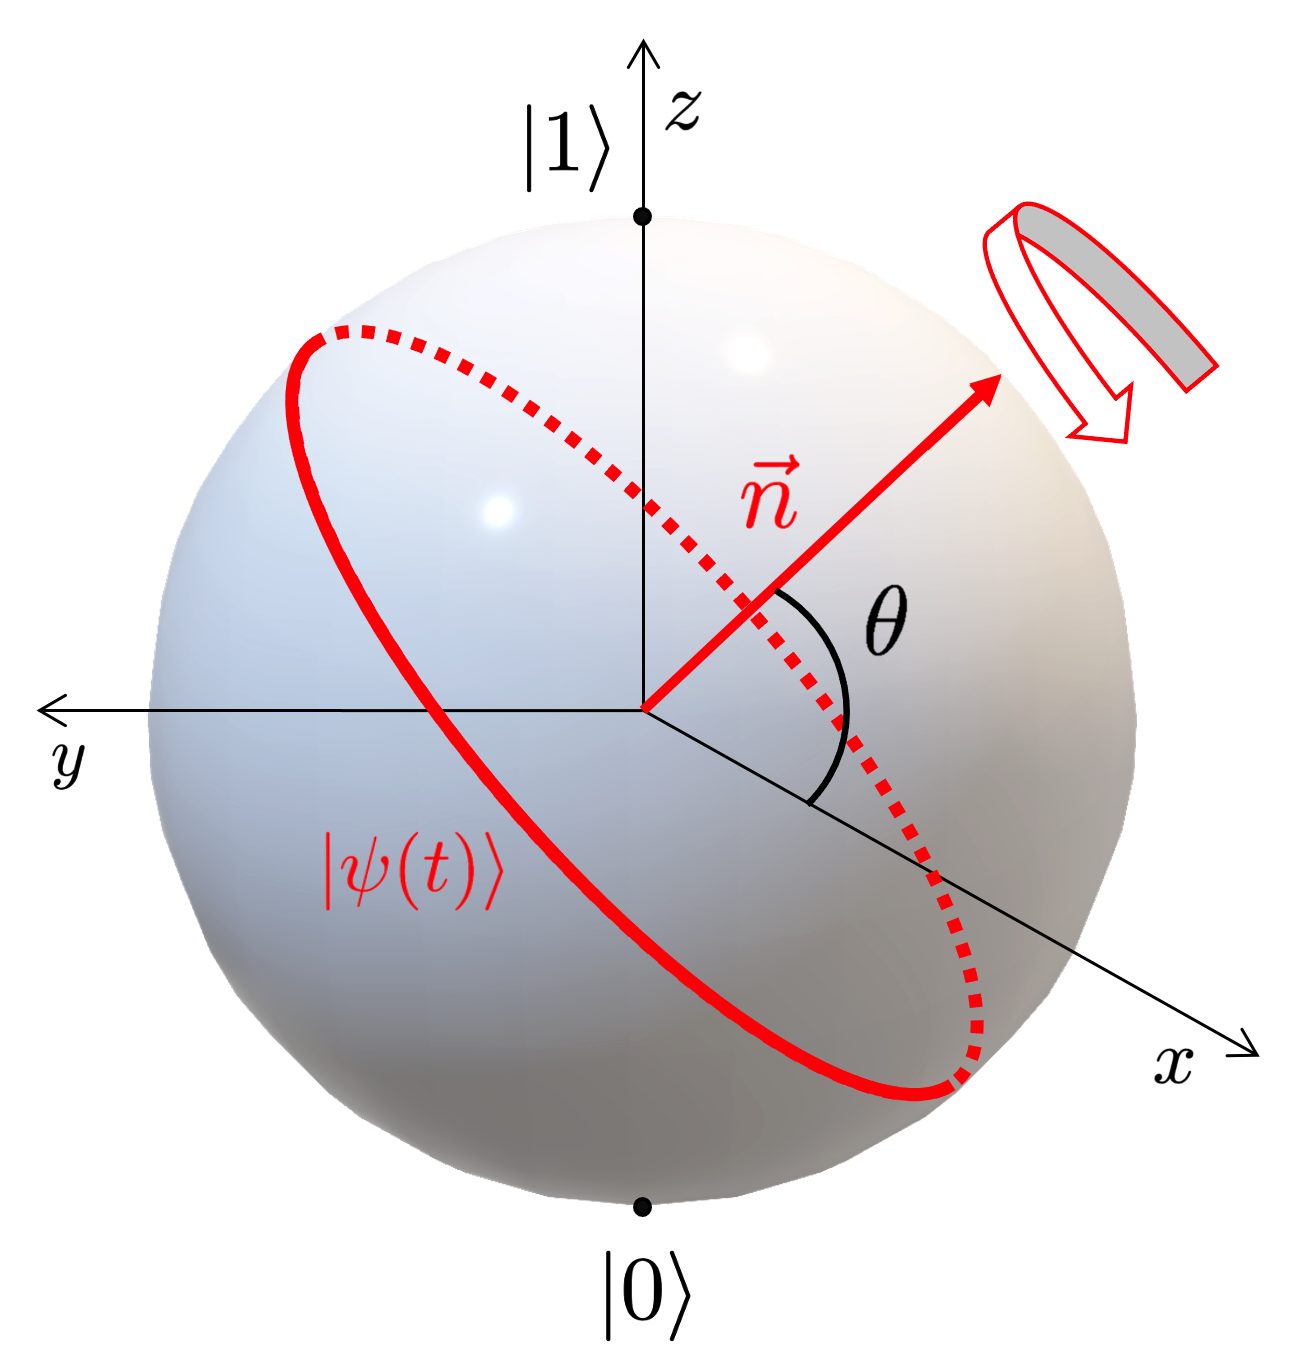
\includegraphics[width=0.42\linewidth]{images/Driven_two-level_system.png}
    \caption{Scheme of a driven two-level system with the Bloch sphere. The state $\ket{\psi(t)}$ is on the red circumference and it rotates with frequency $2 \Tilde{\Omega}$ around the vector $\Vec{n}$.}
    \label{fig:Bloch_sphere}
\end{figure}

\section{Time-independent degenerate perturbation theory}
\label{sec:timedep}

Consider a system described by the time-independent Hamiltonian $H = H_0 + \lambda V$, where $\lambda V$ is a perturbation (small when $\lambda \to 0$) and $H_0$ is the unperturbed Hamiltonian. The latter has eigenstates obtained by solving the eigenvalue equation: 
\begin{align*}
    H_0 \ket{\varepsilon^{(0)}_n, J} = \varepsilon^{(0)}_n \ket{\varepsilon^{(0)}_n, J}, 
\end{align*}
where $J$ is an index introduced to take into account the degeneracy of the states. 
The eigenvalue equation for the perturbed system is instead: 
\begin{align}
    \label{eq:SchEq_pert}
    (H_0 + \lambda V) \ket{\Tilde{\varepsilon}_n,J}= \Tilde{\varepsilon}_n \ket{\Tilde{\varepsilon}_n,J}, 
\end{align}
If $\lambda$ is small, $\ket{\Tilde{\varepsilon}_n}$ and $\Tilde{\varepsilon}_n$ can be written as a series expansion which takes into account the corrections to $\ket{\varepsilon^{(0)}_n}$ and $\varepsilon^{(0)}_n$:
\begin{align*}
    \Tilde{\varepsilon}_n &= \varepsilon^{(0)}_n + \lambda \varepsilon^{(1)}_n + \lambda^2 \varepsilon^{(2)}_n + ... \\
    \ket{\Tilde{\varepsilon}_n,J} &= \ket{\varepsilon^{(0)}_n,J_0} + \lambda \ket{\varepsilon^{(1)}_n,J_1} + \lambda^2 \ket{\varepsilon^{(2)}_n,J_2} + ...
\end{align*}
Inserting these expressions at first order in (\ref{eq:SchEq_pert})
\begin{align*}
    (H_0 + \lambda V) \left(\ket{\varepsilon^{(0)}_n,J_0} + \lambda \ket{\varepsilon^{(1)}_n,J_1} \right) = \left( \varepsilon^{(0)}_n + \lambda \varepsilon^{(1)}_n \right)\left(\ket{\varepsilon^{(0)}_n,J_0} + \lambda \ket{\varepsilon^{(1)}_n,J_1} \right)
\end{align*}
and considering only the terms at the same order in $\lambda$, it is possible to find the corrections to the unperturbed values. The zeroth order is trivial, while the first order gives:
\begin{align}
    \label{eq:fo_pert1}
    V \ket{\varepsilon^{(0)}_n,J_0} + H_0 \ket{\varepsilon^{(1)}_n,J_1} = \varepsilon^{(1)}_n \ket{\varepsilon^{(0)}_n,J_0} + \varepsilon^{(0)}_n \ket{\varepsilon^{(1)}_n,J_1}
\end{align}
Now it is useful to introduce the projector onto the $\varepsilon^{(0)}_n$ eigenspace of $H_0$
\begin{align*}
    \Pi_{\varepsilon^{(0)}_n} = \sum_{J} \ket{\varepsilon^{(0)}_n, J} \bra{\varepsilon^{(0)}_n, J}
\end{align*}
and to multiply it to the left in equation (\ref{eq:fo_pert1}): 
\begin{align*}
    \Pi_{\varepsilon^{(0)}_n} V \ket{\varepsilon^{(0)}_n,J_0} + \Pi_{\varepsilon^{(0)}_n} H_0 \ket{\varepsilon^{(1)}_n,J_1} &= \varepsilon^{(1)}_n \Pi_{\varepsilon^{(0)}_n} \ket{\varepsilon^{(0)}_n,J_0} + \varepsilon^{(0)}_n \Pi_{\varepsilon^{(0)}_n} \ket{\varepsilon^{(1)}_n,J_1} \\
     \Pi_{\varepsilon^{(0)}_n} V \ket{\varepsilon^{(0)}_n,J_0} +  H_0 \Pi_{\varepsilon^{(0)}_n} \ket{\varepsilon^{(1)}_n,J_1} &= \varepsilon^{(1)}_n  \ket{\varepsilon^{(0)}_n,J_0} + \varepsilon^{(0)}_n \Pi_{\varepsilon^{(0)}_n} \ket{\varepsilon^{(1)}_n,J_1} \\
      \Pi_{\varepsilon^{(0)}_n} V \ket{\varepsilon^{(0)}_n,J_0} +  \cancel{\varepsilon^{(0)}_n \Pi_{\varepsilon^{(0)}_n} \ket{\varepsilon^{(1)}_n,J_1}} &= \varepsilon^{(1)}_n  \ket{\varepsilon^{(0)}_n,J_0} + \cancel{\varepsilon^{(0)}_n \Pi_{\varepsilon^{(0)}_n} \ket{\varepsilon^{(1)}_n,J_1}},
\end{align*}
where the fact that $ \Pi_{\varepsilon^{(0)}_n} H_0 = H_0 \Pi_{\varepsilon^{(0)}_n} =\varepsilon^{(0)}_n \Pi_{\varepsilon^{(0)}_n}$ is used. The last result obtained can be written as
\begin{equation}
    \label{eq:fo_pert2}
    \left( \Pi_{\varepsilon^{(0)}_n} V \Pi_{\varepsilon^{(0)}_n} \right) \ket{\varepsilon^{(0)}_n,J_0} = \varepsilon^{(1)}_n  \ket{\varepsilon^{(0)}_n,J_0} \qquad \forall J_0,
\end{equation}
since $\ket{\varepsilon^{(0)}_n,J_0} = \Pi_{\varepsilon^{(0)}_n} \ket{\varepsilon^{(0)}_n,J_0}$. The operator in brackets is called $H^{(1)} \equiv \Pi_{\varepsilon^{(0)}_n} V \Pi_{\varepsilon^{(0)}_n}$ and it is Hermitian, while equation (\ref{eq:fo_pert2}) is an eigenvalue equation. It states that the degeneracy is removed (since now the eigenstate of the unperturbed Hamiltonian is associated to an eigenvalue different from $\varepsilon^{(0)}_n$) and how the resolved states looks like. Moreover, it is important to notice that the resolved states are not a small correction from an arbitrary unperturbed state. 

\subsubsection{Higher orders of degeneracy-removing Hamiltonians}

With an approach similar to the one presented previously, it is possible to obtain the higher order Hamiltonians. Explicitly, up to the forth order, they are:
\begin{align}
    H^{(0)} =&~ H_0 \label{eq:H0} \\
    H^{(1)} =&~ \Pi_{\varepsilon^{(0)}_n} V \Pi_{\varepsilon^{(0)}_n} \label{eq:H1}\\
    H^{(2)} =&~\Pi_{\varepsilon^{(0)}_n} V R_{\varepsilon^{(0)}_n} V \Pi_{\varepsilon^{(0)}_n}  \label{eq:H2} \\
    H^{(3)} =&~ \Pi_{\varepsilon^{(0)}_n} V R_{\varepsilon^{(0)}_n} V R_{\varepsilon^{(0)}_n} V \Pi_{\varepsilon^{(0)}_n} + \nonumber \\
    &- \Pi_{\varepsilon^{(0)}_n} V \Pi_{\varepsilon^{(0)}_n} V R_{\varepsilon^{(0)}_n}^2 V \Pi_{\varepsilon^{(0)}_n} \label{eq:H3} \\
    H^{(4)} =&~ \Pi_{\varepsilon^{(0)}_n} V R_{\varepsilon^{(0)}_n} V R_{\varepsilon^{(0)}_n} V R_{\varepsilon^{(0)}_n} V \Pi_{\varepsilon^{(0)}_n} + \nonumber \\
    & -\Pi_{\varepsilon^{(0)}_n} V R_{\varepsilon^{(0)}_n}^2 V \Pi_{\varepsilon^{(0)}_n} V R_{\varepsilon^{(0)}_n} V \Pi_{\varepsilon^{(0)}_n} + \nonumber \\
    &- \Pi_{\varepsilon^{(0)}_n} V \Pi_{\varepsilon^{(0)}_n} V R_{\varepsilon^{(0)}_n} V R_{\varepsilon^{(0)}_n}^2 V \Pi_{\varepsilon^{(0)}_n} + \nonumber \\
    &+ \Pi_{\varepsilon^{(0)}_n} V \Pi_{\varepsilon^{(0)}_n} V R_{\varepsilon^{(0)}_n}^2 V R_{\varepsilon^{(0)}_n} V \Pi_{\varepsilon^{(0)}_n} + \nonumber \\
    &+ \Pi_{\varepsilon^{(0)}_n} V \Pi_{\varepsilon^{(0)}_n} V \Pi_{\varepsilon^{(0)}_n} V R_{\varepsilon^{(0)}_n}^3 V \Pi_{\varepsilon^{(0)}_n} \label{eq:H4}
\end{align}
In these expressions, the \textit{Moore-Penrose pseudoinverse} $R_{\varepsilon^{(0)}_n}$ is introduced and it is defined as:
\begin{equation}
    R_{\varepsilon^{(0)}_n} = \left(\varepsilon^{(0)}_n \mathbb{I} - H_0 \right)^{``-1"}.
\end{equation}

The higher order degeneracy-removing Hamiltonians are applied to an important system in order to see explicitly their effect on the energy levels and on the states. 

\begin{tcolorbox}[breakable, enhanced]
\textbf{The three-level system ($\Lambda$ system) with perturbation theory} \\
Consider a system with three states
\begin{align*}
    \ket{0} = \begin{pmatrix} 1 \\ 0 \\ 0 \end{pmatrix}, \qquad \qquad \ket{e} = \begin{pmatrix} 0 \\ 1 \\ 0 \end{pmatrix} \qquad \text{and} \qquad \ket{1} = \begin{pmatrix} 0 \\ 0 \\ 1 \end{pmatrix},
\end{align*}
and with unperturbed Hamiltonian given by 
\begin{align*}
    H_0 = \begin{pmatrix} 0 & 0 & 0 \\ 0 & \Delta & 0 \\ 0 & 0 & 0 \end{pmatrix}.
\end{align*}
This implies that the states $\ket{0}$ and $\ket{1}$ are degenerate with energy $\varepsilon_1^{(0)} = \varepsilon_2^{(0)} = 0$, while the state $\ket{e}$ has energy $\epsilon_3^{(0)} = \Delta$. Consider now a small perturbation described by the term
\begin{align*}
    V = \begin{pmatrix} 0 & \Omega & 0 \\ \Omega & 0 & \Omega \\ 0 & \Omega & 0 \end{pmatrix} = \Omega \begin{pmatrix} 0 & 1 & 0 \\ 1 & 0 & 1 \\ 0 & 1 & 0 \end{pmatrix}. 
\end{align*}
The first two orders of degeneracy-removing Hamiltonians can be found considering the projectors and the Moore-Penrose pseudoinverse matrices
\begin{align*}
    \Pi_0 &= \begin{pmatrix} 1 & 0 & 0 \\ 0 & 0 & 0 \\ 0 & 0 & 1 \end{pmatrix} \qquad
    R_0 = \begin{pmatrix} 0 & 0 & 0 \\ 0 & -1/\Delta & 0 \\ 0 & 0 & 0 \end{pmatrix} \\ \Pi_\Delta &= \begin{pmatrix} 0 & 0 & 0 \\ 0 & 1 & 0 \\ 0 & 0 & 0 \end{pmatrix} 
    \qquad R_\Delta = \begin{pmatrix} 1/\Delta & 0 & 0 \\ 0 & 0 & 0 \\ 0 & 0 & 1/\Delta \end{pmatrix} 
\end{align*}
and inserting them in (\ref{eq:H1}) and (\ref{eq:H2}):
\begin{align*}
    H^{(1)}_0 &= \Pi_0 V \Pi_0 = 0 \\
    H^{(1)}_\Delta &= \Pi_\Delta V \Pi_\Delta = 0  \\
    H^{(2)}_0 &= \Pi_0 V R_0 V \Pi_0 = -\frac{\Omega^2}{\Delta} \begin{pmatrix} 1 & 0 & 1 \\ 0 & 1 & 0 \\ 1 & 0 & 1 \end{pmatrix} \\
    H^{(2)}_\Delta &= \Pi_\Delta V R_\Delta V \Pi_\Delta = \frac{2 \Omega^2}{\Delta} \begin{pmatrix} 0 & 0 & 0 \\ 0 & 1 & 0 \\ 0 & 0 & 0 \end{pmatrix} \label{eq:H_Delta}
\end{align*}
The matrix $H^{(2)}_0$ can be diagonalized in order to find the new eigenvalues after the perturbation; they are
\begin{align*}
    \varepsilon^{(2)}_a = -\frac{2 \Omega^2}{\Delta} \qquad \text{and} \qquad \varepsilon^{(2)}_b = 0.
\end{align*}
It is possible to notice that the last state is transparent to the perturbation ($\varepsilon_2^{(2)} = 0$) and it is called \textit{dark state}. The other state is shifted to a lower energy equal to $\varepsilon_1^{(2)} = -2 \Omega^2/\Delta$.

The matrix $H^{(2)}_\Delta$ is already diagonalized and from it is evident that the energy of the initial excited state $\ket{e}$ increases of $2 \Omega^2/\Delta$; therefore, $\varepsilon_3^{(2)} = \Delta\left( 1 + {2 \Omega^2}/{\Delta^2}\right)$. Obviously, these corrections are negligible if $\Omega \ll \Delta$ and hence if the perturbation is small.
\\

A scheme of the system without and with the perturbation is reported in figure \ref{fig:lambda_sys}. 
\end{tcolorbox}

The same results can be obtained with a conventional approach without the perturbation theory. 

\begin{tcolorbox}[breakable, enhanced]
\textbf{The $\Lambda$ system without perturbation theory} \\
Now the same system of the previous example is studied without applying perturbation theory. The total Hamiltonian can be written as 
\begin{align*}
    H = \Delta \begin{pmatrix} 0 & \eta & 0 \\ \eta & 1 & \eta \\ 0 & \eta & 0 \end{pmatrix} \qquad \text{with} \qquad \eta = \frac{\Omega}{\Delta}.
\end{align*}

The eigenvalues are obtained diagonalizing the matrix:
\begin{align*}
    p(\alpha) &= \alpha^2 (1-\alpha) + 2 \alpha \eta^2 = -\alpha (\alpha^2 - \alpha - 2 \eta^2) \\
    p(\alpha) &= 0 \quad \implies \quad \alpha = 0, ~~\alpha = \frac{1}{2} \left( 1 \pm \sqrt{1+ 8 \eta^2}\right).
\end{align*}
For small values of $\eta$, the eigenvalues are:
\begin{align*}
    \varepsilon_1 &\simeq \frac{\Delta}{2} -\frac{\Delta}{2}(1 + 4 \eta^2) = - \frac{2 \Omega^2}{\Delta} \\
    \varepsilon_2 &= 0 \\
    \varepsilon_3 &\simeq \frac{\Delta}{2} + \frac{\Delta}{2}(1 + 4 \eta^2) = \Delta\left( 1 + \frac{2 \Omega^2}{\Delta^2}\right).
\end{align*}
The results are consistent with the expressions for $\varepsilon_1^{(2)}$, $\varepsilon_2^{(2)}$ and $\varepsilon_3^{(2)}$ obtained in the previous example. 
\end{tcolorbox}

\begin{figure}[H]
\centering
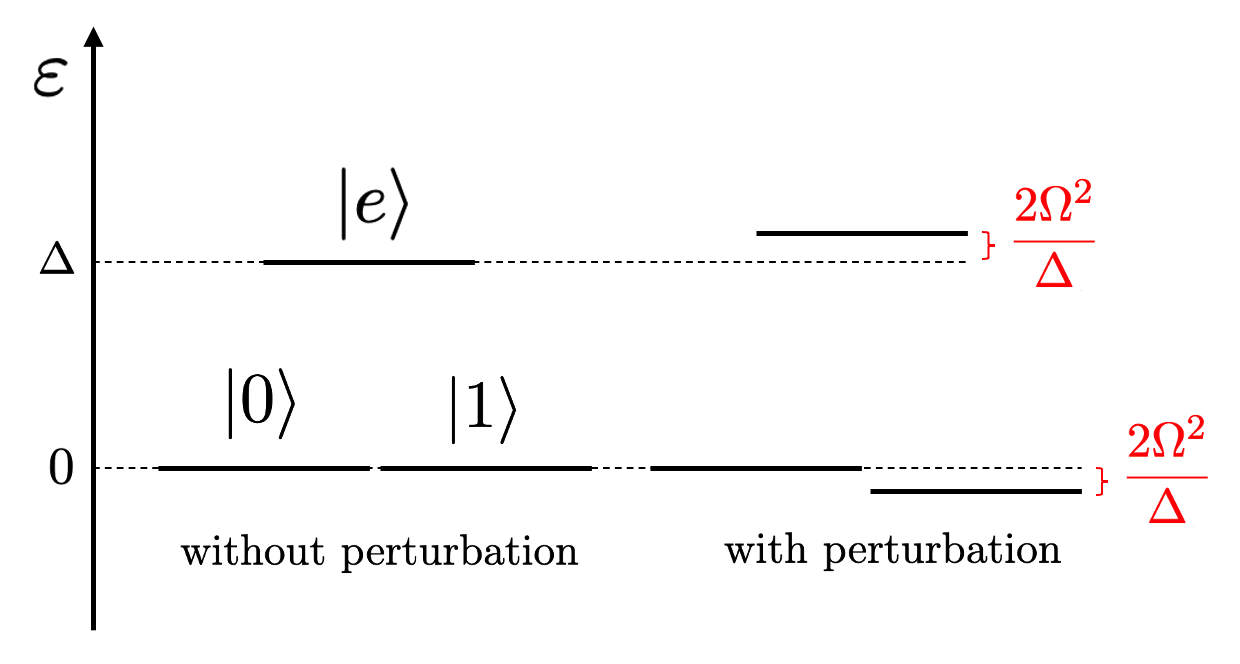
\includegraphics[width=0.66\linewidth]{images/Lambda_system.png}
    \caption{Scheme of a $\Lambda$ system without and with perturbation; it modifies the energy levels by removing the degeneracy and by increasing the separation between the ground states and the excited state.}
    \label{fig:lambda_sys}
\end{figure}

Some other considerations about the $\Lambda$ system can be done. First of all, the behaviour of the system for different values of the parameter $\Omega$ can be schematized as in figure \ref{fig:deg_rem}, where the degeneracy removal is evident. \\
Moreover, it is important to underline that it presents two typical energies (and hence two typical frequencies) $\Omega$ and $\Delta$ which can be associated to two characteristic motions of the system. The first one is related to the oscillations between the states $\ket{0}$ and $\ket{1}$ which happens with frequency $2 \Omega^2/\Delta$; it is named \textit{secular motion} because it is slow ($\Delta \gg \Omega$). The second one is related to the wiggles of the excited state $\ket{e}$ which are described by a frequency proportional to $\Delta$; it is named \textit{micromotion} because it is fast. 

\begin{figure}[t!]
\centering
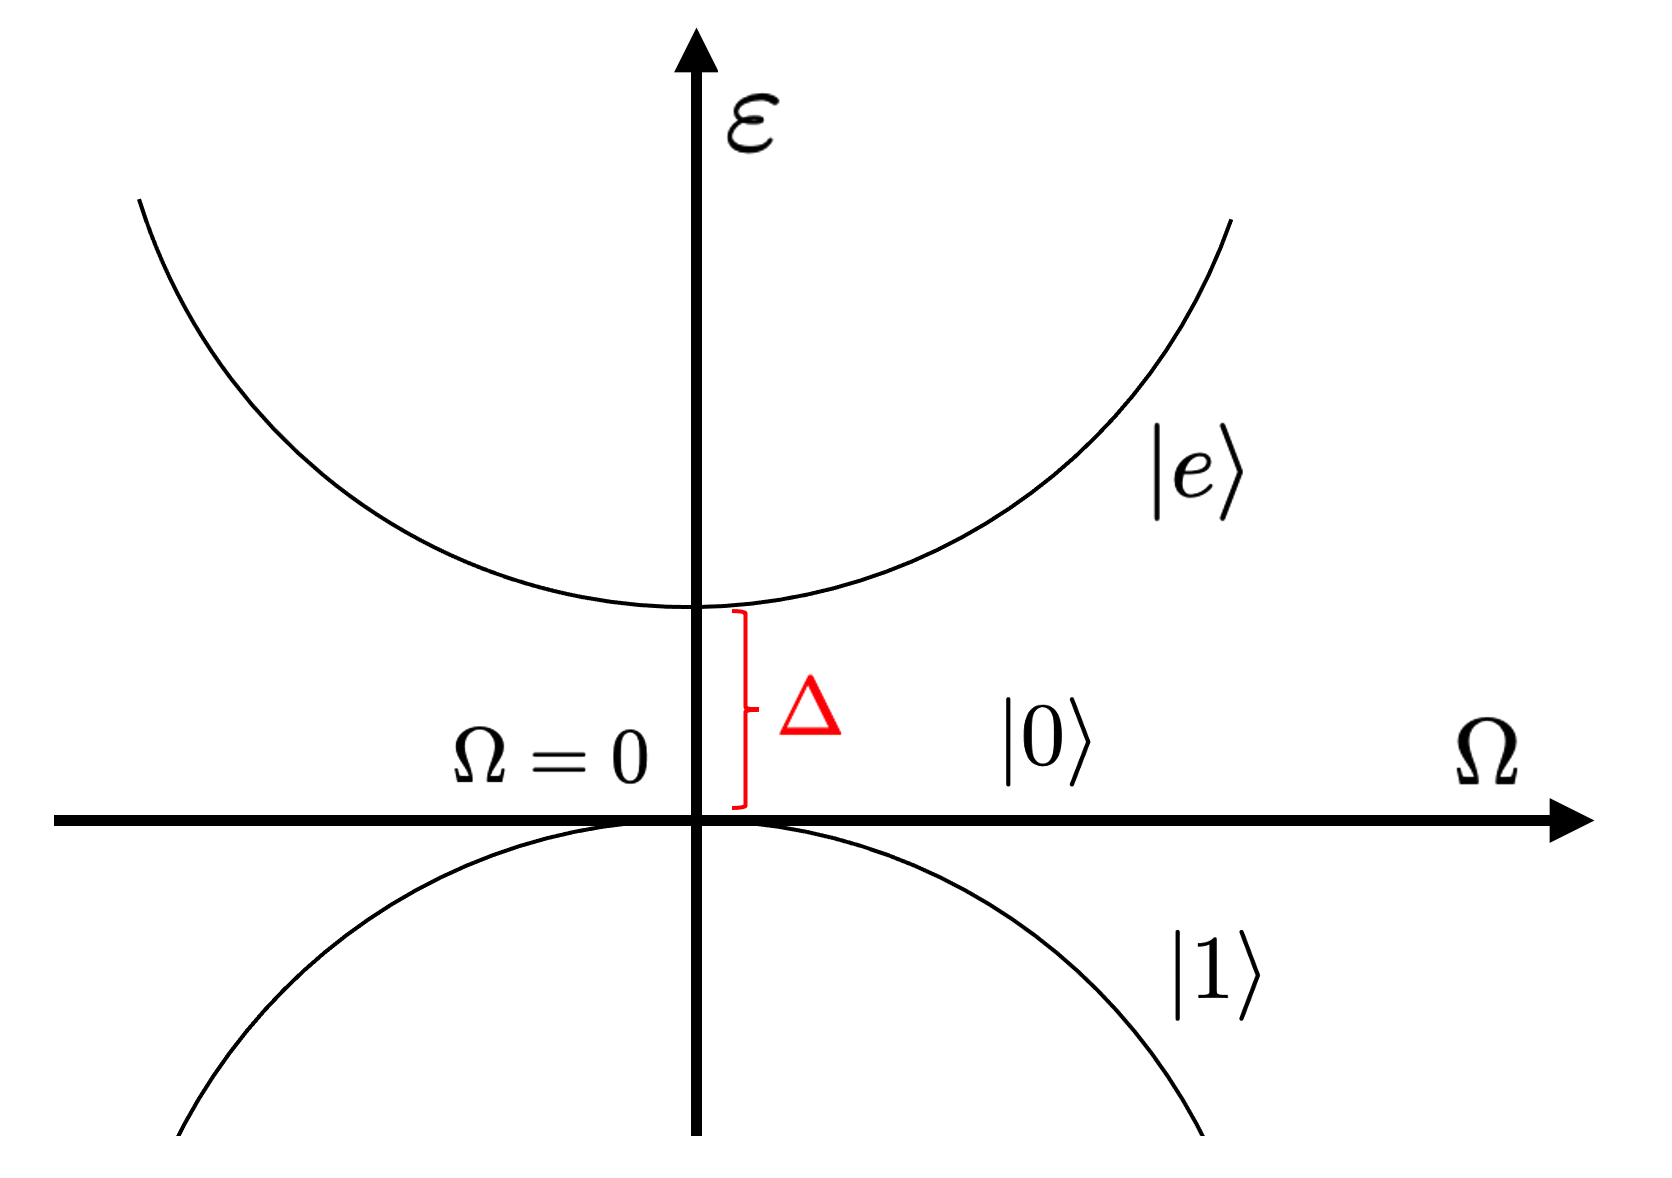
\includegraphics[width=0.61\linewidth]{images/Degeneracy_removal.png}
    \caption{Degeneracy removal in the $\Lambda$ system. For larger values of $\Omega$, the energy separation between the state $\ket{0}$ and the state $\ket{1}$ increases.}
    \label{fig:deg_rem}
\end{figure}

\section{Time-dependent Hamiltonians}
\label{sec:time_dep_sys}

\subsection{Time-ordered exponentials}

The Schr\"odinger equation with time-dependent Hamiltonian is 
\begin{equation}
    \label{eq:Schtime}
    i \hbar \frac{d}{dt}\ket{\psi(t)} = H(t)\ket{\psi(t)} \qquad \qquad \ket{\psi(t)} = U(t,t_0) \ket{\psi(t_0)}, 
\end{equation}
where $U$ is an unitary operator such that 
\begin{align*}
    U(t_2,t_1) U(t_1,t_0) = U(t_2,t_0) \qquad \text{additivity,} \\
    U(t,t) = \mathbb{I} \qquad \text{identity connection.}
\end{align*}
Equation (\ref{eq:Schtime}) can be rewritten in order to obtain an equation for $U(t,t_0)$:
\begin{equation}
    \label{eq:Utime}
    i \hbar \frac{dU}{dt} \cancel{\ket{\psi(t_0)}}= H(t) U(t,t_0) \cancel{\ket{\psi(t_0)}}.
\end{equation}
Consider now a small time increment $\delta t$ such that $U(t+\delta t,t_0)$ can be Taylor expanded
\begin{align*}
    U(t+\delta t,t_0) = U(t+\delta t,t) \, U(t,t_0) = U(t,t_0) + \delta t \frac{d U}{dt} + O(\delta t^2)
\end{align*}
and using equation (\ref{eq:Utime}) becomes 
\begin{align*}
    U(t+\delta t,t) \, \cancel{U(t,t_0)} = \cancel{U(t,t_0)} - \frac{i}{\hbar} \delta t \, H(t) \cancel{U(t,t_0)} + O(\delta t^2) \\
    U(t+\delta t,t) =\mathbb{I} - \frac{i}{\hbar} \delta t \, H(t) + O(\delta t^2) \simeq \exp{- \frac{i}{\hbar} \delta t \, H(t)}.
\end{align*}
The same calculations can be done for several infinitesimal time increments which allow to write $U(t,t_0)$ as 
\begin{align*}
    U(t,t_0) &= U(t,t-\delta t) \, U(t,t-2\delta t) \, ... \, U(t_0 + \delta t_0, t_0) \simeq \\
    &\simeq \exp{-\frac{i}{\hbar} \delta t \, H(t-\delta t)}  \exp{-\frac{i}{\hbar} \delta t \, H(t-2\delta t)} \, ... \, \exp{- \frac{i}{\hbar} \delta t \, H(t_0)} \overset{\delta t \to 0}{\equiv} \\
    &\overset{\delta t \to 0}{\equiv}  \mathcal{T}\exp{-\frac{i}{\hbar} \int_{t_0}^{t} H(t')dt'}. 
\end{align*}
The last lines are the definition of the \textit{time-ordered exponential} if $\delta t \to 0$; it is related to the well-known Dyson series which provide an analogous expression for $U(t,t_0)$. 
\begin{align*}
    U(t,t_0) = \mathbb{I} + \sum_{n=1}^\infty (-i)^n \int_{t_0}^{t} dt_1 \int_{t_0}^{t_1} dt_2 \, ... \, \int_{t_0}^{t_{n-1}} dt_n H(t_1) H(t_2) \, ... \, H(t_n)
\end{align*}

\subsection{Time-periodic system}
\label{subsec:1.5.2}
Consider the Hamiltonian 
\begin{equation}
    H(t) = H_0 + W(t),
\end{equation}
where $H_0$ describes the system and $W(t)$ is the external potential, also called \textit{drive}. By changing $H_0$ and $W(t)$ it is possible to control the system and to design some properties of it, but in general the solutions are not trivial. A simplified situation is the one in which the external potential is periodic: $W(t+T) = W(t)$; in this case, it is useful to study the \textit{time-averaged behaviour} of the system. 

The first step consists in writing the statevector $\ket{\psi(t)}$ in a new basis in order to introduce the state $\ket{\psi'(t)} = R(t) \ket{\psi(t)}$, where $R(t)$ is an unitary operator which therefore can be written as 
\begin{align*}
    R(t) = e^{i K(t)},
\end{align*}
where $K(t)$ is Hermitian. The Schr\"odinger equation for the system becomes 
\begin{align*}
    i \hbar \frac{d}{dt} \ket{\psi(t)} &= H(t)  \ket{\psi(t)} \\
    i \hbar \frac{d}{dt} \left( R^\dagger(t) \ket{\psi'(t)} \right) &= H(t) R^\dagger(t) \ket{\psi'(t)} \\
    i \hbar \, \frac{dR^\dagger(t)}{dt} \ket{\psi'(t)} + i \hbar \, R^\dagger(t) \frac{d}{dt} \ket{\psi'(t)} &= H(t) R^\dagger(t) \ket{\psi'(t)}.
\end{align*}
Multiplying by $R(t)$ on the left
\begin{align*}
    i \hbar \, R(t) \frac{dR^\dagger(t)}{dt} \ket{\psi'(t)} + i \hbar \,R(t) R^\dagger(t) \frac{d}{dt} \ket{\psi'(t)} &= R(t) H(t) R^\dagger(t) \ket{\psi'(t)}
\end{align*}
from which 
\begin{align*}
    i \hbar \frac{d}{dt} \ket{\psi'(t)} &= R(t) H(t) R^\dagger(t) \ket{\psi'(t)} - i \hbar R(t) \frac{dR^\dagger(t)}{dt} \ket{\psi'(t)} \\
    &= \left( R(t) H(t) R^\dagger(t) - i \hbar R(t) \frac{dR^\dagger(t)}{dt} \right) \ket{\psi'(t)}
\end{align*}
This is a Schr\"odinger equation for $\ket{\psi'(t)}$ with Hamiltonian 
\begin{align}
    H'(t) = R(t) H(t) R^\dagger(t) - i \hbar R(t) \frac{dR^\dagger(t)}{dt}. 
    \label{eq:transfH}
\end{align}
It is straightforward to show\footnote{The time-dependece is omitted in this proof.} that $H'(t)$ is Hermitian starting from
\begin{align*}
    H' &= R H R^\dagger - i \hbar R \frac{dR^\dagger}{dt} \\
    H'^\dagger &= R H^\dagger R^\dagger + i \hbar \left( \frac{d R^\dagger}{dt} \right)^\dagger R^\dagger = R H R^\dagger + i \hbar \frac{dR}{dt} R^\dagger
\end{align*}
and considering
\begin{align*}
    H'- H'^\dagger &= -i R \frac{d R^\dagger}{dt} - i \frac{d R}{dt} R^\dagger = \\
    &= -i\left( R \frac{d R^\dagger}{dt} + \frac{d R}{dt} R^\dagger \right) \\
    &= -i \frac{d}{dt} (R R^\dagger) = -i \frac{d \mathbb{I}}{dt} = 0. 
\end{align*}
Therefore,
\begin{align}
    \label{eq:Hprim}
    H'(t) = R(t) H(t) R^\dagger(t) - i \hbar R(t) \frac{dR^\dagger(t)}{dt} = R(t) H(t) R^\dagger(t) + i \hbar \frac{dR(t)}{dt} R^\dagger(t) 
\end{align}


It is interesting to notice that $H'(t)$ in (\ref{eq:Hprim}) can be built in such a way that it is time-independent ($H'(t) = H'$). The simplest way to achieve this condition is to start from a time-dependent Hamiltonian of the form
\begin{equation}
    \label{eq:start_ham}
    H(t) = H_0 + e^{i \omega t} V + e^{-i \omega t} V^\dagger,
\end{equation}
in which the periodic potential is monochromatic (fixed oscillation frequency) with $\omega \gg \Delta E/\hbar$ (\textit{high-frequency approximation}), where $\Delta E$ is the typical energy scale of $H_0$. In this case, assume that one can write the operators $H'$ and $K(t)$ in the general form
\begin{align*}
    H' = \sum_n \frac{1}{\omega^n} H'_n \qquad \text{and} \qquad
    K(t) = \sum_n \frac{1}{\omega^n} K_n(t);
\end{align*}
inserting these considerations in (\ref{eq:Hprim}), one can obtain
\begin{equation}
    \label{eq:final_ham}
    H' = H_0 + \frac{1}{\hbar \omega} [V,V^\dagger] + \frac{1}{2 (\hbar \omega)^2} \left( [[V,H_0],V^\dagger] + [[V^\dagger,H_0],V] \right) + O\left( \frac{1}{\omega^3} \right)
\end{equation}
in the case in which 
\begin{equation}
    \label{eq:K}
    K(t) = \frac{1}{i \hbar \omega } V e^{i \omega t} - \frac{1}{i \hbar \omega} V^\dagger e^{-i \omega t} + O \left( \frac{1}{\omega^2} \right). 
\end{equation}
It is important to underline that relations (\ref{eq:final_ham}) and (\ref{eq:K}) are approximated expressions which are valid only in the high-frequency regime, the most general relation for $H'(t)$ is (\ref{eq:Hprim}). Moreover, in this regime, it is possible to identify a fast dynamics (micro-motion) associated to the operator $K(t)$ and a slow dynamics (secular motion) associated to the operator $H'(t)$.

\begin{tcolorbox}[breakable, enhanced]
\textbf{Qubit system with a \textit{weak drive} in the high-frequency regime} \\
Consider the Hamiltonian of a two-level system
\begin{align}
    \label{eq:qubit_H0}
    H_0 = -J \sigma^x = -J \begin{pmatrix} 0 & 1 \\ 1 & 0 \end{pmatrix} 
\end{align}
and the periodic potential
\begin{align}
    \label{eq:qubit_W}
    W(t) = \Delta \cos{(\omega t)} \, \sigma^z = \frac{\Delta}{2} e^{i \omega t} \sigma^z + \frac{\Delta}{2} e^{-i \omega t} \sigma^z,
\end{align}
with $\hbar \omega \gg \Delta$ (weak drive) and $\hbar \omega \gg J$ (high-frequency regime). Notice that $H(t) = H_0 + W(t)$ is in the form (\ref{eq:start_ham}) and that there are three characteristic energies: $J$ (strength of the Hamiltonian), $\Delta$ (strength of the drive) and $\hbar \omega$ (energy of the drive oscillations); moreover, $V = V^\dagger = (\Delta/2) \sigma^z$ and $\omega \gg J/\hbar$ (high frequency regime). 
From (\ref{eq:final_ham}), the Hamiltonian in the new reference frame is made of two parts (at the second order approximation)
\begin{align*}
    H'= H_0 + \frac{1}{2 (\hbar \omega)^2} \, 2 \, [[V,H_0],V] = H_0 + \frac{1}{(\hbar \omega)^2}  [[V,H_0],V]  ,
\end{align*}
which can be explicitly computed:
\begin{align*}
    &[V,H_0] = \left[ \frac{\Delta}{2} \sigma^z, J \sigma^x \right] = -\frac{J\Delta}{2} [\sigma^z,\sigma^x] = - i J \Delta \sigma^y, \\
    &[[V,H_0],V] = \left[-i J \Delta \sigma^y, \frac{\Delta}{2} \sigma^z \right] = -i \frac{J \Delta^2}{2} [\sigma^y, \sigma^z] = -J \Delta^2 \sigma^x.
\end{align*}
Therefore
\begin{align*}
    H' = -J \sigma^x + \frac{J \Delta^2}{(\hbar \omega)^2} \sigma^x = -J\left( 1 - \frac{\Delta^2}{(\hbar \omega)^2} \right) \sigma^x \equiv - J'\sigma^x
\end{align*}
and the operator $K(t)$ is given by
\begin{align*}
    K(t) = \frac{\Delta}{2 i \hbar \omega } e^{i \omega t} \sigma^z - \frac{\Delta}{2 i \hbar \omega } e^{-i \omega t} \sigma^z = \frac{\Delta}{\hbar\omega } \sin{(\omega t)} \, \sigma^z.
\end{align*}
The introduction of the time periodic perturbation causes a reduction of the energy scale of the unperturbed Hamiltonian $H_0$, indeed $J'< J$. Hence, the energy separation between the two states decreases, as shown in figure \ref{fig:quibit_drive}. This effect is called \textit{AC Stark shift}.\\ 
In the case of a weak drive (i.e. $\hbar \omega \gg \Delta$), the modification of the original energy levels is negligible. 
\end{tcolorbox}

\begin{figure}[H]
\centering
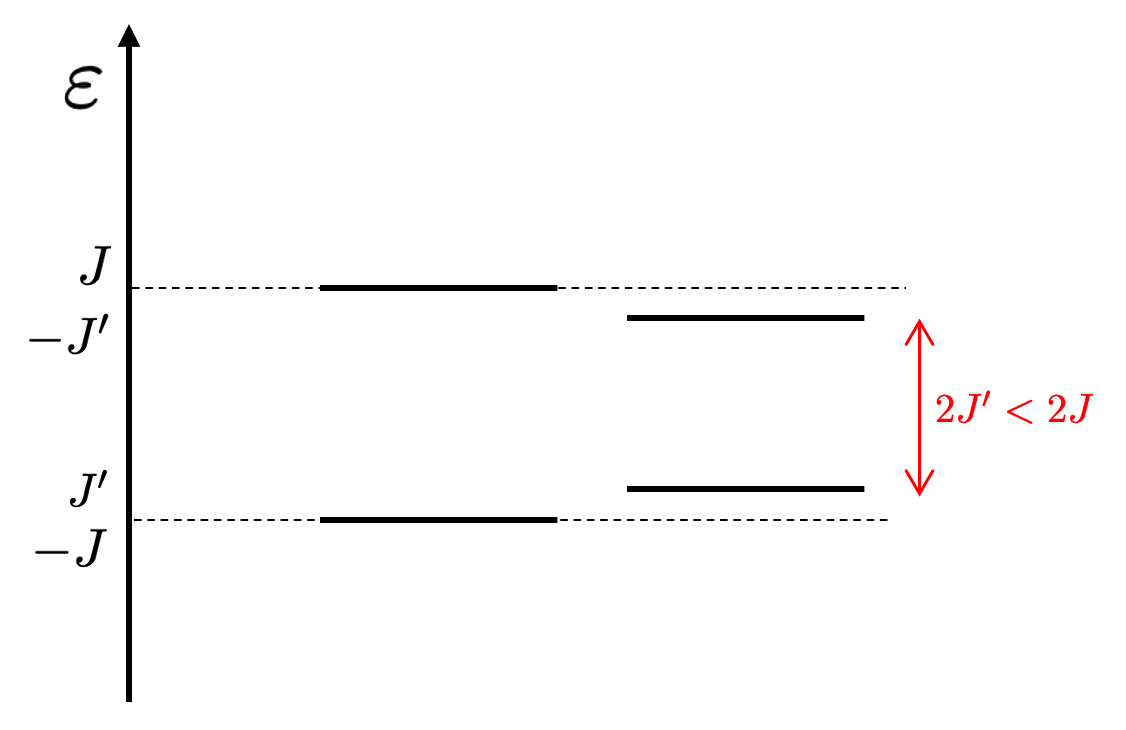
\includegraphics[width=0.58\linewidth]{images/Qubit_with_drive_1.png}
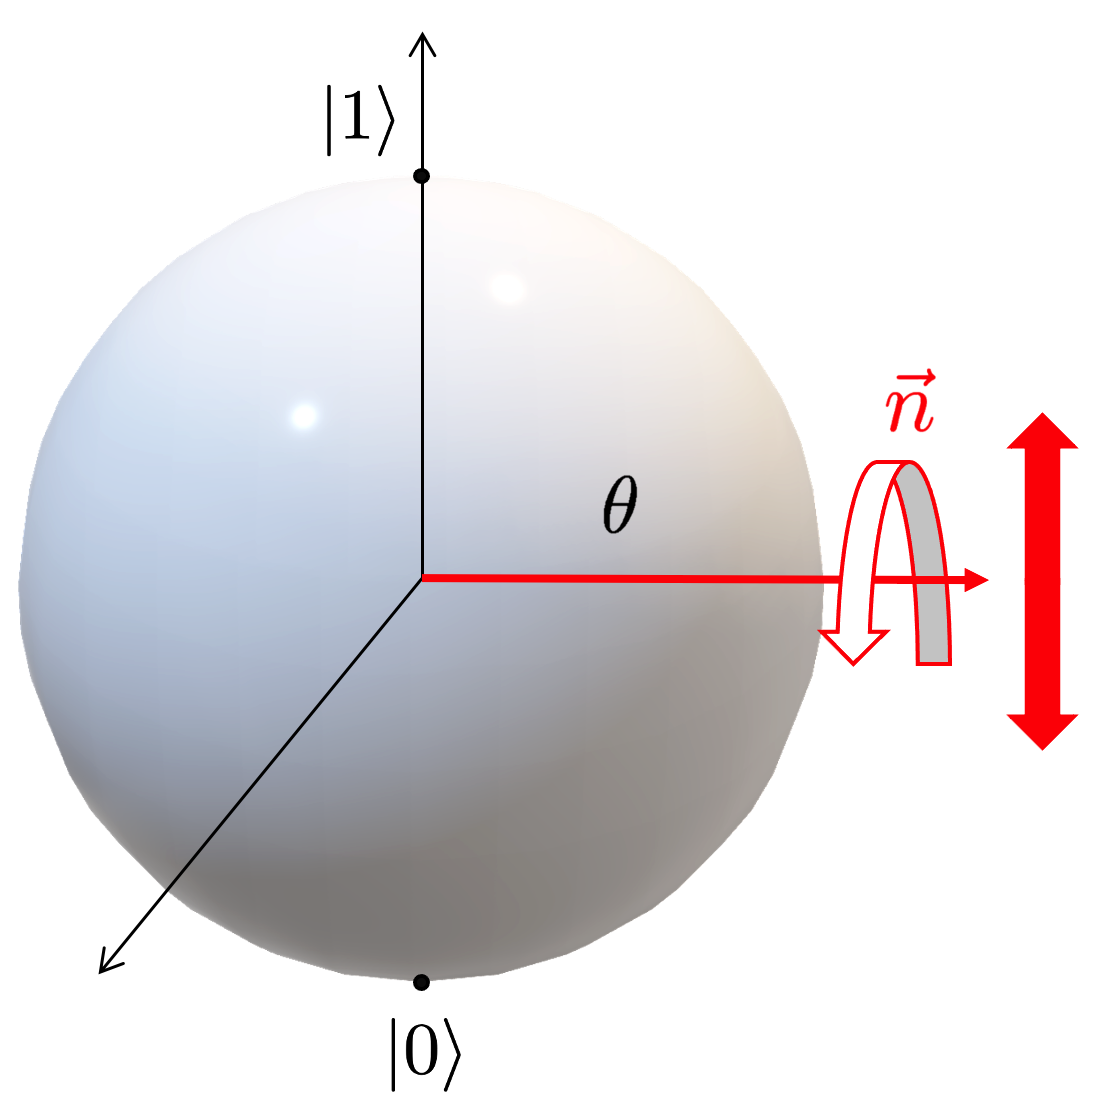
\includegraphics[width=0.37\linewidth]{images/Qubit_with_drive_2.png}
    \caption{Qubit with time periodic external potential. The system can be visualized also with a Bloch sphere which rotates around the red axis $\Vec{n}$ and which moves up and down.}
    \label{fig:quibit_drive}
\end{figure}

\begin{tcolorbox}[breakable, enhanced]
\textbf{Qubit system with a \textit{strong drive} in the high-frequency regime} \\
The aim is to study again the two-level system with the Hamiltonian (\ref{eq:qubit_H0}) and with the drive (\ref{eq:qubit_W}) but in the case in which $\hbar \omega \approx \Delta$ (strong drive).

To find the solution, one needs to reformulate the problem performing two steps: 
\begin{enumerate}
    \item $W(t)$ is removed by means of an exact unitary transformation (without expression (\ref{eq:final_ham}) and (\ref{eq:K}));
    \item another high-frequency expansion is done in the new frame (this can be done remembering that $\omega \gg J/\hbar$ is valid). 
\end{enumerate}
Summarizing, the procedure is
\begin{align*}
    \ket{\psi} \quad \xrightarrow[\text{exactly}]{R(t)} \quad \ket{\psi'} \quad \xrightarrow [\text{perturbatively}]{R'(t)} \quad \ket{\psi''}.
\end{align*}
For the first part, the transformation
\begin{align*}
    R(t) = e^{i K(t)} = \exp{i \frac{\Delta}{\hbar \omega} \sin{(\omega t)} \sigma^z}
\end{align*}
is used to obtain $H'(t)$ from (\ref{eq:Hprim}):
\begin{align*}
    R(t) H(t) R^\dagger(t) &= R(t) (H_0 + W(t)) ) R^\dagger(t) = \\
    &= R(t) H_0 R^\dagger(t) + R(t) W(t) R^\dagger(t) = \\
    &= R(t) H_0 R^\dagger(t) + W(t), \\
    \frac{dR^\dagger(t)}{dt} &= i \frac{\Delta}{\omega} \cos{(\omega t)} \omega \sigma^z \exp{-i\frac{\Delta}{\hbar \omega} \sin{(\omega t)} \sigma^z}, \\
    R(t) \frac{dR^\dagger(t)}{dt} &= -i\frac{\Delta}{\hbar} \cos{(\omega t)} R(t) \sigma^z R^\dagger(t) = \\
    &= \frac{\Delta}{\hbar} \cos{(\omega t)} \sigma^z,
\end{align*}
where it is exploited the fact that $[R(t),W(t)] = 0$ since both $R(t)$ and $W(t)$ are functions of $\sigma^z$. Therefore, 
\begin{align*}
    H'(t) &= R(t) H_0 R^\dagger(t) + W(t) - \Delta \cos{(\omega t)} \sigma^z = \\
    &= R(t) H_0 R^\dagger(t) = \\
    &= \exp{i \frac{\Delta}{\hbar \omega} \sin{(\omega t)} \sigma^z} H_0 \exp{-i \frac{\Delta}{\hbar \omega} \sin{(\omega t)} \sigma^z}
\end{align*}
The periodic potential is not present in $H'(t)$. \\
For the second part, $H'(t)$ must be rewritten in the form $H'(t) = H_0' + W'(t)$; in order to obtain this, consider the transformation $R(t)$ written as:
\begin{align*}
    R(t) = e^{i \theta (\Vec{n} \cdot \Vec{\sigma})} = \mathbb{I} \cos{\theta} + i (\Vec{n} \cdot \Vec{\sigma}) \sin{\theta} 
\end{align*}
with 
\begin{align*}
    \theta = \frac{\Delta}{\hbar \omega} \sin{(\omega t)}, \qquad \Vec{n} = \begin{pmatrix} 0 \\ 0 \\ 1 \end{pmatrix}, \qquad \text{and} \qquad \Vec{\sigma} = \begin{pmatrix} \sigma^x \\ \sigma^y \\ \sigma^z \end{pmatrix}.
\end{align*}
Remembering that $H_0 = -J \sigma^x = -J \, (\ket{0}\bra{1} + \ket{1}\bra{0})$, $H'(t)$ becomes 
\begin{align*}
    H'(t) &= R(t) H_0 R^\dagger(t) = \\
    &=- J \,  R(t)\, (\ket{0}\bra{1}) \, R^\dagger(t) - J \,  R(t)\, (\ket{1}\bra{0}) \, R^\dagger(t) = \\
    &= -J \, e^{2 i \theta}\, (\ket{0}\bra{1}) + \text{h.c.} \\
    &= -J \, \exp{2 i \frac{\Delta}{\hbar \omega} \sin{(\omega t)}}\, (\ket{0}\bra{1}) + \text{h.c.} \\
    &\equiv -J'(t)\, (\ket{0}\bra{1}) \, + \text{h.c.} 
\end{align*}
A Fourier decomposition of $J'(t)$ is allowed because one can always write 
\begin{align*}
    e^{i \alpha \sin(z)} = \sum_{n = -\infty}^{+\infty} \mathcal{J}_n(\alpha) \, e^{i n z},
\end{align*}
where $\mathcal{J}_n(\alpha)$ is a \textit{Bessel function} of the first kind at order $n$. In this case, $\alpha = 2 \Delta / (\hbar \omega)$ and $z = \omega t$; hence
\begin{align*}
    H'(t) &= -J \sum_{n = -\infty}^{+\infty} \mathcal{J}_n\left( \frac{2 \Delta}{\hbar \omega} \right) (\ket{0}\bra{1})\, e^{i n \omega t} + \text{h.c.} = \\
    &= -J \mathcal{J}_0 \left( \frac{2 \Delta}{\hbar \omega} \right) (\ket{0}\bra{1}) -J \sum\limits_{\substack{n=-\infty \\ n\neq 0}}^{+\infty} \mathcal{J}_n\left( \frac{2 \Delta}{\hbar \omega} \right) (\ket{0}\bra{1}) \, e^{i n \omega t} + \text{h.c.} = \\
     &= -J \mathcal{J}_0 \left( \frac{2 \Delta}{\hbar \omega} \right) \sigma^x -J \sum\limits_{\substack{n=-\infty \\ n\neq 0}}^{+\infty} \mathcal{J}_n\left( \frac{2 \Delta}{\hbar \omega} \right) (\ket{0}\bra{1}) \, e^{i n \omega t} + \text{h.c. ($n \neq 0$)} = \\
     &\equiv H_0' + W'(t). 
\end{align*}
Therefore, in this new frame, $H'(t)$ can be written in the form $H_0' + W'(t)$, where $H_0'$ is time-independent and $W'(t)$ represents a multi-frequency periodic part with general term which can be written as $V_n \, e^{i n \omega t}$. The expression is equivalent to (\ref{eq:start_ham}) and another perturbative approach in $\omega \gg J/\hbar$ allows to obtain an expression for the new Hamiltonian similar to (\ref{eq:final_ham}): 
\begin{align}
    H''(t) = H_0' + \frac{1}{\hbar \omega} \sum_{n,m= -\infty}^{+\infty} [V_n',V_m']  + O\left( \frac{1}{\omega^2}\right) \simeq - J \mathcal{J}_0\left( \frac{2 \Delta}{\hbar \omega} \right) \sigma^x, 
\end{align}
where the approximation at the end is done since $\omega \gg J/\hbar$ and $V_n'$ is proportional to $J$. Notice that $\Delta/(\hbar \omega)$ is a quantity without constrains and hence it could also be also $\hbar \omega \approx \Delta $. 

A final note is about the fact that for $\hbar \omega \gg \Delta$ one can write
\begin{align*}
    \mathcal{J}_0 \left( \frac{2 \Delta}{\hbar \omega} \right) \simeq 1 - \frac{1}{4}\left( \frac{2 \Delta}{\hbar \omega} \right)^4 = 1 - \frac{\Delta^2}{(\hbar \omega)^2}, 
\end{align*}
from which 
\begin{align*}
    H''(t) = -J \left(  1 - \frac{\Delta^2}{(\hbar \omega)^2} \right) \sigma^x.
\end{align*}
This result is the same obtained in the case of a weak regime. 
\end{tcolorbox}








\chapter{Open quantum systems}

An open quantum system is a quantum-mechanical system that interacts with an external quantum system, which is known as the environment or a \textit{bath}. First of all, to describe an open system and its evolution, it is necessary to introduce the concept of \textit{mixed state}. 

\section{Mixed states}

A mixed state can be seen as an ensemble of quantum states in which each of them has an associated probability:
\begin{align*}
    \ket{\psi} ~~\text{pure state} \quad \longrightarrow \quad \left( \ket{\psi_\alpha}, p_\alpha \right) ~~\text{mixed state with} ~~\sum_\alpha p_\alpha = 1. 
\end{align*}
The states $\ket{\psi_\alpha}$ do not interfere, while the $p_\alpha$ are classical probabilities.

\subsubsection{Ensemble average and density operator}
The ensemble average of an operator $O$ on a mixed state is given by 
\begin{align*}
    \langle O \rangle_\text{ensemble} &\equiv \sum_\alpha p_\alpha \bra{\psi_\alpha} O \ket{\psi_\alpha} = \sum_\alpha p_\alpha \text{Tr}[ \, O \, \ket{\psi_\alpha} \bra{\psi_\alpha} \,] = \\
    &= \text{Tr} \left[ O \left( \sum_\alpha p_\alpha \ket{\psi_\alpha} \bra{\psi_\alpha} \right) \right] \equiv \text{Tr}[O \rho],
\end{align*}
where in the last line the \textit{density operator} (matrix) is introduced:
\begin{equation}
    \rho = \sum_\alpha p_\alpha \ket{\psi_\alpha} \bra{\psi_\alpha}. 
\end{equation}
The operator $\rho$ contains all the information about the system which is investigated. \\
The main properties of the density matrix are:
\begin{enumerate}
    \item Each element is positive (``$\rho \geq 0$"), which means that $\forall \ket{\phi}, ~\bra{\phi} \rho \ket{\phi} \geq 0$
    \begin{align*}
        & \implies \rho ~\text{is Hermitian} ~~ \rho = \rho^\dagger, \\
        & \implies \rho ~\text{can be diagonalized}, \\
        & \implies \text{Spec}(\rho) \geq 0. 
    \end{align*}
    \item Its trace is normalized to 1: i.e. Tr$[\rho] = 1$. 
    \item It represents the mixing of states and this does not produce interference; indeed, consider two matrix operators $\rho_1$ and $\rho_2$ and define 
    \begin{align*}
        \rho_+ = \frac{1}{2} \rho_1 + \frac{1}{2} \rho_2;
    \end{align*}
    for a given state $\ket{\phi}$, one can introduce 
    \begin{align*}
        P_1 &\equiv \text{Tr}[\ket{\phi}\bra{\phi} \rho_1] = \bra{\phi} \rho_1 \ket{\phi} \\
        P_2 &\equiv \text{Tr}[\ket{\phi}\bra{\phi} \rho_2] = \bra{\phi} \rho_2 \ket{\phi} \\
        P_+ &\equiv \text{Tr}[\ket{\phi}\bra{\phi} \rho_+] = \bra{\phi} \rho_+ \ket{\phi} = \\
        &= \frac{1}{2} \bra{\phi} \rho_1 \ket{\phi} + \frac{1}{2} \bra{\phi} \rho_2 \ket{\phi} = \frac{P_1 + P_2}{2}. 
    \end{align*}
    The probability of having $\ket{\phi}$ from the sum of the two mixtures is given by the sum of the probabilities in $\rho_1$ and $\rho_2$. 
\end{enumerate}

\subsection{Quantifier of the determinism}
Two quantities can be introduced to described how much a state is pure or mixed:
\begin{itemize}
    \item \textit{Purity}: 
    \begin{equation}
        \label{eq:purity}
        \mathcal{P} = \text{Tr}[\rho^2] \qquad \text{with} \qquad \frac{1}{\text{dim}_S} \leq \text{Tr}[\rho^2] \leq 1
    \end{equation}
    and $\mathcal{P} = 1$ indicates a pure state. 
    \item \textit{Entropy}
    \begin{equation}
        \label{eq:entropy}
        \mathcal{S} = -\text{Tr}[\rho \log \rho] \qquad \text{with} \qquad 0 \leq \mathcal{S} \leq \log{(\text{dim}_S)}
    \end{equation}
    and $\mathcal{S} = 0$ indicates a pure state. The entropy increases when the one loses information about the system. Moreover, it is important to remember that the logarithm of an operator is define according to the Taylor expansion. 
\end{itemize}

\begin{tcolorbox} [breakable, enhanced]
\textbf{Discrete mixing of states} \\
Consider a mixture of two states $\ket{\psi_1}$ and $\ket{\psi_2}$ on the surface of the Bloch sphere, as represented in figure \ref{fig:mix_states1}, and in the $xz$ plane:
\begin{align*}
    \ket{\psi_1} = \begin{pmatrix} \cos{\theta} \\ \sin{\theta} \end{pmatrix} \qquad \text{and} \qquad \ket{\psi_2} = \begin{pmatrix} \cos{\theta} \\ -\sin{\theta} \end{pmatrix}
\end{align*}
It is straightforward to see that 
\begin{align*}
    \langle \sigma^x \rangle_{\psi_1} &= \sin{(2 \theta)} \qquad \langle \sigma^x \rangle_{\psi_2} = -\sin{(2 \theta)} \\  
    \langle \sigma^z \rangle_{\psi_1} &= \cos{(2 \theta)} \qquad \langle \sigma^z \rangle_{\psi_2} = \cos{(2 \theta)}
\end{align*}
and that $\langle \sigma^y \rangle_{\psi_1} = \langle \sigma^y \rangle_{\psi_2} = 0$. The density operator is 
\begin{align*}
    \rho = \frac{1}{2} \ket{\psi_1}\bra{\psi_1} + \frac{1}{2} \ket{\psi_2}\bra{\psi_2} = \begin{pmatrix} \cos^2{\theta} & 0 \\ 0 & \sin^2{\theta} \end{pmatrix} = \cos^2{\theta} \ket{0}\bra{0} + \sin^2{\theta} \ket{1}\bra{1},
\end{align*}
with Tr$[\rho]$ = 1. Moreover, 
\begin{align*}
    \text{Tr}[\sigma^x \rho] = \langle \sigma^x \rangle = 0 \qquad \text{and} \qquad \text{Tr}[\sigma^z \rho] = \langle \sigma^z \rangle = \cos{(2\theta)}. 
\end{align*}
The purity of $\rho$ is evaluated as in (\ref{eq:purity}): 
\begin{align*}
    \text{Tr}[\rho^2] = \cos^4 \theta + \sin^4 \theta = \frac{1}{2} (1 + \cos^2{(2 \theta)}) &= 1 ~~\text{if}~~ 2\theta = 0 ~~\text{or}~~ 2\theta = \pi \\
    &= 0 ~~\text{if}~~ 2 \theta = \pi/2
\end{align*}
\end{tcolorbox}

\begin{figure}[H]
\centering
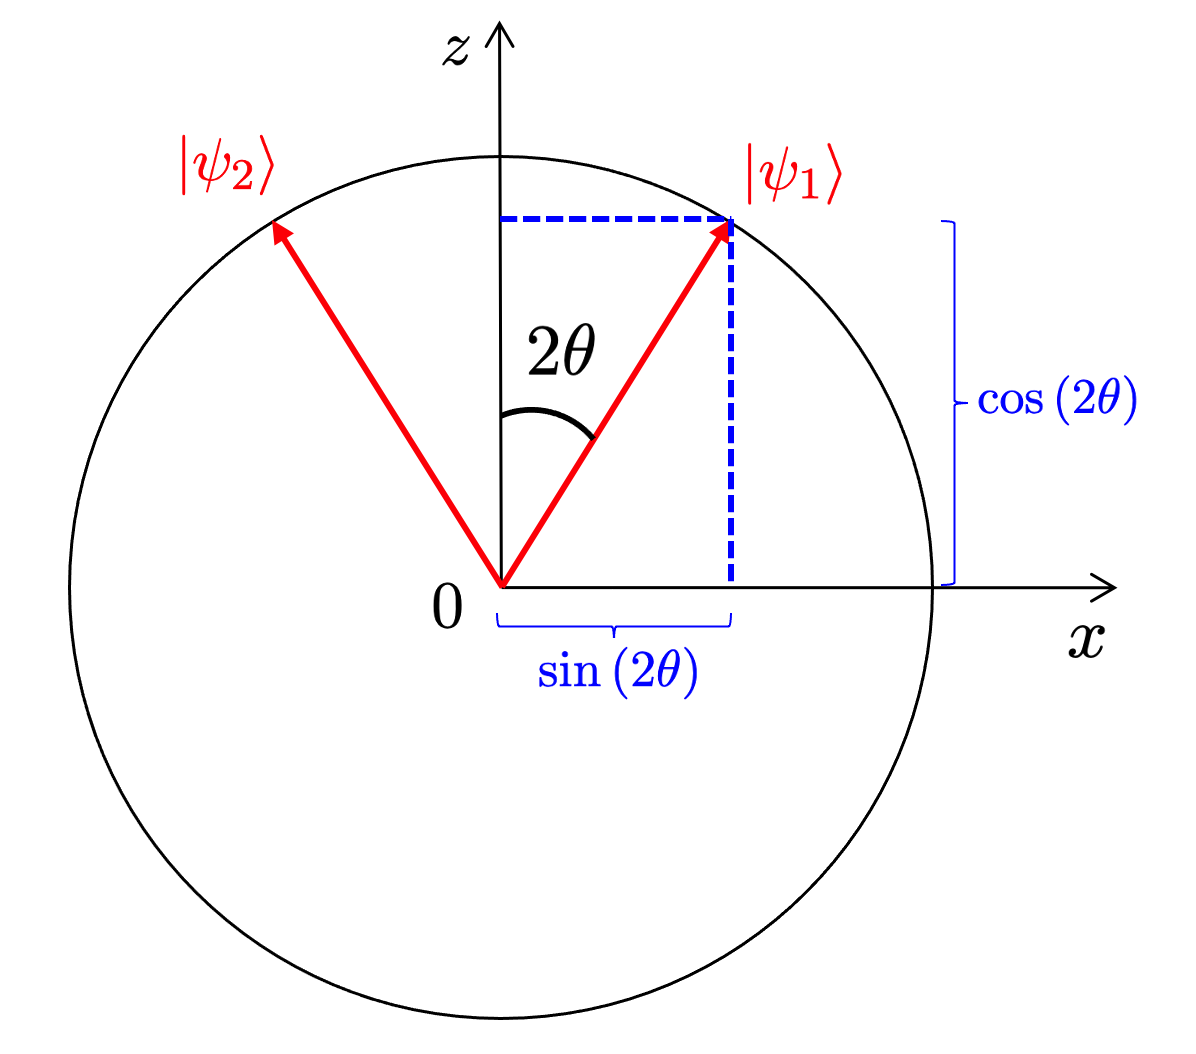
\includegraphics[width=0.48\linewidth]{images/Mixing_states_1.png}
    \caption{Discrete mixing of states on the surface of a Bloch sphere; only the $x-z$ plane of it is represented in this figure.}
    \label{fig:mix_states1}
\end{figure}

\begin{tcolorbox} [breakable, enhanced]
\textbf{Continuous mixing of states} \\
Consider a continuous mixing of states which are on the surface of the Bloch sphere, as shown in figure \ref{fig:mix_states2}; one of them is
\begin{align*}
    \ket{\psi(\theta,\varphi)} = \begin{pmatrix} \cos{\theta} \\ e^{i \varphi} \sin{\theta} \end{pmatrix}. 
\end{align*}
The density operator is 
\begin{align*}
    \rho &= \int \ket{\psi(\theta,\varphi)} \bra{\psi(\theta,\varphi)} \, dP(\varphi) = \\
    &= \int \ket{\psi(\theta,\varphi)} \bra{\psi(\theta,\varphi)} \, \frac{d \varphi}{2 \pi} = \\
    &= \int \begin{pmatrix} \cos^2{\theta} & e^{i \varphi} \cos{\theta} \sin{\theta} \\ \text{h.c.} & \sin^2{\theta} \end{pmatrix} \frac{d \varphi}{2 \pi} = \\
    &= \begin{pmatrix} \cos^2{\theta} & 0 \\ 0 & \sin^2{\theta} \end{pmatrix} 
\end{align*}
\end{tcolorbox}

\begin{figure}[H]
\centering
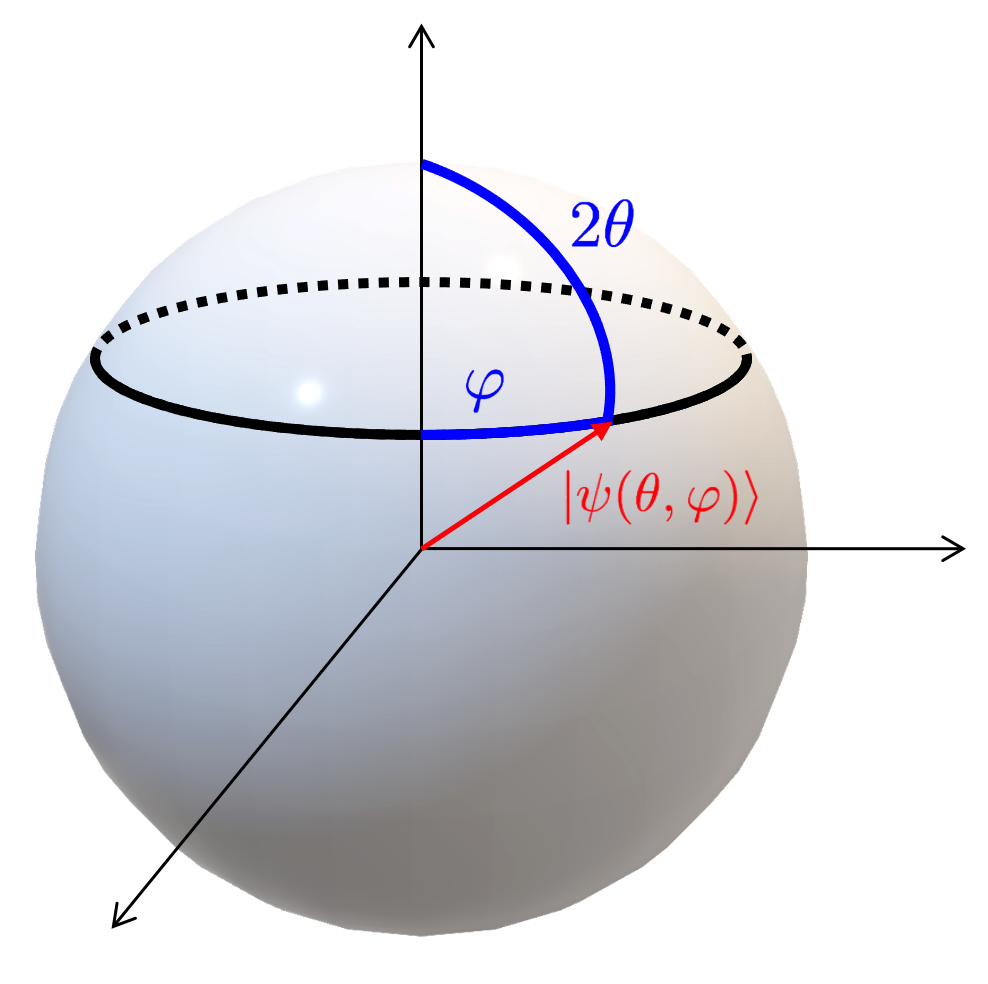
\includegraphics[width=0.45\linewidth]{images/Mixing_states_2.png}
    \caption{Continuous mixing of states on the surface of a Bloch sphere; for fixed values of $\theta$ and $\varphi$, the states $\ket{\psi(\theta,\varphi)}$ lie on a circumference.}
    \label{fig:mix_states2}
\end{figure}

\subsection{Reduced density operator}

In general, the interactions between the quantum system and the environment significantly change the dynamics of the system, therefore it is useful to develop a theoretical framework for treating them and for obtaining an accurate description of the dynamics of the system. Consider a bi-partition of a system into subsystem $A$ and subsystem $B$ which are associated to two Hilbert spaces with dimensions dim$_A$ and dim$_B$ and with sets of orthonormal bases $\ket{a_i}$ ($i = 1, ...,$ dim$_A$) and $\ket{b_j}$ ($j = 1, ...,$ dim$_B$), respectively. A generic element of the total system can be always written as 
\begin{align*}
    \ket{ab} = \sum_{i = 1}^{\text{dim}_A} \sum_{j = 1}^{\text{dim}_B} C_{ij} \ket{a_i}_A \otimes \ket{b_j}_B,
\end{align*}
where because of normalization 
\begin{align*}
    \sum_{i = 1}^{\text{dim}_A} \sum_{j = 1}^{\text{dim}_B} \abs{C_{ij}}^2 = 1.
\end{align*}
Consider now an observable of the full system $O_{AB} = O_A \otimes \mathbb{1}_B$ and evaluate the ensemble average:  
\begin{align*}
    \langle O_{AB} \rangle &= \text{Tr}[\left( O_A \otimes \mathbb{1}_B \right) \rho_{AB}] = \\
    &= \sum_a \sum_b (\bra{a}_A \otimes \bra{b}_B) \, \left[O_A \otimes \mathbb{1}_B \rho_{AB}\right] \, ( \ket{a}_A \otimes \ket{b}_B )= \\
    &= \sum_a \bra{a}_A O_A \left( \sum_b \bra{b}_B \rho_{AB} \ket{b}_B \right) \ket{a}_A = \\
    &= \sum_a \bra{a}_A O_A \rho_A \ket{a}_A = \\
    &= \text{Tr}[O_A \rho_A],
\end{align*}
where in the forth line the matrix operator $\rho_A$ is introduced
\begin{align}
    \rho_A = \sum_b \bra{b}_B \rho_{AB} \ket{b}_B = \text{Tr}_B[\rho_{AB}]
    \label{eq:rhoA}
\end{align}
and it is called \textit{reduced density operator} (or \emph{partial trace}) over system A. 
An analogous definition of $\rho_B$ can be obtained considering the observable $O_{AB} = \mathbb{1}_A \otimes O_B$:
\begin{align}
    \rho_B = \sum_a \bra{a}_A \rho_{AB} \ket{a}_A = \text{Tr}_A[\rho_{AB}].
    \label{eq:rhoB}
\end{align}
From these results, one can conclude that having $\rho_{AB}$ allows to obtain $\rho_A$ and $\rho_B$, but knowing $\rho_A$ and $\rho_B$ separately is not enough to reconstruct $\rho_{AB}$. Some examples relative to the evaluation of these quantities are given in the following. 

\begin{tcolorbox} [breakable, enhanced]
\textbf{Quantum correlated (entangled) state} \\ 
Consider the state $\ket{\Phi}$ and its associated density matrix
\begin{align*}
    \ket{\Phi} = \frac{1}{\sqrt{2}} \left( \ket{0 0 } + \ket{1 1} \right) \qquad \longrightarrow \qquad \rho = \frac{1}{2} \begin{pmatrix} 1 & 0 & 0 & 1 \\ 0 & 0 & 0 & 0 \\ 0 & 0 & 0 & 0 \\ 1 & 0 & 0 & 1 \end{pmatrix}.
\end{align*}
The reduced density operator $\rho_A$ is 
\begin{align*}
    \rho_A  = \frac{1}{2} \begin{pmatrix} 1 & 0 \\ 0 & 1 \end{pmatrix} = \frac{\mathbb{1}}{2}.
\end{align*}
\end{tcolorbox}

\begin{tcolorbox} [breakable, enhanced]
\textbf{Classical correlated state} \\ 
Consider the density matrix
\begin{align*}
    \rho = \frac{1}{2} \left( \ket{00} \bra{00} + \ket{11} \bra{11} \right) = \frac{1}{2} \begin{pmatrix} 1 & 0 & 0 & 0 \\ 0 & 0 & 0 & 0 \\ 0 & 0 & 0 & 0 \\ 0 & 0 & 0 & 1 \end{pmatrix}.
\end{align*}
Note that this state is not quantum entangled. The reduced density operator $\rho_A$ is 
\begin{align*}
    \rho_A = \frac{1}{2} \begin{pmatrix} 1 & 0 \\ 0 & 1 \end{pmatrix} = \frac{\mathbb{1}}{2}
\end{align*}
and it is the same obtained in the previous example despite the total density matrix is different.
\end{tcolorbox}

\begin{tcolorbox} [breakable, enhanced]
\textbf{Uncorrelated state} \\ 
Consider the density matrix
\begin{align*}
    \rho = \frac{1}{4} \left( \ket{00} \bra{00} + \ket{01} \bra{01} + \ket{10} \bra{10} +\ket{11} \bra{11} \right) = \frac{1}{4} \begin{pmatrix} 1 & 0 & 0 & 0 \\ 0 & 1 & 0 & 0 \\ 0 & 0 & 1 & 0 \\ 0 & 0 & 0 & 1 \end{pmatrix}.
\end{align*}
The reduced density operator $\rho_A$ is 
\begin{align*}
    \rho_A = \frac{1}{2} \begin{pmatrix} 1 & 0 \\ 0 & 1 \end{pmatrix} = \frac{\mathbb{1}}{2}
\end{align*}
which is equal to ones obtained previously. 
\end{tcolorbox}

From these examples, one can conclude that the partial trace hides (or deletes) the correlations between the elements of the subsystem $A$ and the elements of the subsystem $B$. \\


\section{System dynamics}
\label{sec:ME}

\subsection{Evolution of a closed quantum system}

For a given quantum system, the density operator at the initial and at the final instants of time are
\begin{align*}
    \rho_0 = \sum_\alpha p_\alpha \ket{\psi_\alpha} \bra{\psi_\alpha} \qquad \text{and} \qquad \rho(t) = \sum_\alpha p_\alpha \ket{\psi_\alpha(t)} \bra{\psi_\alpha(t)}.
\end{align*}
It is important to notice that every member evolves by itself (there is no interference) and therefore the probabilities $p_\alpha$ are static ($\dot{p}_\alpha = 0$). 
The evolution of the system is described by $\dot{\rho}(t)$ and from the previous relation 
\begin{align*}
    \dot{\rho}(t) &= \sum_\alpha p_\alpha \left( \ket{\dot{\psi}_\alpha(t)} \bra{\psi_\alpha(t)} + \ket{\psi_\alpha(t)} \bra{\dot{\psi}_\alpha(t)} \right) = \\
    &= \sum_\alpha p_\alpha \left( -\frac{i}{\hbar} H \ket{\psi_\alpha(t)} \bra{\psi_\alpha(t)} + \frac{i}{\hbar} \ket{\psi_\alpha(t)} \bra{\psi_\alpha(t)} H \right) = \\
    &= -\frac{i}{\hbar} H \left( \sum_\alpha p_\alpha \ket{\psi_\alpha(t)} \bra{\psi_\alpha(t)} \right) + \frac{i}{\hbar} \left( \sum_\alpha p_\alpha \ket{\psi_\alpha(t)} \bra{\psi_\alpha(t)} \right) H = \\
    &= \frac{i}{\hbar} [\rho,H].
\end{align*}
Some considerations about this result can be done:
\begin{itemize}
    \item The relation 
    \begin{equation}
        \label{eq:evol_rho}
        \dot{\rho}(t) = \frac{i}{\hbar} [\rho,H]
    \end{equation}
    is similar to the evolution equation for operators in the Heisenberg picture but with a different sign; this comes from the fact that the dynamics of the system is studied in the Schr\"odinger picture (the statevectors are functions of time). 
    \item If the mixture is made of eigenstates of $H$, it does not evolve in time (stationary system) because the commutator in (\ref{eq:evol_rho}) is null. 
\end{itemize}

\subsection{Evolution of an open quantum system}

In general, to describe the dynamics of an open quantum system, one needs to track the evolution of both the system and the bath together, but there are particular situations in which is possible to describe only the dynamics of the system without its coupling with the bath. This type of dynamics is called \textit{Born-Markovian dynamics} and it is based on the fact that, under certain requirements, the considered bath loses immediately memory of his interaction with the quantum system. This situation is schematize in the figure \ref{fig:sys_bath}. From the latter, it is possible to notice that:
\begin{itemize}
    \item the information proceeds only in one direction, from the system to the bath, it never comes back to the system;
    \item the bath needs to have an environment where to put acquired information, which is lost immediately.
\end{itemize}

\begin{figure}[H]
\centering
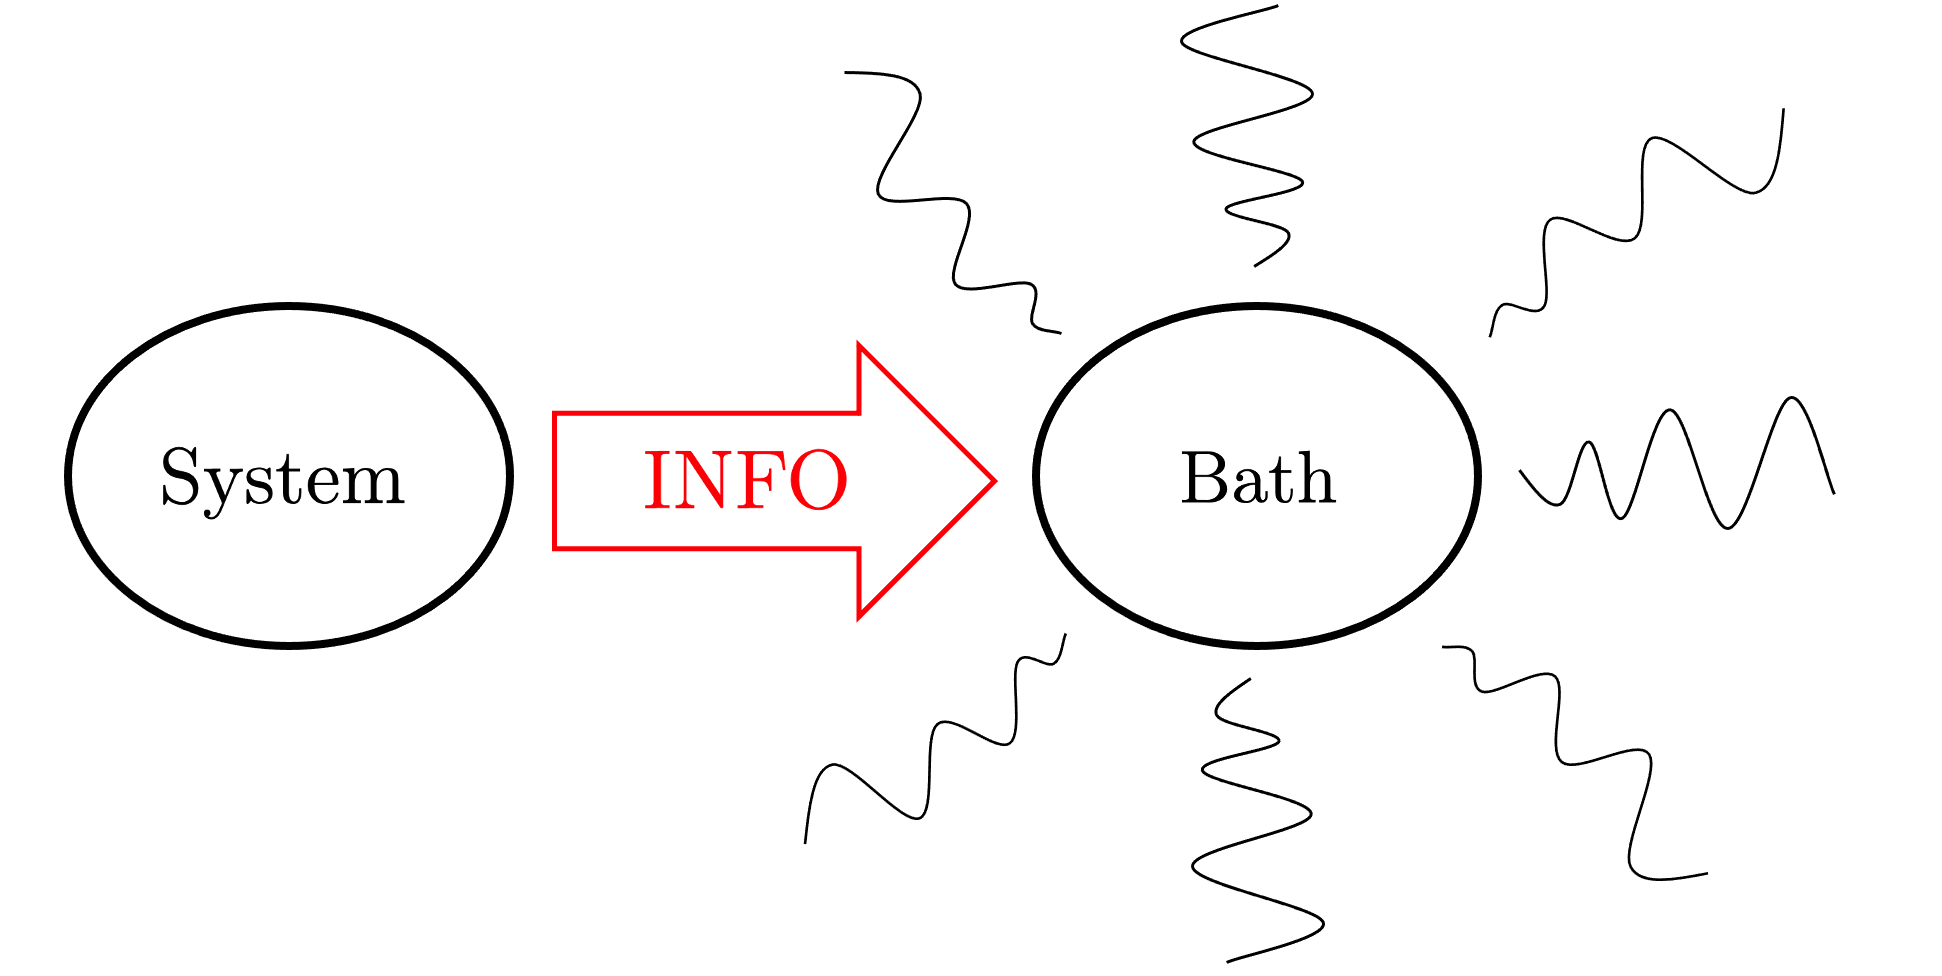
\includegraphics[width=0.68\linewidth]{images/System_and_Bath.png}
    \caption{System and bath in Born-Markovian dynamics; the information proceeds only in one direction, from the system to the bath, which immediately loses it.}
    \label{fig:sys_bath}
\end{figure}
Two physical requirements are necessary to realise this situation: 
\begin{enumerate}
    \item The bath has to be fast. If the system is described by the total Hamiltonian 
    \begin{align}
        H_\text{tot} = H_S + H_B + H_\text{int}
        \label{eq:HamLind}
    \end{align}
    and if each term is associate to a typical time $\tau_S$, $\tau_B$ and $\tau_\text{int}$, then the timescale separation must be
    \begin{align*}
        \tau_B \ll \tau_S  \lesssim \tau_\text{int}. 
    \end{align*}
    The first relation is required for the Born-Markovian dynamics, while the second one is useful for the quantum applications and technologies of the open system. 
    \item The bath has to be large. This means that dim$_S$ $\ll$ dim$_B$, since the bath must have space to store and forget information about the system. 
\end{enumerate}

In this framework, it is possible to describe the evolution of the density matrix for an open system described by a density matrix $\rho$ and with Hamiltonian $H$. The latter follows the \textit{Lindblad Master Equation}:
\begin{equation}
    \dot{\rho} = \frac{i}{\hbar} [\rho,H] + \sum_j \gamma_j \left( L_j \, \rho \,  L_j^\dagger - \frac{1}{2} \Bigl\{ L_j^\dagger L_j, \, \rho \Bigr\} \right),
    \label{eq:Lindblad}
\end{equation}
where:
\begin{itemize}
    \item $\rho$ and $H$ are operators associated only to the system ($H = H_S$ and $\rho = \rho_S$); 
    \item the first term in the right hand side describes the evolution of a closed quantum system, while the second term is associated to the coupling between the bath and the considered system;
    \item $\gamma_j$ is positive and has the dimension of s$^{-1}$, therefore it can be associated to a frequency (for instance, a rate of decay or a lifetime);
    \item $L_j$ are commonly called the \textit{Lindblad} or \textit{jump operators} of the system. 
\end{itemize}
The explicit expressions for $\gamma_\alpha$ and $L_\alpha$ can be obtained from the microscopic derivation of (\ref{eq:Lindblad}) which is presented in the following section. 

\subsection{Microscopic derivation of the Lindblad Master equation}

The starting point is the time-independent Hamiltonian in (\ref{eq:HamLind}) in which 
\begin{align*}
    H_S &= H_S \otimes \mathbb{1}_B, \\
    H_B &= \mathbb{1}_S \otimes H_B, \\
    H_\text{int} &= \sum_\alpha S_\alpha \otimes B_\alpha = \sum_\beta S_\beta^\dagger \otimes B_\beta^\dagger.
\end{align*}
The transformation 
\begin{align*}
    U(t) = \exp{\frac{i}{\hbar}t(H_S + H_B)}
\end{align*}
introduces $H'$ according to relation (\ref{eq:transfH}): 
\begin{align*}
    H'(t) &= U(t) H U^\dagger(t) - i \hbar U(t) \dot{U}^\dagger(t) = \\
    &= \exp{\frac{i}{\hbar}t(H_S + H_B)} (H_S + H_B + H_\text{int}) \exp{-\frac{i}{\hbar}t(H_S + H_B)} ~+ \\
    & \qquad - \exp{\frac{i}{\hbar}t(H_S + H_B)} (H_S + H_B) \exp{-\frac{i}{\hbar}t(H_S + H_B)} = \\
    &= \exp{\frac{i}{\hbar}t(H_S + H_B)} H_\text{int} \exp{-\frac{i}{\hbar}t(H_S + H_B)} = \\
    &= U(t) H_\text{int} U^\dagger(t),
\end{align*}
while $\rho(t) = \rho_{SB}(t)$ becomes
\begin{align*}
     \rho_{SB}'(t) = U(t) 
{\rho}_{SB}(t) U^\dagger(t).
\end{align*}
Therefore, equation (\ref{eq:evol_rho}) can be rewritten as 
\begin{align}
    \dot{\rho}'_{SB}(t) = \frac{i}{\hbar} [{\rho}'_{SB}(t), H'(t)].
    \label{eq:new_rho}
\end{align}
By integrating in time both sides of this relation, one obtains
\begin{align*}
    \rho_{SB}'(t) = \rho_{SB}'(0) + \frac{i}{\hbar} \int_0^t dt'[\rho_{SB}'(t'), H'(t')] 
\end{align*}
and by inserting this result in (\ref{eq:new_rho}) one can write an integro-differential equation:
\begin{align*}
    \dot{\rho}'_{SB}(t) = \frac{i}{\hbar} [{\rho}'_{SB}(0), H'(t)] - \frac{1}{\hbar^2} \int_0^t dt' \, [[\rho_{SB}'(t'), H'(t')], H'(t)] \equiv \triangle + \square.
\end{align*}
In the latter expression, the symbols $\triangle$ and $\square$ are introduced in order to indicate the commutator and the integral terms. \\
Now the trace over the bath density matrix of this equation is applied on the left and on the right; in order to develop the calculations, the contributions are studied separately. In particular:
\begin{itemize}
    \item In order to evaluate $\text{Tr}_B [ \triangle]$ the \textit{Born approximation} is used. The latter states that 
    \begin{align}
        \rho_{SB}(t) &= \rho_S(t) \otimes \rho_B(0), \\
        \rho'_{SB}(t) &= \rho'_S(t) \otimes \rho'_B(0) = \rho'_S(t) \otimes \rho_B(0).
    \end{align}
    and it means that the states of the system and of the bath are not correlated and that the latter does not evolve in time (stationary bath). Moreover, the following redefinitions of the parts of $H$ are considered: 
    \begin{align*}
        H_S \quad \longrightarrow \quad &H_S + \sum_\alpha S_\alpha \langle B_\alpha \rangle_B \\
        H_\text{int} \quad \longrightarrow \quad & H_\text{int} - \sum_\alpha S_\alpha \langle B_\alpha \rangle_B = \sum_\alpha S_\alpha \otimes \left(B_\alpha - \langle B_\alpha \rangle_B\right)
    \end{align*}
    Therefore
\begin{align*}
    \text{Tr}_B [\triangle] &= \frac{i}{\hbar} \text{Tr}_B \big( [\rho'_S(0) \otimes \rho_B(0),H'(t)]  \big) = \\
    &= \frac{i}{\hbar} \text{Tr}_B \left( \left[ \rho'_S(0) \otimes \rho_B(0),\sum_\alpha S'_\alpha \otimes (B'_\alpha - \langle B'_\alpha \rangle_B) \right] \right) = \\
    &= \frac{i}{\hbar} \sum_\alpha [\rho'_S(0),S'_\alpha(t)] \, \text{Tr}_B \Big( \rho_B(0) \left( B'_\alpha(t) - \langle B'_\alpha \rangle_B \right)\Big) = \\
    &= \frac{i}{\hbar} \sum_\alpha [\rho'_S(0),S'_\alpha(t)] \Big( \text{Tr}_B \left( \rho_B(0) B'_\alpha(t) \right) - \text{Tr}_B \left( \rho_B(0) \langle B'_\alpha \rangle_B \right) \Big) = \\
    &= \frac{i}{\hbar} \sum_\alpha [\rho'_S(0), S'_\alpha(t)] \left(\langle B'_\alpha \rangle_B - \langle B'_\alpha \rangle_B \right) = 0.
\end{align*}
From the second to the third line, some properties of the tensor product and of the trace operator are exploited (see Appendix A).
\item Also to evaluate 
\begin{align*}
     \text{Tr}_B [\square] &= \text{Tr}_B \left(- \frac{1}{\hbar^2} \int_0^t dt'\, [[\rho_{SB}'(t'), H'(t')], H'(t)] \right) = \\
     &= - \frac{1}{\hbar^2} \int_0^t dt' \, \text{Tr}_B \left([[\rho_{SB}'(t'), H'(t')], H'(t)] \right) = \\
    &= \frac{1}{\hbar^2} \int_0^t dt' \, \text{Tr}_B \left([[H'(t'),\rho_{SB}'(t')], H'(t)] \right)
\end{align*}
the Born approximation is used. In addition, the following expressions for $H'(t')$ and $H'(t)$ are inserted
\begin{align*}
    H'(t') &= \sum_\alpha S'_\alpha(t') \otimes B'_\alpha(t') \\
    H'(t) &= \sum_\beta S'^\dagger_\beta(t) \otimes B'^\dagger_\beta(t),
\end{align*}
in order to obtain 
\begin{align*}
    \text{Tr}_B [\square] = \frac{1}{\hbar^2} \int_0^t dt'\sum_{\alpha, \beta} S'_\alpha(t') \rho'_S(t') S'^\dagger_\beta(t) \, \text{Tr}_B \left[  B'_\alpha(t') \rho_B(0) B'^\dagger_\beta(t) \right] +\text{other 3 parts}.
\end{align*}
The trace in the previous expression can be evaluated explicitly: 
\begin{align*}
    \text{Tr}_B \left[  B'_\alpha(t') \rho_B(0) B'^\dagger_\beta(t) \right] &= \text{Tr}_B \left[ \rho_B(0) B'_\alpha(t')  B'^\dagger_\beta(t) \right] = \\
    &= \text{Tr}_B \left[ \rho_B(0) e^{i H_B t/\hbar} B_\beta^\dagger e^{-i H_B t/\hbar} e^{i H_B t'/\hbar} B_\alpha e^{-i H_B t'/\hbar} \right] = \\
    &= \text{Tr}_B \left[ \rho_B(0) e^{i H_B (t-t')/\hbar} B_\beta^\dagger e^{-i H_B (t-t')/\hbar} B_\alpha \right] = \\
    &= \text{Tr}_B \left[ \rho_B(0) {B'}_\beta^{\dagger}(t-t') B_\alpha \right] = \\
    &= \langle {B'}_\beta^\dagger(t-t') B_\alpha \rangle_B \equiv G_{\alpha \beta} (t-t')
\end{align*}
and hence
\begin{align}
    \text{Tr}_B [\square] =& \frac{1}{\hbar^2} \int_0^t dt' \sum_{\alpha, \, \beta} \bigg( G_{\alpha \beta} (t-t') \left( S'_\alpha(t') \rho'_S(t') S'^\dagger_\beta(t) - {S'}_\beta^\dagger(t) S'_\alpha(t') \rho'_S(t') \right) + \nonumber\\
    &+ G_{ \beta \alpha} (t'-t) \left( {S'}_\beta^\dagger(t) \rho'_S(t') S'_\alpha(t') - \rho'_S(t') S'_\alpha(t') {S'}_\beta^\dagger(t) \right) \bigg).
    \label{eq:cos}
\end{align}
At this point, another approximation to evaluate $G_{\alpha \beta}$ and $G_{\beta \alpha}$ is introduced; it is the \textit{Markov approximation} according to which
\begin{align*}
    G_{\alpha \beta} (t-t') = G_{\alpha \beta}(0) \delta(t-t') \qquad \text{and} \qquad   G_{\beta \alpha} (t'-t) = G_{\beta \alpha}(0) \delta(t'-t).
\end{align*}
It means that the time correlations of the bath decays are so fast that they can be approximated by a Dirac-$\delta$ function. Therefore
\begin{align*}
    \text{Tr}_B [\square] =& \frac{1}{\hbar^2} \sum_{\alpha, \, \beta} \bigg( G_{\alpha \beta} (0) \left( S'_\alpha(t) \rho'_S(t) S'_\beta(t) - {S'}_\beta^\dagger(t) S'_\alpha(t) \rho'_S(t) \right) ~+ \\
    &+ G_{ \beta \alpha} (0) \left( {S'}_\beta^\dagger(t) \rho'_S(t) S'_\alpha(t) - \rho'_S(t) S'_\alpha(t) {S'}_\beta^\dagger(t) \right) \bigg).
\end{align*}
By noticing that 
\begin{align*}
    G_{\alpha \beta}(0) &= \langle {B'}_\beta^\dagger(0) B'_\alpha(0) \rangle_B = \langle B_\beta^\dagger(0) B_\alpha(0) \rangle_B \\
    G_{\beta \alpha}(0) &= \langle {B'}_\alpha^\dagger(0) B'_\beta(0) \rangle_B = \langle B_\alpha^\dagger(0) B_\beta(0) \rangle_B \\
    G_{\alpha \beta}(0) &= G_{\beta \alpha}(0),
\end{align*}
the final result is 
\begin{align*}
    \text{Tr}_B [\square] &= \frac{1}{\hbar^2} \sum_{\alpha, \,\beta}  G_{\alpha \beta} (0) \bigg( 2 S'_\alpha(t) \rho'_S(t) S'_\beta(t) - {S'}_\beta^\dagger(t) S'_\alpha(t) \rho'_S(t) ~+ \\
    & \qquad - \rho'_S(t) {S'}_\beta^\dagger(t) S'_\alpha(t)  \bigg) = \\
    &= \frac{1}{\hbar^2} \sum_{\alpha, \,\beta}  G_{\alpha \beta} (0) \bigg( 2 S'_\alpha(t) \rho'_S(t) S'_\beta(t) - \Bigl\{\rho'_S(t), {S'}_\beta^\dagger(t) S'_\alpha(t)\Bigr\} \bigg)
\end{align*}
\item The left-hand part in the Born approximation gives 
    \begin{align*}
        \text{Tr}_B \left[ \dot{\rho}'_{SB}(t) \right] &= \text{Tr}_B \left[ \dot{\rho}'_{S}(t)  \otimes \rho_B(0) \right] +  \text{Tr}_B \left[ {\rho}'_{S}(t)  \otimes \dot{\rho}_B(0) \right] = \\
        &= \text{Tr}_B \left[ \dot{\rho}'_{S}(t) \right] \text{Tr}_B \left[\rho_B(0) \right] + \text{Tr}_B \left[ {\rho}'_{S}(t) \right] \text{Tr}_B \left[ \dot{\rho}_B(0) \right] = \\
        &= \text{Tr}_B \left[ \dot{\rho}'_{S}(t) \right] = \dot{\rho}'_{S}(t),
    \end{align*}
    since 
    \begin{align*}
        \text{Tr}_B \left[\rho_B(0) \right] = 1 \qquad \text{and} \qquad \text{Tr}_B \left[ \dot{\rho}_B(0) \right] = 0. 
    \end{align*}
\end{itemize}
Using these results, one obtains 
\begin{align*}
    \dot{\rho}'_{S}(t) = \frac{1}{\hbar^2} \sum_{\alpha,\, \beta} G_{\alpha \beta} (0) \bigg( 2 S'_\alpha(t) \rho'_S(t) S'_\beta(t) - \Bigl\{\rho'_S(t), {S'}_\beta^\dagger(t) S'_\alpha(t) \Bigr\} \bigg).
\end{align*}
The last step consists in returning to the original frame. The explicit calculations are omitted and the final result is obtained multiplying on the left by $\exp{-i \hbar H_S/t}$ and on the right by $\exp{i \hbar H_S/t}$: 
\begin{equation}
    \dot{\rho}_{S}(t) = \frac{i}{\hbar} [\rho_S(t),H_S] + \frac{1}{\hbar^2} \sum_{\alpha, \, \beta} \bigg( 2 S_\alpha \rho_S(t) S_\beta - \Bigl\{\rho_S(t), S_\beta^\dagger S_\alpha \Bigr\} \bigg). 
    \label{eq:genLindblad}
\end{equation}
This the Lindblad Master equation in general form. In order to obtain the expression in (\ref{eq:Lindblad}), one should notice that the matrix with elements $G_{\alpha \beta}$ is positive definite and that it can be diagonalized with a proper change of basis like
\begin{align*}
    G_{\alpha \beta} = T_{j \alpha } \gamma_j T_{j \beta } \qquad \text{with} \qquad \gamma_j \leq 0. 
\end{align*}
Moreover, one can introduce the operators 
\begin{align*}
    L_j \equiv \sqrt{2} \sum_{\alpha} T_{j \alpha} S_\alpha 
\end{align*}
and rewrite (\ref{eq:genLindblad}) as
\begin{align*}
    \dot{\rho}_S = \frac{i}{\hbar} [\rho_S(t),H] + \sum_j \gamma_j \left( L_j \, \rho_S(t) \,  L_j^\dagger - \frac{1}{2} \Bigl\{ L_j^\dagger L_j, \, \rho_S(t) \Bigr\} \right),
\end{align*}


\subsection{Applications of the Lindblad Master equation}

\begin{tcolorbox} [breakable, enhanced]
\textbf{Decay} \\ 
Consider a two-level system described by the Hamiltonian 
\begin{align*}
    H = \hbar \omega \ket{e}\bra{e} = \hbar \omega \begin{pmatrix} 0 & 0 \\ 0 & 1 \end{pmatrix}
\end{align*}
and take a single Lindblad operator $L = \ket{g}\bra{e}$. Therefore $\gamma$ is equal to the rate associated to the jump to the ground state $\ket{g}$. \\
The generic expression of the density operator is 
\begin{align}
    \rho(t) = \begin{pmatrix} a(t) & b(t) \\ b^*(t) & c(t) \end{pmatrix} \quad \text{with} \quad \begin{cases} a(t) + c(t) = 1 & \text{(trace-less matrix)} \\ \abs{b(t)}^2 \leq a(t) \, c(t) & \text{(positivity condition)} \end{cases}
    \label{eq:gen_rho}
\end{align}
Equation (\ref{eq:Lindblad}) becomes 
\begin{align*}
    \dot{\rho}(t) = -\frac{i}{\hbar} H \rho(t) + \frac{i}{\hbar} \rho(t) H + \gamma L \rho(t) L^\dagger - \frac{\gamma}{2} L^\dagger L \rho(t) - \frac{\gamma}{2} \rho L L^\dagger 
\end{align*}
and inserting the matrices for $H$ and $\rho(t)$
\begin{align*}
    \begin{pmatrix} \dot{a}(t) & \dot{b}(t) \\ \dot{b}^*(t) & \dot{c}(t) \end{pmatrix} =&~ i \omega \left( \begin{pmatrix} 0 & b(t) \\ 0 & c(t) \end{pmatrix} - \begin{pmatrix} 0 & 0 \\ b^*(t) & c(t) \end{pmatrix} \right) + \\
    & + \gamma \left( \begin{pmatrix} c(t) & 0 \\ 0 & 0 \end{pmatrix} - \frac{1}{2} \begin{pmatrix} 0 & 0 \\ b^*(t) & c(t) \end{pmatrix} - \frac{1}{2} \begin{pmatrix} 0 & b(t) \\ 0 & c(t) \end{pmatrix} \right)
\end{align*}
it is possible to write differential equations for $b(t)$ and $c(t)$
\begin{align*}
    \begin{cases}
    \dot{b}(t) = \displaystyle \left( i \omega - \dfrac{\gamma}{2}\right) b(t) \\
    \dot{c}(t) = -\gamma \, c(t) 
    \end{cases}
\end{align*}
Therefore from (\ref{eq:gen_rho}), 
\begin{align*}
    \rho(t) = \begin{pmatrix} 1-c_0 \, e^{-\gamma t} & b_0 \, e^{t(i\omega - \gamma/2)} \\ \text{c.c.} & c_0 \, e^{-\gamma t} \end{pmatrix},
\end{align*}
where $a_0$, $b_0$ in $c_0$ are the matrix elements at the initial time. One can notice that the expression for $b(t)$ describes oscillations with frequency $\omega$, while the one for $c(t)$ represents an exponential decay with rate $\gamma$. Some expectation values can be evaluated:
\begin{align*}
    \langle \sigma^z \rangle &= a(t) - c(t) = 1 - 2 c_0 \, e^{- \gamma t} \\
    \langle \sigma^x \rangle &= b(t) + b^*(t) = e^{-\gamma t /2} \, \real{\left(b_0 \, e^{i \omega t }\right)} = e^{-\gamma t /2} b_0 \cos{(\omega t)}  \qquad (b_0 \in \mathbb{R})
\end{align*}
and they can be use to visualize the evolution. 
\begin{figure}[H]
\centering
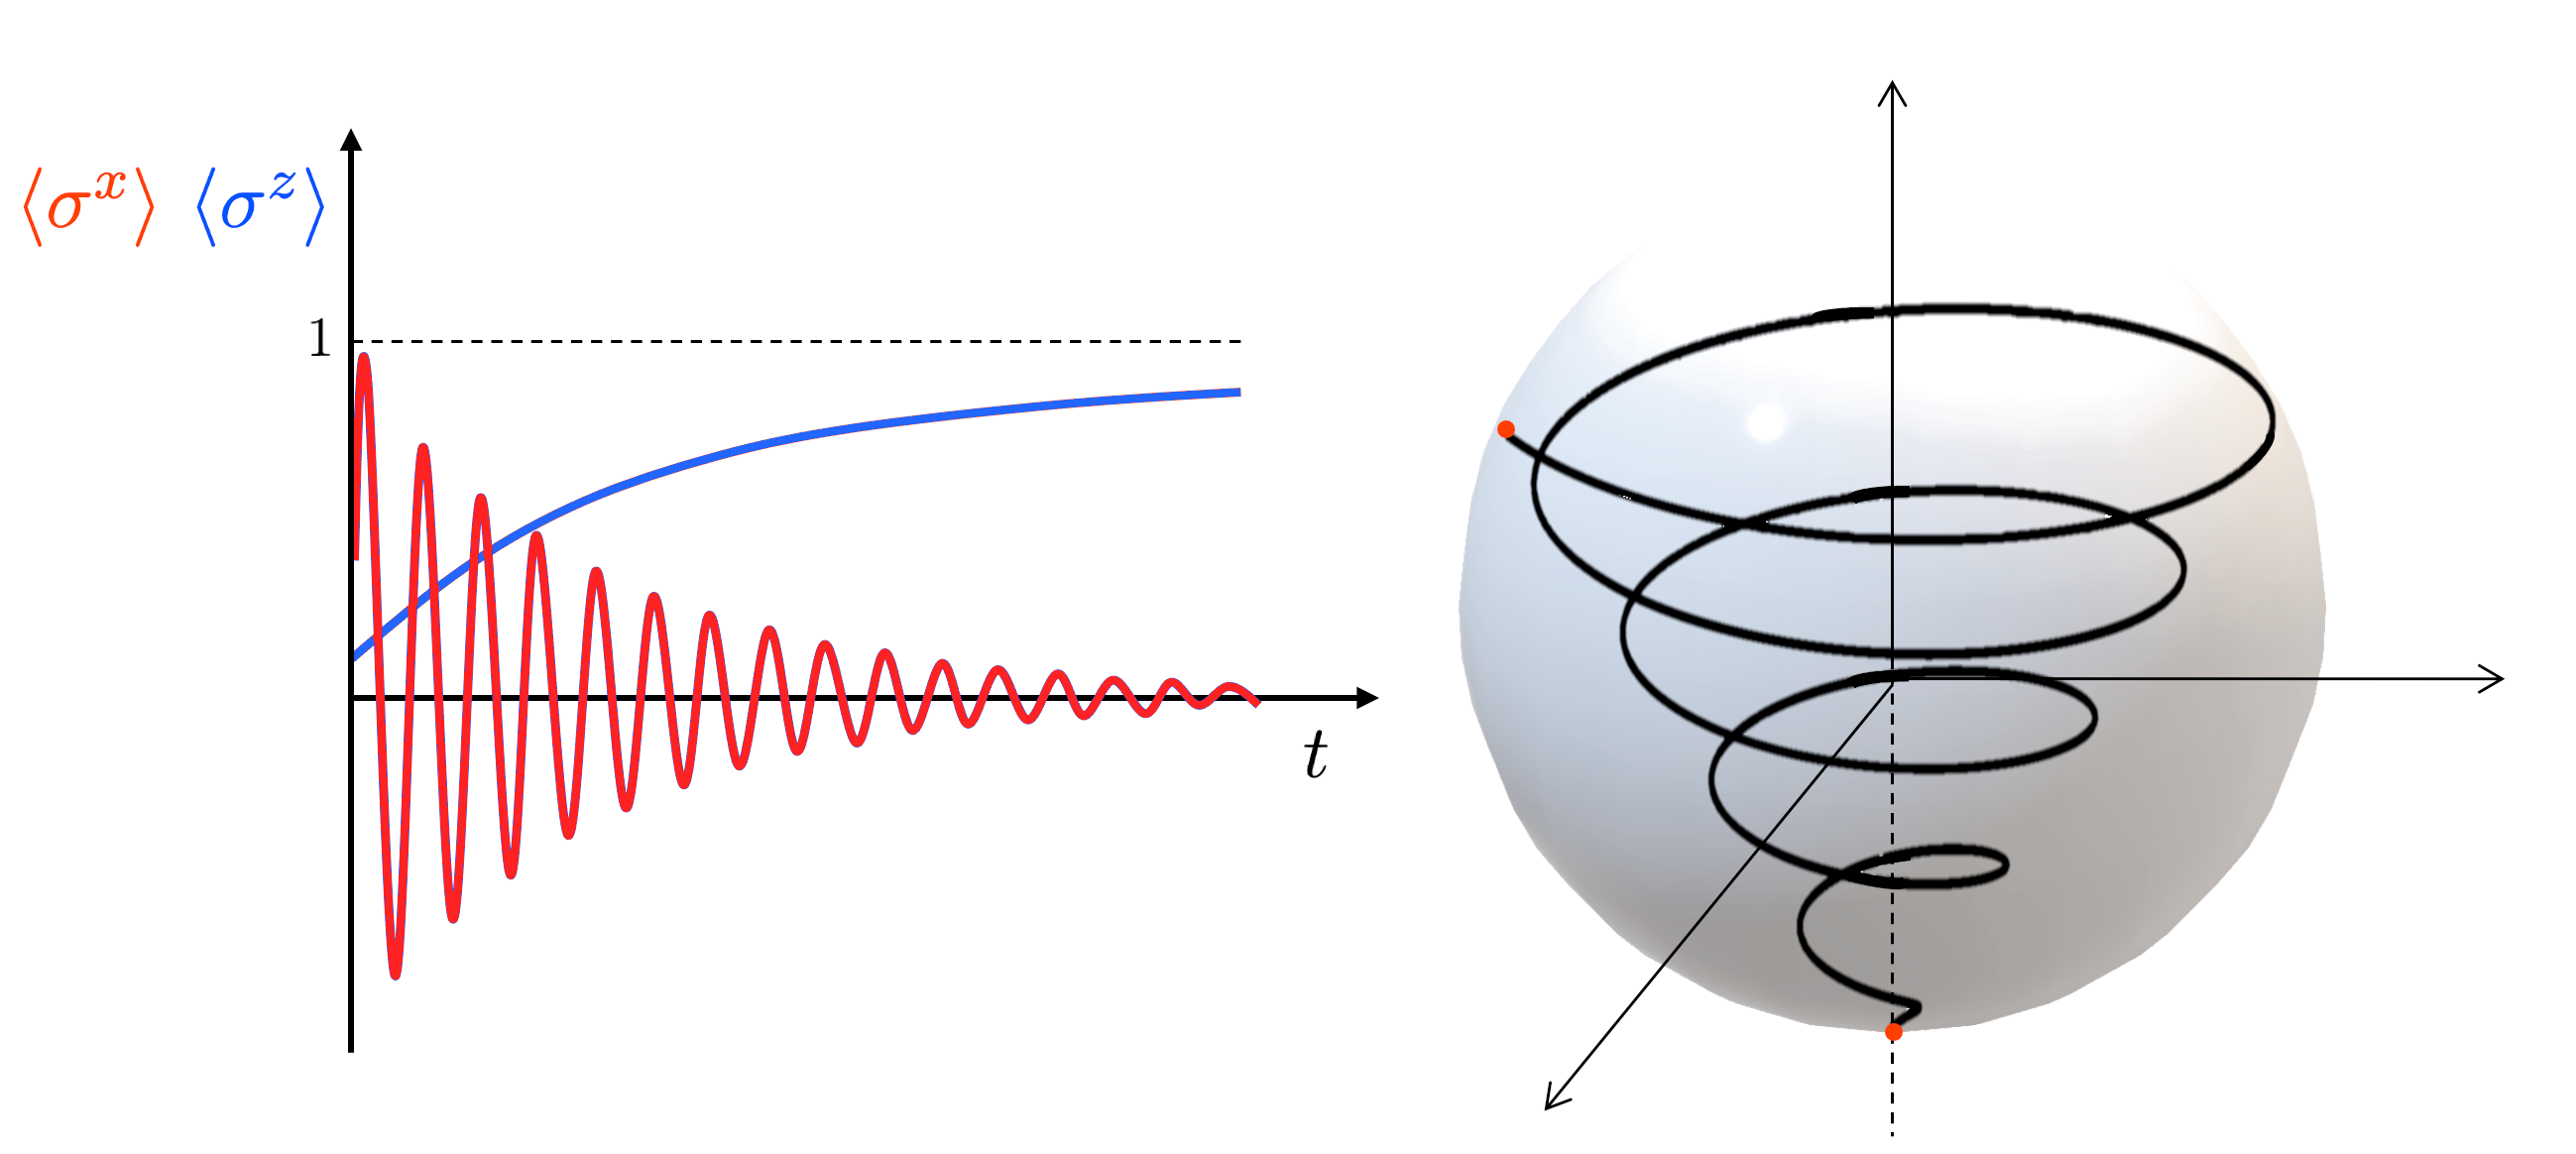
\includegraphics[width=0.87\linewidth]{images/Decay.png}
    \caption{Decay of a mixed state after the action of the Lindblad operator $L = \ket{g}\bra{e}$; the oscillation frequency of $\langle \sigma^x \rangle$ is equal to $\omega$, while the exponential decay of $\langle \sigma^z \rangle$ it is characterized by a frequency $\gamma$ (the same of $L$).}
    \label{fig:decay}
\end{figure}

Moreover, in the limit $t \to \infty$ the matrix operator becomes 
\begin{align*}
    \rho_\infty = \begin{pmatrix} 1 & 0 \\ 0 & 0 \end{pmatrix} = \ket{g}\bra{g}
\end{align*}
and it describes a steady state.
\end{tcolorbox}



\begin{tcolorbox} [breakable, enhanced]
\textbf{Dephasing (first part)} \\ 
Consider a two-level system descrived by the Hamiltonian 
\begin{align*}
    H = \hbar \omega \ket{e}\bra{e} = \hbar \omega \begin{pmatrix} 0 & 0 \\ 0 & 1 \end{pmatrix} 
\end{align*}
and take a single Lindblad operator $L = \ket{e}\bra{e}$. Therefore $\gamma$ is equal to the rate associated to the phase flip of the state. Also in this case, one can start from the generic expression of the density operator (\ref{eq:gen_rho}) in order to rewrite equation (\ref{eq:Lindblad}):
\begin{align*}
    \begin{pmatrix} \dot{a}(t) & \dot{b}(t) \\ \dot{b}^*(t) & \dot{c}(t) \end{pmatrix} =&~ i \omega \begin{pmatrix} 0 & b(t) \\ b^*(t) & 0 \end{pmatrix} + \gamma \Bigg( \begin{pmatrix} 0 & 0 \\ 0 & c(t) \end{pmatrix} + \\
    & - \frac{1}{2} \begin{pmatrix} 0 & b(t) \\ 0 & c(t) \end{pmatrix} - \frac{1}{2} \begin{pmatrix} 0 & 0 \\ b^*(t) & c(t) \end{pmatrix} \Bigg)
\end{align*}
and to obtain the differential equations for $b(t)$ and $c(t)$
\begin{align*}
    \begin{cases}
    \dot{b}(t) = \displaystyle \left( i \omega - \dfrac{\gamma}{2}\right) b(t) \\
    \dot{c}(t) = 0 
    \end{cases}
\end{align*}
Therefore
\begin{align*}
    \rho(t) = \begin{pmatrix} 1-c_0 & b_0 \, e^{t(i\omega - \gamma/2)} \\ \text{c.c.} & c_0 \end{pmatrix},
\end{align*}
where $a_0$, $b_0$ in $c_0$ are the matrix elements at the initial time. Some expectation values can be evaluated:
\begin{align*}
    \langle \sigma^z \rangle &= a(t) - c(t) = 1 - 2 c_0 \qquad (\text{conserved quantity}), \\
    \langle \sigma^x \rangle &= b(t) + b^*(t) = e^{-\gamma t /2} \, \real{\left(b_0 \, e^{i \omega t }\right)} = e^{-\gamma t /2} b_0 \cos{(\omega t)}  \qquad (b_0 \in \mathbb{R}),
\end{align*}
while in the limit $t \to \infty$ the matrix operator becomes
\begin{align*}
    \rho_\infty = \begin{pmatrix} 1-c_0 & 0 \\ 0 & c_0 \end{pmatrix},
\end{align*}
which describes a non-unique steady state. 
\end{tcolorbox}

\begin{figure}[H]
\centering
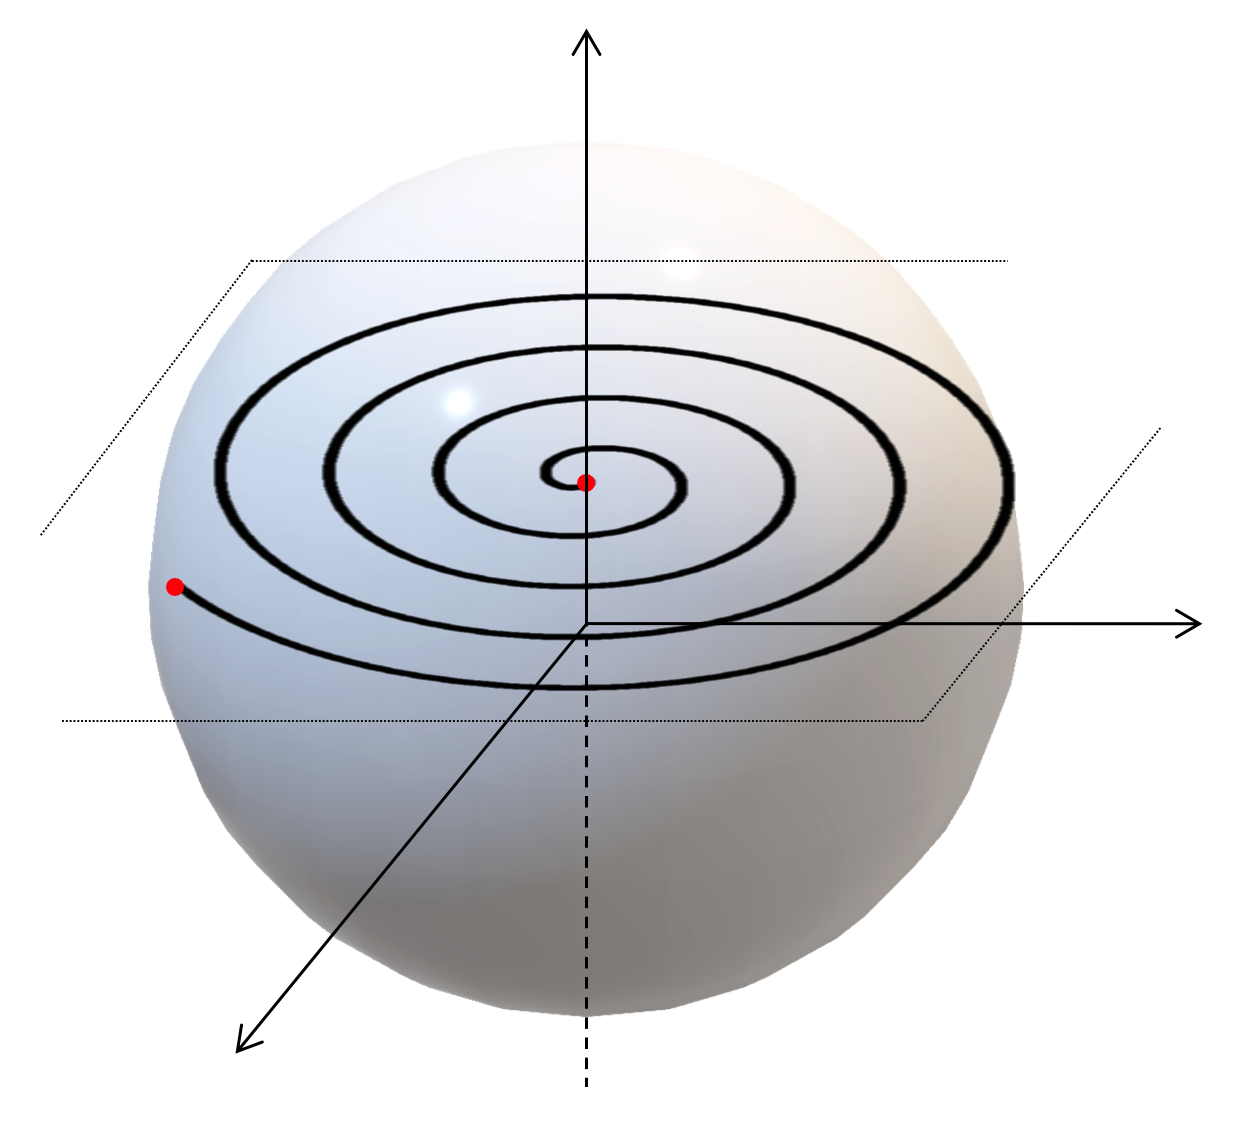
\includegraphics[width=0.47\linewidth]{images/Dephasing.png}
    \caption{Dephasing of a mixed state after the action of the Lindblad operator $L = \ket{e}\bra{e}$; the oscillation frequency of $\langle \sigma^x \rangle$ is equal to $\omega$.}
    \label{fig:dephasing}
\end{figure}

In both the presented examples, the entropy is not a precise indicator of the information of the system. Indeed, through explicit calculation, it is possible to show that in the second case $\mathcal{S}$ increases more with the respect to the first one, but the loss of information is reduced, since the evolution plane is known. 

\begin{tcolorbox} [breakable, enhanced]
\textbf{Dephasing (second part)} \\ 
Consider a two-level system described by the Hamiltonian
\begin{align*}
    H = \hbar \omega \ket{e}\bra{e} = \hbar \omega \begin{pmatrix} 0 & 0 \\ 0 & 1 \end{pmatrix} 
\end{align*}
and consider it subject to a classical noise (and not coupled to a bath). Therefore $\omega$ is a fixed random variable extracted from a probability distribution with probability density given by a Cauchy-Lorentzian distribution
\begin{align*}
    \frac{d p}{d \omega} = \frac{1}{\pi} \frac{\gamma}{(\omega - \omega_0)^2 + \gamma^2}. 
\end{align*}
With a procedure analogous to the one presented in the previous example, the density operator for a fixed valued of $\omega$ is
\begin{align*}
    \rho_\omega(t) = \begin{pmatrix} 1-c_0 & b_0 \, e^{i\omega t} \\ b_0^* \, e^{- i\omega t} & c_0 \end{pmatrix},
\end{align*}
while the one for the Hamiltonian ensemble is 
\begin{align*}
    \rho_\text{ensemble}(t) &= \int \rho_\omega(t) \, dp(\omega) = \bigintsss \begin{pmatrix} 1-c_0 & b_0 \, e^{i\omega t} \\ b_0^* \, e^{- i\omega t} & c_0 \end{pmatrix} \frac{dp}{d\omega} d\omega = \\
    &= \begin{pmatrix} 1-c_0 & b_0 \displaystyle \int e^{i\omega t} \dfrac{dp}{d\omega} d \omega \\ b_0^* \displaystyle \int e^{-i\omega t} \dfrac{dp}{d\omega} d \omega & c_0 \end{pmatrix} = \\
    &=  \begin{pmatrix} 1-c_0 & b_0 \, e^{(i\omega_0-\gamma) t} \\ \text{c.c.} & c_0 \end{pmatrix},
\end{align*}
where the last equation comes from 
\begin{align*}
    \int_{-\infty}^{+\infty} \frac{d \omega}{\pi} \frac{\gamma e^{i \omega t}}{(\omega - \omega_0)^2 + \gamma^2} = e^{i \omega_0 t - \gamma \abs{t}}.
\end{align*}
It is important to notice that the result for $\rho_\text{ensemble}$ is equivalent to the one obtained in the previous example for an open system coupled to a bath: Born-Markovian dynamics also models some forms of classical noise. 
\end{tcolorbox}

\subsection{Formal integration of the Lindblad Master equation}

The formal integration of the Lindblad Master equation can be performed by means of a \textit{vectorialization} procedure. In the first place, one can introduce the \textit{Liouvillian super-operator} (a super-operator is just an operator acting on an operator)
\begin{equation}
    \mathcal{L}(\rho) \equiv \frac{i}{\hbar} [\rho,H] + \sum_j \gamma_j \left( L_j \, \rho \,  L_j^\dagger - \frac{1}{2} \Bigl\{ L_j^\dagger L_j, \, \rho \Bigr\} \right),
    \label{eq:Liouvillian}
\end{equation}
and one can notice that equation (\ref{eq:Lindblad}) is equivalent to the Schr\"odinger equation, because $\mathcal{L}$ is a first order (in time) and linear operator ($\mathcal{L}(\rho_1 + \rho_2) = \mathcal{L}(\rho_1) + \mathcal{L}(\rho_2)$), and one is able to formally integrate it. In order to do this, some other steps are necessary and they constitute the \textit{Choi-Jamiolkowski isomorphism} (or vectorization). The latter can be captured by the relation
\begin{align}
    \ket{i}\bra{j} \quad \longrightarrow \quad \ket{j} \otimes \ket{i} \equiv \ket{ij}\rangle
    \label{eq:Choi}
\end{align}
and therefore one can think about an outer product (which has two indices) as being just a vector (with one index). In addition, using (\ref{eq:Choi}) the density matrix $\rho$ (with dimension dim$_H$ x dim$_H$) is transformed into the super-vector $\ket{\rho}\rangle$ (with dimension dim$^2_H$ x 1): 
\begin{align*}
        \rho = \sum_{i, \, j} \rho_{ij} \ket{i}\bra{j} \quad \longrightarrow \quad \ket{\rho}\rangle = \sum_{i, \, j} \rho_{ij} \ket{ij}\rangle.
\end{align*}
From a matrix point of view, this operation is the same as stacking columns of a matrix:
\begin{align}
    M = \begin{pmatrix} a & b \\ c & d \end{pmatrix}  \quad \longrightarrow \quad \ket{M}\rangle = \begin{pmatrix} a \\ b \\ c \\ d \end{pmatrix}.
    \label{eq:matrixtransf}
\end{align}
This trick is very useful due to two particular properties:
\begin{enumerate}
    \item The first one is related to the \textit{Hilbert-Schmidt inner product} (which satisfies all the properties of an inner product and therefore is analogous to $\braket{i}{j}$), defined as
    \begin{align*}
        \left( A,B\right)_{\mathcal{HS}} \equiv \langle \braket{A}{B} \rangle = \text{Tr}\left[ A^\dagger B \right].
    \end{align*}
    From this relation and (\ref{eq:matrixtransf}), one can intuitively guess that 
    \begin{align}
         \text{Tr}\left[ A^\dagger B \right] = \ket{A}\rangle^\dagger \ket{B}\rangle =  \langle \braket{A}{B} \rangle, 
         \label{eq:traceVect}
    \end{align}
    that is just the inner product between two vectors. 
    \item The second property is 
    \begin{align}
        \ket{A\, B\, C}\rangle = \left( C^t \otimes A \right) \ket{B}\rangle.
    \end{align}
    The usefulness of this relation lies in the fact that it provides a recipe to write super-operator products in the form of a big matrix times $\ket{{\rho}}\rangle$:
    \begin{align*}
        \ket{A{\rho}}\rangle = \ket{A \, {\rho} \, \mathbb{1}}\rangle = (\mathbb{1} \otimes A) \ket{{\rho}}\rangle 
    \end{align*}
\end{enumerate}
With these properties it is possible to rewrite the Liouvillian super-operator $\mathcal{L}$ as a super-matrix $\hat{\hat{\mathcal{L}}}$, indeed the two terms of (\ref{eq:Liouvillian}) become:
\begin{align*}
    \ket{\frac{i}{\hbar} [\rho,H]}\biggr\rangle &= -\frac{i}{\hbar} \left( \mathbb{1} \otimes H - H^t \otimes \mathbb{1} \right) \ket{\rho}\rangle,\\
    \ket{ L_j \, \rho \,  L_j^\dagger - \frac{1}{2} \Bigl\{ L_j^\dagger L_j, \, \rho \Bigr\} } \biggr\rangle &= \left( L_j^t \otimes L_j - \frac{1}{2} \mathbb{1} \otimes L_j^\dagger L_j - \frac{1}{2} (L_j^\dagger L_j)^t \otimes \mathbb{1} \right) \ket{\rho}\rangle.
\end{align*}
Therefore, the original Lindblad Master equation becomes 
\begin{align}
    \ket{\dot{\rho}}\rangle = \hat{\hat{\mathcal{L}}} \ket{{\rho}}\rangle
    \label{eq:LindbladVect}
\end{align}
with 
\begin{align}
    \hat{\hat{\mathcal{L}}} = -\frac{i}{\hbar} \left( \mathbb{1} \otimes H - H^t \otimes \mathbb{1} \right) + \sum_j \gamma_j \left( L_j^t \otimes L_j - \frac{1}{2} \mathbb{1} \otimes L_j^\dagger L_j - \frac{1}{2} (L_j^\dagger L_j)^t \otimes \mathbb{1} \right) 
\end{align}
Equation (\ref{eq:LindbladVect}) is similar to the Schr\"odinger equation, therefore one can suppose a solution of the form
\begin{align}
    \ket{\rho(t)}\rangle = \exp{\hat{\hat{\mathcal{L}}}t} \ket{\rho_0}\rangle. 
\end{align}
However $\hat{\hat{\mathcal{L}}}$ is not Hermitian and hence it is not guaranteed that it can be diagonalized. Nevertheless, if it is possible to find a matrix transformation $X$ such that $\hat{\hat{\mathcal{L}}} = X D X^\dagger$ (with $D$ diagonal matrix), then the solution is 
\begin{align}
    \ket{\rho(t)}\rangle = X e^{Dt} X^{-1}\ket{\rho_0}\rangle. 
\end{align}
Some final comments can be done:
\begin{itemize}
    \item The matrix $X$ is not an orthonormal matrix and its elements can be complex; in order to consider only physical solutions (in this case these that do not explodes exponentially), one must impose that $\forall d_j \in D$, $\real{(d_j)} \leq 0$.
    \item The steady state is
    \begin{align*}
        \ket{\dot{\rho}_{SS}}\rangle = 0 \qquad \Longleftrightarrow \qquad \hat{\hat{\mathcal{L}}} \ket{{\rho_{SS}}}\rangle = 0
    \end{align*}
    and hence $\ket{{\rho_{SS}}}\rangle$ must be in the kernel of $\hat{\hat{\mathcal{L}}}$. 
    \item Not all the eigenvectors are density matrix with unitary trace. In order to verify this, notice that the solutions of the eigen(super-)value equation $\hat{\hat{\mathcal{L}}} \ket{\Bar{\rho}}\rangle = \lambda \ket{\Bar{\rho}}\rangle$ associated to (\ref{eq:LindbladVect}) can be written as $\ket{\Bar{\rho}(t)}\rangle = e^{\lambda t} \ket{\Bar{\rho}_0}\rangle$; moreover, equation (\ref{eq:LindbladVect}) preserves the norm, indeed form (\ref{eq:traceVect})
    \begin{align*}
        \text{Tr}[\rho] = \text{Tr}[\mathbb{1} \, \rho] =  \text{Tr}[\mathbb{1}^\dagger \rho] = \langle \braket{\mathbb{1}}{\rho}\rangle = 1,
    \end{align*}
    therefore, if $\real{(\lambda)} < 0$, 
    \begin{align*}
        \text{Tr}[{\Bar{\rho}}_0] = \text{Tr}[\Bar{\rho}] = e^{\lambda t} \text{Tr}[{\Bar{\rho}_0}] \qquad \implies \qquad \text{Tr}[{\Bar{\rho}}] =  \text{Tr}[\Bar{\rho}] = 0.
    \end{align*}
    This means that all decaying eigen(super-)vectors are traceless and are not density matrices. 
\end{itemize}


\chapter{Quantization of light}
% -----------------------------------------------------------
%
%  CHAPTER 4  of Quantum information with atoms and photons
%
%  written by Ilaria Delbono + others,Jan 2023
% -----------------------------------------------------------


Electromagnetic waves and, in turn, light come from the coexistence of an electric field $\vec{E}=\vec{E}(\Vec{x},t)$ and a magnetic field $\vec{B}=\vec{B}(\Vec{x},t)$. In vacuum and in absence of sources, they are described by 
the following  Maxwell's Equations: 

\begin{align}
    \vec{\nabla} \cdot \vec{E} &=0, \label{eq:ME1}\\
    \vec{\nabla}\cdot \vec{B} &=0,\label{eq:ME2} \\
    \vec{\nabla}\times\vec{E} &=-\frac{\partial \vec{B}}{\partial t}, \label{eq:ME3}\\
    \vec{\nabla}\times\vec{B} &=\frac{1}{c^2} \frac{\partial \vec{E}}{\partial t}, \label{eq:ME4}
\end{align}
where $c^2 = \varepsilon_0 \mu_0$. 
From these equations, it is possible to find that the electric and magnetic fields satisfy the \textit{Wave Equation}:
\begin{align}
         \left(\nabla^{2}-\frac{\partial^{2}}{\partial t^{2}}\right)\vec{E} &= 0, \\
         \left(\nabla^{2}-\frac{\partial^{2}}{\partial t^{2}}\right)\vec{B} &= 0.
\end{align}
The solutions are
 \begin{equation}
     \vec{E}(\vec{x},t)=\vec{E}_{0} \, e^{i(\vec{k} \cdot \vec{r}-\omega t)} \qquad \text{and} \qquad 
     \vec{B}(\vec{x},t)=\vec{B}_0 \, e^{i(\vec{k} \cdot \vec{r}-\omega t)}. 
 \end{equation}

\section{First Quantization}
\subsection{Electromagnetic potentials and Coulomb gauge}
\label{subsec:3.1.1}
The expressions for $\vec{E}$ and $\vec{B}$ can be derived from a scalar potential $\phi$ and a vector potential $\vec{A}$: 
\begin{equation}
    \vec{E}=-\frac{\partial \vec{A}}{\partial t} - \vec{\nabla}\phi \qquad \text{and} \qquad \vec{B}=\vec{\nabla}\times\vec{A}. 
    \label{eq:empot}
\end{equation}
Maxwell's equations are invariant under the transformations
\begin{align*}
    \phi ~~\longrightarrow ~~ \phi - \frac{\partial f}{\partial t}  \qquad \text{and} \qquad \vec{A}~~\longrightarrow ~~ \vec{A} + \vec{\nabla} f, 
\end{align*}
which are defined for a generic function $f(\vec{r},t)$. This arbitrariness in the definition of $\phi$ and $\vec{A}$ is called \textit{gauge invariance}. In absence of source, it is useful to work with the \textit{Coulomb gauge}: 
\begin{align}
    \phi=0 \qquad \text{and} \qquad \vec{\nabla}\cdot \vec{A}=0. 
\end{align}
This choice allows to deduce the equation of motion for $\vec{A}$. Starting from (\ref{eq:ME4}) and using (\ref{eq:empot}), the left-hand side and the right-hand side become: 
\begin{align}
    \vec{\nabla}\times\vec{B}&=\vec{\nabla}\times(\vec{\nabla}\times\vec{A}) =\vec{\nabla}(\vec{\nabla}\cdot \vec{A})-\nabla^{2}\vec{A} = -\nabla^{2}\vec{A}, \\
    \frac{1}{c^{2}}\frac{\partial \vec{E}}{\partial t} &= -\frac{1}{c^{2}}\frac{\partial }{\partial t} \left( -\frac{\partial \vec{A}}{\partial t} - \vec{\nabla}\phi \right) = \frac{1}{c^2} \frac{\partial^2 \vec{A}}{\partial t^2}. 
\end{align}
From these results, the equation of motion for $\vec{A}$ is
\begin{equation}
    \nabla^{2}\vec{A}-\frac{1}{c^{2}}\frac{\partial^{2}\vec{A}}{\partial t^{2}} \equiv \Box \vec{A} = 0 \label{dal}, 
\end{equation}
which is called \textit{D'Alembert Equation}. The operator $\Box$ is the D'Alembert operator. 

\subsection{Fourier decomposition}
Looking for a solution for (\ref{dal}) is equivalent to solve the Maxwell's Equations for the electric and magnetic fields; therefore, the vector potential is in the form of a monochromatic plane waves. For a better representation of the system, one can consider the Fourier decomposition for $\vec{A}$ in $\omega$-space:
\begin{equation}
\vec{A}(\Vec{r},t)=\frac{1}{2\pi}\int_{-\infty}^{+\infty}{\vec{A}_{\omega}\, e^{-i\omega t}\, d\omega},
\end{equation}
where $\vec{A}_\omega$ is a single-mode solution which frequency $\omega >0$. In order to obtain a real vector potential, it is given by the combination of two waves travelling in opposite directions
\begin{equation}
    \vec{A}_\omega =\alpha(t) \, \Vec{u}(\vec{r})+\text{c.c.} = \alpha_{0} \, e^{-i\omega t} \, \Vec{u}(\vec{r})+ \text{c.c.} 
    \label{eq:Asm}
\end{equation}
and the function $\alpha(t)$ is such that the equation $\ddot{\alpha} + \omega^2 \alpha = 0$ is satisfied. \\
The expression for $\vec{A}_{\omega}$ can be inserted into (\ref{dal}) and the contributions to the left-hand side are: 
\begin{align*}
    \nabla^{2}\Vec{A}_{\omega}&=\alpha_{0}e^{-i\omega t} \, \nabla^{2}\Vec{u}(\Vec{r})+ \text{c.c.} \\
    \frac{\partial^{2}\Vec{A}_{\omega}}{\partial t^{2}}&=(-i\omega)^{2}\alpha_{0}e^{-i\omega t}\, \Vec{u}(\Vec{r})+\text{c.c.}
\end{align*}
and hence
\begin{equation}
    \Box\, {\Vec{A}_{\omega}}=  \left(\nabla^{2}\Vec{u}+\frac{\omega^{2}}{c^{2}}\Vec{u}\right)\alpha_{0}\, e^{-i\omega t}+\text{c.c.} = 0 \qquad \forall t.
\end{equation}
The only way to satisfy this equation is 
\begin{align}
    \left( \nabla^{2} + \frac{\omega^{2}}{c^{2}}\right) \Vec{u} = \left( \nabla^{2} + k^2\right) \Vec{u} = 0,
    \label{eq:Hel}
\end{align}
where in the last step the relation between the wavenumber and the frequency ($k^2 = \omega^2/c^2$) is used. Equation (\ref{eq:Hel}) is called \textit{Helmholtz Equation} and, to solve it, it is necessary to know the boundary conditions. \\
A final note is about the normalization condition for the function $\vec{u}$
\begin{equation}
    \int_{V}{dV \, \abs{\Vec{u}}^{2}}  = 1
    \label{eq:ortho}
\end{equation}
which will be useful in the following. 


\subsection{Classical energy of the electromagnetic field for a single mode}
The energy of the electromagnetic field is given by
\begin{equation}
    \mathcal{E} =\frac{\varepsilon_0}{2} \int_{V} dV \, \left( E^{2}+c^{2}B^{2} \right),
    \label{eq:energy}
\end{equation}
with 
\begin{equation}
    E^2 = \left( \frac{\partial \vec{A}}{\partial t} \right)^2 \qquad \text{and} \qquad B^2 = (\vec{\nabla} \times \vec{A})^2.
    \label{eq:EBsm}
\end{equation}
Notice that $\mathcal{E}$ depends only on $\vec{A}$.

\begin{tcolorbox}
\textbf{Helmholtz theorem} \\
By the Helmholtz theorem, any vector field can be decomposed as $\Vec{E}=\Vec{E}_{\parallel}+\Vec{E}_\perp$ as long as $\abs{\Vec{E}}\rightarrow0$ for $\abs{r}\rightarrow\infty$, where the components are defined in such a way that $\nabla\cdot\Vec{E}_{\perp}=0$ and $\nabla\cross\Vec{E}_{\parallel}=0$. In this case, 
\begin{align*}
    \Vec{E}_{\perp}=-\frac{\partial \vec{A}}{\partial t} \qquad \text{and} \qquad \Vec{E}_{\parallel}=-\nabla\phi
\end{align*}
Therefore, the energy of the electromagnetic field becomes 
\begin{equation*}
    \mathcal{E} = \frac{\varepsilon_0}{2}\int dV \, (E_{\perp}^2+E_{\parallel}^2+c^2B^2).
\end{equation*}
In the Coulomb gauge, the parallel component of the electromagnetic field is neglected and hence
\begin{equation*}
     \mathcal{E} = \frac{\varepsilon_0}{2} \int dV \, (E_{\perp}^2+c^2B^2). 
\end{equation*}
\end{tcolorbox}

Considering the single-mode solution $\Vec{A}_\omega$ which is previously discussed, the terms (\ref{eq:EBsm}) which appear in (\ref{eq:energy}) can be evaluated. In particular, 
\begin{align*}
    \frac{\partial \vec{A}_\omega}{\partial t} &= -i\omega\alpha \Vec{u} +i\omega \alpha^* \Vec{u}^* \\
    \left( \frac{\partial \vec{A}_\omega}{\partial t} \right)^2 &= - \omega^2 \alpha^2 \, \vec{u}\cdot \vec{u} - \omega^2 \alpha^{2} \, \vec{u}^*\cdot \vec{u}^* + 2 \omega^2 \alpha^2 \, \vec{u}\cdot \vec{u}^* 
\end{align*}
and hence
\begin{align*}
    \int_V dV \, E^2 = \int_V dV \left[ - \omega^2 \alpha^2 \, \vec{u}\cdot \vec{u} - \omega^2 \alpha^{2} \, \vec{u}^*\cdot \vec{u}^* + 2 \omega^2 \alpha^2 \, \vec{u}\cdot \vec{u}^* \right]. 
\end{align*}
The term with the magnetic field becomes
\begin{equation*}
    \begin{aligned}
        \int_{V}{dV \, \Vec{B}^{2}} &= \int_{V}dV (\Vec{\nabla}\times\Vec{A})\cdot (\Vec{\nabla}\times\Vec{A}) = \\
        &\underset{\text{(a)}}{=} \int_{V}{dV (\epsilon_{ijk} \, \partial_{j}A_{k})_i B_{i}} = \\ 
        &\underset{\text{(b)}}{=} \bigg[\epsilon_{ijk}\,A_{k}B_{i}\bigg]_{S_j}-\int_{V}{dV \, \epsilon_{ijk}\, A_{k}\partial_{j}B_{i}} = \\
        &\underset{\text{(c)}}{=} \int_{V}{dV\,\Vec{A}\cdot(\Vec{\nabla}\times\Vec{B}}) = \\
        &\underset{\text{(a)}}{=}
        \int_{V}{dV\,\Vec{A} \cdot (\vec{\nabla}\times(\vec{\nabla}\times\Vec{A}))} = \\
        &\underset{\text{(e)}}{=}
        \int_{V}{dV\,\Vec{A} \cdot (-\nabla^{2}\Vec{A})} = \\
        &\underset{\text{(f)}}{=}
        \int_{V}dV \, k^{2}\Vec{A} \cdot \Vec{A} = \\
        &= \int_{V}dV \frac{\omega^2}{c^2} \left[ \alpha^2 \, \vec{u}\cdot \vec{u} + \alpha^{2} \, \vec{u}^*\cdot \vec{u}^* + 2 \alpha^2 \, \vec{u}\cdot \vec{u}^*  \right]
    \end{aligned}
\end{equation*}
where:
\begin{itemize}
    \item[(a)] $\Vec{B}=\Vec{\nabla}\times\Vec{A}$;
    \item [(b)] the integration by part is performed and the first term is negligible because the fields vanish at the boundaries: 
    \begin{align*}
        \bigg[\epsilon_{ijk}\,A_{k}B_{i}\bigg]_{S_j} = 0;
    \end{align*}
    \item[(c)] $\epsilon_{ijk} = - \epsilon_{kji}$ (because it is applied to $\Vec{B}$ and it is antisymmetric);
    \item [(e)] vectorial property $\vec{\nabla}\times(\vec{\nabla}\times\vec{A}) =\vec{\nabla}(\vec{\nabla}\cdot \vec{A})-\nabla^{2}\vec{A} = -\nabla^{2}\vec{A}$; 
    \item[(f)] using the Fourier representation of $\vec{A}$, the Laplace operator returns $k^{2}$. 
\end{itemize}
The expression for $\mathcal{E}$ becomes
\begin{align*}
        \mathcal{E} = 2\varepsilon_{0} \int_{V}{dV \, \Vec{u} \cdot \Vec{u}^{*}\abs{\alpha}^{2}\omega^{2}} = 2\varepsilon_{0} \abs{\alpha}^{2}\omega^{2} \int_{V} dV \, \Vec{u} \cdot \Vec{u}^{*} = 2\varepsilon_{0}\omega^{2}\abs{\alpha}^{2} 
\end{align*}
or, equivalently 
\begin{align}
        \mathcal{E} = 2\varepsilon_{0}\omega^{2}(\alpha_R^2 + \alpha_I^2) = \varepsilon_0 \omega^2 (\alpha^* \alpha + \alpha \alpha^*), 
        \label{eq:en_clas}
\end{align}
where $\alpha_R$ and $\alpha_I$ are the real and imaginary parts of $\alpha$, respectively. 

\subsection{Harmonic oscillator and quantization of energy}

The energy $\mathcal{E}$ of the electromagnetic field in (\ref{eq:en_clas}) can be associated to the classical Hamiltonian for an harmonic oscillator with unitary mass and frequency $\omega$:
\begin{align}
    H = \frac{P^2}{2} + \frac{\omega^2 Q^2}{2}.
\end{align}
The evolution of the system is given by the Hamilton's Equations 
\begin{align}
    \dot{Q} =\frac{\partial H}{\partial P} \qquad \text{and} \qquad \dot{P} =-\frac{\partial H}{\partial Q}
    \label{eq:can}
\end{align}
From this, one may imagine that it is possible to relate $\alpha_R$ and $\alpha_I$ to the canonical variables $P$ and $Q$. This is done by taking 
\begin{align}
    \alpha_R = \frac{Q}{2 \sqrt{\varepsilon_0}} \qquad \text{and} \qquad \alpha_I = \frac{P}{2 \omega \sqrt{\varepsilon_0}}. 
    \label{eq:cooandop}
\end{align}
The operators $\alpha_R$ and $\alpha_I$ must satisfy the Hamilton's Equations (\ref{eq:can}), which become
\begin{align*}
    \dot{Q} = \frac{\partial H}{\partial P} = P \qquad &\implies \qquad  \dot{\alpha}_R = \omega   \alpha_I \\
    \dot{P} = -\frac{\partial H}{\partial Q} = -\omega^2 Q \qquad &\implies \qquad \dot{\alpha}_I = - \omega \alpha_R
\end{align*}
The two relations on the right are trivially verified by noticing that 
\begin{align*}
    \dot{\alpha}(t) = -i\omega \alpha_0 e^{-i\omega t} = \- \omega (\alpha_R + \alpha_I) = -i\omega \alpha_R + \omega \alpha_I, 
\end{align*}
from which
\begin{equation}
    \begin{cases}
        \dot{\alpha}_{R}=\omega\alpha_{I},\\
        \dot{\alpha}_{I}=-\omega\alpha_{R}.
    \end{cases}
\end{equation}

The quantum version of the classical Hamiltonian (\textit{first quantization}) can be obtained simply using the correspondence rule to replace $Q$ and $P$ by their operator equivalents $\hat{Q}$ and $\hat{P}$: 
\begin{align}
    \hat{H} = \frac{\hat{P}^2}{2} + \frac{\omega^2 \hat{Q}^2}{2}. 
    \label{eq:quantumH}
\end{align}
These operators must satisfy the canonical commutation relation $[\hat{Q},\, \hat{P}] =  i \hbar \mathbb{I}$.
The solution is obtained following the usual resolution for the harmonic oscillator problem, which is based on the introduction of ladder operators
\begin{align*}
    \hat{a} = \sqrt{\frac{\omega}{2 \hbar}} \left( \hat{Q} + \frac{i}{\omega} \hat{P} \right) \qquad \text{and} \qquad \hat{a}^\dagger = \sqrt{\frac{\omega}{2 \hbar}} \left( \hat{Q} - \frac{i}{\omega} \hat{P} \right),
\end{align*}
which satisfy the commutation relation $[\hat{a},\hat{a}^\dagger] = \mathbb{I}$. With this procedure, the quantum Hamiltonian (\ref{eq:quantumH}) becomes 
\begin{align}
    \hat{H} = \frac{\hbar \omega}{2} \left( \hat{a}^\dagger \hat{a} + \hat{a} \hat{a}^\dagger \right) =  \hbar \omega \left( \hat{a}^\dagger \hat{a} + \frac{1}{2}\right) = \hbar \omega \left( \hat{N} + \frac{1}{2}\right), 
    \label{eq:hamHO}
\end{align}
where $\hat{N}$ is the number operator which counts the number of photons in the field.
The Hilbert space for this Hamiltonian is the \textit{Fock state}, which is made of vectors defined starting from the Fock vacuum state $\ket{0}$: 
\begin{align}
    \ket{n} = \frac{\left( \hat{a}^\dagger\right)^n}{\sqrt{n!}} \ket{0}. 
\end{align}



%In second quantizazion will be specified the nature of Hamiltonian in Harmonic Oscillator in terms of creation ($a$) and annichilation ($a^{\dagger}$) operator. With this knowledge can be shown that $\alpha=\sqrt{\frac{\hbar}{2\omega\epsilon_{0}}}a$.


\section{Second Quantization}
\newcommand{\A}{\hat{\vec{A}}}
\newcommand{\dsr}[1]{\hat{a}_{#1}}
\newcommand{\crt}[1]{\hat{a}^{\dagger}_{#1}}
\newcommand{\ur}[1]{\vec{u}_{#1}(\vec{r})}
\newcommand{\urc}[1]{\vec{u}_{#1}^{\ast}(\vec{r})}
\newcommand{\ub}[1]{\vec{u}_{#1}}
\newcommand{\ubc}[1]{\vec{u}_{#1}^{\ast}}
\newcommand{\ux}[3]{\vec{u}(#1, #2, #3)}
\newcommand{\N}{\crt{} \dsr{}}
\newcommand{\dr}{\vec{dr}^{3}}
\newcommand{\pw}{e^{i \vec{k} \cdot \vec{r}}}
\newcommand{\pwc}{e^{-i \vec{k} \cdot \vec{r}}}

%Considering a single mode of the solution of D'Alembert equation (with boundaries conditions):
%\begin{equation}
%    \left( \nabla^{2} + \frac{\omega^{2}}{c^{2}} \right)\ur{}=0
%\end{equation}
%we get the following hamiltonian:
%\begin{equation}
%    \hat{H}_{EM} = \hbar \omega \left( \crt{} \dsr{} + \frac{1}{2} \right) \text{      with   } N=\N
%\end{equation}
%We found out in the previous section that we can rewrite $\hat{\vec{A}}$ for a single mode as:
%\begin{equation}
%    \A = \sqrt{\frac{\hbar}{2 \epsilon_{0} \omega}}(\urc{} \crt{} + \ur{} \dsr{})
%\end{equation}
%which we will refer to as the \textbf{Quantum Field vector} (QF).\\
%Let be $\ur{n}$ a full set of solutions for eq. 3.15 such that is a complete basis for $\mathbb{R}^3$. 
%This is possible because the Laplace operator is hermitian and linear. The orthonormalization condition %would be:
%\begin{equation}
%    \int \dr \urc{n}\ur{n'} = \delta_{n, n'}
%\end{equation}
%with:
%\begin{equation*}
%    \left( \nabla^{2} + \frac{\omega^{2}}{c^{2}} \right)\ur{n}=0
%\end{equation*}

A different approach (which leads to the same results) can be followed if one promotes the classical amplitudes $\alpha$ and $\alpha^*$ in the vector potential to operators. Indeed, from the relations in (\ref{eq:cooandop}), the promotion of $Q$ and $P$ to operators can be transferred to $\alpha_R$ and $\alpha_I$ to obtain an expression for $\hat{\alpha}$: 
\begin{align}
    \hat{\alpha} = \hat{\alpha}_R + i \hat{\alpha}_I = \frac{\hat{Q}}{2 \sqrt{\varepsilon_0}} + i \frac{\hat{P}}{2 \omega \sqrt{\varepsilon_0}},
\end{align}
which in terms of ladder operators becomes
\begin{align}
    \hat{\alpha} = \frac{1}{2} \sqrt{\frac{\hbar}{2 \varepsilon_0 \omega}} \left[ \dsr{} + \crt{} - \left( \crt{} - \dsr{} \right) \right] = \sqrt{\frac{\hbar}{2 \omega \varepsilon_0}} \dsr{}. 
    \label{hata}
\end{align}
Substituting (\ref{hata}) in (\ref{eq:en_clas}), the quantum Hamiltonian obtained with this approach is equivalent to the one in (\ref{eq:hamHO}). \\
The vector potential (\ref{eq:Asm}) can be written as 
\begin{equation}
    \A_\omega(\vec{r},t) = \sqrt{\frac{\hbar}{2 \varepsilon_{0} \omega}}\left[ \urc{} \, \crt{}(t) + \ur{} \, \dsr{}(t) \right], \label{eq:potsm}
\end{equation} 
in which is underlined the fact that $\ur{}$ remains a function of $\hat{r}$, while the temporal dependence is contained in $\hat{a}(t)$ and $\hat{a}^\dagger(t)$. From this expression, it is possible to obtain the electric field for a single mode using 
\begin{align*}
    \hat{\vec{E}}_\omega (\vec{r}, t) = - \frac{\partial \vec{A}_\omega}{\partial t}. 
\end{align*}
To obtain final expression, the time-derivative of the creation and destruction operators must be evaluated:
\begin{align*}
    \frac{d \crt{}}{d t} =& \frac{i}{\hbar}\left[\crt{}, \hat{H}\right] = -i \omega\crt{}, \\
    \frac{d \dsr{}}{d t} =& \frac{i}{\hbar}\left[\dsr{}, \hat{H}\right] = i \omega \dsr{},
\end{align*}
where the commutation relation between $\dsr{}$ and $\crt{}$ is used. Therefore, the electric field becomes 
\begin{align}
    \hat{\vec{E}}_\omega(\vec{r}, t) = -i \sqrt{\frac{\hbar \omega_k}{2 \epsilon_0}} \left[\urc{} \, \crt{}(t)  - \ur{} \, \dsr{}(t) \right]. 
    \label{eq:elfield_sm}
\end{align}
These results for $\hat{\vec{A}}$ and $\hat{\vec{E}}$ show that the vector potential and the electric field are now \textit{quantum field vectors}, indeed they are operators defined in each space point. \\

After this discussion, one can conclude that there is an important difference between a quantized field theory and non-relativistic quantum mechanics: in the former, it is the amplitudes (and hence the fields) which are operators and the position and time coordinates are ordinary numbers, whereas in the latter the position coordinates are operators. 

\subsection{Multi-mode Hamiltonian}
The previous part can be extended to the multi-mode case. In order to do this, consider a full set of solutions $\ur{n}$ for equation (\ref{eq:Hel}) and notice that it forms a complete basis in $\mathbb{R}^3$ (this is possible because the Laplace operator is hermitian and linear). The normalization condition becomes
\begin{equation}
    \int \dr \urc{n} \, \ur{n'} = \delta_{n, n'}. 
    \label{eq:norm_cond}
\end{equation}
and the quantum field vectors in (\ref{eq:potsm}) and (\ref{eq:elfield_sm}) are written as 
\begin{align}
    \A &= \sum\limits_{n} \sqrt{\frac{\hbar}{2 \epsilon_{0} \omega_{n}}}\left[ \ubc{n} \crt{n} + \ub{n} \dsr{n} \right] \\
    \hat{\vec{E}} &= - i \sum\limits_{n} \sqrt{\frac{\hbar \omega_n}{2 \epsilon_0}} \left[ \ubc{n} \crt{n} - \ub{n} \dsr{n} \right]
\end{align}
and the Hamiltonian becomes a collection of uncoupled harmonic oscillators
\begin{equation}
    \hat{H} = \sum\limits_{n} \hbar \omega_n \left( \crt{n} \dsr{n} + \frac{1}{2} \right). 
    \label{eq:Hmm}
\end{equation}
The energy levels obtained from this Hamiltonian are shown in figure (\ref{fig:HspaceQF}), while the commutation relation between $\dsr{n}$ and $\crt{n}$ becomes $\left[\dsr{n'},\crt{n}\right] = \mathbb{I} \delta_{n,n'} $. 

\begin{figure}[h!]
\centering
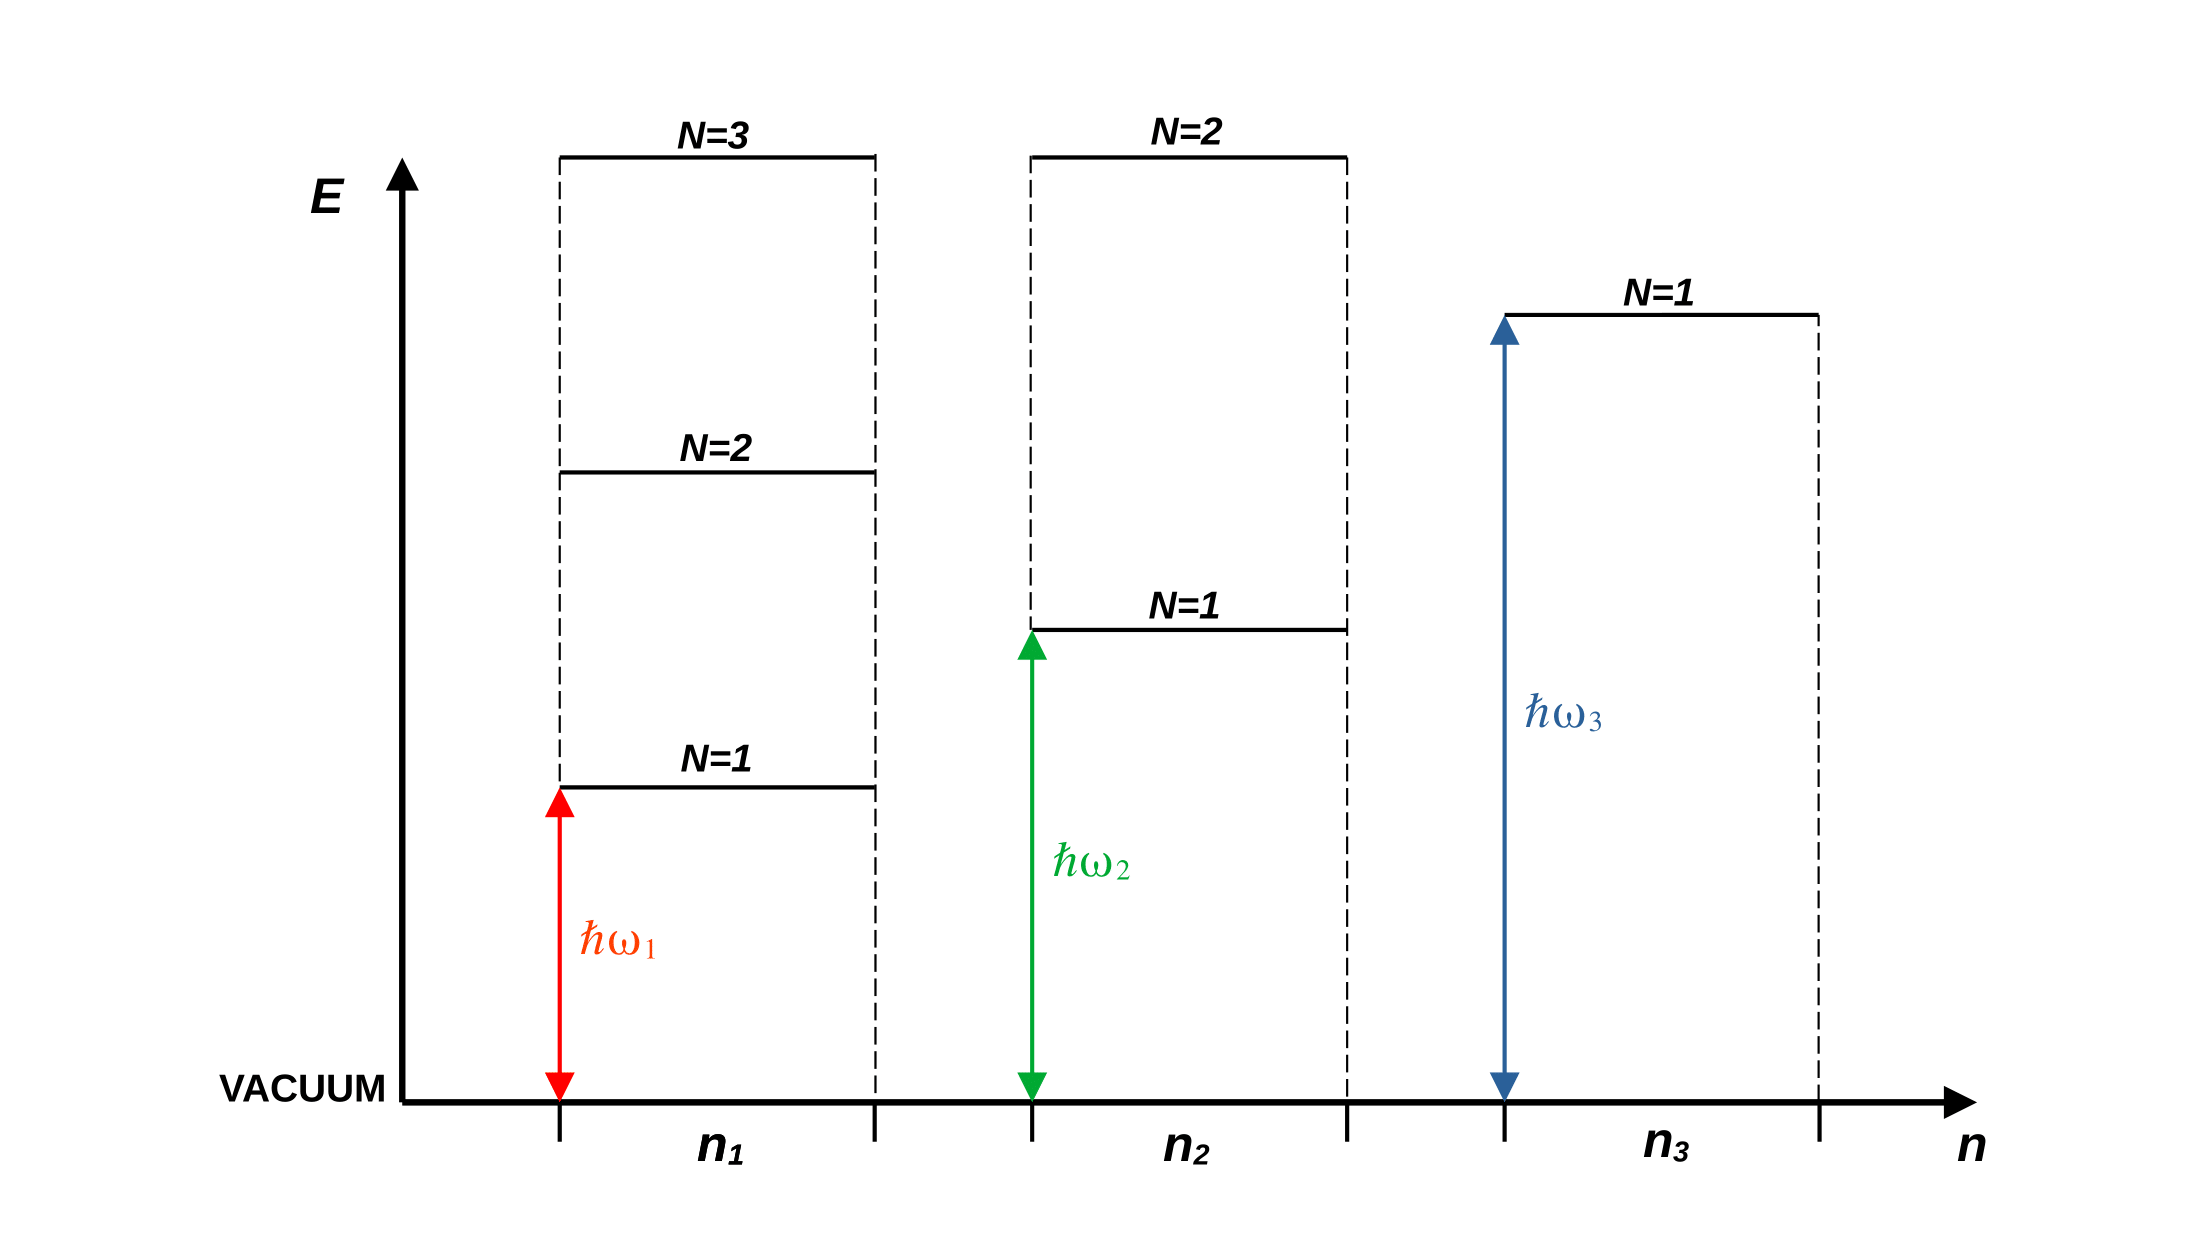
\includegraphics[width=0.8\linewidth]{images/Hilbert_space_QF.png}
\caption{Representation of the energy levels obtained from \ref{eq:Hmm}. Note that, in reality, every mode has a different value of point-zero energy.}
\label{fig:HspaceQF}
\end{figure}

\section{Electromagnetic fields in cavities}

\subsection{Cubic volume with periodic boundary conditions}
Consider a cubic volume $V=L_x L_y L_z$ with periodic boundary conditions, i.e. such that
\begin{align}
    \ux{x}{y}{z} &= \ux{x+L_x}{y}{z}, \\
    \ux{x}{y}{z} &= \ux{x}{y+L_y}{z}, \\
    \ux{x}{y}{z} &= \ux{x}{y}{z+L_z},
\end{align}
and take
\begin{align}
    \ur{}= u(\vec{r}) \vec{\epsilon} =  \frac{1}{\sqrt{V}}  \pw \vec{\epsilon}
\end{align}
as a possible solution for equation (\ref{eq:Hel}), where $\vec{\epsilon}$ is a tridimensional unitary vector. It is straightforward to prove that it is a solution 
\begin{align*}
    \left( \nabla^2  + \frac{\omega^2}{c^2} \right)\vec{\epsilon} \frac{1}{\sqrt{V}}  \pw = 
    \frac{\vec{\epsilon}}{\sqrt{V}} \left[ (i \vec{k})^2 + \frac{\omega^2}{c^2} \right] \pw = 
    \frac{\vec{\epsilon}}{\sqrt{V}} \left[ -k^2 + \frac{\omega^2}{c^2} \right] \pw = 0
\end{align*}
where in the last step the dispersion relation in vacuum ($\omega = k c$) is used.  \\
 
An important condition on $\vec{k}$ is found out from the periodic boundary conditions, indeed considering the one in the $z$-direction
\begin{gather*}
    \ux{x}{y}{z} = \ux{x}{y}{z+L_z} \quad \Longleftrightarrow \quad 
    \frac{\vec{\epsilon}}{\sqrt{V}} e^{i(x k_x + y k_y + z k_z)} = \frac{\vec{\epsilon}}{\sqrt{V}} e^{i(x k_x + y k_y + z k_z + L_z k_z)}
\end{gather*}
from which 
\begin{align}
    1 = e^{i L_z k_z} \quad \implies \quad k_z L_z = 2 \pi n_x \quad \Longleftrightarrow \quad k_z = \frac{2\pi}{L_z} n_z, \quad n_x \in \mathbb{Z}. 
    \label{eq:boundary}
\end{align}
One can repeat the same calculations for each direction. At the end, $\vec{k}$ must be:
\begin{equation}
    \vec{k} = \left( \frac{2 \pi}{L_x} n_x, \frac{2 \pi}{L_y} n_y, \frac{2 \pi}{L_z} n_z\right) \qquad \text{with} \qquad n_x, n_y, n_z \in \mathbb{Z}. 
\end{equation}
The numbers $n_x$, $n_y$ and $n_z$ are not independent, indeed the Coulomb gauge implies that
\begin{align*}
     \vec{\nabla} \cdot \vec{A} = \vec{\nabla} \cdot \ur{} = \vec{\nabla} \cdot \left(  \frac{\vec{\epsilon}}{\sqrt{V}} \pw \right) =
    \frac{\vec{\epsilon}}{\sqrt{V}} \cdot (i \vec{k}) \pw = 0 
\end{align*}
from which 
\begin{equation}
    \vec{\epsilon} \cdot \vec{k} = 0,
\end{equation}
where $\vec{\mathbf{\epsilon}}$ is the \textit{polarisation vector}. This relation shows that the electromagnetic field in vacuum is a transverse field. \\
The vector $\epsilon$ can be decomposed as the sum of two given basis vectors $\vec{\epsilon_{\lambda}}$ with $\lambda = 1, 2$ which lie in the plane perpendicular to $\vec{k}$, as shown in figure \ref{fig:Pol}. 
\begin{figure}[h!]
\centering
    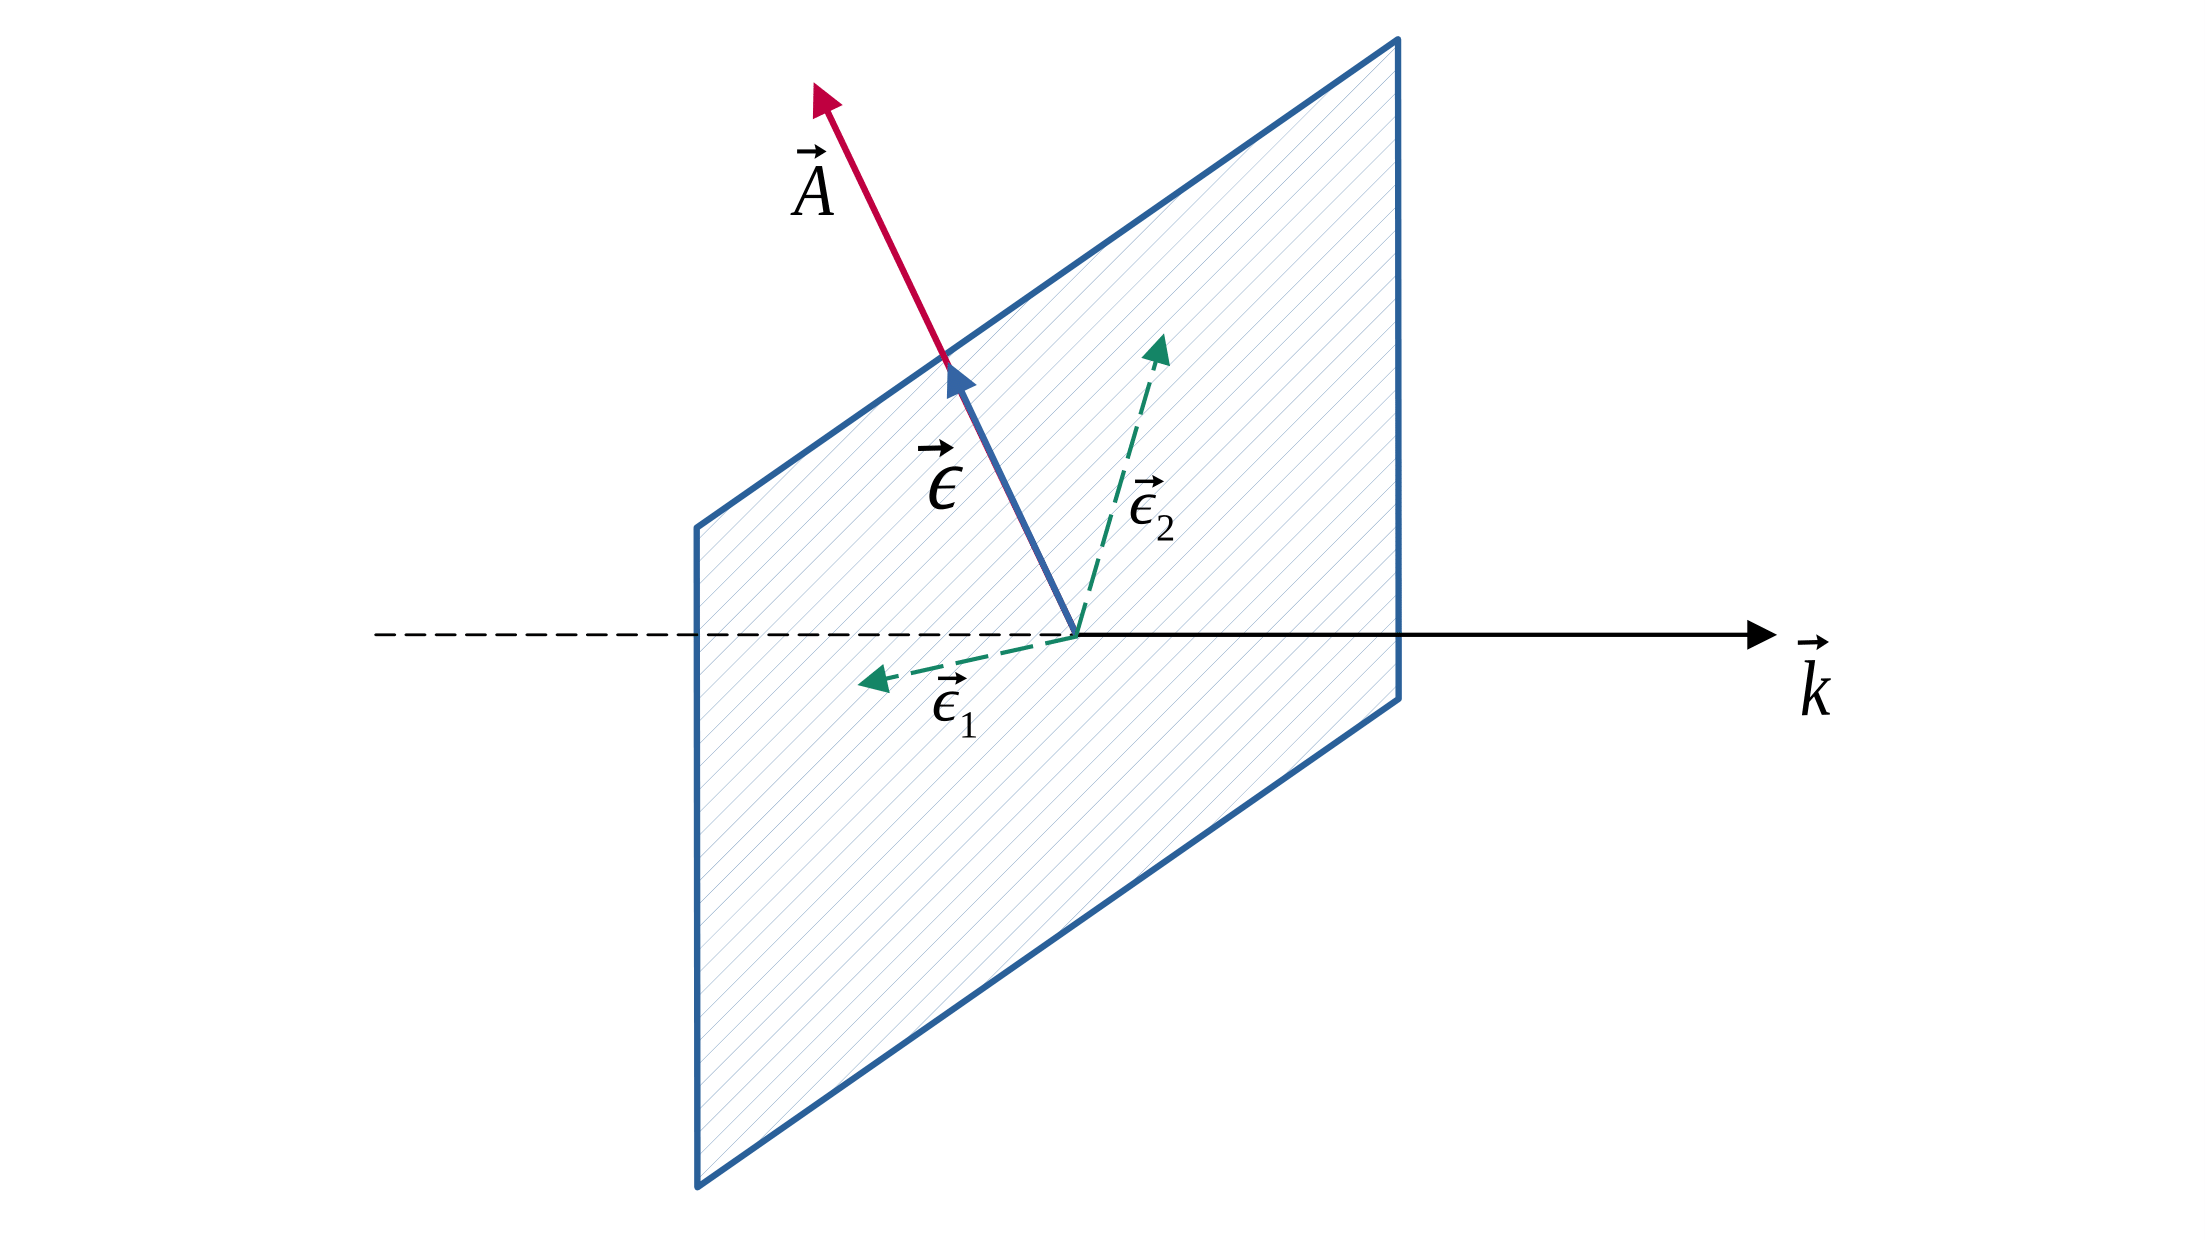
\includegraphics[width=0.78\linewidth]{images/Polarisation.png}
    \caption{Decomposition of the polarization vector $\vec{\epsilon}$ in the plane parallel to the propagation vector $\vec{k}$.}
    \label{fig:Pol}
\end{figure}

Therefore, the quantum field vectors and the Hamiltonian can be defined in terms of $\vec{k}$ and $\lambda$:
\begin{align}
     \A(\vec{r}, t) &= \sum\limits_{\vec{k}, \lambda} \sqrt{\frac{\hbar}{2 \varepsilon_{0} \omega_{k}}} \vec{\epsilon}_\lambda \left[ u_{\vec{k}, \lambda}^* \crt{\vec{k}, \lambda}   + u_{\vec{k}, \lambda} \dsr{\vec{k}, \lambda} \right], \label{eq:potvec}\\
     \hat{\vec{E}}(\vec{r}, t) &= -i \sum\limits_{\vec{k}, \lambda} \sqrt{\frac{\hbar \omega_k}{2 \varepsilon_0}} \vec{\epsilon}_{\lambda} \left[u_{\vec{k}, \lambda}^* \crt{\vec{k}, \lambda}  - u_{\vec{k}, \lambda} \dsr{\vec{k}, \lambda} \right], \label{eq:elfield}\\
     \hat{H} &= \sum\limits_{\vec{k}, \lambda} \hbar \omega_{\vec{k}} \, \crt{\vec{k}, \lambda} \dsr{\vec{k}, \lambda}. \label{eq:Hlight }
\end{align}
Notice that: 
\begin{itemize}
    \item the vacuum energy terms in the Hamiltonian is dropped with respect to the previous expressions (with a  finite number of dimensions that would not be a problem since the presence of a constant does not change the dynamics of the system; 
    \item the commutation relation between $\crt{\vec{k}, \lambda}$ and $\dsr{\vec{k}', \lambda'}$ becomes 
    \begin{equation}
        \left[\dsr{\vec{k}, \lambda}, \, \crt{\vec{k}', \lambda'}\right] = \mathbb{I} \delta_{\vec{k}, \vec{k'}} \delta_{\lambda, \lambda'}.
    \end{equation}
\end{itemize}

Finally, assuming $\vec{k} = (2 \pi/ L)\, \vec{n}$ and $\vec{k} \neq \vec{k'}$, the orthonormalization condition (\ref{eq:ortho}) is expressed as:
\begin{align*}
    \vec{\epsilon_{\lambda}} \cdot \vec{\epsilon_{\lambda'}} \int dV \frac{\pw}{\sqrt{V}} \frac{e^{-i\vec{k}'\cdot\vec{r}}}{\sqrt{V}} =
    &= \vec{\epsilon_{\lambda}} \cdot \vec{\epsilon_{\lambda'}}  \frac{1}{V} \int dV \exp{i(\vec{k}-\vec{k'} \cdot \vec{r})} =\\
    &= \vec{\epsilon_{\lambda}} \cdot \vec{\epsilon_{\lambda'}}  \frac{1}{V} \int dV \exp{i 2 \pi  \frac{(\vec{n} - \vec{n'}) \cdot \vec{r}}{L}  } = \\
    &= \vec{\epsilon_{\lambda}} \cdot \vec{\epsilon_{\lambda'}}  \frac{1}{V} \int dV  = \delta_{\lambda, \lambda'} = \delta_{\lambda, \lambda'} \delta_{k, k'}
\end{align*}
where $\delta_{k, k'}$ is introduced since the condition $\vec{k} \neq \vec{k'}$ is imposed at the beginning. \\

With this boundary conditions, one can evaluate the mean value and the variance of the electrical field. Consider a state with $n$ photons with the same mode identified by specific $\vec{k}$ and $\lambda$ and described by the Fock state
\begin{equation}
    \ket{\psi} = \ket{0} \otimes \ket{0} \otimes ... \otimes \ket{n_{\vec{k}, \lambda}} \otimes...\otimes \ket{0} \otimes \ket{0}
\end{equation}
and evaluate $\bra{\psi} \hat{\vec{E}} \ket{\psi} \equiv \langle \hat{\vec{E}} \rangle_\psi$. Remembering that 
\begin{align*}
    \bra{0} \crt{\vec{k}, \lambda} \ket{0} &= 0 \\
    \bra{0} \dsr{\vec{k}, \lambda} \ket{0} &= 0 
\end{align*}
and that 
\begin{align*}
    \bra{n_{\vec{k}, \lambda}} \crt{k, \lambda} \ket{n_{\vec{k}, \lambda}} &= \bra{n_{\vec{k}, \lambda}} \sqrt{n_{k, \lambda}+1} \ket{n_{\vec{k}, \lambda}+1} = 0, \\
    \bra{n_{\vec{k}, \lambda}} \dsr{k, \lambda} \ket{n_{\vec{k}, \lambda}} &= \bra{n_{\vec{k}, \lambda}} \sqrt{n_{k, \lambda}} \ket{n_{\vec{k}, \lambda}-1} = 0,
\end{align*}
one can conclude that $\langle \hat{\vec{E}} \rangle_\psi = 0$ $\forall \ket{\psi}$ and also on the vacuum, i.e. $\langle \hat{\vec{E}} \rangle_0 = 0$. \\
To evaluate the variance of the electrical field, notice that
\begin{equation*}
    \vec{E} \sim \crt{} + \dsr{} \qquad \text{while} \qquad \vec{E}^2 \sim \crt{}\crt{}, \, \dsr{}\dsr{}, \, \crt{}\dsr{}, \, \dsr{}\crt{}
\end{equation*}
and that the only combination of $\crt{}$ and $\dsr{}$ that given an average value which is different from $0$ (also for the vacuum state) is $\langle \dsr{}\crt{} \rangle_{\psi}$. Therefore, 
\begin{equation*}
    \langle \hat{\vec{E}}^2 \rangle_\psi = \sum\limits_{\vec{k}, \lambda} \frac{\hbar \omega_k}{2 \epsilon_0} \abs{\vec{\epsilon_{\lambda}}}^2 \abs{\ub{\vec{k}, \lambda}}^2 \langle \dsr{}\crt{} \rangle_{\psi} \neq 0 \qquad \implies \qquad \langle \hat{\vec{E}}^2 \rangle_0 \neq 0
\end{equation*}
from which 
\begin{equation}
    \Delta \hat{\vec{E}}_0^2 = \langle \hat{\vec{E}}^2 \rangle_0 -\langle \hat{\vec{E}} \rangle_0^2 = \langle \hat{\vec{E}}^2 \rangle_0 \neq 0. 
\end{equation}
This result is in contrast with the one obtained from classical considerations. 

\subsection{Fabry-Perot Cavity}

Consider a volume with dimensions such that $L_z \ll L_x, L_y $ which is delimited by two metallic mirrors located along the $z$-axis and placed perpendicular to it (figure \ref{fig:fp}).
The potential vector is taken with the following spatial dependence:
$${A(\vec{r})} = f_z (z) f_x (x) f_y (y),$$
where $f_x (x)$ and $f_y (y)$ are constant ($n_x =n_y = 0$). This means that the spatial dependence of the vector potential is only on $z$. \\
Since there are mirrors, the periodic boundary condition becomes
\begin{equation}
   \vec{u}(0) = \vec{u}(L_z) = 0, 
\end{equation}
if one is considering a cavity with the first mirror in $z = 0$ and the other in $z = L_z$. An expression for $\vec{u}(\vec{r})$ which satisfies it is 
\begin{equation}
    \ur{}= \vec{u}(z) = \vec{\epsilon}\sqrt{\frac{2}{V}} \sin(k_z z),
\end{equation}
(shown in figure \ref{fig:fp}) and hence the expression for the electric field is obtained from (\ref{eq:elfield}):
\begin{equation}
    \hat{\vec{E}}(\vec{r}, t) = -i \vec{\epsilon}_{\lambda} \sum\limits_{\vec{k}, \lambda} \sqrt{\frac{\hbar \omega_k}{ \varepsilon_0 V}}  \sin(k_z z) \left[ \crt{\vec{k}, \lambda}  - \dsr{\vec{k}, \lambda} \right]. 
    \label{eq:efFP}
\end{equation}

\begin{figure}[H]
\centering
    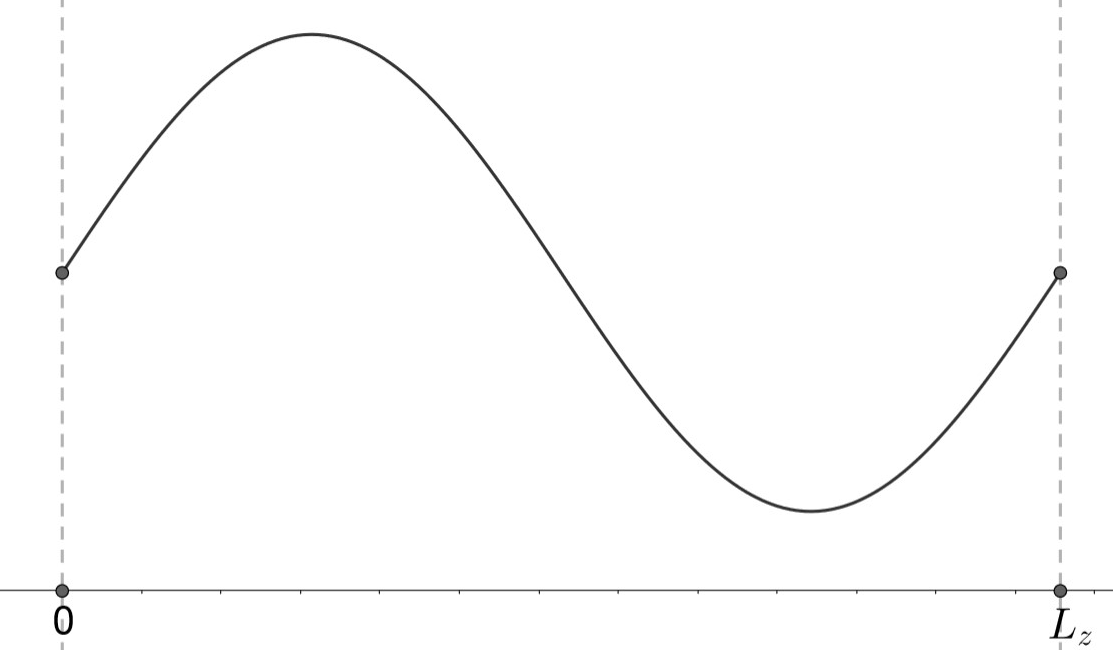
\includegraphics[width=0.65\linewidth]{images/Fabry_Perot.png}
    \caption{Function $\vec{u}(\vec{r})$ for a Fabry-Perot cavity with mirrors in $z = 0$ and $z = L_z$.}
    \label{fig:fp}
\end{figure}

Following the same steps of the previous section:
\begin{itemize}
    \item the boundary conditions (\ref{eq:boundary}) returns: 
    \begin{equation*}
        k_z L_z = \pi n \qquad \implies \qquad k_z =\frac{\pi}{L_z}n \quad \text{and} \quad \vec{u}(z) = \vec{\epsilon} \, \sqrt{\frac{2}{V}} \sin{\left( \frac{\pi}{L_z} n z \right)}
    \end{equation*}
    \item the normalisation condition (\ref{eq:norm_cond}) is verified:
    \begin{equation*}
        \int dV \, \urc{} \, \ur{} = L_x L_y \int dz \, f^{*}(z) f(z) = L_x L_y \int dz \, \frac{2}{V} \sin^2{\left(\frac{\pi}{L_z} n z \right)} = 1.
    \end{equation*}
\end{itemize}
In addition, one can compute the wave dispersion and the distance between two consecutive modes in the cavity:
\begin{equation*}
    \omega_n = c k_z^{(n)} = c \frac{\pi}{L_z}n \qquad \implies \qquad \Delta \omega_n = \frac{c \pi}{L_z}(n+1) - \frac{c \pi}{L_z}n = \frac{c \pi}{L_z}
\end{equation*}

\begin{tcolorbox} [breakable, enhanced]
Taking $L_z = 1$ cm, the separation of modes is about $\Delta \omega_n \simeq  100 $ GHz (microwave-infrared range). \\
The possibility of having a large separation between modes allows to do \textit{single-mode cavity physics}:
\begin{equation*}
    H = \sum\limits_n \hbar \omega_n \crt{n}\dsr{n} \qquad  \longrightarrow \qquad  \hbar\omega \crt{} \dsr{}. 
\end{equation*}
This is useful when an atom inside the cavity emits a single photon at frequency $\omega$, which can be obtained with a proper realisation of the cavity (the modes are \textit{off-resonant} with respect to an atomic transition). 
\end{tcolorbox}

As in the previous subsection, the average value and the variance (evaluated on the vacuum state) of the electric field can be computed. In particular, 
\begin{align*}
    \langle \hat{\vec{E}} \rangle_0 &= 0 \\ 
   \langle \hat{\vec{E}}^2 \rangle_0 &= \frac{\hbar \omega}{2 \epsilon_0} \frac{2}{V} \sin^2\left(\frac{\pi}{L}n z\right) \sim \frac{1}{V}
\end{align*}
and in the centre of the cavity (for $z = L/2$)
$$\langle \hat{\vec{E}}^2 \rangle_0 = \frac{\hbar \omega}{2 \epsilon_0} \frac{1}{V} \neq 0.$$

\section{Coherent states}

It is possible to obtain the states on which the average value of the electric field operator is not null: they are called \textit{coherent states}, usually indicated with $\ket{\alpha_c}$. Using the results of the previous sections, one deduces that they have to satisfy the relations: 
\begin{equation}
    \begin{cases}
        \dsr{} \ket{\alpha_c} = \alpha_c(t) \ket{\alpha_c}, \\
        \bra{\alpha_c} \crt{} = \alpha_c^*(t) \bra{\alpha_c}.
    \end{cases}
\end{equation}
Then, working in the single mode approximation to simplify the steps, one can derive the expression for the average value of the electric field in a Fabry-Perot cavity starting form the expression for $\hat{\vec{E}}$ 
\begin{align}
 \hat{\Vec{E}}(z,t) = - i \ \Vec{\epsilon} \sqrt{\frac{\hbar \omega}{V \varepsilon_0}} \sin\left(k_z z\right) \left[\crt{}(t) - \dsr{}(t)\right]
\end{align}
and evaluating 
\begin{align*}
    \bra{ \alpha_c} \hat{\Vec{E}} \ket{\alpha_c} & =  - i \Vec{\epsilon} \sqrt{\frac{\hbar \omega}{V \varepsilon_0}} \sin(k_z z) \left(\bra{\alpha_c} \crt{} \ket{\alpha_c} - \bra{\alpha_c} \dsr{} \ket{ \alpha_c} \right) \\
    & = - i \Vec{\epsilon} \sqrt{\frac{\hbar \omega}{V \varepsilon_0}} \sin(k_z z) \left(\alpha_c^*(t) - \alpha_c(t)\right) \\
    & = -i  \Vec{\epsilon} \sqrt{\frac{\hbar \omega}{V \varepsilon_0}} \sin(k_z z) \alpha_c(0) \left(e^{\text{i} \omega t} - e^{- \text{i} \omega t}\right) \\
    & = 2 \Vec{\epsilon} \ \sqrt{\frac{\hbar \omega}{V \varepsilon_0}} \sin(k_z z) \sin(\omega t) \alpha_0. 
\end{align*}
In addition to this, one can evaluate the variance of this electric field operator over the coherent states, which leads to:
\begin{align}
    \Delta \hat{\vec{E}}_0^2 & = \left< \alpha_c \right| \hat{\Vec{E}} \cdot \hat{\Vec{E}}\left| \alpha_c \right> - \left( \left< \alpha_c \right| \Vec{E} \left| \alpha_c \right> \right)^2 = \frac{\hbar \omega}{V \varepsilon_0} \sin^2(k_z z), 
\end{align}
since one can prove that
\begin{align*}
    \left< \alpha_c \right| \hat{\Vec{E}} \cdot \hat{\Vec{E}}\left| \alpha_c \right> = \left( \left< \alpha_c \right| \Vec{E} \left| \alpha_c \right> \right)^2 + \frac{\hbar \omega}{V \varepsilon_0} \sin^2(k_z z). 
\end{align*}
In order to evaluate the impact of these fluctuations, one can consider:
\begin{equation}
    \frac{\Delta \hat{\vec{E}}_0^2}{\left| \left< \alpha_c \right| \Vec{E} \left| \alpha_c \right>\right|^2} = \frac{1}{\alpha_c^* (t) - \alpha_c(t)} \sim \frac{1}{\left| \alpha_c(t) \right|} \sim \frac{1}{\left| \alpha_c(0) \right|} 
\end{equation}
This quantity goes to 0 when $\alpha_c(0) \gg 1$, i.e. in a classical situation, in which there is a large number of photons in a coherent state and the addition or the removal of one of them does not have any impact. Indeed $\left| \alpha_c(t) \right|$ corresponds to the expectation value of the number operator $\hat{N}$: 
\begin{equation}
    \left< \alpha_c \right| \hat{N} \left| \alpha_c \right> = \left< \alpha_c \right| \crt{} \, \dsr{} \left| \alpha_c \right> = \left< \alpha_c \right| \alpha^*_c(t) \, \alpha_c(t) \left| \alpha_c \right> = \left| \alpha_c(t) \right|^2.
\end{equation}

\subsection{Glauber's coherent states and occupation probabilities}

\begin{figure}[t!]
\centering
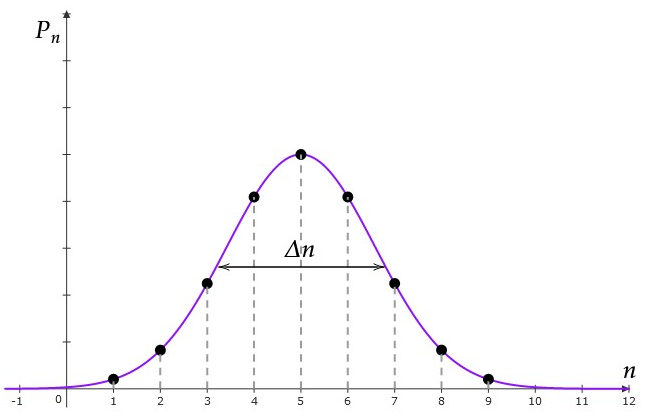
\includegraphics[width=0.7\linewidth]{images/Poisson.png}
\caption{Probability of finding or measuring $n$ photons in a generic coherent state $\ket{\alpha_c}$; for large values of $| \alpha_c|$ it resembles the normal distribution.}
\label{fig:Poisson}
\end{figure}

A generic coherent state $\ket{\alpha_c}$ can be expanded in terms of Fock states
\begin{equation}
    \left| \alpha_c \right> \equiv e^{-\left| \alpha_c \right|^2 / 2} \sum_{n=0}^{\infty} \frac{\alpha_c^n}{\sqrt{n!}} \left| n \right>
    \label{eq:cohstate}
\end{equation}
and it is called \textit{Glauber's coherent state}. \\
From this expression, it is possible to evaluate the probability of finding or measuring $n$ photons in a generic coherent state $\ket{\alpha_c}$: 
\begin{equation*}
    P_n \equiv \left| \bra{n}\ket{\alpha_c}\right|^2 = \left| e^{-\left| \alpha_c \right|^2/2} \frac{\alpha_c^n}{\sqrt{n!}}  \right|^2 =  e^{-\left| \alpha_c \right|^2} \, \frac{\alpha_c^{2n}}{n!},
\end{equation*}
which is a Poisson's distribution with variance $\Delta n = | \alpha_c|$, as shown in figure \ref{fig:Poisson}. 

\subsection{Generation of a coherent state}
A coherent state can be generated starting from the Hamiltonian
\begin{equation*}
    \hat{H} = F \cos (\omega t) \left(\hat{a}^{\dagger} + \hat{a}\right), 
\end{equation*}
where $F$ is the driving force, starting from the vacuum state $\ket{0}$.


\chapter{Hydrogen-like atoms}
% -----------------------------------------------------------
%
%  CHAPTER 4  of Quantum information with atoms and photons
%
%  written by many authors Jan 2023
% -----------------------------------------------------------



The structure of the energy levels of a given atomic system can be different according to the resolution adopted to resolve it and which type of interactions have been considered. In particular, three structures are present: 

\begin{table}[h!]
\centering
\begin{tabular}{c|c|c|c}
\toprule
 $~$ \textbf{Structure} $~$  & $~$ \textbf{Energy} $~$ & $~$ \textbf{Frequency} $~$  & $~$  \textbf{Source} $~$ \\
\hline
\textit{Gross} & 1-10 eV & \makecell{$>$ 200 THz \\ (visible light)} &\makecell{nucleus-electron interaction \\ electron-electron interaction \\ and kinetic energy} \\ %\hline
\textit{Fine} & 10$^{-3}$-$10^{-2}$ eV & \makecell{$\sim$  1 THz \\ (far infra-red)} & \makecell{spin-orbit interaction \\ (relativistic effect)}\\ %\hline
\textit{Hyperfine} & 10$^{-6}$-$10^{-5}$ eV & \makecell{$\sim$ 1 GHz \\ (micro-wave)} & \makecell{magnetic dipole coupling \\ (nucleus-electron magnetic \\ interaction)} \\
\bottomrule
\end{tabular}
\caption{Atomic energy structures whit typical energies, frequencies and source of the spectra. }
\label{tab:en_lev}
\end{table}

In the following, only the first two structures are considered.

\section{From the Hydrogen atom to the Alkali}

An \textit{hydrogenoid atomic system} (which includes hydrogen atoms and Alkali atoms) is made of two elements:
\begin{itemize}
    \item a heavy attractor (the nucleus and the electrons of the inner shell) characterized by a mass $m_H$ and a momentum $\vec{p}_H$; 
    \item a light attractor (the outer electron) characterized by a mass $m_e$ and a momentum $\vec{p}_e$. 
\end{itemize}
The Hamiltonian of the system is 
\begin{align}
    H = \frac{\abs{\vec{p}_H}^2}{2 m_H} + \frac{\abs{\vec{p}_e}^2}{2 m_e} + V(\abs{\vec{r}_H - \Vec{r_e}}), 
    \label{eq:Hatoms1}
\end{align}
Where the first two terms are the kinetic energies of the heavy and light attractors, while the potential depends only on the modulus of the distance between them (radial potential).
Moreover, for $\vec{r}_H$, $\vec{r}_e$, $\vec{p}_H$ and $\vec{p}_e$
\begin{align}
    [({r}_H)_j,({p}_H)_k] &= i \hbar \delta_{jk}, \label{eq:comm1} \\
    [({r}_e)_j,({p}_e)_k] &= i \hbar \delta_{jk}, \label{eq:comm2} \\
    [({r}_e)_j,({p}_H)_k] &= [(\vec{r}_H)_j,(\vec{p}_e)_k] = 0. \label{eq:comm3}
\end{align}
The Hamiltonian $H$ in (\ref{eq:Hatoms1}) can be rewritten introducing the following change of coordinates:
\begin{align*}
    \text{Centre-of-mass coordinate} \qquad \vec{R} &\equiv \dfrac{\vec{r}_H m_H + \vec{r}_e m_e }{m_H + m_e} \\
    \text{Relative coordinate} \qquad \vec{r} &\equiv \vec{r}_e - \vec{r}_H  \\
    \text{Centre-of-mass momentum} \qquad \vec{P} &\equiv \vec{p}_H + \vec{p}_e   \\
    \text{Relative momentum} \qquad \vec{p} &\equiv \dfrac{\dfrac{\vec{p}_e}{m_e} - \dfrac{\vec{p}_H}{m_H}}{\dfrac{1}{m_e} + \dfrac{1}{m_H}} 
\end{align*}
and from relations (\ref{eq:comm1}), (\ref{eq:comm2}) and (\ref{eq:comm3}), one can obtain
\begin{align}
    [R_j,P_k] = i \hbar \delta_{jk}. 
\end{align}
Therefore, the Hamiltonian in (\ref{eq:Hatoms1}) becomes
\begin{align}
    H = \frac{|{\vec{P}}|^2}{2 m_+} + \frac{|{\vec{p}}|^2}{2 m} + V(\abs{\underbrace{\vec{r}_H - \Vec{r_e}}_{\vec{r}}}), 
    \label{eq:Hatoms2}
\end{align}
where
\begin{align*}
    m_+ \equiv m_H + m_e \simeq m_H \qquad \text{and} \qquad \frac{1}{m} \equiv \left( \frac{1}{m_H} + \frac{1}{m_e}  \right) \simeq \frac{1}{m_e}
\end{align*}
are the total and reduced mass, respectively. \\

In order to rearrange again (\ref{eq:Hatoms2}), it is necessary to introduce the \textit{orbital angular momentum operator}. 

\subsection{Orbital angular momentum operator}

The angular momentum is a pseudo-vector defined as
\begin{equation}
    \Vec{L} = \Vec{r} \, \cross \, \Vec{p} = \begin{pmatrix}
        r_yp_z - r_zp_y \\
        r_zp_x - r_xp_z \\
        r_xp_y - r_yp_x \\
    \end{pmatrix},
    \label{eq:Ldef}
\end{equation}
where the general $i$-th component is given by 
\begin{align}
    L_i = -i\hbar \hat{r}\cross \nabla = -i \hbar \left(x_j \frac{\partial}{\partial x_k} - x_k \frac{\partial}{\partial x_j}\right) \qquad i,j,k = x,y,z.
    \label{eq:Li}
\end{align}
The operator $L$ satisfies the commutation rules
\begin{equation}
    [L_i,L_j]=i \hbar \epsilon_{ijk} L_k. 
    \label{eq:commu1}
\end{equation}

\begin{tcolorbox} [breakable, enhanced]
\textbf{Explicit evaluation of $[L_x,L_y]$} 
\begin{align*}
    [L_x,L_y] &= -\hbar^2\bigl((y\partial_z - z \partial_y)(z \partial_x - x \partial_z) - (z \partial_x - x \partial_z)(y \partial_z - z \partial_y)\bigl) = \\
     &= -\hbar^2\bigl[\bigl(y\partial_z(z \partial_x) - y \partial_z (x \partial_z) - 
    z \partial_y (z \partial_x) + z \partial_y (x \partial_z) \bigl) + \\
    & \qquad -\bigl(z \partial_x (y \partial_z) - z \partial_x (z \partial_y) - x \partial_z (y \partial_z ) + x \partial_z (z \partial_y)\bigl) \bigl] =  \\
    &= -\hbar^2\bigl[\bigl(y \partial_x (\partial_z z) + yz \partial_z \partial_x - yx \partial^2_z - z^2 \partial_y \partial_x + zx \partial_y \partial_z \bigl) = \\
    & \qquad - \bigl(zy \partial_x \partial_z - z^2 \partial_x \partial_y - xy \partial_z^2 + x \partial_y (\partial_z z) + xz \partial_x \partial_y \bigl) \bigl] = \\
    &= \hbar^2 ( x \partial_y - y \partial_x ) = \hbar^2 \frac{L_z}{-i\hbar} =  i\hbar L_z
\end{align*}
\end{tcolorbox}

Relation (\ref{eq:commu1}) shows that $\vec{L}$:
\begin{itemize}
    \item has the mathematical structure of a Lie algebra and the $\epsilon_{ijk}$ are its structure constants;
    \item plays a central role in quantum problems involving rotational symmetry and its most general and fundamental definition is the \textit{generator of rotations}
    \begin{align*}
        R(\theta,\varphi,\chi) = \exp{\frac{i}{\hbar}L_z \chi} \exp{\frac{i}{\hbar}L_x \theta} \exp{\frac{i}{\hbar}L_z \varphi},
    \end{align*}
    where $\theta$, $\varphi$ and $\chi$ are the conventional Euler angles. 
\end{itemize}

The other essential commutator rule is
\begin{equation}
    [L_i,L^2] = 0, \qquad \forall i = x,y,z.
    \label{eq:commu2}
\end{equation}

\begin{tcolorbox}[breakable, enhanced]
\textbf{Explicit evaluation of $[L_z,L^2]$} 
    \begin{align*}
        [L_z,L^2] &= [L_z,L_x^2] + [L_z,L_y^2] = \\
        &= [L_z,L_x]L_x + L_x[L_z,L_x] + [L_z,L_y]L_y + L_y[L_z,L_y] = \\
        &= i\hbar (L_y L_x + L_x L_y - L_xL_y - L_y L_x) = 0
    \end{align*}
\end{tcolorbox}

If one fixes the $z$-axis as the reference direction (defining suitable spherical coordinates), relation (\ref{eq:commu2}) ensures that there is a common basis of eigenstates for $L_z$ and $L^2$. These eigenstates $\psi$ are functions of two labels $l$ and $m$ such that
\begin{align}
    L_z \psi(l,m) = \hbar m \, \psi(l,m) \qquad \text{and} \qquad L^2 \psi(l,m) = f(l) \, \psi(l,m),
    \label{eq:eigenvaleq}
\end{align}
where $f(l)$ is a function of $l$.

Note that $\psi(l,m)$ could have some degeneracy if only $l$ and $m$ are specified. However, this will not occur for the orbital angular momentum as we will show that its eigenfunctions are spherical harmonics that form a full base of $L^2$.

\subsubsection{Raising and lowering operators}

At this point, it is convenient to define the \textit{raising} and \textit{lowering operators}
\begin{equation}
    L_\pm = L_x \pm i L_y
    \label{eq:lpm}
\end{equation}
with commutation rules
\begin{equation}
    [L_+,L_-] = 2 \hbar \, L_z \qquad \text{and} \qquad [L_z,L_\pm] = \pm \hbar \, L_\pm.
\end{equation}

\begin{tcolorbox}[breakable, enhanced]
\textbf{Explicit evaluation of $[L_+,L_-]$} 
    \begin{align*}
    [L_+,L_-] & = L_+ L_- - L_- L_+ = (L_x + iL_y)(L_x - iL_y) - (L_x - iL_y)(L_x + iL_y) = \\
    & = (L_x^2 -i L_xL_y +i L_yL_x + L_y^2) - (L_x^2 + iL_xL_y - iL_yL_x + L_y^2) = \\
    & = -2i [L_x,L_y] = 2\hbar L_z
\end{align*} 
\end{tcolorbox}

\begin{tcolorbox}[breakable, enhanced]
\textbf{Explicit evaluation of $[L_z,L_\pm]$} 
    \begin{align*}
    [L_z,L_\pm] &= L_z(L_x \pm iL_y)-(L_x \pm iL_y)L_z = \\
    & = L_zL_x\pm iL_zL_y-L_xL_z\mp iL_yL_z = \\
    & = i\hbar L_y \pm \hbar L_x = \pm \hbar L_\pm
    \end{align*}
\end{tcolorbox}

From (\ref{eq:lpm}), one can notice that $L_\pm$ are not Hermitian since $(L_\pm)^\dagger = L_\mp$. In addition, it is possible to write 
\begin{align}
    L^2 = L_x^2 + L_y^2 + L_z^2 = L_- L_+ + L_z^2 + \hbar L_z = L_+ L_- + L_z^2 - \hbar L_z  
    \label{eq:L2}
\end{align}
and to conclude that 
\begin{align}
    [L^2,L_\pm] = 0. 
\end{align}

\begin{tcolorbox} [breakable, enhanced]
\textbf{Proof of (\ref{eq:L2})} \\
The terms $L_- L_+$ and $L_+ L_-$ are evaluated explicitly:
\begin{align*}
    L_- L_+ &= (L_x - i L_-)(L_x + i L_-) = L_x^2 + i L_x L_y - i L_y L_x + L_y^2 = \\
    &= L_x^2 + L_y^2 +i [L_x,L_y] = L_x^2 + L_y^2 - \hbar L_z, \\ 
    L_+ L_- &= (L_x + i L_-)(L_x - i L_-) = L_x^2 - i L_x L_y + i L_y L_x + L_y^2 = \\
    & = L_x^2 + L_y^2 -i [L_x,L_y] = L_x^2 + L_y^2 + \hbar L_z.
\end{align*}
From these result, relation (\ref{eq:L2}) follows immediately. 
\end{tcolorbox}

\begin{tcolorbox} [breakable, enhanced]
\textbf{Explicit evaluation of $[L^2,L_\pm]$} 
\begin{align*}
    [L^2,L_\pm] &= [L_+L_-+L_z^2-\hbar L_z,L_\pm] = \\
    & = [L_+L_-,L_\pm] + [L_z^2,L_\pm] - \hbar[L_z,L_\pm] = \\
    &= [L_+,L_\pm]L_- + L_+[L_-,L_\pm] + [L_z,L_\pm]L_z + L_z [L_z,L_\pm] - \hbar [L_z,L_\pm].
\end{align*}
For clarity, it is now convenient to compute separately the cases $L_+$ and $L_-$:
\begin{align*}
    [L^2,L_+] &=  [L_+,L_+]L_- + L_+[L_-,L_+] + [L_z,L_+]L_z + L_z [L_z,L_+] - \hbar [L_z,L_+] = \\
    &=  -2\hbar L_+L_z + \hbar L_+L_z + \hbar L_zL_+ - \hbar^2 L_+ = \\
    &= \hbar(L_zL_+-L_+L_z)-\hbar^2L_+ = \\
    &= \hbar[L_z,L_+] - \hbar^2 L_+ = \hbar^2 (L_+ - L_+) = 0, \\
    [L^2,L_-] &= [L_+,L_-]L_- + L_+[L_-,L_-] + [L_z,L_-]L_z + L_z [L_z,L_-] - \hbar [L_z,L_-] = \\
    & = 2\hbar L_zL_- - \hbar L_-L_z - \hbar L_zL_- + \hbar^2 L_- = \\
    & = -\hbar(L_zL_--L_-L_z)+\hbar^2L_+ = \\
    & = -\hbar[L_z,L_-] + \hbar^2 L_- = -\hbar^2 (L_- - L_-) = 0.
\end{align*}
\end{tcolorbox}
It is now possible to study the effect of $L_z$ and $L^2$ on a state $\psi(l,m)$ on which acts $L_\pm$: 
\begin{align}
    L^2 \left( L_\pm \psi (l,m) \right) &= L_\pm \left( L^2 \psi (l,m) \right) = f(l) \left( L_\pm \psi (l,m) \right) \label{eq:prop1} \\
    L_z \left( L_\pm \psi (l,m) \right) &= L_\pm L_z \psi (l,m) + [L_z, L_\pm] \, \psi (l,m) = \nonumber \\
    &= \hbar m \left( L_\pm \psi (l,m) \right) \pm \hbar \left( L_\pm \psi (l,m) \right) = \nonumber \\
    &= \hbar (m \pm 1) \left( L_\pm \psi (l,m) \right) \label{eq:prop2}
\end{align}
From the result in (\ref{eq:prop1}), one can conclude that $L_\pm \psi (l,m)$ is an eigenstate of $L^2$ and also that it does not impact on his eigenvalues. While from (\ref{eq:prop2}) it is possible to identify two cases: 
\begin{itemize}
    \item \textbf{Case 1} \\
    Equation (\ref{eq:prop2}) is trivially satisfied if $L_\pm \psi (l,m) = 0$.  This case suggests that there must exist two values of $m$, $m_\text{max}$ and $m_\text{min}$, such that
\begin{align}
    L_+\psi(l,m_\text{max}) = 0 \qquad \text{and} \qquad L_- \psi(l,m_\text{min}) = 0. 
\end{align}
From this
\begin{align*}
        L^2 \psi(l,m_\text{max}) &= (L_- L_+ + L_z^2 + \hbar L_z) \, \psi(l,m_\text{max}) = \\ 
        &= L_-(L_+\psi(l,m_\text{max})) + L_z^2\psi(l,m_\text{max}) +\hbar L_z \psi(l,m_\text{max}) = \\ 
        &= \hbar^2 m_\text{max} (m_\text{max} + 1) \, \psi(l,m_\text{max}) = f(l) \, \psi(l,m_\text{max}), \\
        L^2 \psi(l,m_\text{min}) &= (L_+L_- + L_z^2 - \hbar L_z) \, \psi(l,m_\text{min}) = \\
        &= L_+(L_-\psi(l,m_\text{min})) + L_z^2\psi(l,m_\text{min}) -\hbar L_z \psi(l,m_\text{min}) = \\ 
        &= \hbar^2 m_\text{min} (m_\text{min} - 1) \, \psi(l,m_\text{min}) = f(l) \, \psi(l,m_\text{min}).
\end{align*}
Notice that the results presents the same function $f(l)$ because the function $\psi$ has the same $l$ value in both the calculations. Therefore, 
\begin{equation}
        f(l) = \hbar^2 m_\text{max} (m_\text{max} + 1) = \hbar^2 m_\text{min} (m_\text{min} - 1), \qquad m_\text{max} - m_\text{min} \in \mathbb{N}
    \label{eq:sistmaxmin}
\end{equation}

\begin{tcolorbox}
\textbf{Solution of (\ref{eq:sistmaxmin})} \\
The general solution can be found by introducing a number $a \in \mathbb{N}$ in such a way that
    \begin{align*}
        \begin{cases}
        m_\text{min} = m_\text{max} - a \\
        m_\text{max} (m_\text{max} + 1) = m_\text{min} (m_\text{min} - 1) 
    \end{cases}
    \end{align*}
    By substituting the first equation in the second one
    \begin{align*}
    & m_\text{max}^2 + m_\text{max} - (m_\text{max} - a)^2 + (m_\text{max} - a) = \\
    & = m_\text{max}^2 + m_\text{max} - m_\text{max}^2 -a^2 +2 m_\text{max}a + m_\text{max} - a = 0 
    \end{align*}
    and hence 
    \begin{align*}
         2m_\text {max}(a+1) = a(a+1) \qquad & \implies \qquad  m_\text{max} = \frac{a}{2}, \\
         & \implies \qquad m_\text{min} = -\frac{a}{2}.
    \end{align*}
\end{tcolorbox}
This implies that $m_\text{max}$ and $m_\text{min}$ can only be integer or half integer: $m_\text{max}$, $m_\text{min} \in \dfrac{\mathbb{N}}{2}$.

From now on, consider 
\begin{align*}
    l \equiv m_\text{max} \qquad \implies \qquad & f(l) = \hbar^2 l(l+1) \qquad \text{and} \qquad l \in \frac{\mathbb{N}}{2}
\end{align*}
    
    \item \textbf{Case 2} \\
    Since the eigenvalue of equation (\ref{eq:prop2}) is $\hbar(m \pm 1)$, $L_\pm \psi (l,m)$ must be proportional to a an eigenfunction $\psi'(m,l+1)$ associated to that eigenvalue. Therefore, using the bra-ket notation, one can write
    \begin{align}
        & L_+ \ket{l,m} = \alpha \, \ket{l,m + 1} \qquad \text{with} \qquad \alpha \in \mathbb{C} \label{eq:L+a} \\
        & L_- \ket{l,m+1} = \beta \, \ket{l,m} \qquad \text{with} \qquad \beta \in \mathbb{C} \label{eq:L-a}
    \end{align}
    and notice that
    \begin{align*}
        \beta = \bra{l,m} L_- \ket{l,m+1} = \left( \bra{l,m+1} L_+ \ket{l,m} \right)^* = \alpha^*. 
    \end{align*}
    Therefore, using this result and the expression (\ref{eq:L2}) for $L^2$, 
    \begin{align*}
        L_- L_+ \ket{l,m} &= \abs{\alpha}^2 \ket{l,m} = (L^2 - L_z^2 - \hbar L_z) \ket{l,m} = \\
        & = \hbar^2 [l(l+1) - m^2 - m)] \ket{l,m} \\
        & = \hbar^2 [l(l+1) - m(m+1)] \ket{l,m} \\
        L_+ L_- \ket{l,m+1} &= \abs{\beta}^2 \ket{l,m+1} = (L^2 - L_z^2 + \hbar L_z) \ket{l,m+1} = \\
        & = \hbar^2 [l(l+1) - m^2 - m)] \ket{l,m+1} \\
        & = \hbar^2 [l(l+1) -m(m+1)] \ket{l,m+1} 
    \end{align*}
    If $\alpha$ and $\beta$ are real, one can conclude that 
    \begin{align}
        \alpha = \beta = \hbar \sqrt{l(l+1) - m(m+1)}
        \label{eq:alphabeta}
    \end{align}
    Hence, unifying (\ref{eq:L+a}), (\ref{eq:L-a}) and (\ref{eq:alphabeta})
    \begin{align}
        L_+ \ket{l,m} &=  \hbar \sqrt{l(l+1) - m(m+1)} \ket{l,m + 1} \label{eq:L+action}\\
        L_- \ket{l,m} &=  \hbar \sqrt{l(l+1) - m(m-1)} \ket{l,m -1} \label{eq:L-action}
    \end{align}
    The action of $L_+$ and $L_-$ on a state $\ket{l,m}$ is shown in figure \ref{fig:lowrai}. 
    \begin{figure}[h!]
\centering
    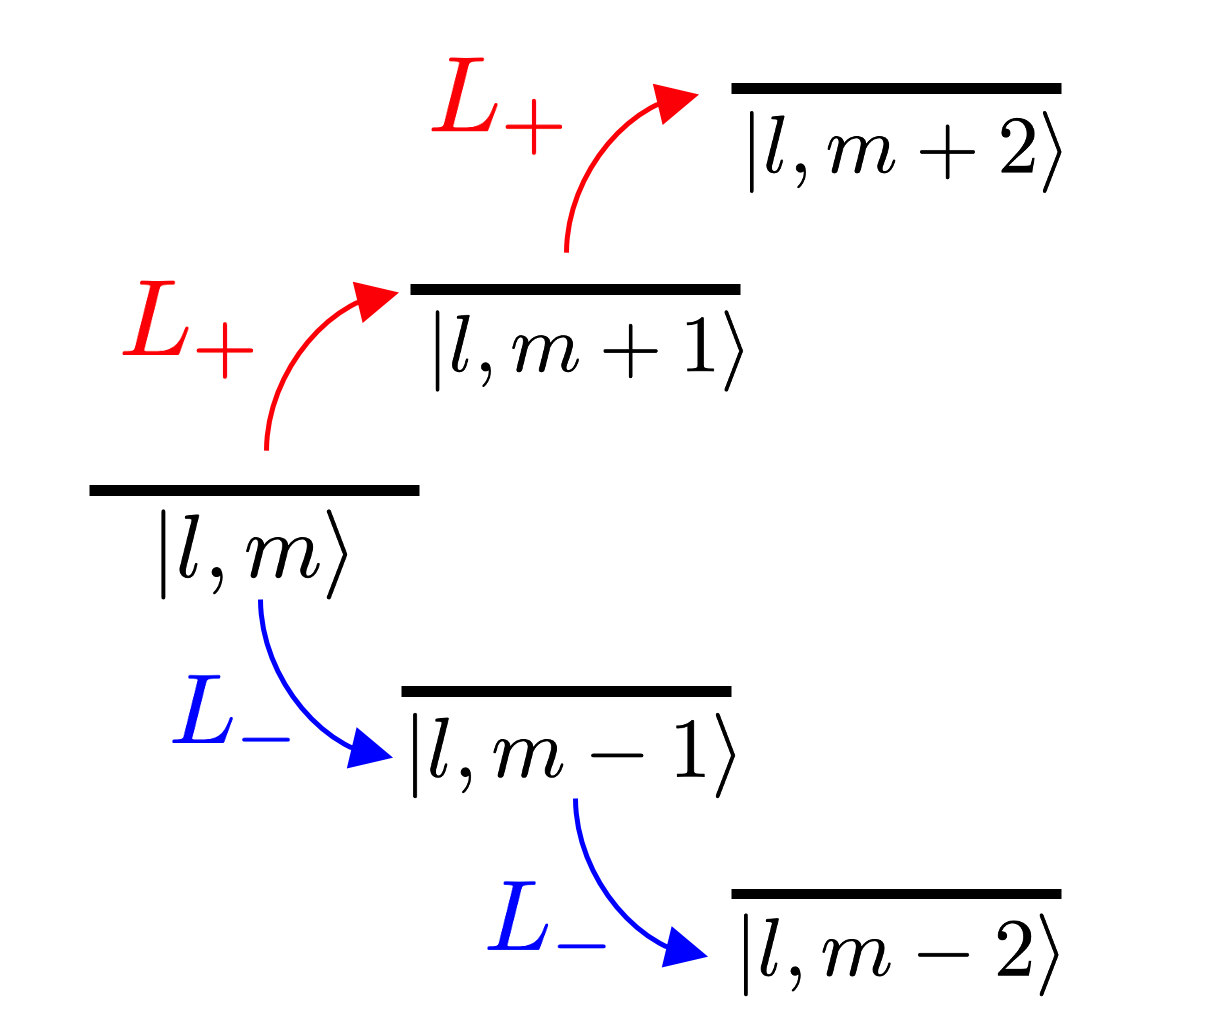
\includegraphics[width=0.35\linewidth]{images/Lowering_Raising_operators.png}
    \caption{Action of the lowering and raising operators $L_-$ and $L_+$; they lower and raise by 1 the quantum number $m$ of the state on which act.}
    \label{fig:lowrai}
\end{figure}
\end{itemize}
Summarizing the results 
\begin{align}
    & L^2 \psi(l,m) = \hbar^2 l(l+1) \psi(l,m) \qquad \text{with} \qquad l \in \frac{\mathbb{N}}{2} \\
    & L_z \psi(l,m) = \hbar m \psi(l,m), \qquad \text{with} \qquad m \in \, \{-l, \, ..., \, +l \}
\end{align}

It is important to notice that these rules follow only from the Lie algebra of the angular momentum operators; by concerning the orbital angular momentum defined in (\ref{eq:Ldef}), it is possible to deduce further restrictions on $l$. Indeed, introducing
\begin{align*}
    r_1 = \frac{r_x+p_y}{\sqrt{2}}, \qquad p_1 = \frac{r_x-p_y}{\sqrt{2}}, \qquad r_2 = \frac{p_x-r_y}{\sqrt{2}} \qquad \text{and} \qquad p_2 = \frac{p_x+r_y}{\sqrt{2}}
\end{align*}
the operator $L_z$ (from (\ref{eq:Li})) becomes
\begin{align*}
        L_z = r_x p_y - r_y p_x = \frac{1}{2}\left(r_1^2 + p_1^2\right) - \frac{1}{2}\left(r_2^2+p_2^2\right).
\end{align*}
It resembles the Hamiltonian of two decoupled harmonic oscillators ($r_1$, $p_1$, $r_1$ and $r_2$ satisfy the same commutation rules) and therefore one can deduce the form of the energy spectrum and write 
\begin{align*}
    L_z \, \psi(l,m) = \hbar m \, \psi(l,m) = \hbar \left[ \left(n_1 +\frac{1}{2}\right) - \left(n_2 + \frac{1}{2}\right)\right] \psi(l,m) = \hbar (n_1-n_2) \, \psi(l,m).
\end{align*}
Since $n_1, n_2 \in \mathbb{N}$, therefore $m \equiv n_1 - n_2 \in \mathbb{N}$ and also $l \in \mathbb{N}$. 

\subsubsection{$L$ in spherical coordinates}

The orbital angular momentum operator can be written in spherical coordinates; indeed, if one introduces three variables 
\begin{align*}
    r \in [0,\infty), \qquad \theta \in [0,\pi) \qquad \text{and} \qquad \varphi \in [0, 2\pi)
\end{align*}
and the versors
\begin{align*}
    \hat{r} = \begin{pmatrix} \sin{\theta} \cos{\varphi} \\ \sin{\theta} \sin{\varphi} \\ \cos{\theta} \end{pmatrix}, \qquad \hat{\theta} = \begin{pmatrix} \cos{\theta} \cos{\varphi} \\ \cos{\theta} \sin{\varphi} \\ -\sin{\theta} \end{pmatrix} \qquad \text{and} \qquad \hat{\varphi} = \begin{pmatrix} -\sin{\varphi} \\ \cos{\varphi} \\ 0  \end{pmatrix},
\end{align*}
the gradient becomes 
\begin{align}
   \vec{\nabla} = \hat{r} \frac{\partial}{\partial r} + \hat{\theta} \frac{1}{r} \frac{\partial}{\partial \theta} + \hat{\varphi} \frac{1}{r \sin{\theta}} \frac{\partial}{\partial\varphi}
   %\label{eq:laplacian_spher}
\end{align}
and $\vec{L}$ can be written starting form (\ref{eq:Ldef})
\begin{align*}
    \vec{L} &= r \, \hat{r} \cross (-i \hbar) \vec{\nabla} = \\
    &= -i\hbar \left( \hat{r} \cross \hat{r} r \frac{\partial}{\partial r} + \hat{r} \cross \hat{\theta} r  \frac{1}{r} \frac{\partial}{\partial \theta} +  \hat{r} \cross \hat{\varphi} r \frac{1}{r \sin{\theta}} \frac{\partial}{\partial\varphi} \right) = \\
    &= -i \hbar \left( \hat{\varphi}  \frac{\partial}{\partial \theta} -  \hat{\theta} \frac{1}{r \sin{\theta}} \frac{\partial}{\partial\varphi} \right). 
\end{align*}
From this expression, one can conclude that the orbital angular momentum operator acts only on a sphere surface because there is no dependence on $r$. 
Also the component of $\vec{L}$ can be expressed in spherical coordinates
\begin{align*}
    L_x = \vec{L} \cdot \vec{x} &= -i \hbar \left( \hat{x} \cdot \hat{\varphi} \frac{\partial}{\partial \theta} - \hat{x} \cdot \hat{\theta} \frac{1}{\sin{\theta}} \frac{\partial}{\partial \varphi}\right) = i\hbar \left( \sin{\varphi} \frac{\partial}{\partial \theta} + \cos{\theta} \cos{\varphi} \frac{\partial}{\partial \varphi} \right), \\
    L_y = \vec{L} \cdot \vec{y} &= -i \hbar \left( \hat{y} \cdot \hat{\varphi} \frac{\partial}{\partial \theta} - \hat{y} \cdot \hat{\theta} \frac{1}{\sin{\theta}} \frac{\partial}{\partial \varphi}\right) = i\hbar \left( -\cos{\varphi} \frac{\partial}{\partial \theta} + \cos{\theta} \cos{\varphi}  \frac{\partial}{\partial \varphi} \right), \\
    L_z = \vec{L} \cdot \vec{z} &= -i \hbar \left( \hat{z} \cdot \hat{\varphi} \frac{\partial}{\partial \theta} - \hat{z} \cdot \hat{\theta} \frac{1}{\sin{\theta}} \frac{\partial}{\partial \varphi}\right) = i\hbar \frac{\partial}{\partial \varphi},
\end{align*}
and similarly for the operators $L_\pm$
\begin{align*}
    L_+ &= L_x + i L_y = i \hbar (\cos{\varphi} + i \sin{\varphi}) \left( \cot{\theta} \frac{\partial}{\partial \varphi} -i \frac{\partial}{\partial \theta} \right) = i\hbar e^{i \varphi} \left( \cot{\theta} \frac{\partial}{\partial \varphi} -i \frac{\partial}{\partial \theta} \right), \\
    L_- &= L_x - i L_y = i \hbar (\cos{\varphi} - i \sin{\varphi}) \left( \cot{\theta} \frac{\partial}{\partial \varphi}+ i \frac{\partial}{\partial \theta} \right) = i\hbar e^{-i \varphi} \left( \cot{\theta} \frac{\partial}{\partial \varphi}+i \frac{\partial}{\partial \theta} \right).
\end{align*}
With these results and by using the relation in (\ref{eq:L2}) it is possible to obtain the expression for $L^2$ in spherical coordinates:
\begin{align*}
    L^2 = -\hbar^2 \left[\frac{1}{\sin{\theta}} \frac{\partial}{\partial \theta} \left( \sin{\theta} \frac{\partial}{\partial \theta} \right) + \frac{1}{\sin^2{\theta}} \frac{\partial^2}{\partial \varphi^2}.  \right]
\end{align*}
If one considers the Laplacian operator
\begin{align}
   \nabla^2 = \frac{1}{r^2} \frac{\partial}{\partial r} \left( r^2 \frac{\partial}{\partial r}\right) + \frac{1}{r^2 \sin{\theta}}  \frac{\partial}{\partial \theta}  \left( \sin{\theta} \frac{\partial}{\partial \theta} \right) + \frac{1}{r^2 \sin^2{\theta}} \frac{\partial^2}{\partial\varphi^2},
   \label{eq:laplacian_spher}
\end{align}
it is possible to notice that it can be written in terms of $L^2$ as
\begin{align*}
    \nabla^2 =  \frac{1}{r^2} \frac{\partial}{\partial r}  r^2 \frac{\partial}{\partial r}+ \frac{L^2}{r^2}. 
\end{align*}
These considerations are useful to obtain an important expression for a generic Hamiltonian, indeed
\begin{align}
    H = \frac{p^2}{2m}+V(\Vec{r}) = -\frac{\hbar^2}{2m} \nabla^2 + V(\Vec{r}) = -\frac{\hbar^2}{2m}\frac{1}{r^2}\frac{\partial}{\partial r} r^2 \frac{\partial}{\partial r} + \frac{L^2}{2m r^2} + V(\vec{r}).
    \label{eq:Hatoms3}
\end{align}
When the potential is a function of just $\abs{\vec{r}}$ ($V(\vec{r}) = V(r)$), $H$ can be decomposed in its radial and angular parts and hence the eigenfunctions $\psi(r,\theta,\varphi)$ can be written as 
\begin{align}
    \psi_{n,l,m}(r,\theta,\varphi) = R_{n,l}(r) \, Y_{l,m}(\theta,\varphi),
    \label{eq:psi_compl}
\end{align}
where $n$ is an additional quantum number which is discussed in the following section. 

\subsubsection{Angular part of $\psi(r,\theta,\varphi)$}

Firstly, consider only the angular part of $H$ in (\ref{eq:Hatoms3}) and search for the functions $Y_{l,m}(\theta,\varphi)$, called \textit{spherical harmonics}, that give the angular distribution of the states $\ket{l,m}$; since $H$ commutes with $L^2$ and $L_z$, $Y_{l,m}(\theta,\varphi)$ are also eigenstates of $L_z$:
\begin{equation*}
    L_z \, Y_{l,m}(\theta,\varphi) = \hbar m Y_{l,m}(\theta,\varphi).
\end{equation*}
Given the expression for $L_z$ in spherical coordinates, the solution can be written in the form
\begin{equation}
    Y_{l,m}(\theta, \varphi) = P_l^m(\theta) e^{im\varphi}, 
\end{equation}
where $P_l^m(\theta)$ is the Legendre polynomial associated to $Y_{l,m}(\theta, \varphi)$. To find the explicit expression of $P_l^m$, one can start from the case $m = l$ and remember that:
\begin{equation*}
     L_+ \, Y_{l,l} = 0 \quad \implies \quad \left( \cot{\theta} \frac{\partial}{\partial \varphi} - i \frac{\partial}{\partial \theta}\right) e^{il\varphi} P_l^l (\theta) = \left( l \cot{\theta} - \frac{\partial}{\partial \theta} \right) P_l^l(\theta)= 0.
\end{equation*}
This is a differential equation which has an unique solution for $l \in \mathbb{N}$:
\begin{equation}
    P_l^l(\theta)=\sin^l{(\theta)}.
\end{equation}
From this expression, one can evaluate all the other spherical harmonics action of the lowering operator reported in (\ref{eq:L-action}):
\begin{equation*}
    Y_{l,m-1}(\theta, \varphi) = \frac{1}{\sqrt{l(l+1)-m(m-1)}} L_- \, Y_{l,m}(\theta, \varphi).
\end{equation*}

\begin{tcolorbox}[breakable, enhanced]
\textbf{Some spherical harmonics} \\
    The first few spherical harmonics are: 
    \begin{itemize}
    \item \textbf{$l = 0$}
    \begin{align*}
        Y_{0,0} &= \sqrt{\frac{1}{4\pi}}
    \end{align*}
    \item \textbf{$l = 1$}
    \begin{align*}
        Y_{1,-1} &= \sqrt{\frac{3}{8\pi}} \sin{\theta} e^{-i\varphi} \\
        Y_{1,0} &= \sqrt{\frac{3}{4\pi}} \cos{\theta} \\
        Y_{1,1} &= -\sqrt{\frac{3}{8\pi}} \sin{\theta)} e^{i\varphi} 
        \end{align*}
      \item  \textbf{$l = 2$}
        \begin{align*}
        Y_{2,-2} &= \frac{1}{4} \sqrt{\frac{15}{2\pi}} \sin^2{\theta} e^{-2i\varphi} \\
        Y_{2,-1} &= \frac{1}{2} \sqrt{\frac{15}{2\pi}}\sin{\theta} \cos{\theta} e^{-i\varphi} \\
         Y_{20} &= \frac{1}{4} \sqrt{\frac{5}{\pi}}  (3 \cos^2{\theta}-1) \\
        Y_{2,1} &= -\frac{1}{2} \sqrt{\frac{15}{2\pi}}\sin{\theta} \cos{\theta} e^{i\varphi} \\
        Y_{2,2} &= \frac{1}{4} \sqrt{\frac{15}{2\pi}} \sin^2{\theta} e^{2i\varphi}
    \end{align*}
    \end{itemize}
   The normalization condition is:
    \begin{equation*}
        \int Y^*_{l,m} \, Y_{l',m'} \, \sin{\theta} \, d\theta d\varphi = \delta_{l,l'} \delta_{m,m'}.
    \end{equation*}
    The solutions with $l=0$ are called \textit{s orbitals} (which stands for ``sharp", as they have no degeneracy), those with $l=1$ are called \textit{p orbitals} (which stands for ``principal", as they correspond to the brightest lines in the spectra) and those with $l=2$ are called \textit{d orbitals} (which stands for ``diffuse", due to their high degeneracy). 
\end{tcolorbox}

\subsubsection{Radial part of $\psi(r,\theta,\varphi)$}

The function $\psi_{n,l,m}(r,\theta,\varphi)$, as written in (\ref{eq:psi_compl}), comprehends also a radial part, which depends on the quantum numbers $n$ and $l$. In order to study it, consider the Hamiltonian $H$ in (\ref{eq:Hatoms3}) and take into account the fact that $Y_{l,m}$ is an eigenstate of $L^2$ with eigenvalue $\hbar^2 l(l+1)$; with these consideration, the Schr\"odinger equation can be written in the form:

\begin{align*}
    H \psi_{n,l,m}(r,\theta,\varphi) &= \left(-\frac{\hbar^2}{2m}\frac{1}{r^2}\frac{\partial}{\partial r}\left(r^2 \frac{\partial}{\partial r}\right) + V(r)+ \frac{\hbar^2 l(l+1)}{2m r^2}\right)Y_{l,m}(\theta,\varphi) R_{n,l}(r) = \\
    &= E \, \psi_{n,l,m}(r,\theta,\varphi).
\end{align*}

It is customary to introduce a function $P_{n,l}(r) = r \, R_{n,l}(r)$ and to obtain a modified radial Schr\"odinger equation 
\begin{equation}
    \left(-\frac{\hbar^2}{2m} \frac{\partial^2}{\partial r ^2}+ V_\text{eff}(r)\right) P_{n,l}(r)= E \, P_{n,l}(r),
    \label{eq:eqP}
\end{equation}
where the $V_\text{eff}$ contains both the radial potential and the centrifugal effect given by orbital angular momentum.

\subsection{Spectrum of the Hydrogen atom}

Equation (\ref{eq:eqP}) is a one-dimensional differential equation and it is similar to the one obtained for the Hydrogen atom if 
\begin{align}
    V_\text{eff}(r) = \frac{\hbar^2 l(l+1)}{2 m r^2} - \frac{Z_\text{eff} e^2}{4 \pi \epsilon_0 r},
\end{align}
in which $Z_\text{eff}$ represents the charge (in units of $e$) of the attractor part and this case is $Z_\text{eff} = 1$. The behaviour of this potential is reported in figure \ref{fig:eff_potential}, while the solutions of the discussed Schr\"odinger equation constitute the energy levels reported in the spectrum in figure (\ref{fig:hydro_spectrum}).

\begin{figure}[h!]
\centering
    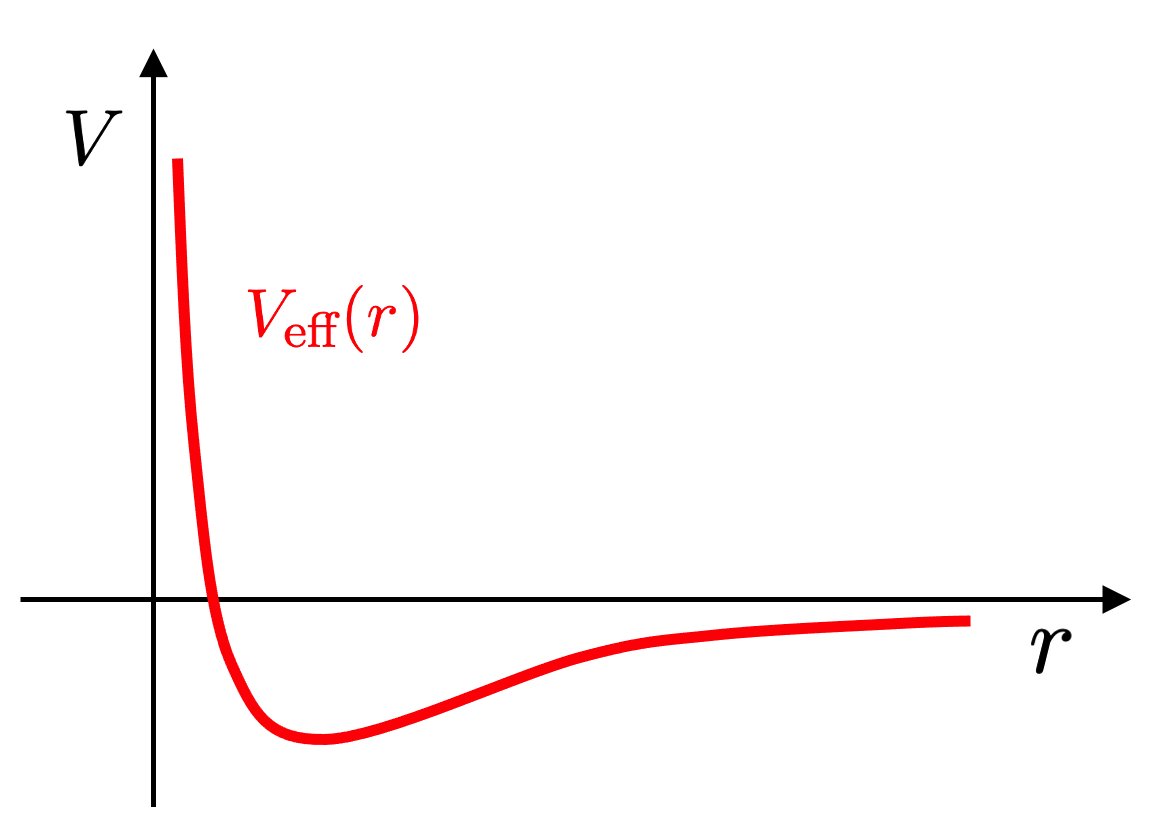
\includegraphics[width=0.45\linewidth]{images/Effective_potential.png}
    \caption{Behaviour or the effective potential; the repulsive part for low values of $r$ is associated to the angular component, the attractive part for high values of $r$ is associated to the electric part.}
    \label{fig:eff_potential}
\end{figure}

\begin{figure}[h!]
\centering
    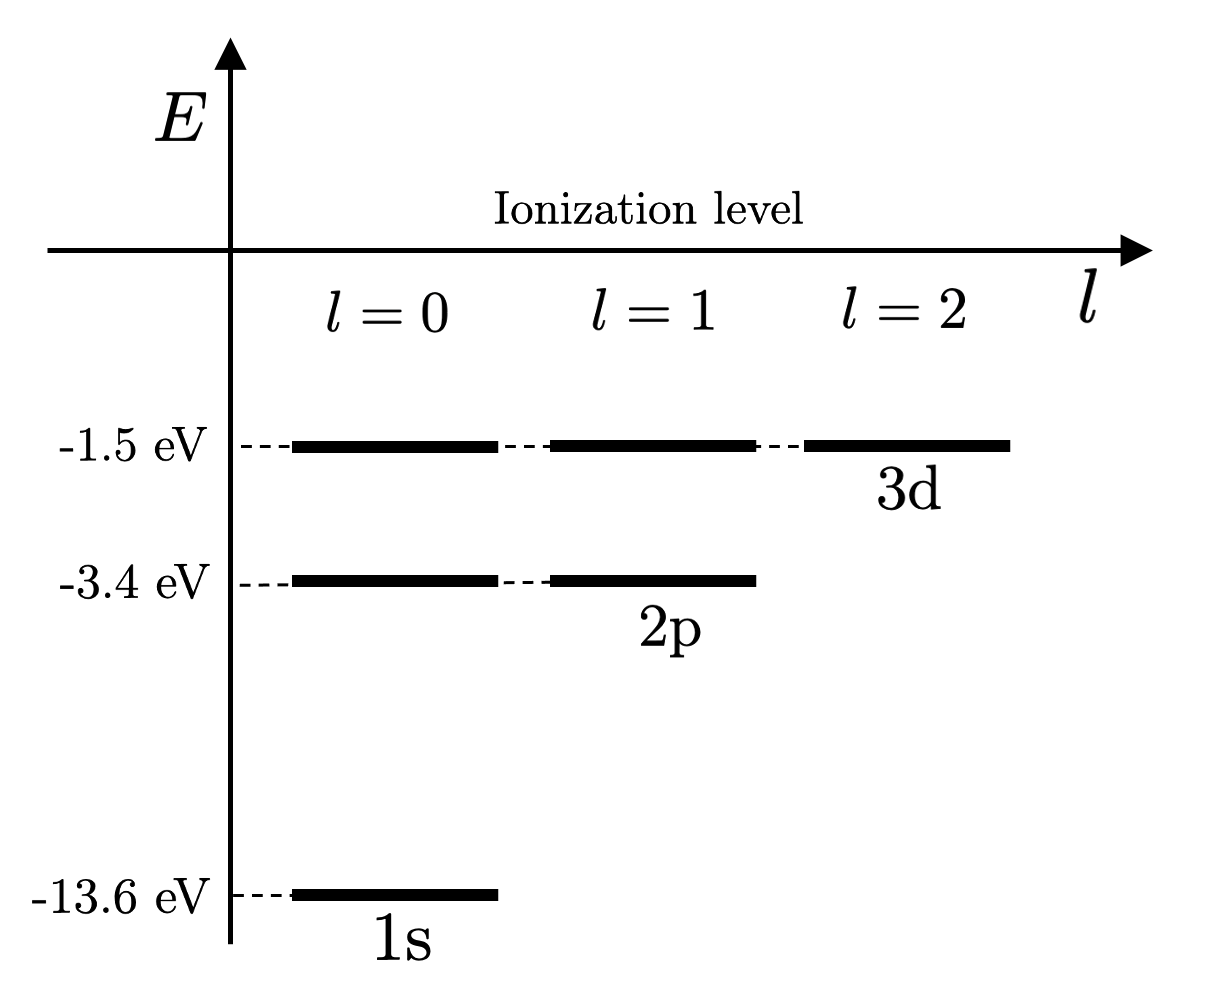
\includegraphics[width=0.5\linewidth]{images/Hydrogen_spectrum.png}
    \caption{First levels of the Hydrogen electron spectrum with the relative energies and orbital names.}
    \label{fig:hydro_spectrum}
\end{figure}

\subsection{Alkali atoms}

\begin{figure}[t]
\centering
    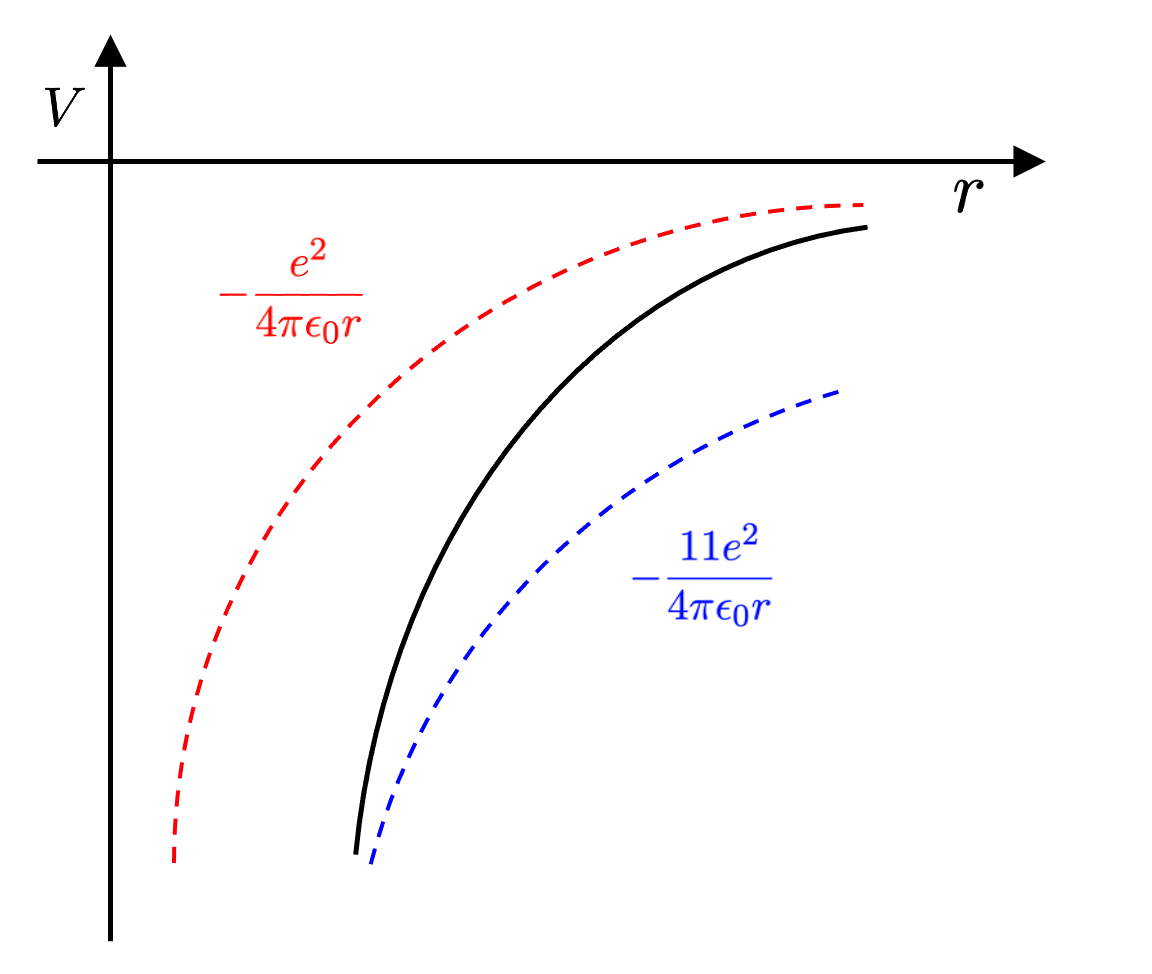
\includegraphics[width=0.58\linewidth]{images/Alkali_potential.png}
    \caption{Potential felt by the outer electron of a Sodium atom; for small distances an additional attractive term with respect to the Hydrogen potential is present and the total potential is shifted down, while for large distances the electron sees only the potential of a Hydrogen core.}
    \label{fig:pot_Alkali}
\end{figure}

\begin{figure}[b]
\centering
    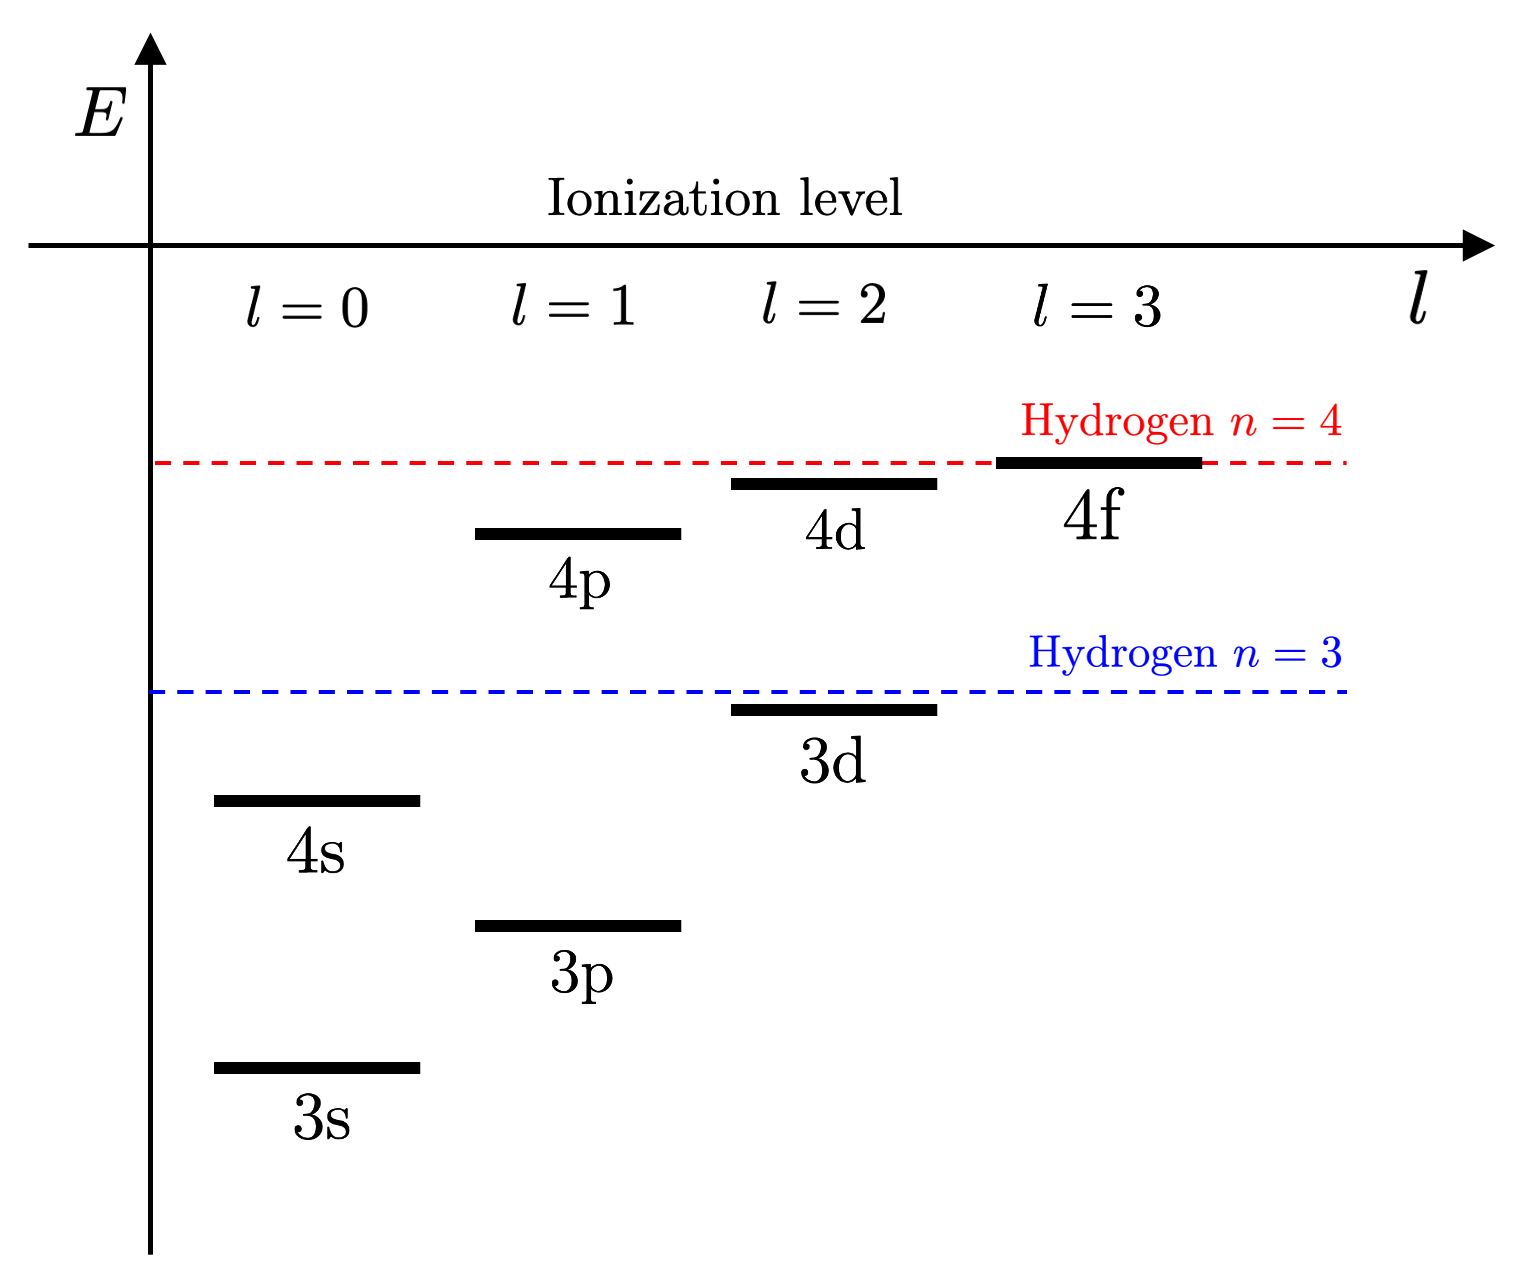
\includegraphics[width=0.61\linewidth]{images/Alkali_spectrum.png}
    \caption{First levels of the Sodium electron spectrum with the relative energies and orbital names; also the reference energies from the Hydrogen spectrum are reported.}
    \label{fig:alkali_spectrum}
\end{figure}


Hydrogen atoms are not used in everyday applications because they are light and volatile at temperatures little higher than the absolute zero. To avoid this, heavier atoms, like Alkali and in particular $^{11} \text{Na}_{\sim 22}$, are used. 

\noindent The Hamiltonian associated to these atoms is
\begin{equation}
    H_\text{Alkali} = \sum_{j} \left( - \frac{\hbar^2}{2m} \nabla_j^2 - \frac{Ze^2}{4 \pi \epsilon_0 \left| \Vec{r}_j\right|}\right) + \sum_{j\neq j'} \frac{e^2}{4 \pi \epsilon_0 \left| \Vec{r}_j - \Vec{r}_{j'}\right|}, 
    \label{eq:alkali_hamiltonian}
\end{equation}
where the summations are performed over the electrons. It can be be rewritten in many better ways, through some approximations. One could express $H_\text{Alkali}$ using the \textit{Hartree-Fock approximation}, but the entanglement information would be lost, due to the fact that this approximation provides the use of the \textit{mean field}.

Another possibility is the \textit{Shell model approximation}, which is a harsher approximation with respect to the previous one: the idea is that every electron sees only the core screened by the previous electrons. The behaviour of this potential for the outer electron of Sodium atom is reported in figure \ref{fig:pot_Alkali}. This model also gives a good explanation of the energy shift for atomic orbitals observed in alkali atoms with respect to the Hydrogen levels (figure \ref{fig:alkali_spectrum}); indeed, shifting momentarily towards a semi-classical picture with the electron as a proper particle orbiting around the nucleus, one could imagine that two processes take place:
\begin{itemize}
    \item as the electron gets closer to the nucleus, the electrostatic potential is stronger and the energy shift more pronounced;
    \item electrons with higher $l$ number experience a stronger centrifugal potential, bringing them farther away from the nucleus, resulting in a weaker electrostatic attraction and smaller energy shift.
\end{itemize}



\section{Interaction of Alkali atoms with light}
The interaction between charged particles and the electromagnetic field is governed by the Lorentz force $\Vec{F_L}=q(\Vec{E}+\Vec{v}\cross\Vec{B})$. The Lagrangian of a system where this is the only force in play is 
\begin{equation*}
    L(\Vec{r}, \Dot{\Vec{r}}, t)=\frac{1}{2} m \Dot{r}^2 + q \Dot{\Vec{r}}\cdot\Vec{A}- q \phi,
\end{equation*}
where the last part is equivalent to $J_\mu A^\mu$ in relativistic notation. Moving to the Hamiltonian view, since the canonical momentum is defined as 
\begin{equation*}
    p_i=\frac{\partial L}{\partial \Dot{\Vec{r}}} \qquad \implies \qquad \Vec{p}=m\Dot{\Vec{r}}+q\Vec{A}. 
\end{equation*}
The Hamiltonian in this \textit{minimal coupling} case can thus be written as 
\begin{equation}
    H= \frac{(\Vec{p}-q\Vec{A})^2}{2m}+q\phi, 
    \label{eq:Hatomlight}
\end{equation}
where both the part relative to the motion of the atom and the one associated to the interaction with light are present. 

\subsection{Power-Zienau transformation}

When using light at wavelengths such that $k^{-1}\gg a_0$ (where $a_0$ is the Bohr radius, i.e. the average of the electron-nucleus distance), as is the case with visible light, 
\begin{align*}
    \Vec{A}(\Vec{r}, t) \qquad \longrightarrow \qquad \Vec{A}({0}, t).
\end{align*}
This means that if the light wavelength is much larger than the interaction region (approximated by $a_0$), the vector potential is expected to vary little enough to be approximated with its central value. Within this approximation, which is called \textit{long-wavelength approximation}, $\Vec{A}$ commutes with momentum $\vec{p}$, since it no longer depends on position, i.e.
\begin{align*}
    \left[\vec{A}(\vec{r}),\, \vec{p} \right] \neq 0 \qquad \qquad  \left[\vec{A}(0),\, \vec{p} \right] = 0.
\end{align*}

% Power-Zienam transformation
The atom-light Hamiltonian (\ref{eq:Hatomlight}) can be rewritten by defining an unitary operator, the \textit{Power-Zienau transformation}
\begin{equation*}
    T = \exp{-\frac{i}{\hbar} q \, \Vec{r}\cdot\Vec{A}(0)}
\end{equation*}
and by using the using Hadamard's lemma
\begin{align*}
    e^{-S} \, B \,e^S = B+[S,B]+\frac{1}{2} [S,[S,B]]+...~
\end{align*}
to evaluate $H_{AL}'= T \, H_{AL} \, T^\dagger$. The first step consists of evaluating
\begin{align*}
    \Vec{p}\,'&=T\,\Vec{p}\,\,T^\dagger=\Vec{p}-\frac{i}{\hbar} q \left[\Vec{r}\cdot\Vec{A}(0), \, \Vec{p}\right] - \frac{q^2}{2\hbar^2} \left[\Vec{r}\cdot\Vec{A}(0),\left[\Vec{r}\cdot\Vec{A}(0),\Vec{p}\right]\right]+... = \\
    &=\Vec{p}-\frac{i}{\hbar} q \Vec{A}(0) \, \left[\Vec{r},\,\Vec{p}\right]=\Vec{p}+q\Vec{A},
\end{align*}
given that $[\Vec{r}, \, \Vec{p}]=i\hbar \mathbb{1}$ and thus all higher-order commutators are null. Therefore, 
\begin{equation*}
    T (\Vec{p}-q\Vec{A})^2 T^\dagger = T (\Vec{p}-q\Vec{A}) T^\dagger \, T (\Vec{p}-q\Vec{A}) T^\dagger = (\vec{p} + q \vec{A} - q \vec{A}) \cdot \vec{p} = p^2,
\end{equation*}
because $\vec{A}'(0) = T \vec{A}(0) T^\dagger = \vec{A}(0)$. Since $\phi'(\vec{r}) = T \phi(\vec{r}) T^\dagger = \phi(\vec{r})$, the final expression for $H_{AL}$ is
\begin{align}
    H'_{AL} = T H_{AL} T^\dagger = \frac{p^2}{2m} + q \phi. 
\end{align}

\subsection{Dipole approximation}
\label{dipole}

The same transformation can be applied to the Hamiltonian of the electromagnetic field $H_\text{light} \equiv H_{EM}$, treated in the previous chapter. In particular, using the Hadamard's relation 
\begin{align*}
    H'_{EM} &= T H_{EM} T^\dagger = \\
    &= H_{EM} - \frac{i}{\hbar} q \left[\vec{r} \cdot \vec{A}(0), \, H_{EM} \right] - \frac{q^2}{2\hbar^2} \left[ \vec{r} \cdot \vec{A}(0), \, \left[  \vec{r} \cdot \vec{A}(0), H_{EM} \right]\right] + ... = \\ 
    &= H_{EM} - \frac{i}{\hbar} {r_i} \left[ {A_i}(0), H_{EM}\right] - \frac{q^2}{2\hbar^2} r_i \, r_j \left[ A_i(0), \left[ A_j(0), H_{EM} \right] \right] + ..., 
\end{align*}
where the repeated indexes indicate a summation over the three components. Introducing the \textit{dipole operator} $\Vec{d}\equiv q\Vec{r},$ $H'_{EM}$ becomes 
\begin{equation}
    H'_{EM} = H_{EM} - \frac{i}{\hbar} d_i [A_i(0), H_{EM}]- \frac{1}{2\hbar^2} d_i d_j [A_i(0),[A_j(0), H_{EM}]]+ ...
    \label{eq:Hem1}
\end{equation}
The commutator in the previous expression is evaluated inserting the relation (\ref{eq:potvec}) for $\Vec{A}$ with $u(\Vec{r} = 0) \approx 1$:
\begin{align*}
    \left[\Vec{A}(0), H_{EM} \right] &= \sum_{\vec{k},\lambda} \sqrt{\frac{\hbar}{2 \varepsilon_0 \omega_k}} \frac{\vec{\epsilon}_\lambda}{\sqrt{V}} \left[ \left(a_{\vec{k},\lambda} + a_{\vec{k},\lambda}^\dagger\right), H_{EM}\right] = \\
    &= \sum_{\vec{k},\lambda} \sqrt{\frac{\hbar}{2 \varepsilon_0 \omega_k}} \frac{\vec{\epsilon}_\lambda}{\sqrt{V}} \left[ \left(a_{\vec{k},\lambda} + a_{\vec{k},\lambda}^\dagger\right), \sum_{\vec{k}',\lambda'} \hbar \omega_{k'} a_{\vec{k}',\lambda}'^\dagger a_{\vec{k}',\lambda'} \right] = \\
    &= \sum\limits_{\substack{\Vec{k},\lambda, \\ \Vec{k}', \lambda'}}
    \sqrt{\frac{\hbar}{2\epsilon_0\omega_k}} \frac{\Vec{\epsilon}_\lambda}{\sqrt{V}} \hbar\omega_{k'} \left(\left[a_{\Vec{k},\lambda}^\dagger, n_{\Vec{k'},\lambda'}\right]+\left[a_{\Vec{k},\lambda}, n_{\Vec{k'},\lambda'}\right]\right)=\\
    &=\hbar \sum_{\Vec{k}, \lambda} \sqrt{\frac{\hbar\omega_k}{2\epsilon_0}}~ \frac{\Vec{\epsilon}_{\Vec{k}}}{\sqrt{V}} \left(a_{\Vec{k},\lambda}-a_{\Vec{k},\lambda}^\dagger\right)= -i\hbar \Vec{E}(0),
\end{align*}
where the commutators are evaluated as 
\begin{align*}
    \left[a_{\Vec{k},\lambda}^\dagger, n_{\Vec{k'},\lambda'}\right] &= -a_{\vec{k},\lambda}^\dagger \delta_{\vec{k},\vec{k}'} \delta_{\lambda,\lambda'} \\
    \left[a_{\Vec{k},\lambda}, n_{\Vec{k'},\lambda'}\right] &= a_{\vec{k},\lambda} \delta_{\vec{k},\vec{k}'} \delta_{\lambda,\lambda'}
\end{align*}
Then (\ref{eq:Hem1}) becomes 
\begin{align}
    H'_{EM} = H_{EM} - d_i \, E_i(0) - \frac{i}{2 \hbar} d_i d_j \left[ A_i(0), E_j(0)\right] \equiv H_{EM} - \vec{d} \cdot \vec{E}(0) + H_{dd}. 
\end{align}
\\
%where other terms vanish since $[A_i,E_j] = 0$ for $i \neq j$ because 
%\begin{align*}
%    [\Vec{A},\Vec{E}] \propto \left[a_{\Vec{k},\lambda} + a_{\Vec{k},\lambda}^\dagger, a_{\Vec{k'},\lambda'}-a_{\Vec{k'},\lambda'}^\dagger\right] \sim -2 \left[a_{\Vec{k},\lambda}, a_{\Vec{k},\lambda}^\dagger\right] \delta_{\Vec{k}, \Vec{k'}}\delta_{\lambda, \lambda'} \sim -2 \delta_{\Vec{k}, \Vec{k'}}\delta_{\lambda, \lambda'}
%\end{align*}
%is no longer dependent on the field operators, the higher commutators are all zero;  moreover, the second term only operates on the atom degrees of freedom via the dipole operators, resulting in a shift of the atom levels.

The complete Hamiltonian which takes into account the light and the light-matter interaction contributions after the considered transformation is 
\begin{equation}
    H = \frac{p^2}{2m}+ q\phi +H_{dd} + H_{EM} - \Vec{d}\cdot\Vec{E}(0) \equiv H_\text{atom} + H_\text{light} + H_\text{atom-light}
    \label{eq:Hamfin}
\end{equation}
The first three terms define the total atom Hamiltonian, whose eigenstates are written as $\ket{n,l,m}$, the fourth is the light contribution, with eigenstates given by the Fock states, and the last is the first-order approximation for the atom-light interaction Hamiltonian. Higher orders can be obtained using further terms in the multipole expansion for $\Vec{A}$, i.e.
\begin{align*}
    \Vec{A}(\Vec{r}) = \Vec{A}(\Vec{0})+ r_i \frac{\partial}{\partial x_i} \Vec{A}+\frac{1}{2} r_i r_j \frac{\partial^2}{\partial x_i \partial x_j} \Vec{A}+ ... 
\end{align*}

\subsection{Selection rules}

Some considerations can be done about the dipole operator $\vec{d} = q \vec{r}$ which enters in the Hamiltonian for light-atom interaction. 

\subsubsection{Diagonal elements}
Under the \textit{parity transformation} $\Tilde{R}$ defined as
\begin{align*}
    \Tilde{R}\,\psi(x,y,z)&=\psi(-x, -y, -z) \\
    \Tilde{R}\psi(r, \theta, \varphi)&=\psi(r, \pi-\theta, \pi+\varphi),
\end{align*}
with $\Tilde{R}^\dagger=\Tilde{R}^{-1}=\Tilde{R}$, one has
\begin{align*}
    \Tilde{R}\, \Vec{r} \, \Tilde{R}^\dagger =-\Vec{r} \qquad &\Longleftrightarrow \qquad \{ \Tilde{R},\,  \vec{r} \} = 0, \\
    \Tilde{R}\, \Vec{p} \, \Tilde{R}^\dagger =-\Vec{p} \qquad &\Longleftrightarrow \qquad \{ \Tilde{R}, \, \vec{p} \} = 0, \\
     \Tilde{R}\, \Vec{L} \, \Tilde{R}^\dagger =\vec{L} \qquad &\Longleftrightarrow \qquad [ \Tilde{R}, \, \vec{p} ] = 0. \\
\end{align*}
Therefore, $\vec{L}$, $L^2$ and $L_z$ share the eigenbasis $\ket{n,l,m}$; in particular, the eigenvalues for $\Tilde{R}$ are 
\begin{align}
    \Tilde{R}\ket{n,l,m} =  (-1)^l \ket{n,l,m} \equiv e^{i \phi_{l,m}} \ket{n,l,m}
\end{align}
Therefore,
\begin{align*}
    \bra{n,l,m}\Vec{r}\ket{n,l,m} &= \bra{n,l,m} \Tilde{R}^\dagger \Tilde{R}  \Vec{r} \ket{n,l,m} = \\
    &= - \left( \bra{n,l,m} \tilde{R}^\dagger \right) \vec{r} \left( \tilde{R} \ket{n,l,m}\right) =\\
    &= -\bra{n,l,m} \vec{r} \ket{n,l,m}, 
\end{align*}
from which one deduces that the diagonal elements must all be zero.
\begin{equation*}
    \bra{n,l,m}{\Vec{r}}\ket{n,l,m}=0.
\end{equation*}

\subsubsection{Selection rules on $l$}
From the canonical commutators one can derive the identity
\begin{equation*}
    \left[L^2,\left[L^2, \vec{r}\right]\right]=2\hbar^2 \bigl\{\vec{r}, L^2\bigr\}.
\end{equation*}
Multiplying this by $\bra{n_1,l_1,m_1}$ on the left and by $\ket{n_2,l_2,m_2}$ on the right of both sides and bringing everything to the left one gets:
\begin{align*}
    \hbar^4\Bigl((l_1(l_1+1))^2-2l_1(l_1+1)l_2(l_2+1)+(l_2(l_2+1))^2~+\\ 
    -~2l_1(l_1+1)-2l_2(l_2+1)\Bigr)\bra{n_1,l_1,m_1}\Vec{r}\ket{n_2,l_2,m_2} = 0,
\end{align*}
which can be factorized in
\begin{equation*}
    (l_1-l_2+1)(l_1-l_2-1)(l_1+l_2)(l_1+l_2+2)\bra{n_1,l_1,m_1}\Vec{r}\ket{n_2,l_2,m_2} = 0.
\end{equation*}
The last two parenthesis are irrelevant since they can not be null, hence from the first two one has that the only case in which the matrix element can be nonzero is when $\Delta l= l_1 - l_2 =\pm1$. This is a necessary, not sufficient, condition.

\subsubsection{Selection rules on $m$}
In order to obtain a similar relation for the quantum number $m$, one can assume that the electric field is along the $z-$axis and two cases are considered: 
\begin{itemize}
    \item \textbf{Case $\vec{\epsilon} \parallelslant \hat{z}$} \\
    Since $[L_z, r_z]=0$, one immediately gets
    \begin{equation*}
    \bra{n_1,l_1,m_1}[L_z,\Vec{r}]\ket{n_2,l_2,m_2} = 
        0 = \hbar(m_1-m_2)\bra{n_1,l_1,m_1}\Vec{r}\ket{n_2,l_2,m_2} \;\;.
    \end{equation*}
    Thus the matrix element can be nonzero when $\Delta m = m_1 - m_2 =0$. 
    \item \textbf{Case $\vec{\epsilon} \perp \hat{z}$} \\
    Since $[L_z, r_x ]= i\hbar y$ and $[L_z, r_y]=-i\hbar x$, which implies $[L_z, x\pm iy]=\pm\hbar(x\pm iy)$, one gets
    \begin{align*}
        \bra{n_1,l_1,m_1} \left( [L_z, x\pm iy] \mp \hbar(x\pm iy) \right) \ket{n_2,l_2,m_2} = 0
    \end{align*}
    from which
    \begin{align*}
        \hbar(m_1-m_2-1)\bra{n_1,l_1,m_1}(x+iy)\ket{n_2,l_2,m_2} &= 0, \\
        \hbar(m_1-m_2+1)\bra{n_1,l_1,m_1}(x-iy)\ket{n_2,l_2,m_2} &= 0.
    \end{align*}
    Thus the matrix element can be null when the coefficients are null, hence $\Delta m = m_1 - m_2 = \pm 1$. It can be shown that the $+1$ case corresponds to left-handed circularly polarized light, while the $-1$ case corresponds to right-handed light.
\end{itemize}

An example of the application of this selection rules is given in figure (\ref{fig:sodium_spectrum}), in which the allowed transitions for the lowest level of Sodium spectrum are reported.  

\begin{figure}[h]
\centering
    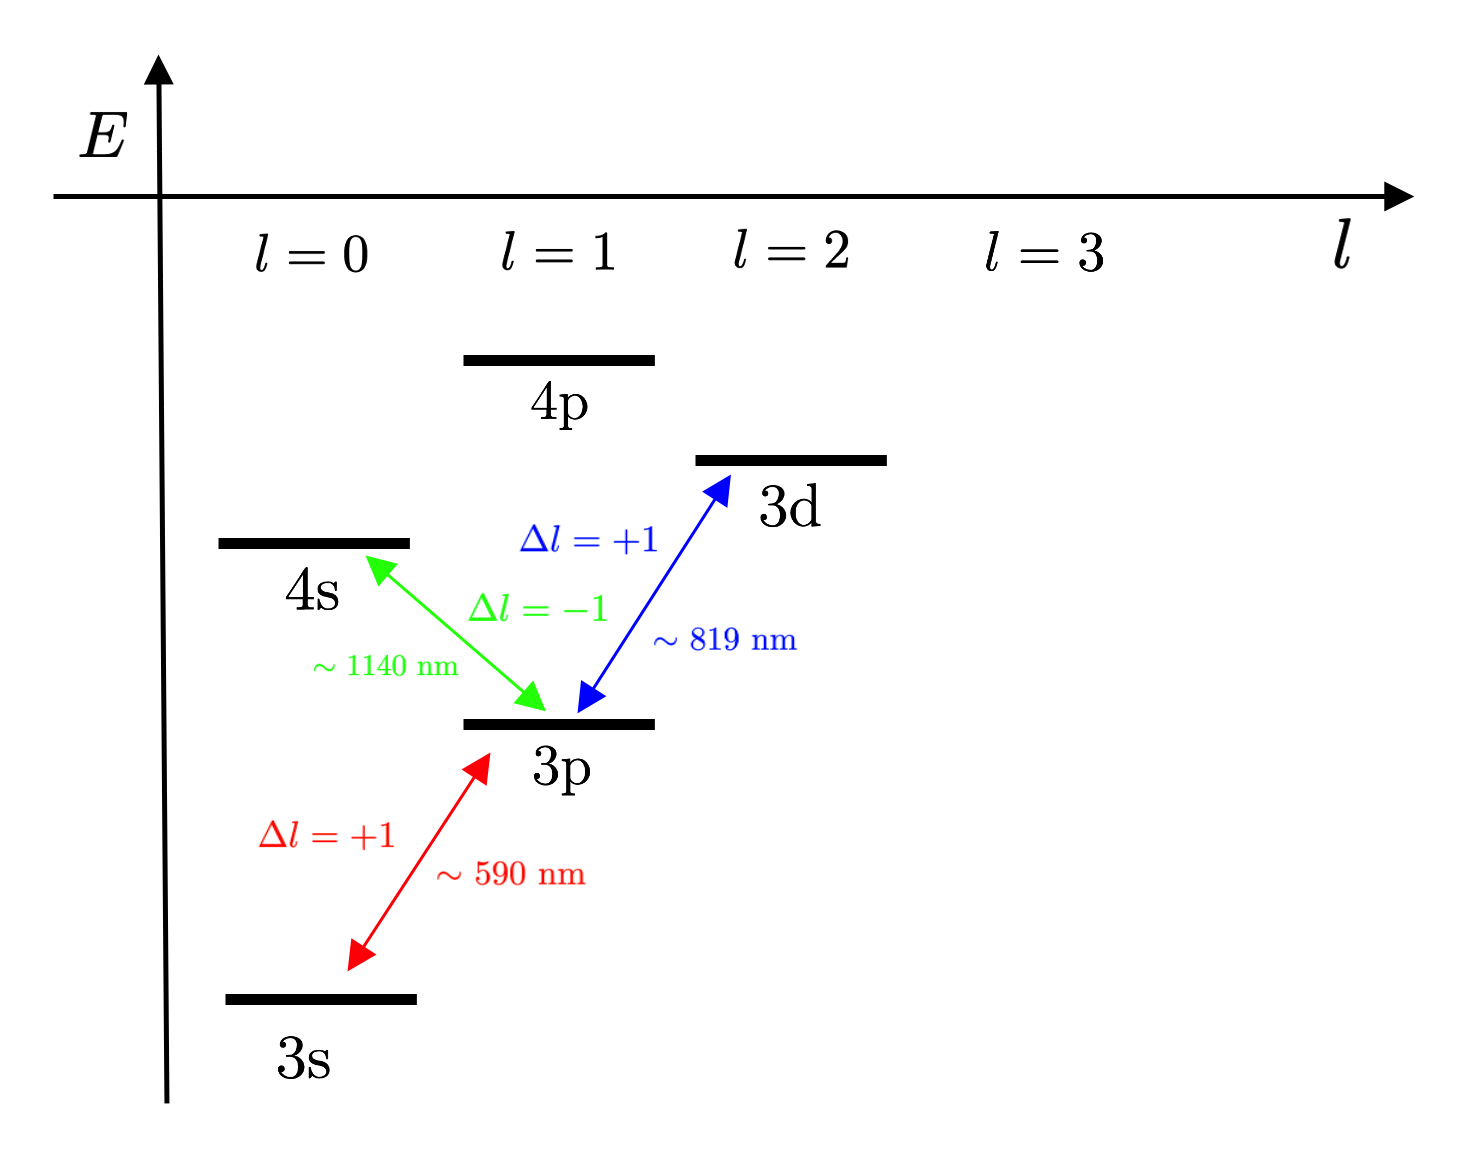
\includegraphics[width=0.7\linewidth]{images/Sodium_transition.png}
    \caption{First levels of the Sodium electron spectrum with the allowed transitions and the relative wavelengths.}
    \label{fig:sodium_spectrum}
\end{figure}






\section{Lifting energy-level degeneracy}

The Hamiltonian for the outer electron of an Hydrogen-like atom can be written as
\begin{align*}
    H = \frac{p^2}{2m} + V_\text{eff}, 
\end{align*}
where:
\begin{align*}
        V_\text{eff} = - \frac{e^2}{4 \pi \varepsilon_0 r} \qquad &\text{for the Hydrogen atoms;} \\
        V_\text{eff} = - \frac{Z_\text{eff} e^2}{4 \pi \varepsilon_0 }\left( \frac{1}{r} - \mathcal{C}(r)\right) 
    \qquad &\text{with $Z_\text{eff} = 1$ for the neutral alkali atoms} \\
    &\text{or $Z_\text{eff} = 2$ for single-charged alkali-earth ions.}
\end{align*}
The term $\mathcal{C}(r)$ is a corrective term which is relevant for lower $l$. 
The energy levels are 
\begin{align*}
    E_{n,l} &= - \frac{m_e e^4 Z_\text{eff}^2}{2 (4 \pi \varepsilon_0)^2 \hbar^2} \left( \frac{1}{n^2} + \tilde{\mathcal{C}}_{n,l}(r)\right) = \\
    & = -\frac{m_e c^2}{2} Z_\text{eff}^2 \underbrace{\left( \frac{e^2}{4 \pi \varepsilon_0 \hbar c}\right)^2}_{\alpha^2} \left( \frac{1}{n^2} +  \tilde{\mathcal{C}}_{n,l}(r) \right),
\end{align*}
where $Z_\text{eff}$ is the residual charge at the outer shell and $\alpha$ is the fine structure constant. From the last expression, one can notice that the degeneracy in $n$ and $l$ is resolved. Nevertheless in many applications it is useful to have complete resolved energy levels and to obtain this situation the quantum numbers $m$ and $s_z$ are taken into account. In particular, the effects studied to remove this degeneracy are two:
\begin{itemize}
    \item \textit{Spin-orbit coupling}: it is an effect already present in the studied atoms and it derives from the fine structure; 
    \item \textit{Zeeman effect}: it derives from the application of an external magnetic field. 
\end{itemize}


\subsection{Spin-orbit coupling}

%\begin{center}
%

\tikzset{every picture/.style={line width=0.75pt}} %set default line width to 0.75pt        

\begin{tikzpicture}[x=0.75pt,y=0.75pt,yscale=-1,xscale=1]
%uncomment if require: \path (0,125); %set diagram left start at 0, and has height of 125

%Flowchart: Connector [id:dp31225744112714693] 
\draw   (13.33,83.21) .. controls (13.33,67.63) and (61.21,55) .. (120.27,55) .. controls (179.32,55) and (227.2,67.63) .. (227.2,83.21) .. controls (227.2,98.78) and (179.32,111.41) .. (120.27,111.41) .. controls (61.21,111.41) and (13.33,98.78) .. (13.33,83.21) -- cycle ;
%Shape: Boxed Line [id:dp7490815418622135] 
\draw    (120.56,49.41) -- (120.53,12.74) ;
\draw [shift={(120.53,10.74)}, rotate = 89.96] [color={rgb, 255:red, 0; green, 0; blue, 0 }  ][line width=0.75]    (10.93,-3.29) .. controls (6.95,-1.4) and (3.31,-0.3) .. (0,0) .. controls (3.31,0.3) and (6.95,1.4) .. (10.93,3.29)   ;
%Shape: Circle [id:dp30161062782824144] 
\draw  [fill={rgb, 255:red, 0; green, 0; blue, 0 }  ,fill opacity=1 ] (222.27,83.21) .. controls (222.27,81.03) and (224.03,79.27) .. (226.2,79.27) .. controls (228.37,79.27) and (230.13,81.03) .. (230.13,83.21) .. controls (230.13,85.38) and (228.37,87.14) .. (226.2,87.14) .. controls (224.03,87.14) and (222.27,85.38) .. (222.27,83.21) -- cycle ;
%Shape: Ellipse [id:dp5616793906082976] 
\draw   (103.17,81.21) .. controls (103.17,76.99) and (110.82,73.58) .. (120.27,73.58) .. controls (129.71,73.58) and (137.37,76.99) .. (137.37,81.21) .. controls (137.37,85.42) and (129.71,88.83) .. (120.27,88.83) .. controls (110.82,88.83) and (103.17,85.42) .. (103.17,81.21) -- cycle ;
%Shape: Ellipse [id:dp7473632087803942] 
\draw   (108.95,94.03) .. controls (105.79,91.24) and (108.3,83.24) .. (114.55,76.16) .. controls (120.8,69.08) and (128.42,65.6) .. (131.58,68.38) .. controls (134.74,71.17) and (132.23,79.17) .. (125.98,86.25) .. controls (119.73,93.33) and (112.11,96.81) .. (108.95,94.03) -- cycle ;
%Shape: Ellipse [id:dp36775889518050264] 
\draw   (108.05,69.24) .. controls (111,66.23) and (118.86,69.15) .. (125.6,75.76) .. controls (132.35,82.37) and (135.43,90.17) .. (132.48,93.17) .. controls (129.53,96.18) and (121.68,93.26) .. (114.93,86.65) .. controls (108.18,80.04) and (105.11,72.24) .. (108.05,69.24) -- cycle ;

% Text Node
\draw (127.33,24.07) node [anchor=north west][inner sep=0.75pt]  [font=\small]  {$L$};
% Text Node
\draw (234,68.07) node [anchor=north west][inner sep=0.75pt]  [font=\footnotesize]  {$e^{-}$};
% Text Node
\draw (139.37,84.61) node [anchor=north west][inner sep=0.75pt]  [font=\small]  {$Z_{\text{eff}}$};


\end{tikzpicture}
%\end{center}

Consider the an Hydrogen-like atom in a laboratory frame in absence of magnetic fields and imagine that the outer electron moves with velocity $\vec{v}$. If the problem is studied from the frame in which the electron is at rest, the latter experiences an effective magnetic field
\begin{align}
    \vec{B}_{el} = -\frac{1}{c^2} \vec{v} \times \vec{E}, 
    \label{eq:B}
\end{align}
where $\vec{E}$ is the core electric field measured in the laboratory frame. Since $\vec{E}$ is radial, one can write 
\begin{align*}
    \vec{E} = \frac{\vec{\nabla}V}{e} = \frac{\vec{r}}{e {r}} \frac{\partial V_\text{eff}}{\partial r} , 
\end{align*}
while $\vec{v} = \vec{p}/m_e$ (in non-relativistic approximation). Therefore, equation (\ref{eq:B}) becomes
\begin{align}
    \vec{B}_{el} = -\frac{1}{c^2} \left( \frac{\vec{p}}{m_e} \times \vec{r} \right) \frac{1}{e {r}} \frac{\partial V_\text{eff} }{\partial r} = \frac{1}{e m_e c^2 r} \frac{\partial V_\text{eff}}{\partial r}  \vec{L}, 
\end{align}
where $\vec{L}$ is the angular momentum in the laboratory frame. \\

This magnetic field can couple with the magnetic dipole moment associated to the electron spin, given by 
\begin{align*}
    \vec{\mu}_s = -\frac{e}{2 m_e} g_s \vec{S} = -\mu_B g_s \vec{S},  
\end{align*}
where $g_s$ is the electron $g$-factor ($g_s = 2$ from Dirac free theory) and $\mu_B = e\hbar/(2 m_e)$ is the Bohr magneton. In particular, the additional term to the Hamiltonian of the electron evaluated in the electron reference frame is 
\begin{align}
    H_\text{spin-orbit}^{el} \equiv H_{SO}^{el} = - \vec{\mu}_s \cdot \vec{B}_{el} = \frac{\mu_B g_s}{e m c^2 \hbar} \left( \frac{1}{r} \frac{\partial V_\text{eff}}{\partial r} \right)\vec{S} \cdot \vec{L}. 
\end{align}
The following step consists of returning to the laboratory frame. The explicit calculation leads to the following terms 
\begin{align}
    H_\text{spin-orbit}^{lab} \equiv H_{SO}^{lab} = \frac{\mu_B (g_S-1)}{e m c^2 \hbar} \left( \frac{1}{r} \frac{\partial V_\text{eff}}{\partial r} \right)\vec{S} \cdot \vec{L}. 
\end{align}
Using the general expression for $V_\text{eff}$ presented above, the spin-orbit Hamiltonian is 
\begin{align}
    H_{SO}^{lab} = \frac{\mu_B (g_S-1)Z_\text{eff} e}{4 \pi \varepsilon_0 m c^2 \hbar} \left( \frac{1}{r^3} - \frac{\partial \mathcal{C}}{\partial r} \right) \vec{S} \cdot \vec{L}, 
\end{align}
or more in general (omitting the reference to the laboratory frame)
$$H_{SO} = \Bigl( \textrm{some function of } r\Bigr) \; \vec{L}\cdot\vec{S}.$$
The basis formed by elements like $\ket{l,m,s,s_z}$ does not diagonalize this Hamiltonian. In order to do this, one has to introduce the \textit{total angular momentum}
\begin{align}
    \vec{J} = \vec{L} + \vec{S} 
\end{align}
and the new useful basis becomes $\ket{l,s,j,j_z}$ (indeed $L^2$, $S^2$, $J^2$ and $J_z$ commute). Hence from 
\begin{align*}
    \begin{pmatrix}
    L^2 \\ L_z \\ S^2 \\ S_z 
    \end{pmatrix}
    \ket{l,m,s,s_z} = 
    \begin{pmatrix}
    \hbar^2 l(l+1) \\ \hbar m \\ \hbar^2 s(s+1) \\ \hbar s_z 
    \end{pmatrix}
    \ket{l,m,s,s_z} 
\end{align*}
one passes to 
\begin{align*}
    \begin{pmatrix}
    L^2 \\ S^2 \\ J^2 \\ J_z 
    \end{pmatrix}
    \ket{l,s,j,j_z} = 
    \begin{pmatrix}
    \hbar^2 l(l+1) \\ \hbar^2 s(s+1) \\  \hbar^2 j(j+1) \\ \ \hbar j_z 
    \end{pmatrix}
    \ket{l,s,j,j_z}
\end{align*}
with 
\begin{align*}
    j = l +\dfrac{1}{2}, l - \dfrac{1}{2} \qquad \text{and} \qquad j_z = -j, ..., j.
\end{align*}
In principle, one should evaluate the Clebsch-Gordan coefficient to move from one basis to another, but in this case a simpler approach is used. \\
The term $\vec{L} \cdot \vec{S}$ in $H_{SO}$ can be rewritten by noticing that
\begin{align*}
{J}^2 & = (\vec{L} + \vec{S})^2 = {S}^2 + {L}^2 + \vec{S}\cdot\vec{L} + \vec{L}\cdot\vec{S} = {S}^2 + {L}^2 + 2\vec{L}\cdot\vec{S},
\end{align*}
where the last equation is obtained from the fact that $\vec{L}$ and $\vec{S}$ commute because the operators act on different spaces. From this
\begin{equation*}
\vec{L}\cdot\vec{S} = \frac{1}{2}\left( {J}^2 - {L}^2 - {S}^2\right)
\end{equation*}
and hence 
\begin{align}
    H_{SO} \simeq \Bigl( \textrm{some function of } r\Bigr) \left( {J}^2 - {L}^2 - {S}^2\right), 
\end{align}
which is clearly diagonalized by $\ket{n,l,s,j,j_z}$. 

Once the new basis is found, the first-order degeneracy removing Hamiltonian is given by (\ref{eq:H1})
\begin{align*}
    H^{(1)} = \Pi_{n,l,s=1/2}\, H_{SO}  \, \Pi_{n,l,s=1/2} 
\end{align*}
while the associated energy shift is 
\begin{align*}
\Delta E_{{SO}}^{(1)} & = \bra{n,l,j,j_z} H_{SO} \ket{n,l,j,j_z} = \\
& \propto   \underbrace{ \bra{n,l}{\left( \frac{1}{r}\frac{\partial V_{\text{eff}}}{\partial r} \right)}\ket{n,l} }_{\text{just an integral $>$ 0}}  \left( j(j+1) - l(l+1) - \underbrace{s(s+1)}_{3/4} \right)
\end{align*}
This expression shows that some degeneracies are removed, as levels with same $l$ are now split by means of $j = l \pm \frac{1}{2}$. 
\begin{center}


\tikzset{every picture/.style={line width=0.75pt}} %set default line width to 0.75pt        

\begin{tikzpicture}[x=0.75pt,y=0.75pt,yscale=-1,xscale=1]
%uncomment if require: \path (0,84); %set diagram left start at 0, and has height of 84

%Straight Lines [id:da5451741662949235] 
\draw [line width=1.5]    (30,45) -- (75.97,45) ;
%Straight Lines [id:da037325881742858114] 
\draw [line width=1.5]    (100,30) -- (107.37,30) -- (145.97,30) ;
%Straight Lines [id:da1983425953314939] 
\draw [line width=1.5]    (100,60) -- (145.97,60) ;
%Straight Lines [id:da734262702937892] 
\draw    (75.97,45) -- (100,30) ;
%Straight Lines [id:da9010281726737945] 
\draw    (75.97,45) -- (100,60) ;

% Text Node
\draw (13,37.9) node [anchor=north west][inner sep=0.75pt]  [font=\small]  {$l$};
% Text Node
\draw (158,21.9) node [anchor=north west][inner sep=0.75pt]  [font=\small]  {$j=l+1/2$};
% Text Node
\draw (158,52.4) node [anchor=north west][inner sep=0.75pt]  [font=\small]  {$j=l-1/2$};


\end{tikzpicture}

\end{center}

A final note is about the fact that in this procedure the relativistic effects are neglected. Nevertheless, they do not determine, at this level, a splitting but a shift of all energy levels of the order of $2\pi/\alpha^2$. 


\begin{tcolorbox} [breakable, enhanced]
\textbf{Note about notation}\\ 
A state with quantum numbers $n, l, s, j$ is labelled as $$n^{2s+1}l_j$$
where $l$ is replaced with a capital letter according to its value. The first four values are associated to: 
\begin{align*}
l=0 \rightarrow S \qquad & l=1 \rightarrow P\\
l=2 \rightarrow D \qquad & l=3 \rightarrow F 
\end{align*}
For instance, $4^2S_{1/2}  \Longleftrightarrow \ket{n=4,l=0,s=1/2,j=1/2}$.
\end{tcolorbox}

\begin{tcolorbox} [breakable, enhanced]
\textbf{Fine structure of Sodium} ($Z=11$) \\
A partial lifting of the degeneracy in Sodium spectrum is reported below. The energy levels $3^2 P_{1/2}$ and $3^2 P_{3/2}$ are two-time and four-time degenerate, hence the degeneracy is only partially removed. 
\begin{center}


\tikzset{every picture/.style={line width=0.75pt}} %set default line width to 0.75pt        

\begin{tikzpicture}[x=0.75pt,y=0.75pt,yscale=-1,xscale=1]
%uncomment if require: \path (0,182); %set diagram left start at 0, and has height of 182

%Shape: Axis 2D [id:dp3017160538012129] 
\draw  (45.33,32.16) -- (324.2,32.16)(56.87,10.33) -- (56.87,167.43) (317.2,27.16) -- (324.2,32.16) -- (317.2,37.16) (51.87,17.33) -- (56.87,10.33) -- (61.87,17.33)  ;
%Straight Lines [id:da24085599967696059] 
\draw [line width=1.5]    (86,146) -- (146.47,146) ;
%Straight Lines [id:da1539316269981591] 
\draw [line width=1.5]    (166,96) -- (226.47,96) ;
%Straight Lines [id:da40743469547233857] 
\draw [line width=1.5]    (226,82.33) -- (286.47,82.33) ;
%Straight Lines [id:da6604133921274191] 
\draw  [dash pattern={on 0.84pt off 2.51pt}]  (56.2,87.67) -- (315.53,87.67) ;
%Straight Lines [id:da1648566831794681] 
\draw  [dash pattern={on 0.84pt off 2.51pt}]  (56,146) -- (86,146) ;
%Straight Lines [id:da12556235022798856] 
\draw    (167.92,100.57) -- (127.88,140.59) ;
\draw [shift={(126.47,142)}, rotate = 315.01] [color={rgb, 255:red, 0; green, 0; blue, 0 }  ][line width=0.75]    (6.56,-1.97) .. controls (4.17,-0.84) and (1.99,-0.18) .. (0,0) .. controls (1.99,0.18) and (4.17,0.84) .. (6.56,1.97)   ;
\draw [shift={(169.33,99.16)}, rotate = 135.01] [color={rgb, 255:red, 0; green, 0; blue, 0 }  ][line width=0.75]    (6.56,-1.97) .. controls (4.17,-0.84) and (1.99,-0.18) .. (0,0) .. controls (1.99,0.18) and (4.17,0.84) .. (6.56,1.97)   ;
%Straight Lines [id:da5918618746875237] 
\draw    (276.02,85.26) -- (144.05,140.38) ;
\draw [shift={(142.2,141.16)}, rotate = 337.33] [color={rgb, 255:red, 0; green, 0; blue, 0 }  ][line width=0.75]    (6.56,-1.97) .. controls (4.17,-0.84) and (1.99,-0.18) .. (0,0) .. controls (1.99,0.18) and (4.17,0.84) .. (6.56,1.97)   ;
\draw [shift={(277.87,84.49)}, rotate = 157.33] [color={rgb, 255:red, 0; green, 0; blue, 0 }  ][line width=0.75]    (6.56,-1.97) .. controls (4.17,-0.84) and (1.99,-0.18) .. (0,0) .. controls (1.99,0.18) and (4.17,0.84) .. (6.56,1.97)   ;

% Text Node
\draw (95,151.4) node [anchor=north west][inner sep=0.75pt]    {$3^{2} S_{1/2}$};
% Text Node
\draw (172.33,58.07) node [anchor=north west][inner sep=0.75pt]    {$3^{2} P_{1/2}$};
% Text Node
\draw (233,52.07) node [anchor=north west][inner sep=0.75pt]    {$3^{2} P_{3/2}$};
% Text Node
\draw (2.33,82.07) node [anchor=north west][inner sep=0.75pt]  [font=\footnotesize]  {$-3.04\ eV$};
% Text Node
\draw (1.67,141.07) node [anchor=north west][inner sep=0.75pt]  [font=\footnotesize]  {$-5.14\ eV$};
% Text Node
\draw (201.33,117.07) node [anchor=north west][inner sep=0.75pt]  [font=\footnotesize]  %{$589.0\ nm,\ 2.105\ eV$};
{$ \begin{array}{l}
589.0\ nm,\\
2.105\ eV
\end{array}$};
% Text Node
\draw (79.33,100.4) node [anchor=north west][inner sep=0.75pt]  [font=\footnotesize]  {$ \begin{array}{l}
589.6\ nm,\\
2.013\ eV
\end{array}$};


\end{tikzpicture}

\end{center}
\end{tcolorbox}

From the Sodium example it is evident that, to have a complete resolution of the energy levels, something different must be introduced. 

\subsection{Zeeman effect}

Consider the system described in the previous section with an external classical magnetic field $\vec{B}$. The interaction is described by the Hamiltonian
\begin{equation*}
H_B = -\vec{\mu}_s\cdot \vec{B} -\vec{\mu}_l\cdot \vec{B} = \frac{\mu_B}{\hbar} \left( g_s \vec{S} + g_l \vec{L}\right) \cdot \vec{B}
\label{eq:HB}
\end{equation*}
where
\begin{equation*}
g_s \simeq 2.0023 \qquad \text{and} \qquad g_l \simeq \frac{m_{\textrm{reduced}}}{m_{e^-}} = \frac{1}{1 + m_e/m_\text{reduced}}\lesssim 1
\end{equation*}
are the electron spin $g$-factor and the orbital $g$-factor respectively. 
In (\ref{eq:HB}), $\vec{\mu}_s$ is the spin magnetic dipole moment while $\vec{\mu}_l$ is the orbital magnetic dipole moment. 

To simplify even more, one can orient $\vec B$ along the $\vec{z}$ axis and hence 
\begin{equation*}
H_B = \frac{\mu_B}{\hbar} \left( 2S_z + L_z \right) B_z
\end{equation*} 


\subsubsection{Case 1: Strong $\vec B$ regime}

By ``strong $B$ regime" one refers to a situation in which the energies associated to the magnetic field are much bigger than those of spin-orbit, namely $\Delta E_B \gg \Delta E_{SO}$.

In this case, $n,l,m$ and $s_z$ are good quantum numbers and the computation of the energy shift is straightforward:
\begin{align*}
\Delta E_{n,l,m,s_z} &= \bra{n,l,m,s_z} H_B \ket{n,l,m,s_z} =\\
& = \frac{\mu_B B}{\hbar} \bra{n,l,m,s_z}  2S_z + L_z \ket{n,l,m,s_z} = \mu_B (2s_z + m)B
\end{align*}
In this regime, the splitting is called \textit{Paschen-Back effect}.

\begin{tcolorbox} [breakable, enhanced]
\textbf{Paschen-Back effect for a $P$ level}
\begin{center}
\tikzset{every picture/.style={line width=0.75pt}} %set default line width to 0.75pt        

\begin{tikzpicture}[x=0.75pt,y=0.75pt,yscale=-1,xscale=1]
%uncomment if require: \path (0,141); %set diagram left start at 0, and has height of 141

%Straight Lines [id:da8975336306251028] 
\draw    (41,70) -- (56.97,70) -- (86.97,70) ;
%Straight Lines [id:da28508596950100773] 
\draw [line width=0.75]    (120,20) -- (135.97,20) -- (165.97,20) ;
%Straight Lines [id:da44121474273875605] 
\draw [line width=0.75]    (120,45) -- (135.97,45) -- (165.97,45) ;
%Straight Lines [id:da8891350329962026] 
\draw [line width=0.75]    (120,70) -- (135.97,70) -- (165.97,70) ;
%Straight Lines [id:da31409125050054265] 
\draw [line width=0.75]    (120,95) -- (135.97,95) -- (165.97,95) ;
%Straight Lines [id:da3078724766520293] 
\draw [line width=0.75]    (120,120) -- (135.97,120) -- (165.97,120) ;
%Straight Lines [id:da21353385953707116] 
\draw  [dash pattern={on 0.84pt off 2.51pt}]  (86.97,70) -- (120,20) ;
%Straight Lines [id:da2989866705363874] 
\draw  [dash pattern={on 0.84pt off 2.51pt}]  (86.97,70) -- (120,120) ;
%Straight Lines [id:da6705557415835165] 
\draw  [dash pattern={on 0.84pt off 2.51pt}]  (86.97,70) -- (120,95) ;
%Straight Lines [id:da2096870206528575] 
\draw  [dash pattern={on 0.84pt off 2.51pt}]  (86.97,70) -- (120,70) ;
%Straight Lines [id:da22004352286960305] 
\draw  [dash pattern={on 0.84pt off 2.51pt}]  (86.97,70) -- (120,45) ;

% Text Node
\draw (14.33,62.07) node [anchor=north west][inner sep=0.75pt]  [font=\small]  {$P$};
% Text Node
\draw (172,13.4) node [anchor=north west][inner sep=0.75pt]  [font=\small]  {$\ket{\ 1,\ 1/2}$};
% Text Node
\draw (172,38.4) node [anchor=north west][inner sep=0.75pt]  [font=\small]  {$\ket{\ 0,\ 1/2}$};
% Text Node
\draw (172,63.4) node [anchor=north west][inner sep=0.75pt]  [font=\small]  {$\ket{\ 1,\ -1/2} ,\ \ket{-1,\ 1/2}$};
% Text Node
\draw (172,88.4) node [anchor=north west][inner sep=0.75pt]  [font=\small]  {$\ket{\ 0,\ -1/2}$};
% Text Node
\draw (172,113.4) node [anchor=north west][inner sep=0.75pt]  [font=\small]  {$\ket{-1,\ -1/2}$};
% Text Node
\draw (352,13.4) node [anchor=north west][inner sep=0.75pt]  [font=\scriptsize]  {$+2\mu _{B}$};
% Text Node
\draw (352,37.73) node [anchor=north west][inner sep=0.75pt]  [font=\scriptsize]  {$+\ \mu _{B}$};
% Text Node
\draw (352,63.4) node [anchor=north west][inner sep=0.75pt]  [font=\scriptsize]  {$+\ 0\ $};
% Text Node
\draw (352,88.4) node [anchor=north west][inner sep=0.75pt]  [font=\scriptsize]  {$-\ \mu _{B}$};
% Text Node
\draw (352,113.4) node [anchor=north west][inner sep=0.75pt]  [font=\scriptsize]  {$-2\mu _{B}$};


\end{tikzpicture}

\end{center}

The degeneracy of $\ket{m,s_z} = \ket{1, -1/2}, \ket{-1, 1/2}$ is eventually removed by relativistic effects.
\end{tcolorbox}

\subsubsection{Case 2: Weak $\vec B$ regime}

On the other hand, one might consider the range of energies in which $\Delta E_B \lesssim \Delta E_{SO}$; in this case, the quantum numbers $n,l,j$ and $j_z$ are used:
\begin{align*}
\Delta E_{n,l,j,j_z} & = \bra{n,l,j,j_z} H_B \ket{n,l,j,j_z} =\\
& = \frac{\mu_B B}{\hbar} \bra{n,l,j,j_z} g_sS_z + g_lL_z \ket{n,l,j,j_z} = \\
& = \frac{\mu_B B}{\hbar} \bra{n,l,j,j_z}  (g_s-g_l)S_z + g_lJ_z \ket{n,l,j,j_z} = \\
&= \frac{\mu_B B}{\hbar} \bigg[ (g_s-g_l)\bra{n,l,j,j_z}S_z\ket{n,l,j,j_z} + g_l\hbar j_z \bigg]
\end{align*}
From the last line, one notices that there is not a straightforward way to evaluate $\bra{n,l,j,j_z}S_z\ket{n,l,j,j_z}$ no eigenvector for $S_z$ are present. To compute this term one can use the \textit{projection theorem} according to which the expectation value of a quantity $\vec{A}$ that transforms as a vector can be written as
\begin{equation*}
\langle \vec A \rangle = \Bigl\langle \left(J^2\right)^{-1} \left( \vec{J}\cdot \vec{A}\right) \vec{J} \Bigr\rangle
\end{equation*}
Therefore
\begin{equation*}
\begin{aligned}
\bra{n,l,j,j_z}S_z\ket{n,l,j,j_z} & =
\bra{n,l,j,j_z}  
\left({J}^2\right)^{-1}
\left( {\vec{J}\cdot\vec{S}} \right)
{J_z}
\ket{n,l,j,j_z} =  \\
& = \frac{j_z}{\hbar j(j+1)} \bra{n,l,j,j_z} \left( {\vec{J}\cdot\vec{S}} \right) \ket{n,l,j,j_z} = \\
& = \frac{j_z}{2 \hbar j(j+1)} \bra{n,l,j,j_z} \left( {J}^2 + {S}^2 - {L}^2\right) \ket{n,l,j,j_z} = \\
& =  \frac{j(j+1)+s(s+1)-l(l+1)}{j(j+1)} \hbar j_z
\end{aligned}
\end{equation*}
Eventually, the energy gap can be written as 
\begin{equation}
\Delta E_{n,l,j,j_z} = \mu_B j_z B_z g_j(j,l)
\label{eq:degrem}
\end{equation}
where 
$$g_j(j,l) = g_l + (g_s-g_l) \frac{j(j+1)-l(l+1) + 3/4}{j(j+1)}$$
since $s=1/2$. 
In this case, one completely resolves the degeneracy; this result is called \textit{anomalous Zeeman effect}. 

\begin{tcolorbox} [breakable, enhanced]
\textbf{Degeneracy removal for Sodium} \\
Consider the following degenerate energy levels for Sodium: 
\begin{align*}
    S_{1/2} \qquad &\longrightarrow \qquad g_j = 2 \\
    P_{1/2} \qquad &\longrightarrow \qquad g_j = 2/3 \\
    P_{3/2} \qquad &\longrightarrow \qquad g_j = 4/3
\end{align*}
These values of $g_j$ removed  the degeneracy according to equation (\ref{eq:degrem}). 
\begin{center}
\tikzset{every picture/.style={line width=0.75pt}} %set default line width to 0.75pt        

\begin{tikzpicture}[x=0.75pt,y=0.75pt,yscale=-1,xscale=1]
%uncomment if require: \path (0,190); %set diagram left start at 0, and has height of 190

%Straight Lines [id:da34059204718825886] 
\draw    (10,35) -- (25.97,35) -- (55.97,35) ;
%Straight Lines [id:da7025516674321846] 
\draw [line width=0.75]    (90,10) -- (105.97,10) -- (135.97,10) ;
%Straight Lines [id:da6658267546162004] 
\draw [line width=0.75]    (90,25) -- (105.97,25) -- (135.97,25) ;
%Straight Lines [id:da4714600148745056] 
\draw [line width=0.75]    (90,40) -- (105.97,40) -- (135.97,40) ;
%Straight Lines [id:da16901485927223803] 
\draw [line width=0.75]    (90,55) -- (105.97,55) -- (135.97,55) ;
%Straight Lines [id:da1939490218190003] 
\draw  [dash pattern={on 0.84pt off 2.51pt}]  (55.97,35) -- (90,10) ;
%Straight Lines [id:da5816163902648138] 
\draw  [dash pattern={on 0.84pt off 2.51pt}]  (55.97,35) -- (90,25) ;
%Straight Lines [id:da610618410737474] 
\draw  [dash pattern={on 0.84pt off 2.51pt}]  (55.97,35) -- (90,55) ;
%Straight Lines [id:da9192678870004782] 
\draw  [dash pattern={on 0.84pt off 2.51pt}]  (55.97,35) -- (90,40) ;
%Straight Lines [id:da9929664262930785] 
\draw    (10,95) -- (25.97,95) -- (55.97,95) ;
%Straight Lines [id:da5065393969849171] 
\draw [line width=0.75]    (90,85) -- (105.97,85) -- (135.97,85) ;
%Straight Lines [id:da5118777096116628] 
\draw [line width=0.75]    (90,100) -- (105.97,100) -- (135.97,100) ;
%Straight Lines [id:da5444849394573406] 
\draw  [dash pattern={on 0.84pt off 2.51pt}]  (55.97,95) -- (90,85) ;
%Straight Lines [id:da7828314169133617] 
\draw  [dash pattern={on 0.84pt off 2.51pt}]  (55.97,95) -- (90,100) ;
%Straight Lines [id:da31797955021255253] 
\draw    (10,169) -- (25.97,169) -- (55.97,169) ;
%Straight Lines [id:da7584898264764725] 
\draw [line width=0.75]    (90,159) -- (105.97,159) -- (135.97,159) ;
%Straight Lines [id:da14741105203655902] 
\draw [line width=0.75]    (90,174) -- (105.97,174) -- (135.97,174) ;
%Straight Lines [id:da2103499876371232] 
\draw  [dash pattern={on 0.84pt off 2.51pt}]  (55.97,169) -- (90,159) ;
%Straight Lines [id:da47885891493979593] 
\draw  [dash pattern={on 0.84pt off 2.51pt}]  (55.97,169) -- (90,174) ;
%Shape: Arc [id:dp22001354960228459] 
\draw  [draw opacity=0] (152.54,54.43) .. controls (152.54,54.43) and (152.54,54.43) .. (152.54,54.43) .. controls (159.46,54.43) and (165.08,81.51) .. (165.08,114.93) .. controls (165.08,148.34) and (159.46,175.43) .. (152.54,175.43) -- (152.54,114.93) -- cycle ; \draw [color={rgb, 255:red, 51; green, 51; blue, 51 }  ,draw opacity=1 ]   (152.54,54.43) .. controls (159.46,54.43) and (165.08,81.51) .. (165.08,114.93) .. controls (165.08,148.34) and (159.46,175.43) .. (152.54,175.43) ;  

% Text Node
\draw (17.67,13.4) node [anchor=north west][inner sep=0.75pt]  [font=\small]  {$3P_{3/2}$};
% Text Node
\draw (17.67,73.4) node [anchor=north west][inner sep=0.75pt]  [font=\small]  {$3P_{1/2}$};
% Text Node
\draw (17.67,147.4) node [anchor=north west][inner sep=0.75pt]  [font=\small]  {$3S_{1/2}$};
% Text Node
\draw (174.5,89) node [anchor=north west][inner sep=0.75pt]  [font=\footnotesize] [align=left] {this is the jump\\we use for\\our qubit};
% Text Node
\draw (192,48.4) node [anchor=north west][inner sep=0.75pt]  [font=\footnotesize]  {$\ket{1}$};
% Text Node
\draw (192,168.4) node [anchor=north west][inner sep=0.75pt]  [font=\footnotesize]  {$\ket{0}$};


\end{tikzpicture}

\end{center}
\end{tcolorbox}

\subsubsection{Selection rules}

A final comment is about the selection rules that must be changed. The Wigner-Eckart theorem allows to find the new selection rules: 
\begin{align}
     \Delta j &= 0, \pm 1 \quad \text{except when}\quad j=j'=0 \qquad \text{and} \qquad \Delta j_z &= 0, \pm 1 
\end{align}



\chapter{Two-level and three-level single-atom systems}
% -----------------------------------------------------------
%
%  CHAPTER 5  of Quantum information with atoms and photons
%
%  written by many people, Jan 2023
% -----------------------------------------------------------


\section{Two-level atoms and coherent light}
\label{sec:atom_coherent_light}

Consider an system with an atom with only two energy levels, $\ket{g}$ and $\ket{e}$, separated by the quantity $\hbar\omega_{eg}$. A generic state of the system is given by the tensor product of the states in the two subspaces; in particular: 
\begin{align*}
    \ket{\psi_\text{atom}} &\equiv \ket{\psi_A} \in \{\ket{g}, \ket{e}\}  \\
    \ket{\psi_\text{light}} &\equiv \ket{\psi_L}  = \ket{\psi_{k_1}} \otimes \ket{\psi_{k_2}} \otimes  ... \otimes \ket{\psi_{k_L}} \otimes ...  \\
    \ket{\psi} &= \ket{\psi_A} \otimes  \ket{\psi_L}
\end{align*}
For the light state, one can then assume to have all the modes in the vacuum state except for one, leading to the state $\ket{\psi_L} = \ket{0_{k_1}} \otimes \ket{0_{k_2}} \otimes ... \otimes \ket{\psi_{k_L}} \otimes ... $
Then it is possible to assume that the state $\ket{\psi_{k_L}}$ is a coherent state $\ket{\alpha_{k_L}}$, with the following properties:
    \begin{itemize}
        \item there are many photons, which means mathematically that $\left<\hat{n}_{k_L}\right> \equiv \Bar{n} \gg 1$;
        \item the electric field is classical, i.e. with negligible fluctuations, which means that its average value is simply an oscillating function $\langle \hat{\Vec{E}}\rangle= \Vec{\mathcal{E}} \text{cos}(\omega_{k_L} t)$, where $\omega_{k_L} \equiv \omega$ is the only frequency of the problem (this can be derived also from the first propriety). 
    \end{itemize}
From these assumptions, the contributions to the Hamiltonian can be rewritten as:
\begin{align}
    H_\text{atom} &= \hbar \omega_{eg} \ket{e}\bra{e} \\
    H_\text{light} &= \hbar \omega_c \hat{a}^\dagger \hat{a} \\
    H_\text{atom-light} &= - \Vec{\mathcal{E}} \text{cos}(\omega t) \cdot \left[ \Vec{d}_{eg} \ket{e}\bra{g} + \Vec{d}^*_{eg} \ket{g}\bra{e} \right]
\end{align}
where $\Vec{d}_{eg} = \bra{e} \Vec{d} \ket{g}$. One can also introduce the quantity
\begin{align}
    \Omega \equiv \frac{1}{\hbar} \, \Vec{d}_{eg} \cdot \Vec{\mathcal{E}},
\end{align}
called \textit{Rabi frequency}. After this considerations, the complete Hamiltonian becomes
\begin{equation}
    H(t) = \hbar \omega_{eg} \ket{e}\bra{e} + \hbar \Omega \cos(\omega t) \left[  \ket{e}\bra{g} + \text{h.c.} \right]
    \label{eq:Hatom_light}
\end{equation}

In section (\ref{subsec:1.5.2}) the problem of a driven qubit with $\omega \gg \omega_{eg}$ (for both the weak drive case $\omega \gg \Omega$ and the strong drive case $\omega \simeq \Omega$) is solved, but a resolution is possible also for the case $\omega \simeq \omega_{eg}$. This regime is generally indicated with \textit{resonant light condition}. \\
To deal with this situation, it is useful to introduce the \textit{detuning}
\begin{align}
    \delta = \omega_{eg} - \omega.
\end{align}
Hence three energy scales are present and they are associated to three frequencies: $\omega$, $\delta$ and $\Omega$. 


%The resonant light condition brings to $\omega \gg \delta$, but we make the further assumption, later justified, that  $\omega \gg \Omega$.

\subsection{Rotating wave approximation in the high-frequency regime}

Consider a system in which $\omega \gg \delta, \Omega$. To solve the dynamics, one has to go into a new convenient frame, in which the separation of energy scales is visible, which means to find mathematically a new Hamiltonian $$H'(t)= H_0 + V(t).$$
This Hamiltonian can be found going into the \textit{rotating frame}, described by the operator $$R = e^{\text{i} \omega t \ket{e} \bra{e}},$$ from which the new Hamiltonian is given by equation (\ref{eq:transfH}). \\
One can expand the $R$ operator from its definition to find a more convenient representation:
\begin{align}
    R &=  {\mathbb{1} + {i} \omega t \ket{e} \bra{e} + \frac{({i} \omega t)^2}{2 !} \underbrace{(\ket{e} \bra{e})^2}_{\ket{e} \bra{e}} + \sum_{n>2} \frac{(\text{i} \omega t)^n}{n !} \underbrace{(\ket{e} \bra{e})^n}_{\ket{e} \bra{e}} } = \\
     &= \mathbb{1} + \left( {i} \omega t + \frac{({i} \omega t)^2}{2 !} + \sum_{n>2} \frac{({i} \omega t)^n}{n !} \right) \ket{e} \bra{e} = \\
    = & \mathbb{1} + \left( - 1 + \underbrace{ 1 + {i} \omega t + \frac{({i} \omega t)^2}{2 !} + \sum_{n>2} \frac{({i} \omega t)^n}{n !} }_{e^{\text{i} \omega t}} \right) \ket{e} \bra{e} = \\
    = & \mathbb{1} + \left( e^{{i} \omega t} -1 \right) \ket{e} \bra{e}.
\end{align}
We write the contributions to $H'(t)$, i.e.
\begin{align*}
    R \ket{e} \bra{g} R^{\dagger} &=  \left( \mathbb{1} + e^{\text{i} \omega t} -1\right) \ket{e} \bra{g} \left[ \mathbb{1} + \left( e^{\text{i} \omega t} -1 \right) \ket{e} \bra{e}\right]^{\dagger} = \\
    &= e^{\text{i} \omega t} \ket{e} \bra{g} \\
    R \ket{g} \bra{e} R^{\dagger} &=  \left[ \mathbb{1} + \left( e^{\text{i} \omega t} -1 \right) \ket{e} \bra{e}\right] \ket{g} \bra{e} \left( \mathbb{1} + e^{- \text{i} \omega t} -1\right) = \\
    &=  e^{- \text{i} \omega t} \ket{g} \bra{e} \\
    R\Dot{R}^{\dagger} = & \left[ \mathbb{1} + \left( e^{{i} \omega t} -1 \right) \ket{e} \bra{e}\right] \left[ {i} \omega e^{{i} \omega t} \ket{e} \bra{e}\right]^{\dagger} = \\
    &= \left[ -{i} \omega e^{ - i \omega t} - \text{i} \omega + {i} \omega e^{ - {i} \omega t} \right] \ket{e} \bra{e} = \\
    &= - {i} \omega \ket{e} \bra{e}
\end{align*}
and eventually
\begin{align*}
    H'(t) &\equalexpl{\ref{eq:transfH}} R(t) H(t) R^\dagger(t) - i \hbar R(t) \frac{dR^\dagger(t)}{dt} =\\
    &= \hbar\omega_{eg} \ket{e}\bra{e} + \hbar\Omega\cos(\omega t)e^{i\omega t} \ket{e}\bra{g} + \text{h.c.} -i\hbar(-i\omega\ket{e}\bra{e})=\\
    &= \hbar  \delta \ket{e}\bra{e} + \left[\hbar \Omega \cos(\omega t) e^{{i} \omega t} \ket{e}\bra{g} + \text{h.c.} \right] = \\
    &= \hbar  \delta \ket{e}\bra{e} + \left[\hbar \Omega  \frac{e^{ {i} \omega t} + e^{ - {i} \omega t}}{2} e^{ \text{i} \omega t} \ket{e}\bra{g} + \text{h.c.} \right] = \\
    &= \hbar  \delta \ket{e}\bra{e} + \left[ \frac{\hbar  \Omega}{2} \left(1 + e^{ 2 {i} \omega t} \right) \ket{e}\bra{g} + \text{h.c.} \right]
\end{align*}
This Hamiltonian can be rewritten in terms of the time-dependent part $V(t)$ and the time-independent one $H_0$, with
\begin{align}
    H_0 &= {\hbar \delta \ket{e}\bra{e} + \frac{\hbar \Omega}{2} \left[\ket{e}\bra{g} + \ket{g}\bra{e} \right]}   \\ 
    V(t) & = {\frac{\hbar \Omega}{2} \left[e^{2 {i} \omega t} \ket{e}\bra{g} + e^{- 2 {i} \omega t} \ket{g}\bra{e} + \text{h.c.} \right]}. 
\end{align}
To solve the problem, one can use the results obtained in section \ref{sec:time_dep_sys} in the case of a system with a weak drive in the high-frequency regime; this corresponds to the initial assumption $\omega \gg \delta, \Omega$. In particular, it is possible to deduce the final Hamiltonian using (\ref{eq:final_ham}):
\begin{equation}
\label{eq:Hreslight}
    H'= H_0 + \frac{1}{\hbar \omega} \left[V, V^{\dagger}\right] = \hbar \delta \ket{e}\bra{e} + \frac{\hbar \Omega}{2} \left[\ket{e}\bra{g} + \ket{g}\bra{e} \right]
\end{equation}
The term $\left[V, V^{\dagger}\right]$ is responsible for the micro-motion of the system, due to the fact that it goes like $\Omega^2/\omega$. Equation (\ref{eq:Hreslight}) is the final Hamiltonian in the new frame for the resonant light regime ($\omega \gg \delta$, or $\omega \simeq \omega_{eg}$) and in the high-frequency regime ($\omega \gg \Omega$). It is important to notice that we have taken into account only two frequencies ($\Omega$ and $\delta$) in order to study the dynamics of the system. This is the so-called \textit{Rotating-wave approximation}. \\


A final comment is about the fact that, in order to have a simpler notation, one can introduce the following \emph{jump operators}, responsible of the jump from a level to another:
\begin{align}
    \sigma_+ \equiv \ket{e} \bra{g} \qquad \text{and} \qquad \sigma_- \equiv \ket{g} \bra{e}. 
\end{align}
Therefore, the Hamiltonian in the rotating frame with $\omega \gg \delta, \Omega$ is 
\begin{align}
\label{eq:Hrw}
    H = \hbar \delta \ket{e}\bra{e} + \frac{\hbar \Omega}{2} \sigma_+ + \frac{\hbar \Omega}{2} \sigma_-. 
\end{align}


\section{Jaynes-Cummings model for a two-level atom in a cavity}

\begin{figure}[h]
\centering
    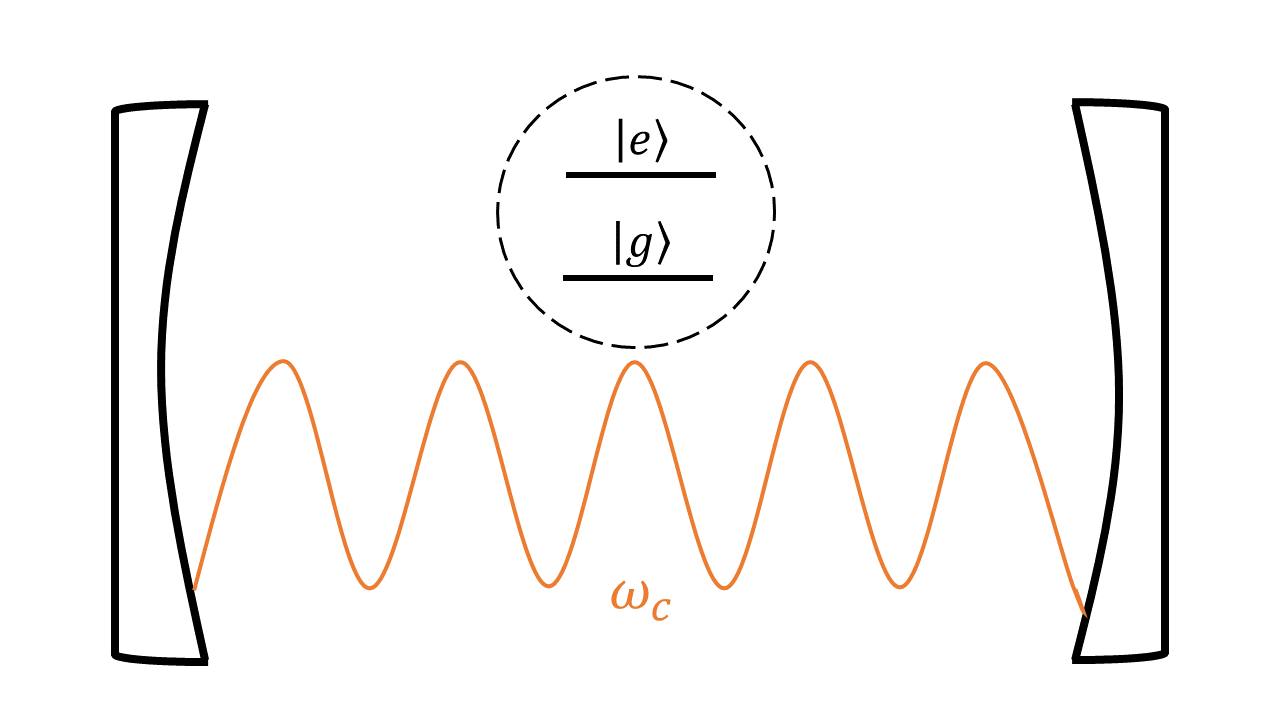
\includegraphics[width=0.65\linewidth]{images/AtomCavity.png}
    \caption{Atom inside the cavity in a quantum regime.}
    \label{fig:atomcavity}
\end{figure}

\subsection{Single-mode cavity}

Consider a cavity with only one mode of the electromagnetic field (\textit{single-mode approximation}) with frequency $\omega_c$ and an atom with only two energy levels; the motion of its center of mass motion can be ignored. The system is presented in figure (\ref{fig:atomcavity}) and the Hamiltonian of this system is made of 
\begin{align*}
    H_\text{light} & = H_{EM} = \hbar \omega_c \crt{} \dsr{} \\
    H_\text{atom} & = H_A = \hbar \omega_{eg} \ket{e}\bra{e} \\
    H_\text{atom-light} & = H_{AL}= -\hat{\Vec{d}} \cdot \hat{\Vec{E}}\\
\end{align*}
Using the expression (\ref{eq:efFP}) for the electric field obtained for a Fabry-Perot cavity for a single mode with frequency $\omega_c = c k_c $ 
\begin{align*}
    \hat{\Vec{E}} = -i \Vec{\epsilon} \sqrt{\frac{\hbar \omega_c}{\varepsilon_0 V}} \sin{(k_c z)} \left( \hat{a}^\dagger - \hat{a} \right), 
\end{align*}
the contribution of the atom-light interaction becomes 
\begin{align*}
    H_{AL} & = - \left( \Vec{d}_{eg} \ket{e}\bra{g} + \Vec{d}^*_{eg} \ket{g}\bra{e} \right) \cdot \left[-i \Vec{\epsilon} \sqrt{\frac{\hbar \omega_c}{\varepsilon_0 V}} \sin(k_c z) \left(\crt{} -  \dsr{}\right)\right] = \\
    &= i \dfrac{\hbar}{2} (\tilde{g} \sigma_{+} + \tilde{g}^{\ast} \sigma_{-}) \left(\crt{} -  \dsr{}\right)
\end{align*}
where the notation previously introduced is used and 
\begin{equation*}
    \tilde{g} = \frac{2\Vec{d}_{eg}^* \cdot \Vec{\epsilon}}{\hbar} \sqrt{\frac{\hbar \omega_c}{\varepsilon_0 V}}  \sin(k_c z)
\end{equation*}
is called \textit{vacuum Rabi frequency}. \\
The total Hamiltonian becomes
\begin{equation}
    H =  \hbar \omega_c \crt{} \dsr{} + \hbar \omega_{eg} \ket{e}\bra{e} + \frac{i \hbar}{2} (\tilde{g} \sigma_{+} +\tilde{g}^{\ast} \sigma_{-}) \left(\crt{} -  \dsr{}\right).
\end{equation}

Consider a situation near resonance regime ($\omega_c \simeq \omega_{eg}$); we know that it is possible to simplify the problem using the rotating-wave approximation, as seen in the previous section. This approximation leads to the elimination of the terms $\sigma_{+} \crt{}$ and $\sigma_{-} \dsr{}$ in $H_{AL}$. More in detail, one can move to a new frame where the energy is conserved through the transformation
\begin{equation}
    R = \underbrace{\exp{{i \omega_{eg} \ket{e}\bra{e} t}}}_{\text{\footnotesize atom}} \, \underbrace{\exp{i \omega_c t \hat{a}^{\dagger} \hat{a}}}_{\text{\footnotesize cavity}} \equiv  R_A \otimes R_{EM}
\end{equation}
Using equation (\ref{eq:transfH}), the new Hamiltonian for the atom-light interaction is 
\begin{align}
    H'_{AL} = \frac{i \hbar}{2} \Tilde{g} \, R \sigma_{+} \hat{a}^{\dagger} R^{\dagger} - \frac{i \hbar}{2} \Tilde{g} \, R \sigma_{+} \hat{a} R^{\dagger} + \text{h.c.}
    \label{eq:atom-light-new}
\end{align}
The first term gives
\begin{align*}
    R \sigma_{+} \hat{a}^{\dagger} R^{\dagger} &= {R_A \sigma_{+} R_A^{\dagger}} \otimes  R_{EM} \hat{a}^{\dagger} R_{EM}^{\dagger} = \\
    &= e^{i \omega_{eg} t } \sigma_{+} \left[  e^{i \omega_c t \hat{a}^{\dagger} \hat{a}} \hat{a}^{\dagger} e^{-i \omega_c t \hat{a}^{\dagger} \hat{a}} \right] 
\end{align*}
and we recognize
\begin{align*}
     e^{i \omega_c t \hat{a}^{\dagger} \hat{a}} \hat{a}^{\dagger} e^{-i \omega_c t \hat{a}^{\dagger} \hat{a}} \equiv  \hat{a}_H^{\dagger}(t)
\end{align*} 
which is the creation operator in the Heisenberg picture for a free harmonic oscillator. Since one can write 
\begin{align*}
    \hat{a}_H^{\dagger}(t) = \hat{a}_H^{\dagger}(0) \, e^{i \omega_c t}, 
\end{align*}
then
\begin{align}
    R \sigma_{+} \hat{a}^{\dagger} R^{\dagger} = e^{i (\omega_{eg} + \omega_c) t} \sigma_{+} \hat{a}_H^{\dagger}(0)
\end{align}
In the same way, one obtains the second term of Eq. \ref{eq:atom-light-new}
\begin{equation}
    R \sigma_{+} \hat{a} R^{\dagger} = e^{i (\omega_{eg} - \omega_c  ) t} \sigma_{+} \hat{a}_H(0)
\end{equation}
Finally, in the in the rotating frame the new Hamiltonian for the atom-light interaction becomes
\begin{equation*}
    H'_{AL}(t) = \underbrace{\frac{i \hbar}{2} \Tilde{g} {e^{i (\omega_{eg} + \omega_c) t}} \sigma_{+} \hat{a}^{\dagger}}_{V^{AL}(t)} + \underbrace{\frac{i \hbar}{2} \Tilde{g} 
    e^{i (\omega_{eg} - \omega_c  )t} \sigma_{+} \hat{a} }_{H^{AL}_0} ~+~ \text{h.c.} 
\end{equation*}
One can notice that the term $H_0$ is independent of time when $\omega_c \simeq \omega_{eg}$, while the term $V(t)$ goes like $e^{2 i \omega_c t}$. Thus, 
\begin{equation*}
    H'_{AL}(t) = \frac{i \hbar}{2} \left[ \tilde{g} e^{2 i \omega_c t} \sigma_+ \hat{a}^\dagger + \tilde{g} \sigma_{+} \hat{a} + \text{h.c.} \right].  
\end{equation*}
The last step consists of going back to the original frame; this leads to 
\begin{align*}
    H_{AL} = -\frac{i \hbar}{2} \tilde{g} \sigma_+ \hat{a} + \frac{i \hbar}{2} \tilde{g}^* \sigma_- \hat{a}^\dagger, 
\end{align*}
from which one can notice that the terms $\sigma_+ \hat{a}^\dagger$ and $\sigma_- \hat{a}$ do not contribute to the dynamics. 
Finally, the rotating-wave approximation is equivalent to the condition
\begin{align*}
    \abs{\omega_{eg} + \omega_c} \gg \abs{\omega_{eg} - \omega_c}, \tilde{g}
\end{align*}
and the total Hamiltonian, which describes the so-called \textbf{Jaynes-Cummings model}, becomes
\begin{align}
    H = \hbar \omega_c \hat{a}^\dagger \hat{a} + \hbar \omega_{eg} \ket{e}\bra{e} -\frac{i \hbar}{2} \tilde{g} \sigma_+ \hat{a} + \frac{i \hbar}{2} \tilde{g}^* \sigma_- \hat{a}^\dagger. 
\end{align}
\\

An alternative form to the model can be obtained by redefining $\Tilde{g} = g e^{i \phi}$, hence
\begin{equation*}
    -i \Tilde{g} \sigma_{+} \hat{a} = g \sigma_{+} \left(-i e^{i\phi} \hat{a} \right) \equiv {g} \sigma_+ \hat{a}',
\end{equation*}
where a unitary transformation allows to introduce $\hat{a}' = -i e^{i\phi} \hat{a}$ and $\hat{a}'^\dagger = i\hat{a}^\dagger e^{-i \phi}$. This implies that $\hat{a}^\dagger \hat{a} = \hat{a}'^\dagger \hat{a}'$ and hence 
\begin{equation} \label{eq:JCModel}
    H = \hbar \omega_c \hat{a}'^\dagger \hat{a}' + \hbar \omega_{eg} \ket{e}\bra{e} + \frac{g \hbar}{2} ( \sigma_+ \hat{a}' + \sigma_- \hat{a}'^\dagger) \qquad \text{with} \qquad g \in \mathbb{R}. 
\end{equation}
This is the model for an atom interacting with a single-mode, nearly resonant ($\omega_{eg} \simeq \omega_{c}$) cavity mode within the rotating-wave approximation, ignoring any dissipation process such as spontaneous emission or any input or output from the cavity.

\subsection{Multi-mode cavity}

To treat a multi-mode, nearly resonant cavity, it is sufficient to consider: 
\begin{align*}
    \sigma_{+} a_n^{\dagger} \quad & \longrightarrow \quad  e^{i(\omega_{eg} + n \omega_c) t} \sigma_{+} a^{\dagger} \\
    \sigma_{+} a_n \quad & \longrightarrow \quad e^{i(\omega_{eg} - n \omega_c) t} \sigma_{+} a
\end{align*}
In this case only $n=1$ would give some relevant terms, the others would be negligible.


\subsection{Dynamics of the Jaynes-Cummings model}

The next step consists of solving the Jaynes-Cummings model; the physics field studying this kind of systems is called \textit{cavity quantum electro-dynamics}.

In order to study the dynamics of the system, one can start from a basis formed with the eigenstates of 
\begin{equation*}
    H_0 = \hbar \omega_c \hat{a}'^\dagger \hat{a}' + \hbar \omega_{eg} \ket{e}\bra{e}. 
\end{equation*}
They are
\begin{align*}
        \ket{g}_A \otimes \ket{n}_{EM} \equiv \ket{g, n} \qquad \text{and} \qquad \ket{e}_A \otimes \ket{n}_{EM} \equiv \ket{e, n}, 
\end{align*}
where $\ket{n}$ is the $n$-photon state in the cavity. 
Taking the atom ground energy as reference value for the zero, the eigenvalues of the eigenstates are given by: 
\begin{align*}
    \ket{g, n} \quad & \longrightarrow \quad E_n^{(g)} = E_A^g + E_{EM}  = 0 + n \hbar \omega_c = \hbar \omega_c n \\
    \ket{e, n} \quad & \longrightarrow \quad E_n^{(e)} = E_A^e + E_{EM}  = \hbar \omega_{eg} + n \hbar \omega_c = \hbar (\omega_{eg}  + \omega_c n )
\end{align*}
These energy levels are reported in figure \ref{fig:JCeigen}, where the decoupling $\delta \equiv \omega_{eg} - \omega_c$ is introduced. 

\begin{figure}[h]
\centering
    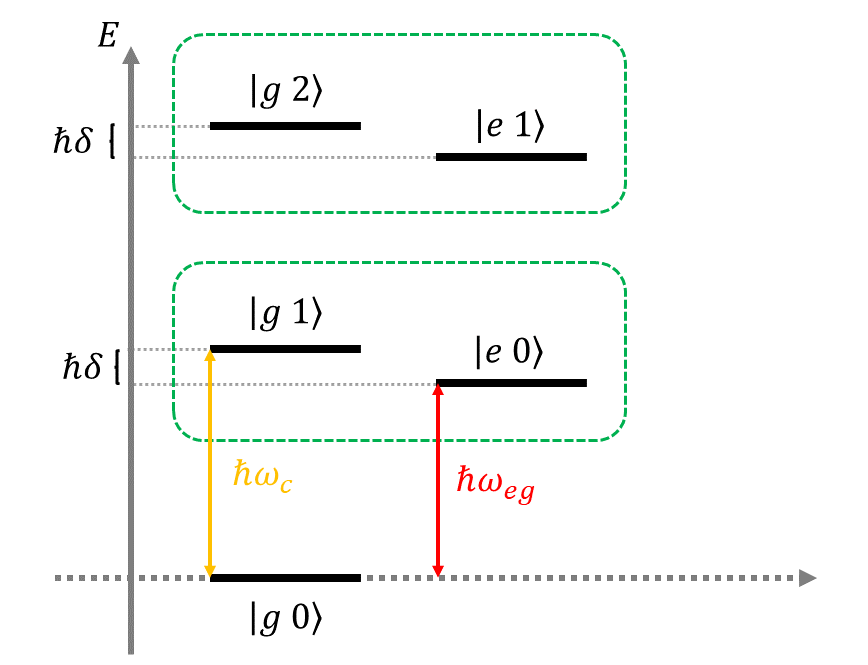
\includegraphics[width=0.57\linewidth]{images/eigenstatesAL.png}
    \caption{Eigenstates of the James-Cummings model (neglecting the atom-light interaction).}
    \label{fig:JCeigen}
\end{figure}

Introducing the interaction between the atom and the cavity, which is described by the last term in Eq. \ref{eq:JCModel}
\begin{equation*}
    H_{AL} = \frac{\hbar g}{2} ({\sigma_{+} \hat{a}} + {\sigma_{-} \hat{a}^{\dagger}}). 
\end{equation*}
the action of this (full) Hamiltonian on the states of the basis is: 
\begin{align*}
    \sigma_+ \hat{a} \ket{g,n} & = \sqrt{n} \ket{e}\bra{g} \ket{g,n-1} = \sqrt{n} \ket{e,n-1}, \\
    \sigma_+ \hat{a} \ket{e,n} & \propto \ket{e}\bra{g} \ket{e,n-1} = 0, \\
    \sigma_- \hat{a}^\dagger \ket{g,n} & \propto \ket{g}\bra{e} \ket{g,n+1} = 0, \\
    \sigma_- \hat{a}^\dagger \ket{e,n} & = \sqrt{n} \ket{g}\bra{e} \ket{e,n+1} = \sqrt{n} \ket{g,n+1}, 
\end{align*}
from which one deduces that $H_{AL}$ only couples 
\begin{align*}
    \ket{g, n} \quad \longleftrightarrow \quad \ket{e,n-1} \qquad \text{and} \qquad 
    \ket{e, n} \quad \longleftrightarrow \quad \ket{g,n+1}. 
\end{align*}
The first relation corresponds to the process of \textit{light absorption}, in which one photon is absorbed by the atom which jumps from the ground state to the excited state, while the second one described the process of \textit{light emission}, in which one photon is emitted from the atom that goes from the excited state to the ground state.

\begin{figure}[t]
\centering
    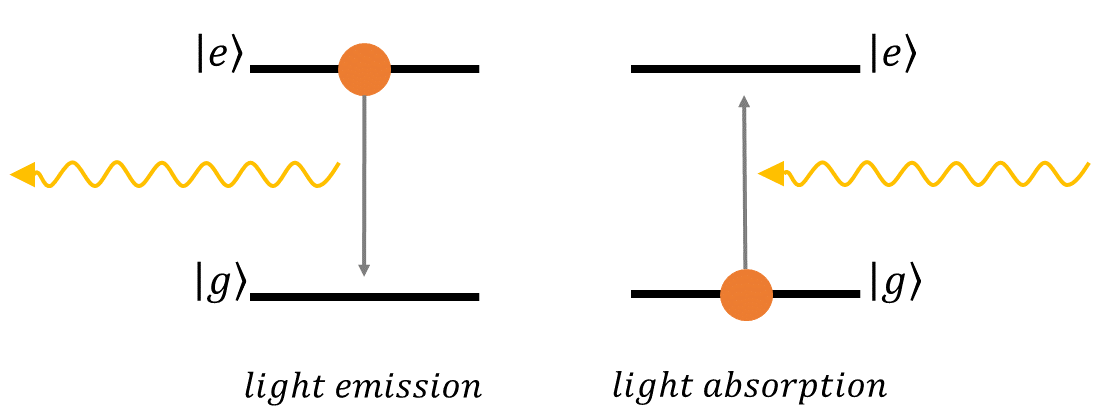
\includegraphics[width=0.67\linewidth]{images/EmsissionAbsorption.png}
    \caption{Processes of light emission and light absorption for an atom with two energy levels: $\ket{g}$ and $\ket{e}$. }
    \label{fig:AbEm}
\end{figure}

The problem ends up being a set of two-levels systems (dotted rectangles in figure \ref{fig:JCeigen}) plus the vacuum state $\ket{g,0}$. Each one of these systems is associated to an Hamiltonian $H_n$ which, in the basis formed by $\ket{g,n}$ and $\ket{e,n-1}$, is given by
\begin{align*}
    H_n & =
    \begin{pmatrix}
    n \hbar \omega_c & \dfrac{g \hbar \sqrt{n}}{2} \\
    \dfrac{\hbar g \sqrt{n}}{2} & \hbar \omega_{eg} +  (n-1) \hbar \omega_c
    \end{pmatrix} = \\ 
        &= n \hbar \omega_c \mathbb{1} + 
        \begin{pmatrix}
            0 & \dfrac{g \hbar \sqrt{n}}{2} \\
            \dfrac{g \hbar \sqrt{n}}{2} & \hbar (\omega_{eg} - \omega_c)
        \end{pmatrix} = \\
        &= n \hbar \omega_c \mathbb{1} +
        \begin{pmatrix} 
            0 & \dfrac{g \hbar \sqrt{n}}{2} \\
            \dfrac{g \hbar \sqrt{n}}{2} & \hbar \delta
        \end{pmatrix}
\end{align*}
Therefore, the total hamiltonian is a $2 \times 2$ block diagonal matrix with the first element of the diagonal being zero (corresponding to $\ket{g, 0}$):
\begin{equation*}
H = \left(
    \begin{array}{ccccc}
     \mathbf{0} &  &  &  \\
     & H_1 &  &  \\
     & & \ddots & \\
     & & & H_n & \\ 
     & & & & \ddots
    \end{array}
\right)
\end{equation*}
As for each $H_n$, one can compute the eigenvalues: 
\begin{equation}
    E_\pm^{(n)} = n \hbar \omega_c + \frac{1}{2} \hbar \delta \pm \frac{\hbar}{2} \sqrt{\delta^2 + g^2 n} \;\;.
    \label{eq:energies}
\end{equation}
This result shows that there is a further separation between $\ket{g, n}$ and $\ket{e, n-1}$, indeed the eigenvectors corresponding to each eigenvalue are 
\begin{align*}
    \ket{+}_n &= \cos \left(\frac{\theta}{2}  \right) \ket{g, n} + \sin\left( \frac{\theta}{2} \right) \ket{e, n-1} \\
    \ket{-}_n &= - \sin\left( \frac{\theta}{2} \right) \ket{g, n} + \cos\left( \frac{\theta}{2} \right) \ket{e, n-1}
\end{align*}
with
\begin{equation*}
    \theta = \arctan \left( \frac{g \sqrt{n}}{\delta}\right).
\end{equation*}
A schematic view of the separation between the eigenstates of the Jaynes-Cumming model is reported in figure \ref{fig:newJCeigen}. 

\begin{figure}[t]
\centering
    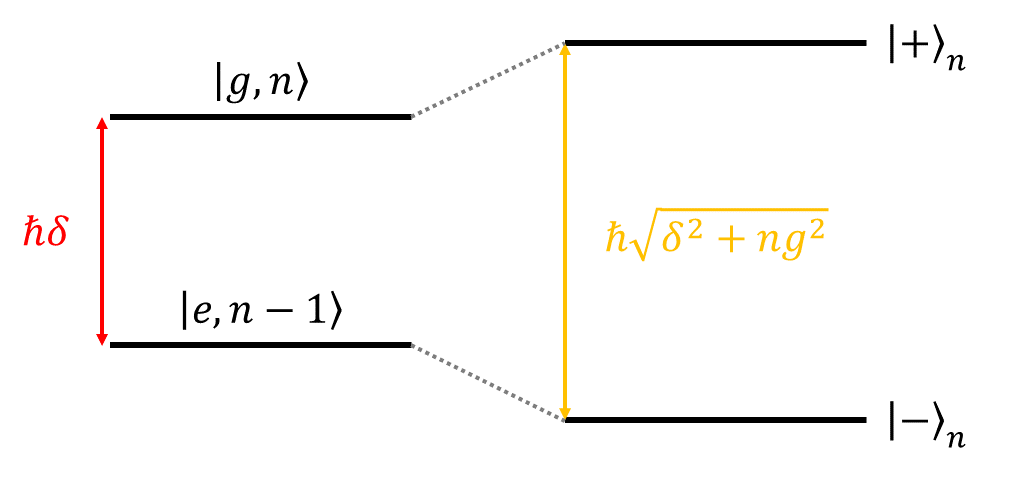
\includegraphics[width=0.6\linewidth]{images/newEigenValue.png}
    \caption{Separation between the eigenstates of the James-Cumming model due to the atom-light interaction.}
    \label{fig:newJCeigen}
\end{figure}

It is important to notice that $\ket{+}_n$ and $\ket{-}_n$ are superpositions of atom and photons modes and they are called \textbf{dressed states}. This superposition is maximum when $\theta = \pi/2$, which is equivalent to the condition $\delta \to 0$ in which $\sin(\theta/2) = \cos{\theta/2}$. When the decoupling is very small, the system is resonant and the separation between eigenvalues, evaluated using (\ref{eq:energies}), becomes $\Delta E_n =  \hbar g \sqrt{n}$. This shows that the Rabi oscillations are now completely quantized since the energy separation between states depends on the number of photons $n$. The separation trend $\omega_n = \Delta E_n$ is reported in figure \ref{fig:omegan}, from which one can notice that the best condition to solve the problem (bigger separation of energies, or lower density) is for low $n$ (far from the classical regime). 

\begin{figure}[h!]
\centering
    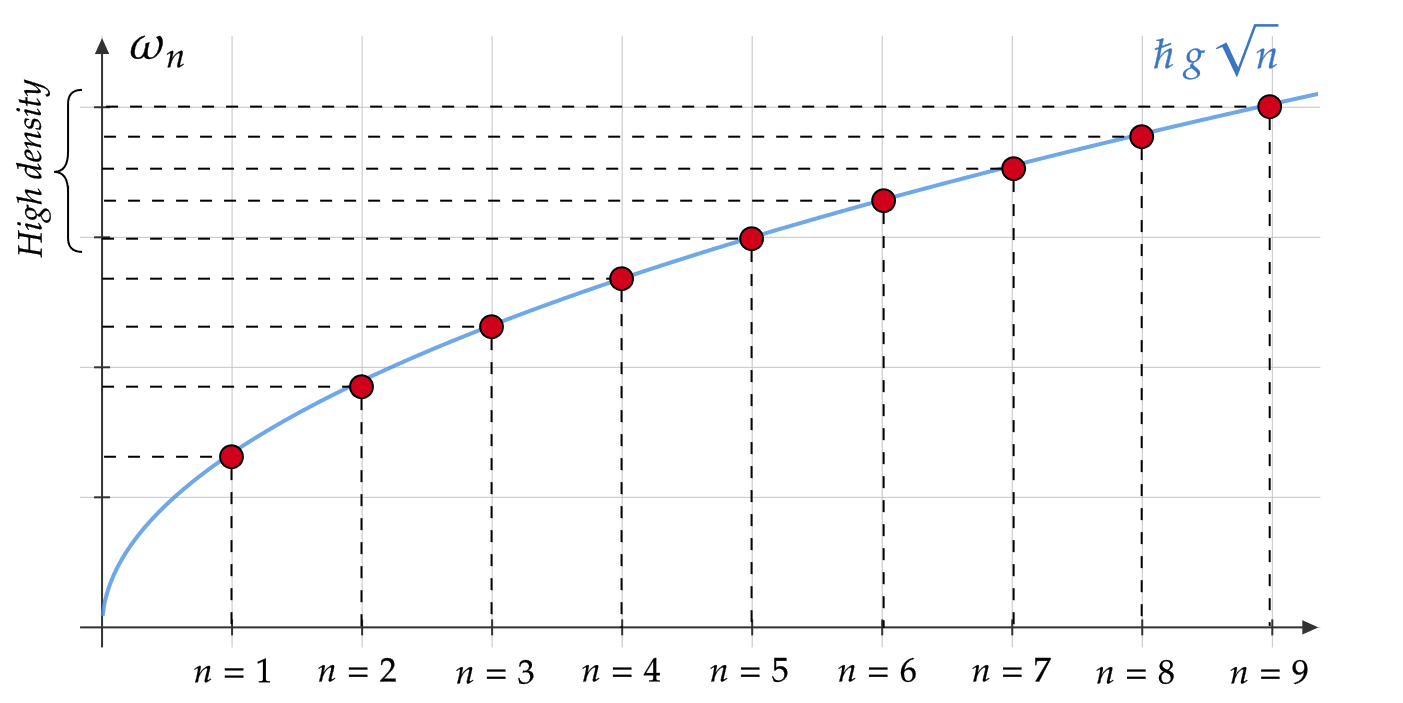
\includegraphics[width=0.8\linewidth]{images/omega_n.png}
    \caption{Frequency associated to the separation of state as a function of the number of photons in the cavity.}
    \label{fig:omegan}
\end{figure}

\subsection{Quantum Rabi oscillations}

Given an initial state $\ket{\psi_0} = \ket{e, n-1} $, it is possible to evaluate the probability that the atom remains in the excited state and the number of photons in conserved (always in the case of a cavity with resonant light, i.e. $\delta \approx 0$): 
\begin{align*}
    P_e^{(n-1)}(t) &\propto \abs{\exp{-iE_+ t/\hbar} + \exp{-iE_- t/\hbar}}^2  \\
    &\propto \abs{\exp{-\frac{i}{2} g \sqrt{n}t } + \exp{\frac{i}{2} g \sqrt{n}t }}^2  \\
    & = \cos^2{\left(\sqrt{n} \, g t\right)}. 
\end{align*}
This trend (shown in Figure \ref{fig:Pe}) represents perfect oscillations, also called \textit{quantum Rabi oscillations}.
% EXPLAIN: only if they are fast compared to the decay time of the system (this happens when the photons exit the cavity). 
\begin{figure}[t]
\centering
    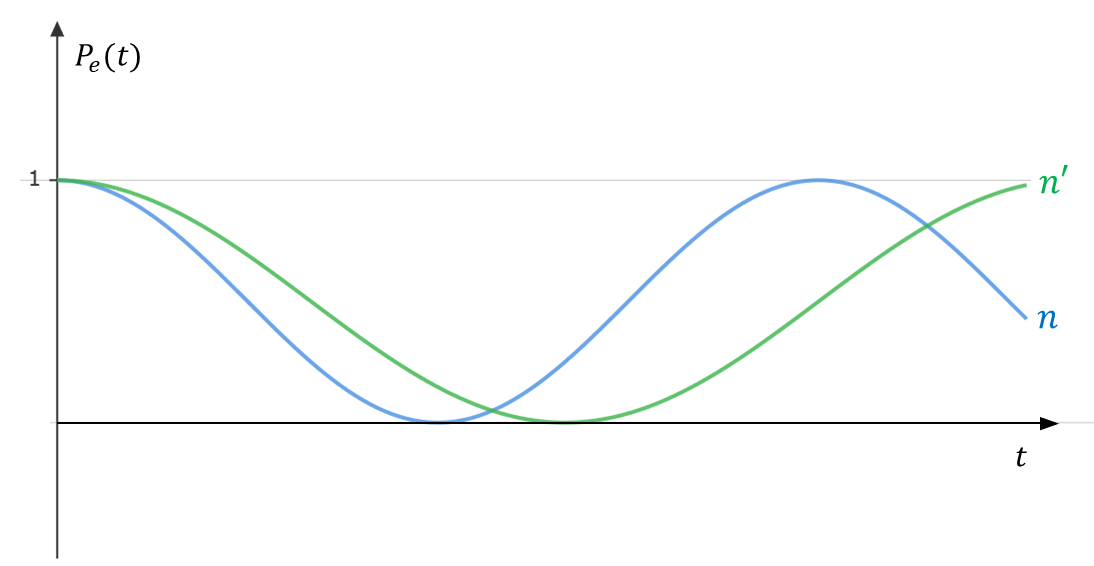
\includegraphics[width=0.7\linewidth]{images/PeJC.png}
    \caption{Probability of finding the atom in the excited state starting from a situation in which the atom is already in the excited state and the number of photons in the cavity are $n$ or $n'$, with $n'<n$. }
    \label{fig:Pe}
\end{figure}

\subsection{Collapses and revivals of the atomic population}

Consider the case in which the initial configuration is $\ket{\psi_0} = \ket{e} \otimes \ket{\alpha}$, with $\ket{\alpha}$ given by equation (\ref{eq:cohstate}), and let $\Bar{n} = \abs{\alpha}^2$. The probability of having an excited state at a time starting from $\psi_0$ is 
\begin{align}
    P_e(t) = |\bra{e}\ket{\psi(t)}|^2 = \sum_{n=1} \abs{c_{n-1}(0)}^2 P_e^{(n-1)}(t), 
    \label{eq:Pe}
\end{align}
where 
\begin{align*}
    \abs{c_{n-1}(0)}^2 = \abs{e^{-\abs{\alpha}^2/2 } \frac{\alpha^{n-1}}{\sqrt{(n-1)!}}}^2 = e^{-\abs{\alpha}^2} \frac{\alpha^{2(n-1)}}{(n-1)!} 
\end{align*} 
indicate the initial occupation probability and $P_e^{(n-1)}$ is similar to the result obtained in the previous section
\begin{align*}
    P_e^{(n-1)} = \cos^2{(\sqrt{\bar{n}+ \delta n} \, gt )}.
\end{align*}
In the last expression, $\delta n$ is introduced to indicate the spread of the distribution which describes the number of photons. Moreover, one can notice that $\delta n/\bar{n} \sim 1/\sqrt{\bar{n}} \to 0$ when $\bar{n} \to \infty$. In this limit, the expression for $P_e^{(n-1)}$ can be rewritten as 
\begin{align*}
    P_e^{(n-1)} & = \cos^2{\left( \sqrt{\bar{n}} gt \sqrt{1 + \frac{\delta n}{\bar{n}}} \right)} \simeq \\
    & \simeq  \cos^2{\left( \sqrt{\bar{n}} gt \left( 1 + \frac{\delta n}{2\bar{n}} \right) \right)} = \\
    & = \cos^2{\left( \sqrt{\bar{n}} gt  + \frac{\delta n}{2\sqrt{\bar{n}}}gt\right)}  = \\
    & = \frac{1}{2} + \frac{1}{2} \cos{\left(2 \sqrt{\bar{n}} g t +  \frac{\delta n}{\sqrt{\bar{n}}}gt \right)} \;\;,
\end{align*}
therefore equation (\ref{eq:Pe}) leads to
\begin{equation*}
    P_e = \frac{1}{2} + \frac{1}{2} \sum_{n=1} \abs{c_{n-1}(0)}^2 \left[ \cos{(2 \sqrt{\bar{n}} gt)} \cos{\left( \frac{\delta n}{\sqrt{\bar{n}}} gt \right)} - \sin{(2 \sqrt{\bar{n}} gt)} \sin{\left( \frac{\delta n}{\sqrt{\bar{n}}} gt \right)}\right]. 
\end{equation*}
Two frequencies are identified from it: 
\begin{align}
    \omega_R \equiv 2 \sqrt{\bar{n}} g \qquad \text{and} \qquad \omega_C \equiv g \frac{\delta n}{\sqrt{\bar{n}}}. 
\end{align}
Having a large average number of photons, one can easily see that $\omega_R \gg \omega_C$ and thus, in the interval $0 < t < (2 \pi)/\omega_C$, only the oscillations with frequency $\omega_R$ are relevant. To better understand what happens, the expression for $P_e(t)$ has to be rewritten in a more convenient form:
\begin{align}
     P_e(t) & = \frac{1}{2} + \frac{1}{2} \sum_{n=0}^\infty e^{-\bar{n}} \frac{\bar{n}^n}{n!} \left[ \cos{\left( 2  \sqrt{\bar{n}} gt + gt \frac{\delta n}{\sqrt{\bar{n}}} \right)}\right] = \label{eq:st1}\\
     &= \frac{1}{2} + \frac{1}{2} \sum_n e^{-\bar{n}} \frac{\bar{n}^n}{n!} \frac{1}{2} \left( \exp{i 2 \sqrt{\bar{n}} gt} \exp{igt\frac{n-\bar{n}}{\sqrt{\bar{n}}}} + \text{c.c.} \right) = \nonumber \\
     & = \frac{1}{2} + \frac{1}{4}\left[ e^{-\bar{n}} \sum_n \left( \frac{\bar{n}^n}{n!} \exp{igt\frac{n}{\sqrt{\bar{n}}}}\right) \exp{i2\sqrt{\bar{n}}gt - igt\frac{\bar{n}}{\sqrt{\bar{n}}}} + \text{c.c.} \right] =  \nonumber\\
     & = \frac{1}{2} + \frac{1}{4} \left[ e^{-\bar{n}} \exp{\bar{n}e^{igt/\sqrt{\bar{n}}}} e^{i \sqrt{\bar{n}}gt} + \text{c.c.} \right] \equalexpl{we develop the exponent of exponent}  \nonumber\\
     & \simeq \frac{1}{2} + \frac{1}{4} \left[ e^{-\bar{n}} \cdot e^{\bar{n}} \, e^{i\sqrt{\bar{n}}gt} \, e^{-g^2 t^2/2} \cdot e^{i\sqrt{\bar{n}}gt} \,  + \text{c.c.} \right] =  \nonumber\\
    &= \frac{1}{2} + \frac{1}{4} \left[ e^{2i\sqrt{\bar{n}}gt} e^{-\frac{1}{2} g^2 t^2} + \text{c.c.} \right] = \nonumber \\
     & = \frac{1}{2} + \frac{1}{2} \cos{\left(2 \sqrt{\bar{n}}gt\right)} e^{-\frac{1}{2}g^2 t^2} \label{eq:stfin}
\end{align}
The cosine term represents the oscillations with frequency $\omega_R$, while the exponential coefficient corresponds to a damping with \textit{collapse time} $\tau_C \sim \sqrt{2}/g$. It is important to underline that the last term does not correspond properly to a damping, but it is better to consider it as a dephasing, since it has been obtained summing over all the possible frequencies. 

\begin{center}
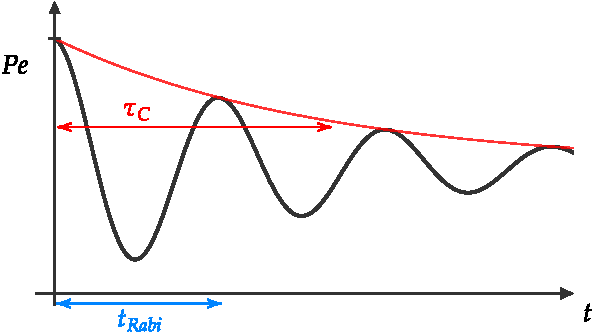
\includegraphics[scale=0.6]{img/Rabi_scales_2.pdf}
\end{center}

From the previous analysis, two time scales have been identified: the one associated to the Rabi frequency ($t_\text{Rabi}$) and the one of the exponential damping ($\tau_C$). In addition to that, there is another time scale that must be considered, which is obtained taking times such that 
\begin{align}
    \frac{gt}{\sqrt{\bar{n}}} = 2 \pi m \qquad \text{with} \qquad m \in \mathbb{N}. 
    \label{eq:revival}
\end{align}
Inserting this value in (\ref{eq:st1}), one obtains $P_e \sim \cos{(4 \pi m\bar{n} + 2 \pi m \delta n)} \sim 1$, and hence the probability reaches again its maximum value every $t$ which satisfies (\ref{eq:revival}), i.e after the so-called \textit{revival time}. An example of the full dynamics is reported in the following figure. 

\begin{center}
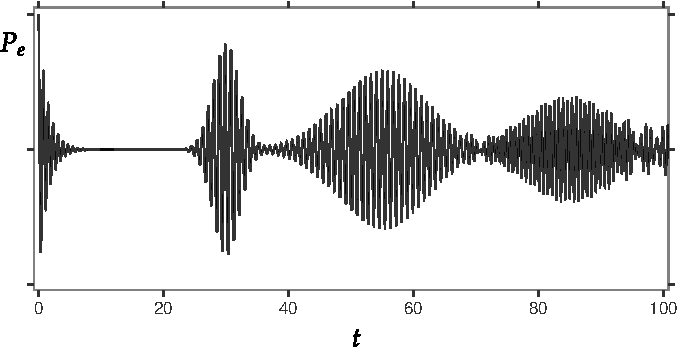
\includegraphics[scale=0.7]{img/Rabi_scales_1.pdf}
\end{center}


\section{Two-level atom coupled with a bath}

Consider a two-level atom coupled with a bath in which many modes are available. This means that, if the atom is in the excited state, there are several decay channels in the bath. The Hamiltonian for this system is made of $H_A$, $H_{EM}$ and $H_{AL}$ which can be written in the rotating-wave approximation
\begin{align}
    H_{AL} = -\vec{d}_{eg} \sigma_+ \hat{\vec{E}}^{(+)} - \vec{d}_{eg}^* \sigma_- \hat{\vec{E}}^{(-)}
\end{align}
with
\begin{align}
    \hat{\vec{E}}^{(+)} &= -i \sum_{\vec{k}, \lambda} \sqrt{\frac{\hbar \omega_k}{2 \varepsilon_0 V}} \vec{\epsilon}_\lambda \,\hat{a}_{\vec{k},\lambda}, \\
    \hat{\vec{E}}^{(-)} &= i \sum_{\vec{k}, \lambda} \sqrt{\frac{\hbar \omega_k}{2 \varepsilon_0 V}} \vec{\epsilon}_\lambda \,  \hat{a}_{\vec{k},\lambda}^\dagger.
\end{align}
These terms correspond to the excitation and de-excitation of the atom after the interaction with light.
This problem can be solved using the Lindblad Master Equation (\ref{eq:cos}) (also called \textit{Nakajima-Zwanzig Equation}) presented in section \ref{sec:ME} and considering
\begin{align*}
    {S'}_\alpha(t') \equiv \sigma_+(t') \qquad  \text{and} \qquad {S'}_\beta^\dagger(t) \equiv \sigma_-(t)
\end{align*}
\begin{align*}
    \hat{B}_\alpha \equiv  i \vec{d}_{eg}^* \cdot \hat{\vec{E}}^{(-)}  \qquad \text{and} \qquad \hat{B}_\beta^\dagger \equiv - i \vec{d}_{eg} \cdot \hat{\vec{E}}^{(+)}. 
\end{align*}
Moreover, 
\begin{align*}
    \sigma_-(t') = \sigma_-(0) \, e^{-i \omega_{eg} t'} \qquad \text{and} \qquad \sigma_+(t) = \sigma_+(0) \, e^{i \omega_{eg} t}. 
\end{align*}
Therefore, the first term of equation (\ref{eq:cos}) becomes
\begin{align*}
    & \int_0^t dt'\, G_{\alpha\beta}(t-t')  \sigma_-(0)  e^{-i \omega_{eg} t'} {\rho'}_S(t') \sigma_+(0)  e^{i \omega_{eg} t} = \\
    & = \int_0^t dt'\,  G_{\alpha\beta}(t-t') e^{i \omega_{eg}(t-t')} \sigma_-(0) \rho'_S(t') \sigma_+(0);
\end{align*}
introducing the variable $\tau \equiv t-t'$ and assuming that $\rho(\tau)$ is smoothly evolving over the time scale at which $G_{\alpha \beta}(\tau)$ decays ($\rho'_S(t-\tau) \simeq \rho'_S(t)$), it can be written as 
\begin{align*}
    - \left[\int_t^0 d\tau \, G_{\alpha \beta}(\tau) e^{i \omega_{eg}\tau} \right]\sigma_- \rho'_S(t) \sigma_+. 
\end{align*}
For the same reason, the lower limit of this integral can be taken $t\to\infty$. Therefore, all the terms in the Master Equation in this assumption has an integral coefficient with the generic form
\begin{align*}
    \mathcal{G}(\omega_{eg}) \equiv \int_0^\infty d \tau \, G_{--}(\tau) e^{i \omega_{eg} \tau} \qquad \text{with} \qquad G_{--}(\tau) = \langle \left( \vec{d}_{eg} \cdot \hat{\vec{E}}^{(+)}(\tau) \right) \left( \vec{d}_{eg}^* \cdot \hat{\vec{E}}^{(-)}(0)\right)  \rangle_B  
\end{align*}
An element of this expectation value can be written as 
\begin{align*}
    \langle \hat{a}_{\vec{k},\lambda}(\tau) \hat{a}^\dagger_{\vec{k}',\lambda'}(0)\rangle_B &= \langle e^{-i \omega_k t} \hat{a}_{\vec{k},\lambda}(0) \hat{a}^\dagger_{\vec{k}',\lambda'}(0)\rangle_B = \\ &= \langle \hat{a}_{\vec{k},\lambda}(0) \hat{a}^\dagger_{\vec{k}',\lambda'}(0)\rangle_B = \\
    & = \delta_{\vec{k},\vec{k}'} \delta_{\lambda,\lambda'} \left(\mathbb{1}-\langle \hat{a}^\dagger_{\vec{k}',\lambda'} \hat{a}_{\vec{k},\lambda}(0)\rangle_B\right). 
\end{align*}
The term $\langle \hat{a}^\dagger_{\vec{k}',\lambda'}\hat{a}_{\vec{k},\lambda}(0)\rangle_B$ can be ignored since it corresponds to the average number of background photons in the bath (like the CMB = cosmic microwave background). Therefore, 
\begin{align}
    \langle \hat{a}_{\vec{k},\lambda}(\tau) \hat{a}^\dagger_{\vec{k}',\lambda'}(0)\rangle_B \simeq \delta_{\vec{k},\vec{k}'} \delta_{\lambda,\lambda'}
\end{align}
and 
\begin{align*}
    \qquad G_{--}(\tau) = \frac{\hbar \omega_k}{2 \varepsilon_0 V} \sum_{\vec{k},\lambda} e^{-i\omega_k t} \left( \vec{d}_{eg} \cdot \vec{\epsilon}_\lambda \right)\left( \vec{d}_{eg}^* \cdot \vec{\epsilon}_\lambda \right). 
\end{align*}
Using the continuum limit to rewrite the summation over $\vec{k}$ and considering the projections of $\vec{d}_{eg}$ and $\vec{d}_{eg}^*$ on $\vec{\epsilon}_1$ and $\vec{\epsilon}_2$, one as 
\begin{align*}
    \qquad G_{--}(\tau) &= \frac{\hbar \omega_k}{2 \varepsilon_0 V} \frac{1}{(2\pi)^2} \int d^3 \vec{k} \, e^{-i\omega_k t} \sum_\lambda \abs{({d}_{eg})_\lambda}^2 = \\
    & = \frac{\hbar \omega_k}{2 \varepsilon_0 V} \frac{1}{(2\pi)^2} \int d^3 \vec{k} \, e^{-i\omega_k t}  \abs{\vec{d}_{eg}}^2 \sin^2{\theta}, 
\end{align*}
where $\theta$ is the angle between $\vec{d}_{eg}$ and the plane of $\vec{\epsilon}_1$ and $\vec{\epsilon}_2$. From this result, the spherical coordinates (with the solid angle $d \Omega$) can be used to rewrite the integral over $d^3 \vec{k}$ and the complete expression is 
\begin{align*}
    \mathcal{G}(\omega_{eg}) 
    &= \int_0^\infty d \tau \, \int \frac{d \Omega}{(2 \pi)^3} \sin^2 \theta \int_0^\infty dk \, k^2 \frac{\hbar \omega}{2 \varepsilon_0} e^{-i(\omega-\omega_{eg})\tau} |{\vec{d}_{eg}}|^2 = \\
    &= \frac{\hbar c |{\vec{d}_{eg}}|^2 }{2 \varepsilon_0 (2\pi)^3} \int d\Omega \, \sin^2 \theta \int_0^\infty dk \, k^3 \int_0^\infty d \tau \, e^{-i(\omega-\omega_{eg})\tau} = \\
    &= \frac{2 \hbar |{\vec{d}_{eg}}|^2  }{3 \varepsilon_0 (2 \pi)^3 c^3} \int_0^\infty d\omega \, \omega^3 \int_0^\infty d\tau \, e^{-i(\omega-\omega_{eg})\tau}, 
\end{align*}
where the relation $\omega_k \equiv \omega = c k$ is used. The last integral is quite tricky. In the following, we will consider its real and imaginary parts.\\
To write the complete Master Equation, the other correlators (similar to $G_{\alpha \beta}$) should be taken into account; it is possible to prove that they are all null. Hence the final expression is 
\begin{align*}
    \dot{\rho}'_S(t) &= \frac{1}{\hbar^2} \bigg\{ \real( \mathcal{G}(\omega_{eg})) \left( \sigma_-\rho_S \sigma_+ - \sigma_+ \sigma_- \rho_S \right) ~+ \\
    &~~+ \real( \mathcal{G}(\omega_{eg})) \left( \sigma_- \rho_S \sigma_+ - \rho_S \sigma_+ \sigma_- \right) ~+ \\
    &~~+i \mathfrak{I}(\mathcal{G}(\omega_{eg})) (\rho_S \sigma_+ \sigma_- - \sigma_+ \sigma_- \rho)\bigg\}. 
\end{align*}
The final step consists of going back to the Schr\"odinger picture to write 
\begin{equation}
    \begin{split}
        \dot{\rho_S} &= \frac{i}{\hbar} \left[ \rho_S,H_S \right] + \frac{i}{\hbar} \mathfrak{I} (\mathcal{G}(\omega_{eg})) \left[ \rho_S, \sigma_+ \sigma_-\right]~+ \\ 
        &~~+ \frac{i}{\hbar^2} \real(\mathcal{G}(\omega_{eg})) \left( \sigma_- \rho_S \sigma_+ - \bigg\{ \sigma_+ \sigma_-, \rho_S \bigg\}\right) 
    \end{split}
\end{equation}

\noindent Two final observations can be done: 
\begin{itemize}
    \item Since $\sigma_+ \sigma_- = \ket{e}\bra{e}$, one can introduce a re-normalized Hamiltonian 
\begin{align*}
    \bar{H}_S = \ket{e}\bra{e} \left( \hbar \omega_{eg} + \frac{1}{\hbar} \mathfrak{I}(\mathcal{G}(\omega_{eg})) \right). 
\end{align*}
The last term is divergent and this problem can be fixed considering the relativistic contributions to the Hamiltonian (in QED different techniques are used to solve it). If this is done, tha imaginary part is just a constant energy shift, called \textit{Lamb shift}. 
\item Introducing 
\begin{equation}
    \Gamma_{eg} \equiv \frac{2}{\hbar^2} \real (\mathcal{G}(\omega_{eg}) =  \frac{|\vec{d}_{eg}|^2 \omega^3_{eg}}{3 \pi \varepsilon_0 \hbar c^3}
\end{equation}
\end{itemize}
one can define the \textit{inverse lifetime} of the excited state 
\begin{align}
    \Gamma_e \equiv{\sum_g} \Gamma_{eg} 
\end{align}













\section{Two-level atom in a dissipative system}

Consider a two-level atom, a source of coherent light and a dissipation described by the quantity $\Gamma$. As seen, in the rotating frame with $\omega \gg \delta, \Omega$, the Hamiltonian is given by equation (\ref{eq:Hrw}), while the Lindblad Master Equation is
\begin{equation}
    \frac{\partial}{\partial t} {\rho} = \frac{i}{\hbar} [\rho,H] + \frac{\Gamma}{2} [2 \sigma_- \rho \sigma_+ - \sigma_+ \sigma_- \rho - \rho \sigma_+ \sigma_-]. 
\end{equation}
The latter can be used to study the evolution of $\langle \sigma_-\rangle$ and $\langle \sigma_+\rangle$, starting from 
\begin{align*}
    \frac{\partial}{\partial t} \langle \sigma_-\rangle = \frac{\partial}{\partial t} \text{Tr}[\rho \sigma_-] = \text{Tr}\left[\frac{\partial}{\partial t} {\rho} \sigma_-\right] 
\end{align*}
and inserting it in the Master Equation 
\begin{align*}
    \frac{\partial}{\partial t} \langle \sigma_-\rangle &= \text{Tr} \left\{ \left[ \frac{i}{\hbar} (\rho H - H \rho) + \frac{\Gamma}{2} \left( 2 \sigma_- \rho \sigma_+ - \sigma_+ \sigma_- \rho - \rho \sigma_+ \sigma_-\right)\right] \sigma_- \right\} = \\
    & = \frac{i}{\hbar} \text{Tr} \left[ \rho \left(\hbar \delta \ket{e}\bra{e} + \frac{\hbar \Omega}{2} \sigma_+ + \frac{\hbar \Omega}{2} \sigma_- \right) \sigma_- \right] + \\
    &~~~ -\frac{i}{\hbar} \text{Tr} \left[ \left(\hbar \delta \ket{e}\bra{e} + \frac{\hbar \Omega}{2} \sigma_+ + \frac{\hbar \Omega}{2} \sigma_- \right) \rho \sigma_- \right] + \\
    & ~~~ +\frac{\Gamma}{2} \text{Tr} \left[ 2 \sigma_- \rho \sigma_+ \sigma_- - \sigma_+ \sigma_- \rho  \sigma_- - \rho \sigma_+ \sigma_- \sigma_- \right] = \\
    &= \frac{i}{\hbar} \text{Tr}\left[ \frac{\hbar \Omega}{2} \rho \sigma_+ \sigma_-\right] - \frac{i}{\hbar} \text{Tr}\left[ \hbar \delta \underbrace{\ket{e}\bra{e} \rho \sigma_-}_{\rho \sigma_-} \right] - \frac{i}{\hbar} \text{Tr}\left[ \frac{\hbar \Omega}{2}  \sigma_+  \rho\sigma_-\right] + \\
    & ~~~ +\frac{\Gamma}{2} \text{Tr} \left[ \underbrace{\ket{e}\bra{e} \rho \sigma_-}_{\rho \sigma_-}\right] = \\
    & = \frac{i}{\hbar} \frac{\hbar \Omega}{2} \text{Tr}[\rho \ket{e}\bra{e}] - \frac{i}{\hbar} \hbar \delta \, \text{Tr}[\rho \sigma_-] - \frac{i}{\hbar} \frac{\hbar \Omega}{2} \text{Tr} \left[ \ket{g}\bra{g} \rho \right] - \frac{\Gamma}{2} \text{Tr} \left[ \rho \sigma_- \right] = \\
    &= i \frac{\Omega}{2} \text{Tr} [\rho \sigma^z] - i \delta \, \text{Tr} [\rho \sigma_-] - \frac{\Gamma}{2} \text{Tr} [\rho \sigma_-] = \\
    &= i\frac{\Omega}{2} \langle \sigma^z \rangle - \left(i \delta +\frac{\Gamma}{2} \right)  \langle \sigma_- \rangle .
\end{align*}
The evolution equation for $\langle \sigma_+ \rangle$ is obtained from the complex conjugate of this result, while a similar procedure leads to the evolution equation for $\langle \sigma^z \rangle$. These equations can be put in matrix form: 
\begin{equation}
    \frac{\partial}{\partial t}
    \begin{pmatrix}
        \langle \sigma_- \rangle \\ \langle \sigma_+ \rangle \\ \langle \sigma^z \rangle
    \end{pmatrix} = 
    \begin{pmatrix}
        -i\delta -{\Gamma}{2} & 0 & {i\Omega}/{2} \\
        0 & i\delta -{\Gamma}/{2} & -{i\Omega^*}/{2} \\
        i \Omega^* & -i \Omega & -\Gamma 
    \end{pmatrix}
    \begin{pmatrix}
        \langle \sigma_- \rangle \\ \langle \sigma_+ \rangle \\ \langle \sigma^z \rangle
    \end{pmatrix} - \begin{pmatrix}
        0 \\ 0 \\ \Gamma
    \end{pmatrix}
\end{equation}
or equivalently 
\begin{align}
    \frac{\partial}{\partial t} \vec{S} = M \vec{S} - \vec{R}. 
\end{align}
These equations are called \textbf{Optical Bloch Equations}.

\subsection{Stationary states of the Optical Bloch Equations}

Non trivial stationary states are given by 
\begin{align*}
    \vec{S}_\infty = M^{-1} \vec{R}, 
\end{align*}
from which 
\begin{align*}
    \langle \sigma_- \rangle_\infty & = -\frac{\Omega (2 \delta + i \Gamma)}{\Gamma^2 + 4 \delta^2 + 2 \abs{\Omega}^2} \\
     \langle \sigma_+ \rangle_\infty & = -\frac{\Omega (2 \delta - i \Gamma)}{\Gamma^2 + 4 \delta^2 + 2 \abs{\Omega}^2} \\
      \langle \sigma^z \rangle_\infty & = -\frac{\Gamma^2 + 4 \delta^2}{\Gamma^2 + 4 \delta^2 + 2 \abs{\Omega}^2}. 
\end{align*}
One can also introduce the \textit{saturation parameter}
\begin{align}
    \mathcal{S} \equiv \frac{2\dfrac{\abs{\Omega}^2}{\Gamma^2}}{1+\dfrac{4\delta^2}{\Gamma^2}}, 
\end{align}
which allows to rewrite the previous results as 
\begin{align}
    \abs{\langle \sigma_- \rangle_\infty }^2 = \frac{\mathcal{S}}{2(1+\mathcal{S})^2} \qquad \text{and} \qquad \langle \sigma^z \rangle_\infty = \frac{1}{1+\mathcal{S}} 
\end{align}
\\

\noindent In addition to that, one can evaluate the probability of being in an excited state
\begin{align*}
    P_e = \rho_{ee} = \text{Tr}[\rho \ket{e}\bra{e}] = \text{Tr}\left[ \rho \left( \frac{\mathbb{1}}{2} + \frac{\sigma^z}{2} \right)\right] = \frac{1}{2} \text{Tr}[\rho] + \frac{1}{2} \langle \sigma^z \rangle = \frac{1}{2} \langle \sigma^z \rangle
\end{align*}
and, using the results for the stationary states, 
\begin{align*}
    P_e^\infty = \lim_{t\to \infty} P_e = \frac{1}{2}\langle \sigma^z \rangle_\infty =  \frac{1}{2(1+\mathcal{S})} =\frac{\Omega^2}{2\Omega^2 + 4 \delta^2 + \Gamma^2}. 
\end{align*}

\begin{center}
\scalebox{1.4}{ 

\tikzset{every picture/.style={line width=0.75pt}} %set default line width to 0.75pt        

\begin{tikzpicture}[x=0.75pt,y=0.75pt,yscale=-1,xscale=1]
%uncomment if require: \path (0,122); %set diagram left start at 0, and has height of 122

%Curve Lines [id:da8052966326082212] 
\draw [line width=0.75]    (46.93,79.33) .. controls (69.93,69.33) and (90.17,44.83) .. (105.17,44.83) .. controls (120.17,44.83) and (142.43,70.33) .. (166.43,78.33) ;
%Straight Lines [id:da4526791024224187] 
\draw    (105.28,113.33) -- (105.28,17.33) ;
\draw [shift={(105.28,15.33)}, rotate = 90] [color={rgb, 255:red, 0; green, 0; blue, 0 }  ][line width=0.75]    (6.56,-1.97) .. controls (4.17,-0.84) and (1.99,-0.18) .. (0,0) .. controls (1.99,0.18) and (4.17,0.84) .. (6.56,1.97)   ;
%Straight Lines [id:da06360510795593066] 
\draw    (10.5,105.6) -- (199.43,105.6) ;
\draw [shift={(201.43,105.6)}, rotate = 180] [color={rgb, 255:red, 0; green, 0; blue, 0 }  ][line width=0.75]    (6.56,-1.97) .. controls (4.17,-0.84) and (1.99,-0.18) .. (0,0) .. controls (1.99,0.18) and (4.17,0.84) .. (6.56,1.97)   ;
%Straight Lines [id:da559598823855056] 
\draw    (103,32.5) -- (107.93,32.5) ;
%Curve Lines [id:da04885805308328728] 
\draw [line width=0.75]    (55.93,100.83) .. controls (94.93,87.83) and (90.43,52.33) .. (105.43,52.33) .. controls (120.43,52.33) and (114.93,88.22) .. (154.43,100.72) ;

% Text Node
\draw (203,96.4) node [anchor=north west][inner sep=0.75pt]  [font=\scriptsize]  {$\delta /\Gamma $};
% Text Node
\draw (109.5,29.4) node [anchor=north west][inner sep=0.75pt]  [font=\tiny]  {$1/2$};
% Text Node
\draw (20,57.4) node [anchor=north west][inner sep=0.75pt]  [font=\scriptsize]  {$\Omega \gg \Gamma $};
% Text Node
\draw (20,88.4) node [anchor=north west][inner sep=0.75pt]  [font=\scriptsize]  {$\Omega \ll \Gamma $};
% Text Node
\draw (110.5,7.2) node [anchor=north west][inner sep=0.75pt]  [font=\scriptsize]  {$P_{e}$};

\end{tikzpicture}
 }
\end{center}


\noindent From this expression, we recognize that two regimes are possible: 
\begin{itemize}
    \item weak drive: 
    \begin{align*}
        \Omega \ll \Gamma \qquad \implies \qquad P_e \simeq \frac{\Omega^2}{4 \delta^2 + \Gamma^2}, 
    \end{align*} 
    which is Lorentzian with width $\sim \Gamma$; 
    \item strong drive: 
    \begin{align*}
        \Omega \gg \Gamma \qquad \implies \qquad P_e \simeq \frac{\Omega^2}{4 \delta^2 + 2\Omega^2}, 
    \end{align*} 
    which is Lorentzian with width $\sim \Omega$; 
\end{itemize}

\section{Three-level atoms and Raman coupling}

Consider a three-level atom, with two quasi-ground states (meaning that they are very stable) $\ket{g_i}, i = 0,1\;$, and a short-lived excited state $\ket{e}$; assume that transitions between the quasi-ground states are forbidden. A schematic view is reported in figure \ref{fig:lambda}. 
\begin{figure}[h]
\centering
    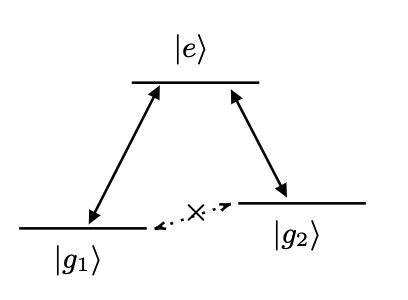
\includegraphics[width=0.3\linewidth]{images/lambda_system.png}
    \caption{$\Lambda$ system with suppressed transition between the ground states. }
    \label{fig:lambda}
\end{figure}

The Hamiltonian for the atom and for the atom-light interaction are 
\begin{align*}
H_{A} &= -\hbar \omega_{g_1} \ket{g_1}\bra{g_1} -\hbar \omega_{g_2} \ket{g_2}\bra{g_2} + 0\\
H_{AL} &= - \hat{\vec{d}} \cdot \hat{\vec{E}},
\end{align*}
where the dipole transition term evaluates as
\begin{equation*}
\begin{aligned}
{\vec{d}} = -e{\vec{r}}  ~\big\rvert_{g_1,g_2,e} & =  -e\ket{g_1}\bra{g_1}\vec{r}\ket{e}\bra{e} \;\;- e\ket{g_2}\bra{g_2}\vec{r}\ket{e}\bra{e} \;\; + \text{h.c.} \\
&\equiv d_{eg_1}^*\ket{g_1}\bra{e} \;\;+\;\; d_{eg_2}^*\ket{g_2}\bra{e} \;\; + \text{h.c}.
\end{aligned}
\end{equation*}
In this derivation, we will write the electric field is written in a slightly different way with respect to the previous chapters: 
\begin{equation*}
\vec{E} =
\sum_{\vec{k},\lambda} \sqrt{\frac{\hbar\omega_k}{2\varepsilon_0}}\vec\epsilon_{\lambda} \, 2 \mathfrak{Im} \left[u_{\vec{k},\lambda}(\vec{r}_\text{atom})\hat{a}_{\vec{k},\lambda}\right], 
\end{equation*}
since for a generic operator $A$ one can write $\mathfrak{Im} A = (A-A^\dagger)/2i$. Notice that $\vec{r}_\text{atom}$ is evaluated in center-of-mass coordinate and not in the coordinates of the electron. 

Consider two independent lasers to control the system
\begin{equation*}
\ket{\psi_\text{lasers}} = \ket{0} \otimes \dots \otimes \ket{0} \otimes \underbrace{\ket{\alpha_1}}_{\substack{\textrm{first laser}\\k_1,\lambda_1}} \otimes \ket{0} \otimes \dots \otimes \ket{0} \otimes \underbrace{\ket{\alpha_2}}_{\substack{\textrm{second laser}\\k_2,\lambda_2}} \otimes \ket{0} \otimes \dots,
\end{equation*}
and assume that: 
\begin{itemize}
    \item $\vec{E}$ is perceived by the system as an averaged value
    \begin{align*}
    \bra{\psi_\text{lasers}}\vec{E}\ket{\psi_\text{lasers}} & = \sqrt{\frac{\hbar\omega_1}{2 \varepsilon_0}}
\vec\epsilon_{\lambda_1} 2 \mathfrak{Im} \left(u_{\vec{k}_1,\lambda_1}\right) \bra{\alpha_1}\hat{a}_{\vec{k}_1,\lambda_1} \ket{\alpha_1} + \left(\substack{\text{same for}\\\vec{k}_2, \lambda_2 }\right)\\ 
& = \sqrt{\frac{2\hbar\omega_1}{\varepsilon_0}}
\vec\epsilon_{\lambda_1} |u_{\vec{k}_1,\lambda_1}||\alpha_1| \cos\left[(c k_1)t + \phi_1\right] + \left(\substack{\text{same for}\\\vec{k}_2, \lambda_2 }\right),
    \end{align*}
    \item the lasers are powerful and hence the state $\ket{\psi}_\text{laser}$ is not much affected by the absorption of one photon.
\end{itemize}
The average value of the electric field can be rewritten as  
    \begin{align}
        \langle \vec{E}\rangle =
\vec{\mathcal{E}}_1 \cos\left(\omega_1t + \phi_1\right) +
\vec{\mathcal{E}}_2 \cos\left(\omega_2t + \phi_2\right). 
    \end{align}
From the previous considerations
\begin{align*}
    H_{AL} & = - \hat{\vec{d}} \cdot \langle \vec{E}\rangle = \\
    &= -\left(
    \vec{d}_{eg_1}\ket{e}\bra{g_1} \;+\; 
    \vec{d}_{eg_2}\ket{e}\bra{g_2} \;+\; 
    \vec{d}_{eg_1}^*\ket{g_1}\bra{e} \;+\; 
    \vec{d}_{eg_2}^*\ket{g_2}\bra{e}
\right)
\cdot\\
&\qquad \cdot\left(
    \vec{\mathcal{E}}_1 \cos\left(\omega_1t + \phi_1\right)
    \;+\;
    \vec{\mathcal{E}}_2 \cos\left(\omega_2t + \phi_2\right)
\right). 
\end{align*}
A formal simplification can be done by introducing the the coefficients
\begin{equation*}
      \Omega_1 = \frac{\vec{d}_{eg_1} \cdot \vec{\mathcal{E}}_1}{\hbar}
      \qquad\qquad
      \Omega_2 = \frac{\vec{d}_{eg_2} \cdot \vec{\mathcal{E}}_1}{\hbar}
\end{equation*}
\begin{equation*}
    \cancel{\Omega}_1 = \frac{\vec{d}_{eg_1} \cdot \vec{\mathcal{E}}_2}{\hbar}
    \qquad\qquad
    \cancel{\Omega}_2 = \frac{\vec{d}_{eg_2} \cdot \vec{\mathcal{E}}_2}{\hbar}
\end{equation*}
in order to write
\begin{align*}
    H_{AL} &= -\hbar \bigg[ \ket{e}\bra{g_1} \left( \Omega_1 \cos{(\omega_1 t + \phi_1)} + \cancel{\Omega}_1 \cos{(\omega_2 t + \phi_2)}\right) + \\
    &~~~+ \ket{e}\bra{g_2} \left( \Omega_2 \cos{(\omega_2 t + \phi_2)} + \cancel{\Omega}_2 \cos{(\omega_1 t + \phi_1)}\right) + \text{h.c.} \bigg] 
\end{align*}

Eventually, the full Hamiltonian in the laboratory frame, sorting the basis in the order $\{\ket{g_1}, \ket{e}, \ket{g_2}\}$, is
\begin{equation*}
H^{lab} = -\hbar \left(
    \begin{array}{c;{5pt/5pt}c;{5pt/5pt}c}
    \omega_{eg_1} & \text{c.c.} & 0\\ \hdashline[5pt/5pt]
    \Omega_1\cos\left(\omega_1t + \phi_1\right) + 
     & \multirow{2}{*}{0} & \multirow{2}{*}{\text{c.c.}}\\
    + \cancel{\Omega}_1\cos\left(\omega_2t + \phi_2\right) &&\\ \hdashline[5pt/5pt]
    \multirow{2}{*}{0}& \Omega_2^*\cos\left(\omega_2t + \phi_2\right) + & \multirow{2}{*}{$\omega_{eg_2}$}\\
    &+\cancel{\Omega}_2^*\cos\left(\omega_1t + \phi_1\right)&\hspace*{3cm}
    \end{array}
\right)
\end{equation*}
Now a change of reference frame is performed, for convenience,
$$H^{lab} \quad \longrightarrow \quad H^{rot} = U H^{lab}U^\dagger + i \hbar \dot{U} U^\dagger,$$
applying the time-dependent rotation
\begin{equation*}
U(t) = \begin{pmatrix}
e^{-i(\omega_1t + \phi_1)} & 0 & 0\\
0 & 1 & 0\\
0 & 0 & e^{-i(\omega_2t + \phi_2)}
\end{pmatrix}
\;\; .
\end{equation*}
Hence, the two terms composing the rotated hamiltonian are
\begin{align*}
UH^{lab}U^\dag & = - \hbar U
\begin{pmatrix}
\omega_{eg_1}e^{i(\omega_1...)} & (\Omega_1 ... + \cancel{\Omega}_1...) & 0\\
(\Omega_1 ... + \cancel{\Omega}_1...)e^{i(\omega_1...)} & 0 & (\Omega_2 ... + \cancel{\Omega}_2...)e^{i(\omega_2...)}\\
0 & (\Omega_2 ... + \cancel{\Omega}_2...) & \omega_{eg_2}e^{i(\omega_2...)}\\
\end{pmatrix}
\end{align*}
and 
\begin{equation*}
i\hbar\dot{U}U^\dag = \hbar
\begin{pmatrix}
\omega_1 & 0 & 0\\
0 & 0 & 0\\
0 & 0 & \omega_2
\end{pmatrix}.
\end{equation*}
The final result is
\begin{equation*}
H_{rot} = -\hbar \left(
    \begin{array}{ccc}
    \omega_{eg_1} -\omega_1 & \text{c.c.} & 0\\ %\hdashline[6pt/6pt]
    (\Omega_1 ... + \cancel{\Omega}_1...)e^{i(\omega_1t+\phi_1)}
     & 0 & \text{c.c.}\\ %\hdashline[6pt/6pt]
    0 & (\Omega_2 ... + \cancel{\Omega}_2...)e^{-i(\omega_2t+\phi_2)} & \omega_{eg_2}-\omega_2\\
    \end{array}
\right)
\end{equation*}
The following step consists of defining $\delta_1 \equiv \omega_{eg_1} -\omega_1$ and $\delta_2 \equiv \omega_{eg_2} -\omega_2$ and in breaking the full Hamiltonian in two pieces such that
$$H(t) = H_0 + V(t)$$
It is trivial that
\begin{align*}
H_0 & = - \hbar 
\begin{pmatrix}
\delta_1 & \Omega_1^*/2 & 0\\
\Omega_1/2 & 0 & \Omega_2/2\\
0 & \Omega_2^*/2 & \delta_2\\
\end{pmatrix}
\end{align*}
and 
\begin{align}
V(t)  = -\hbar \left(
    \begin{array}{c;{6pt/6pt}c;{6pt/6pt}c}
    0 & \text{c.c.} & 0 \\ \hdashline[6pt/6pt]
    \dfrac{\Omega_1}{2} e^{2i(\omega_1t+\phi_1)} + 
     & \multirow{4}{*}{0} & \multirow{4}{*}{\text{c.c.}}\\
     + \dfrac{\cancel{\Omega}_1}{2} e^{i(\omega_1+\omega_2)t} e^{i(\phi_1+\phi_2)} + & & \\
     + \dfrac{\cancel{\Omega}_1}{2} e^{i(\omega_1-\omega_2)t} e^{i(\phi_1-\phi_2)} & & \\\hdashline[6pt/6pt]
    \multirow{2}{*}{0} & \text{something}& \multirow{2}{*}{0} \\
    & \text{similar} &
    \end{array}
\right)
\end{align}

As we already know, this formulation allows to describe the problem in terms of an effective Hamiltonian
\begin{equation}
H_{\text{eff}} = H_0 + 
\frac{1}{\hbar \tilde\omega}\left[V,V^\dag\right] + \mathcal{O}(\omega^{-2})
\label{eq:ch6:lambdaform}
\end{equation}
where $\tilde{\omega}$ is the oscillation frequency of $V(t)$. The term ${1}/(\hbar {\tilde\omega}) \left[V,V^\dag\right]$ could be neglected if the timescales of $H_0$ are much larger than ${1}/{\tilde\omega}$ or equivalently, if the energy scales of $H_0$ ($\Omega_1$, $\Omega_2$, $\delta_1$, $\delta_2$) and $V$ ($\cancel{\Omega}_1$, $\cancel{\Omega}_2$) are much smaller than $\hbar\tilde\omega$. \\
Basically, this implies that
$$\Omega_1,\; \Omega_2,\; \cancel{\Omega_1},\; \cancel{\Omega_2}, |\delta_1|,\; |\delta_2| ~
\ll ~\omega_1,\; \omega_2,\; \omega_1+\omega_2,\; |\omega_1-\omega_2|.$$
The most strict bound is on $|\omega_1-\omega_2|$, which physically means that the frequencies of the two lasers can not be too close. 
% By a physical point of view, this condition is met if $g_1$ and $g_2$ are not too close!

Adding a constant $\hbar\delta_1$, and neglecting the second term of equation (\ref{eq:ch6:lambdaform}), the effective Hamiltonian of the system is
\begin{equation*}
H_{\text{eff}} = H_0 = \hbar \begin{pmatrix}
    0 & \bigg\rvert\dfrac{\Omega_1}{2}\bigg\rvert & 0\\
    \bigg\rvert\dfrac{\Omega_1}{2}\bigg\rvert & \delta_1 & \bigg\rvert\dfrac{\Omega_2}{2}\bigg\rvert\\
    0 & \bigg\rvert\dfrac{\Omega_2}{2}\bigg\rvert & \Delta
\end{pmatrix}
\end{equation*}
where $\Delta \equiv \delta_1 - \delta_2$ and $\ket{e}$. Adding a phase to $\ket{e}$, it is possible to obtain real values for $\Omega_1$ and $\Omega_2$. 

Finally, in order for this problem to be equivalent to the previously solved three-level problem (section \ref{sec:timedep}), we must make additional hypothesis:
$$ \Delta, \Omega_j \ll \delta_j \qquad \qquad j = 1, 2.$$
\begin{tcolorbox} [breakable, enhanced]
The hypothesis constraints are usually met in the experiments with these timescales:
\begin{equation*}
\underbrace{\Delta, \Omega_j}_{\sim MHz} \;
\ll 
\underbrace{|\delta_1|,\;|\delta_2|}_{\sim GHz}
\ll 
\underbrace{\omega_1,\;\omega_2,\;|\omega_1-\omega_2|}_{ \sim THz}
\end{equation*}
\end{tcolorbox}

\noindent Now the problem is formally equivalent to the $\Lambda$-system. The time-independent second-order perturbation theory can be applied considering
\begin{equation*}
H_\text{unpert} = \hbar \begin{pmatrix}
    0 & 0 & 0\\
    0 &\delta_1 \simeq \delta_2 & 0\\
    0 & 0 & 0
\end{pmatrix} 
\end{equation*}
and 
\begin{equation*}
H_\text{pert}^{(A)} = 
\frac{\hbar}{2}\begin{pmatrix}
    0&\Omega_1&0\\
    \Omega_1&0&\Omega_2\\
    0&\Omega_2&0
\end{pmatrix}
\qquad\qquad
H_\text{pert}^{(B)} = 
\hbar\begin{pmatrix}
    0 & 0 & 0\\
    0 & 0 & 0\\
    0 & 0 & \Delta
\end{pmatrix}.
\end{equation*}
The final Hamiltonian projected on the ground state space is 
\begin{equation*}
\begin{aligned}
H_\text{final}^{\ket{g_1}\ket{g_2}} &= -\frac{\hbar}{4\delta}
\begin{pmatrix}
\Omega_1^2 & \Omega_1\Omega_2\\
\Omega_1\Omega_2 & \Omega_2^2
\end{pmatrix} + \hbar
\begin{pmatrix}
    0&0\\
    0&\Delta
\end{pmatrix} = \\
&=
-\hbar \frac{\Omega_1\Omega_2}{4\delta}\sigma_x
+\hbar\left(
\frac{\Omega_2^2 - \Omega_1^2}{8\delta}-\Delta
\right) \sigma_z + \text{const}. 
\end{aligned}
\end{equation*}




From the practical point of view, the systems transits between the ground states by absorbing and emitting a photon at the same time (one by each laser, at different frequencies). \\

The following sections will explain how to move to an environment with many atoms. 


\chapter{Multi-atom systems}
% -----------------------------------------------------------
%
%  CHAPTER 6  of Quantum information with atoms and photons
%
%  written by Francesco Barone, Jan 2023
%  contributions from Giosuè Sardo Infirri
% -----------------------------------------------------------


Different strategies are used to correlate energy levels of a system made of more than one atom.\\

\noindent \textbf{\sffamily Rydberg strategy}\\

The Rydberg atoms technology is based on the fact that there are infinite energy levels before the ionization of an atom. A \textit{Rydberg atom} is an excited atom with one or more electrons that have a very high principal quantum number $n$.
\\
Some properties of the Rydberg atoms are good response to electric and magnetic fields, long decay periods and electron wavefunctions that approximate, under some conditions, classical orbits of electrons around the nucleus.
\\
Since the radius of the orbit scales as $n^{2}$ and the geometric cross-section as $n^{4}$, these atoms that are extremely large, with loosely bounded valence electrons, are easily perturbed or ionized by collisions and external fields. In particular, we are able to ionize atoms up to the levels $50\,S-100\,S$, where they have a radius of the order of 1 $\mu$m ($10^{4}$ times larger than that of an atom in ground state). 
\\
Such properties permit to interact and manipulate these atoms efficiently. \\

\noindent\textbf{\sffamily Ion traps}\\

Another strategy consists of trapping many similar ions in an harmonic potential, like a sort of lattice\footnote{We (students) suggest to look at this documentation (\href{https://pennylane.ai/qml/demos/tutorial_trapped_ions.html}{Pennylane: Trapped ion quantum computers}) for a very general overview of trapped ion quantum computers.}. The Coulomb interaction between the centre of mass of the ions is relevant and two types of degrees of freedom are present: 
\begin{itemize}
    \setlength\itemsep{1em}
    \item external degrees of freedom, which correspond to the center of mass position; 
    \item internal degrees of freedom, which correspond to the electronic levels. 
\end{itemize}
It is important to notice that the interaction between the external degrees of freedom of different atoms is always established, while the one between the internal and the external ones is more complicated and it is discussed in the following section. 

\section{Lamb-Dicke coupling for a trapped ion}
Consider a system made of: 
\begin{itemize}
    \item an hydrogen-like atom;
    \item an harmonic trap for the centre-of-mass coordinate; 
    \item a laser with a frequency close to one associated to an optical transition.
\end{itemize}

\begin{center}


\tikzset{every picture/.style={line width=0.75pt}} %set default line width to 0.75pt        

\begin{tikzpicture}[x=0.75pt,y=0.75pt,yscale=-1,xscale=1]
%uncomment if require: \path (0,126); %set diagram left start at 0, and has height of 126

%Shape: Parabola [id:dp6726865290868447] 
\draw   (57.33,1.49) .. controls (80.67,122.17) and (104,122.17) .. (127.33,1.49) ;
%Shape: Wave [id:dp7512032357045172] 
\draw  [color={rgb, 255:red, 245; green, 166; blue, 35 }  ,draw opacity=1 ] (9.18,27.82) .. controls (9.35,27.88) and (9.53,27.91) .. (9.71,27.93) .. controls (11.34,28.05) and (12.87,26.36) .. (14.47,24.6) .. controls (16.07,22.83) and (17.6,21.15) .. (19.22,21.27) .. controls (20.85,21.39) and (22.12,23.27) .. (23.44,25.25) .. controls (24.77,27.23) and (26.04,29.12) .. (27.66,29.24) .. controls (29.29,29.36) and (30.82,27.67) .. (32.42,25.91) .. controls (34.02,24.14) and (35.55,22.46) .. (37.17,22.58) .. controls (38.8,22.7) and (40.07,24.58) .. (41.39,26.56) .. controls (42.72,28.54) and (43.99,30.43) .. (45.62,30.55) .. controls (47.24,30.66) and (48.77,28.98) .. (50.37,27.22) .. controls (51.97,25.45) and (53.5,23.77) .. (55.13,23.89) .. controls (56.75,24) and (58.02,25.89) .. (59.35,27.87) .. controls (60.67,29.85) and (61.94,31.74) .. (63.57,31.85) .. controls (65.19,31.97) and (66.72,30.29) .. (68.32,28.52) .. controls (69.92,26.76) and (71.45,25.08) .. (73.08,25.19) .. controls (74.7,25.31) and (75.97,27.2) .. (77.3,29.18) .. controls (78.63,31.16) and (79.9,33.04) .. (81.52,33.16) .. controls (83.15,33.28) and (84.68,31.6) .. (86.28,29.83) .. controls (87.5,28.48) and (88.68,27.18) .. (89.9,26.7) ;
%Shape: Ellipse [id:dp06930515818625183] 
\draw  [color={rgb, 255:red, 138; green, 138; blue, 138 }  ,draw opacity=1 ] (85,80.41) .. controls (85,78.06) and (88.23,76.15) .. (92.21,76.15) .. controls (96.19,76.15) and (99.42,78.06) .. (99.42,80.41) .. controls (99.42,82.77) and (96.19,84.68) .. (92.21,84.68) .. controls (88.23,84.68) and (85,82.77) .. (85,80.41) -- cycle ;
%Shape: Ellipse [id:dp5001538841210537] 
\draw  [color={rgb, 255:red, 138; green, 138; blue, 138 }  ,draw opacity=1 ] (87.11,74.02) .. controls (88.44,72.35) and (91.8,73.87) .. (94.61,77.4) .. controls (97.43,80.93) and (98.64,85.15) .. (97.31,86.81) .. controls (95.98,88.48) and (92.63,86.96) .. (89.81,83.43) .. controls (86.99,79.89) and (85.79,75.68) .. (87.11,74.02) -- cycle ;
%Shape: Ellipse [id:dp5281934647928739] 
\draw  [color={rgb, 255:red, 138; green, 138; blue, 138 }  ,draw opacity=1 ] (87.11,86.81) .. controls (85.79,85.15) and (86.99,80.93) .. (89.81,77.4) .. controls (92.63,73.87) and (95.98,72.35) .. (97.31,74.02) .. controls (98.64,75.68) and (97.43,79.89) .. (94.61,83.43) .. controls (91.8,86.96) and (88.44,88.48) .. (87.11,86.81) -- cycle ;
%Curve Lines [id:da8270564180244198] 
\draw [color={rgb, 255:red, 138; green, 138; blue, 138 }  ,draw opacity=1 ]   (37.78,100.02) .. controls (39.06,93) and (51.13,87.76) .. (75.85,84.28) ;
\draw [shift={(77.78,84.02)}, rotate = 172.4] [color={rgb, 255:red, 138; green, 138; blue, 138 }  ,draw opacity=1 ][line width=0.75]    (7.65,-2.3) .. controls (4.86,-0.97) and (2.31,-0.21) .. (0,0) .. controls (2.31,0.21) and (4.86,0.98) .. (7.65,2.3)   ;

% Text Node
\draw (4,7) node [anchor=north west][inner sep=0.75pt]  [font=\scriptsize,color={rgb, 255:red, 245; green, 166; blue, 35 }  ,opacity=1 ] [align=left] {laser};
% Text Node
\draw (125.33,31) node [anchor=north west][inner sep=0.75pt]   [align=left] {{\small harmonic trap}\\{\small for COM coord}};
% Text Node
\draw (14.67,99.67) node [anchor=north west][inner sep=0.75pt]   [align=left] {{\small hydrogen-like atom}};


\end{tikzpicture}

\end{center}


\begin{tcolorbox} [breakable, enhanced]
\textbf{Example: Ca$^+$ ion} \\
A $Ca^+$ ion resembles very much an hydrogen-like atom, with $Z_{\text{eff}}=2$
\begin{center}


\tikzset{every picture/.style={line width=0.75pt}} %set default line width to 0.75pt        

\begin{tikzpicture}[x=0.75pt,y=0.75pt,yscale=-1,xscale=1]
%uncomment if require: \path (0,143); %set diagram left start at 0, and has height of 143

%Straight Lines [id:da5956637591220642] 
\draw    (114.5,35.63) -- (165.47,35.63) ;
%Straight Lines [id:da2361976767409908] 
\draw    (56.5,113) -- (107.47,113) ;
%Straight Lines [id:da28949153423771146] 
\draw    (197.5,95) -- (248.47,95) ;
%Straight Lines [id:da7754664280521243] 
\draw    (109.39,35.82) -- (80.14,108.26) ;
\draw [shift={(79.02,111.04)}, rotate = 291.99] [fill={rgb, 255:red, 0; green, 0; blue, 0 }  ][line width=0.08]  [draw opacity=0] (5.36,-2.57) -- (0,0) -- (5.36,2.57) -- cycle    ;
\draw [shift={(110.52,33.04)}, rotate = 111.99] [fill={rgb, 255:red, 0; green, 0; blue, 0 }  ][line width=0.08]  [draw opacity=0] (5.36,-2.57) -- (0,0) -- (5.36,2.57) -- cycle    ;
%Straight Lines [id:da4862607788094553] 
\draw    (170.68,35.31) -- (191.86,85.78) ;
\draw [shift={(193.02,88.54)}, rotate = 247.23] [fill={rgb, 255:red, 0; green, 0; blue, 0 }  ][line width=0.08]  [draw opacity=0] (5.36,-2.57) -- (0,0) -- (5.36,2.57) -- cycle    ;
\draw [shift={(169.52,32.54)}, rotate = 67.23] [fill={rgb, 255:red, 0; green, 0; blue, 0 }  ][line width=0.08]  [draw opacity=0] (5.36,-2.57) -- (0,0) -- (5.36,2.57) -- cycle    ;
%Straight Lines [id:da8487294509352232] 
\draw    (114.5,28.43) -- (165.47,28.43) ;
%Straight Lines [id:da24299852831893032] 
\draw    (197.5,87) -- (248.47,87) ;

% Text Node
\draw (120.5,7.9) node [anchor=north west][inner sep=0.75pt]  [font=\small]  {$4^{2} P_{3/2}$};
% Text Node
\draw (63.5,116.4) node [anchor=north west][inner sep=0.75pt]  [font=\small]  {$4^{2} S_{1/2}$};
% Text Node
\draw (202.47,97.03) node [anchor=north west][inner sep=0.75pt]  [font=\small]  {$3^{2} D_{3/2}$};
% Text Node
\draw (120.5,40.59) node [anchor=north west][inner sep=0.75pt]  [font=\small]  {$4^{2} P_{1/2}$};
% Text Node
\draw (201.97,65.03) node [anchor=north west][inner sep=0.75pt]  [font=\small]  {$3^{2} D_{5/2}$};
% Text Node
\draw (8.5,61.4) node [anchor=north west][inner sep=0.75pt]  [font=\footnotesize]  {$393-397\ nm$};
% Text Node
\draw (188,37.4) node [anchor=north west][inner sep=0.75pt]  [font=\footnotesize]  {$850-854\ nm$};


\end{tikzpicture}

\end{center}
In the figure, we sketch the energy levels which are typically of interest in practical applications. 
\end{tcolorbox}


\begin{tcolorbox} [breakable, enhanced]
\textbf{\textit{Paul trap} (or \textit{quadrupole ion trap})} \\
A different configuration with respect to the harmonic trap is possible. In particular, consider a system in which the atom is in the middle of four metal rods orthogonal to the $xy$ plan, as shown in the figure. Two rods have a positive charge and two have a negative charge, so that the potential in the position of the atom has always a saddle point. The charges on the rods oscillate (swapping signs) very rapidly: the atom doesn't have the time to start drifting towards any of them; along the $z$ axis the atom is trapped by two positive electrodes. The uncertainty on the position of the atom is dominant on the $z$ axis.
\begin{center}
\scalebox{1.3}{
    

\tikzset{every picture/.style={line width=0.75pt}} %set default line width to 0.75pt        

\begin{tikzpicture}[x=0.75pt,y=0.75pt,yscale=-1,xscale=1]
%uncomment if require: \path (0,81); %set diagram left start at 0, and has height of 81

%Rounded Rect [id:dp026469557108133812] 
\draw  [fill={rgb, 255:red, 255; green, 255; blue, 255 }  ,fill opacity=1 ] (125.31,46.91) .. controls (125.69,45.85) and (126.85,45.31) .. (127.91,45.69) -- (197.55,71.04) .. controls (198.6,71.42) and (199.14,72.59) .. (198.76,73.64) -- (198.76,73.64) .. controls (198.38,74.69) and (197.21,75.24) .. (196.16,74.85) -- (126.52,49.51) .. controls (125.47,49.12) and (124.92,47.96) .. (125.31,46.91) -- cycle ;
%Straight Lines [id:da3371385641661644] 
\draw [color={rgb, 255:red, 196; green, 196; blue, 196 }  ,draw opacity=1 ]   (127.91,48.35) -- (127.91,16.69) ;
%Straight Lines [id:da26074727807001774] 
\draw    (256,54) -- (287.37,54) ;
\draw [shift={(289.37,54)}, rotate = 180] [color={rgb, 255:red, 0; green, 0; blue, 0 }  ][line width=0.75]    (6.56,-1.97) .. controls (4.17,-0.84) and (1.99,-0.18) .. (0,0) .. controls (1.99,0.18) and (4.17,0.84) .. (6.56,1.97)   ;
%Straight Lines [id:da32746521719983357] 
\draw    (256,54) -- (256,25.71) ;
\draw [shift={(256,23.71)}, rotate = 90] [color={rgb, 255:red, 0; green, 0; blue, 0 }  ][line width=0.75]    (6.56,-1.97) .. controls (4.17,-0.84) and (1.99,-0.18) .. (0,0) .. controls (1.99,0.18) and (4.17,0.84) .. (6.56,1.97)   ;
%Straight Lines [id:da3165592785302246] 
\draw    (256,54) -- (284.16,64.35) ;
\draw [shift={(286.03,65.04)}, rotate = 200.19] [color={rgb, 255:red, 0; green, 0; blue, 0 }  ][line width=0.75]    (6.56,-1.97) .. controls (4.17,-0.84) and (1.99,-0.18) .. (0,0) .. controls (1.99,0.18) and (4.17,0.84) .. (6.56,1.97)   ;
%Rounded Rect [id:dp23162296971612728] 
\draw  [fill={rgb, 255:red, 255; green, 255; blue, 255 }  ,fill opacity=1 ] (125.31,16.91) .. controls (125.69,15.85) and (126.85,15.31) .. (127.91,15.69) -- (197.55,41.04) .. controls (198.6,41.42) and (199.14,42.59) .. (198.76,43.64) -- (198.76,43.64) .. controls (198.38,44.69) and (197.21,45.24) .. (196.16,44.85) -- (126.52,19.51) .. controls (125.47,19.12) and (124.92,17.96) .. (125.31,16.91) -- cycle ;
%Straight Lines [id:da7801497985171296] 
\draw [color={rgb, 255:red, 196; green, 196; blue, 196 }  ,draw opacity=1 ]   (68.87,18.35) -- (127.91,18.35) ;
%Straight Lines [id:da18932681466243861] 
\draw [color={rgb, 255:red, 196; green, 196; blue, 196 }  ,draw opacity=1 ]   (68.87,48.35) -- (127.91,48.35) ;
%Straight Lines [id:da12487858602452251] 
\draw [color={rgb, 255:red, 196; green, 196; blue, 196 }  ,draw opacity=1 ]   (137.16,72.85) -- (196.2,72.85) ;
%Straight Lines [id:da7561068891818322] 
\draw [color={rgb, 255:red, 196; green, 196; blue, 196 }  ,draw opacity=1 ]   (137.12,42.85) -- (196.16,42.85) ;
%Straight Lines [id:da36016830120348087] 
\draw [color={rgb, 255:red, 196; green, 196; blue, 196 }  ,draw opacity=1 ]   (67.91,48.35) -- (67.91,16.69) ;
%Straight Lines [id:da6626175855941887] 
\draw [color={rgb, 255:red, 196; green, 196; blue, 196 }  ,draw opacity=1 ]   (196.16,72.85) -- (196.16,42.85) ;
%Shape: Ellipse [id:dp4879513077667338] 
\draw   (123.97,49.28) .. controls (123.97,47.25) and (127.46,45.6) .. (131.77,45.6) .. controls (136.08,45.6) and (139.58,47.25) .. (139.58,49.28) .. controls (139.58,51.32) and (136.08,52.97) .. (131.77,52.97) .. controls (127.46,52.97) and (123.97,51.32) .. (123.97,49.28) -- cycle ;
%Shape: Ellipse [id:dp6977784877320135] 
\draw   (126.61,55.48) .. controls (125.17,54.14) and (126.31,50.27) .. (129.16,46.85) .. controls (132.02,43.42) and (135.5,41.74) .. (136.94,43.09) .. controls (138.38,44.43) and (137.24,48.3) .. (134.38,51.72) .. controls (131.53,55.15) and (128.05,56.83) .. (126.61,55.48) -- cycle ;
%Shape: Ellipse [id:dp4347278984290077] 
\draw   (126.2,43.5) .. controls (127.54,42.05) and (131.13,43.46) .. (134.21,46.65) .. controls (137.29,49.85) and (138.7,53.62) .. (137.35,55.07) .. controls (136,56.52) and (132.42,55.11) .. (129.34,51.92) .. controls (126.26,48.72) and (124.85,44.95) .. (126.2,43.5) -- cycle ;

%Straight Lines [id:da9283418522076294] 
\draw [color={rgb, 255:red, 196; green, 196; blue, 196 }  ,draw opacity=1 ]   (137.16,73.85) -- (137.16,42.2) ;
%Rounded Rect [id:dp4934943713792619] 
\draw  [fill={rgb, 255:red, 255; green, 255; blue, 255 }  ,fill opacity=1 ] (65.31,16.91) .. controls (65.69,15.85) and (66.85,15.31) .. (67.91,15.69) -- (137.55,41.04) .. controls (138.6,41.42) and (139.14,42.59) .. (138.76,43.64) -- (138.76,43.64) .. controls (138.38,44.69) and (137.21,45.24) .. (136.16,44.85) -- (66.52,19.51) .. controls (65.47,19.12) and (64.92,17.96) .. (65.31,16.91) -- cycle ;
%Rounded Rect [id:dp8209197314293472] 
\draw  [fill={rgb, 255:red, 255; green, 255; blue, 255 }  ,fill opacity=1 ] (65.31,46.91) .. controls (65.69,45.85) and (66.85,45.31) .. (67.91,45.69) -- (137.55,71.04) .. controls (138.6,71.42) and (139.14,72.59) .. (138.76,73.64) -- (138.76,73.64) .. controls (138.38,74.69) and (137.21,75.24) .. (136.16,74.85) -- (66.52,49.51) .. controls (65.47,49.12) and (64.92,47.96) .. (65.31,46.91) -- cycle ;
%Shape: Circle [id:dp9266584324169199] 
\draw  [color={rgb, 255:red, 0; green, 0; blue, 0 }  ,draw opacity=0.66 ] (11.13,34.93) .. controls (11.13,27.79) and (16.92,22) .. (24.07,22) .. controls (31.21,22) and (37,27.79) .. (37,34.93) .. controls (37,42.08) and (31.21,47.87) .. (24.07,47.87) .. controls (16.92,47.87) and (11.13,42.08) .. (11.13,34.93) -- cycle ;
%Straight Lines [id:da6054328790639063] 
\draw [color={rgb, 255:red, 0; green, 0; blue, 0 }  ,draw opacity=0.66 ]   (24.07,22) -- (24.07,15.53) ;
%Straight Lines [id:da8018312921143852] 
\draw [color={rgb, 255:red, 0; green, 0; blue, 0 }  ,draw opacity=0.66 ]   (24.07,15.53) -- (64.67,15.53) ;
%Straight Lines [id:da3703100332961291] 
\draw [color={rgb, 255:red, 0; green, 0; blue, 0 }  ,draw opacity=0.66 ]   (24.07,54.33) -- (24.07,47.87) ;
%Straight Lines [id:da6734660603789357] 
\draw [color={rgb, 255:red, 0; green, 0; blue, 0 }  ,draw opacity=0.66 ]   (24.07,54.33) -- (76.67,54.33) ;

% Text Node
\draw (243.33,17.6) node [anchor=north west][inner sep=0.75pt]  [font=\scriptsize]  {$x$};
% Text Node
\draw (294,42.07) node [anchor=north west][inner sep=0.75pt]  [font=\scriptsize]  {$y$};
% Text Node
\draw (287.13,64.73) node [anchor=north west][inner sep=0.75pt]  [font=\scriptsize]  {$z$};
% Text Node
\draw (81.13,27.53) node [anchor=north west][inner sep=0.75pt]  [font=\footnotesize]  {$+$};
% Text Node
\draw (199.6,58.2) node [anchor=north west][inner sep=0.75pt]  [font=\footnotesize]  {$+$};
% Text Node
\draw (80.53,59.93) node [anchor=north west][inner sep=0.75pt]  [font=\footnotesize]  {$-$};
% Text Node
\draw (200.4,26.8) node [anchor=north west][inner sep=0.75pt]  [font=\footnotesize]  {$-$};
% Text Node
\draw (17.0,32.53) node [anchor=north west][inner sep=0.75pt]  [color={rgb, 255:red, 0; green, 0; blue, 0 }  ,opacity=0.75 ]  {$\sim$};


\end{tikzpicture}

}
\end{center}
\end{tcolorbox}

Notice that the described system has three relevant length-scales:
\begin{itemize}   
    \item the typical atomic radius, which can be approximated with the Bohr radius of outer electron $\tilde{a}_0$:
    \begin{equation*}
    \tilde{a_0} \simeq \frac{n^2}{Z_{\text{eff}}} a_0 =
\frac{4^2}{2}\frac{4\pi \varepsilon_0 \hbar}{m e^2} \simeq 0.42 ~\text{nm}, 
    \end{equation*}
    where $a_0$ is the Hydrogen Bohr radius.
    
    \item the wavelength of the laser light
    $$\lambda_L = \frac{2\pi c}{\omega_L} \in \big( \underbrace{100~\text{nm}}_{UV}, \underbrace{1~\mu\text{m}}_{UV} \big)$$

    \item uncertainty in the atom position $\Delta z_{CM}$, which clearly depends on the trapping potential; considering an harmonic potential along the $z$ direction, we have
    $$V(z_{CM}) = \frac{1}{2}m_A\omega_\text{trap}^2z^2$$
    where $m_A$ is the mass of the atom/ion (for Ca$^+$, $m_\text{Ca} \simeq 40\;m_\text{proton}$) and $\omega_T$ is the trap harmonic frequency. Typical traps have $\omega_T/2\pi \in (0.1 \sim 10)$ MHz. \\
    To estimate $\Delta z_{CM}$, one has to start form the Hamiltonian of the harmonic oscillator
    $$\bar{H} = \frac{\hat{P}^2}{2m_A} + \frac{1}{2}m_A\omega_T^2\hat{z}^2 =
    \hbar\omega_T\left(\hat{a}^\dag \hat{a} +\frac{1}{2}\right),$$
    where the ladder operators 
    \begin{equation*}
    \hat{z} = \sqrt{\frac{\hbar}{2m_A\omega_T}}\left(\hat{a}+\hat{a}^\dag\right)
    \qquad \text{and} \qquad 
    \hat{P} = \sqrt{\frac{\hbar m_A\omega_T}{2}}i\left(\hat{a}^\dag-\hat{a}\right) 
    \end{equation*}
    are introduced. If we assume that the center-of-mass is in the ground state of the harmonic oscillator, then
    \begin{align*}
        \bra{0}\hat{z}\ket{0} = 
        \sqrt{\frac{\hbar}{2m_A\omega_T}}
        \big( \langle \hat{a}\rangle + \langle \hat{a}^\dag\rangle \big)
        =0
    \end{align*}
    and its variance is
    \begin{align*}
        \Delta \vec{z} & = \sqrt{\bra{0} \hat{z}^2\ket{0} - \bra{0}\hat{z}\ket{0}^2} = \\
        & =
        \sqrt{\frac{\hbar}{2m_A\omega_T}
        \left(
        \cancel{\langle \hat{a}^2\rangle}
        + \cancel{\langle \hat{a}^\dag \hat{a} \rangle}
        + \underbrace{\langle \hat{a} \hat{a}^\dag
        \rangle}_{=1}
        +\cancel{\langle {a^\dag}^2\rangle}
        \right) =
        }\\
        & = \sqrt{\frac{\hbar}{2m_A\omega_T}} = 
        \sqrt{\frac{h}{2m_A(\omega_T/2\pi)}}
    \end{align*}
    Inserting the parameters for Ca$^+$, we expect $\Delta \vec{z}$ to be in the range $10-100$ nm. 
\end{itemize}
To summarize, the involved length-scales are: 
\begin{align*}
\text{atom size} ~\tilde{a}_0 \qquad \quad & 1 ~\text{nm,} \\
\text{laser wavelength} ~\lambda_L \qquad \quad  &400~\text{nm}, 850~\text{nm}\\ 
\text{position uncertainty} ~\Delta \vec{z} \qquad \quad & 10-100~\text{nm.}
\end{align*}
Supported by those values, it is reasonable to consider from now on that
\begin{align*}
    \underbrace{\lambda_L \quad \gg \quad \Delta z }_{\eta\;\ll\;1} \quad \gg \quad  \tilde{a}_0. 
\end{align*}

\begin{center}
\tikzset{every picture/.style={line width=0.75pt}} %set default line width to 0.75pt        

\begin{tikzpicture}[x=0.75pt,y=0.75pt,yscale=-1,xscale=1]
%uncomment if require: \path (0,144); %set diagram left start at 0, and has height of 144

%Straight Lines [id:da8108693484794903] 
\draw [color={rgb, 255:red, 203; green, 203; blue, 203 }  ,draw opacity=1 ][fill={rgb, 255:red, 174; green, 174; blue, 174 }  ,fill opacity=1 ]   (234.02,113) -- (134.02,113) ;
%Shape: Parabola [id:dp46790086230322614] 
\draw  [line width=1.5]  (64.02,3) .. controls (87.35,123.68) and (110.68,123.68) .. (134.02,3) ;
%Shape: Wave [id:dp01051452251292273] 
\draw  [color={rgb, 255:red, 245; green, 166; blue, 35 }  ,draw opacity=1 ] (7.04,125.74) .. controls (7.22,125.71) and (7.39,125.65) .. (7.56,125.58) .. controls (9.04,124.9) and (9.56,122.68) .. (10.11,120.36) .. controls (10.66,118.04) and (11.19,115.83) .. (12.67,115.15) .. controls (14.15,114.47) and (16.17,115.51) .. (18.29,116.6) .. controls (20.41,117.69) and (22.43,118.73) .. (23.91,118.05) .. controls (25.39,117.37) and (25.91,115.16) .. (26.46,112.84) .. controls (27.01,110.52) and (27.54,108.3) .. (29.02,107.62) .. controls (30.5,106.94) and (32.52,107.98) .. (34.64,109.07) .. controls (36.76,110.17) and (38.78,111.2) .. (40.26,110.52) .. controls (41.74,109.84) and (42.26,107.63) .. (42.81,105.31) .. controls (43.36,102.99) and (43.89,100.78) .. (45.37,100.1) .. controls (46.85,99.42) and (48.87,100.45) .. (50.99,101.55) .. controls (53.11,102.64) and (55.13,103.68) .. (56.61,102.99) .. controls (58.09,102.31) and (58.62,100.1) .. (59.16,97.78) .. controls (59.71,95.46) and (60.24,93.25) .. (61.72,92.57) .. controls (63.2,91.89) and (65.22,92.93) .. (67.34,94.02) .. controls (69.46,95.11) and (71.48,96.15) .. (72.96,95.47) .. controls (74.44,94.79) and (74.97,92.57) .. (75.51,90.25) .. controls (75.93,88.48) and (76.34,86.77) .. (77.17,85.76) ;
%Shape: Ellipse [id:dp6481733802903992] 
\draw  [color={rgb, 255:red, 138; green, 138; blue, 138 }  ,draw opacity=1 ] (89.02,77.57) .. controls (89.02,74.17) and (93.68,71.41) .. (99.44,71.41) .. controls (105.2,71.41) and (109.87,74.17) .. (109.87,77.57) .. controls (109.87,80.97) and (105.2,83.73) .. (99.44,83.73) .. controls (93.68,83.73) and (89.02,80.97) .. (89.02,77.57) -- cycle ;
%Shape: Ellipse [id:dp35194775511886456] 
\draw  [color={rgb, 255:red, 138; green, 138; blue, 138 }  ,draw opacity=1 ] (92.07,68.32) .. controls (93.99,65.91) and (98.84,68.1) .. (102.91,73.21) .. controls (106.99,78.32) and (108.73,84.42) .. (106.82,86.82) .. controls (104.9,89.23) and (100.04,87.04) .. (95.97,81.93) .. controls (91.9,76.82) and (90.15,70.72) .. (92.07,68.32) -- cycle ;
%Shape: Ellipse [id:dp24347781150229186] 
\draw  [color={rgb, 255:red, 138; green, 138; blue, 138 }  ,draw opacity=1 ] (92.07,86.82) .. controls (90.15,84.42) and (91.9,78.32) .. (95.97,73.21) .. controls (100.04,68.1) and (104.9,65.91) .. (106.82,68.32) .. controls (108.73,70.72) and (106.99,76.82) .. (102.92,81.93) .. controls (98.84,87.04) and (93.99,89.23) .. (92.07,86.82) -- cycle ;
%Straight Lines [id:da38657252406973086] 
\draw    (47.85,113) -- (150.82,113) ;
\draw [shift={(152.82,113)}, rotate = 180] [color={rgb, 255:red, 0; green, 0; blue, 0 }  ][line width=0.75]    (10.93,-3.29) .. controls (6.95,-1.4) and (3.31,-0.3) .. (0,0) .. controls (3.31,0.3) and (6.95,1.4) .. (10.93,3.29)   ;
%Straight Lines [id:da07907601069000136] 
\draw [color={rgb, 255:red, 211; green, 211; blue, 211 }  ,draw opacity=1 ][fill={rgb, 255:red, 174; green, 174; blue, 174 }  ,fill opacity=1 ]   (218.17,25.53) -- (149.52,58.4) ;
%Shape: Wave [id:dp41883931883450887] 
\draw  [color={rgb, 255:red, 245; green, 166; blue, 35 }  ,draw opacity=1 ] (124.04,73.74) .. controls (124.22,73.71) and (124.39,73.65) .. (124.56,73.58) .. controls (126.04,72.9) and (126.56,70.68) .. (127.11,68.36) .. controls (127.66,66.04) and (128.19,63.83) .. (129.67,63.15) .. controls (131.15,62.47) and (133.17,63.51) .. (135.29,64.6) .. controls (137.41,65.69) and (139.43,66.73) .. (140.91,66.05) .. controls (142.39,65.37) and (142.91,63.16) .. (143.46,60.84) .. controls (144.01,58.52) and (144.54,56.3) .. (146.02,55.62) .. controls (147.5,54.94) and (149.52,55.98) .. (151.64,57.07) .. controls (153.76,58.17) and (155.78,59.2) .. (157.26,58.52) .. controls (158.74,57.84) and (159.26,55.63) .. (159.81,53.31) .. controls (160.36,50.99) and (160.89,48.78) .. (162.37,48.1) .. controls (163.85,47.42) and (165.87,48.45) .. (167.99,49.55) .. controls (170.11,50.64) and (172.13,51.68) .. (173.61,50.99) .. controls (175.09,50.31) and (175.62,48.1) .. (176.16,45.78) .. controls (176.71,43.46) and (177.24,41.25) .. (178.72,40.57) .. controls (180.2,39.89) and (182.22,40.93) .. (184.34,42.02) .. controls (186.46,43.11) and (188.48,44.15) .. (189.96,43.47) .. controls (191.44,42.79) and (191.97,40.57) .. (192.51,38.25) .. controls (192.93,36.48) and (193.34,34.77) .. (194.17,33.76) ;
%Curve Lines [id:da7472332865435621] 
\draw    (210.54,35.83) .. controls (227.65,58.78) and (233.92,82.25) .. (234.02,108.4) ;
\draw [shift={(234.02,110)}, rotate = 270.33] [color={rgb, 255:red, 0; green, 0; blue, 0 }  ][line width=0.75]    (7.65,-2.3) .. controls (4.86,-0.97) and (2.31,-0.21) .. (0,0) .. controls (2.31,0.21) and (4.86,0.98) .. (7.65,2.3)   ;
\draw [shift={(209.17,34.03)}, rotate = 52.37] [color={rgb, 255:red, 0; green, 0; blue, 0 }  ][line width=0.75]    (7.65,-2.3) .. controls (4.86,-0.97) and (2.31,-0.21) .. (0,0) .. controls (2.31,0.21) and (4.86,0.98) .. (7.65,2.3)   ;

% Text Node
\draw (5.52,92.5) node [anchor=north west][inner sep=0.75pt]  [font=\scriptsize,color={rgb, 255:red, 245; green, 166; blue, 35 }  ,opacity=1 ] [align=left] {laser};
% Text Node
\draw (51.02,116.77) node [anchor=north west][inner sep=0.75pt]   [align=left] {1D trap axis ($\displaystyle \vec{z}$)};
% Text Node
\draw (234.52,53.9) node [anchor=north west][inner sep=0.75pt]    {$\theta $};


\end{tikzpicture}

\end{center}

One can define $\eta$ as the \textit{Lamb-Dicke parameter}, which is practically the ratio between atom ground-state packet size (confinement dependent) and laser wavelength
\begin{equation*}
\eta = \Delta\vec{z}\cdot\vec{k} =
\frac{2\pi\Delta z}{\lambda}\cos\theta,
\end{equation*}
with $\theta$ being the angle between the laser and trap (1D direction). The \textit{Lamb-Dicke regime} corresponds to the condition in which $\eta \ll 1$.

%\textbf{Remark}: In Innsbruck they use $\eta = 1/20$. In general, a bigger value of $\eta$ leads to a bad approximations. $\eta \sim 0.1$ is still good. On the other hand, a smaller value of $\eta$ slows down the dynamics of our system. 

Let us go back to the trapped atom system under the latest assumptions.
The contributions to the Hamiltonian are: 
\begin{align*}
H^A_{rel} &= \hbar \omega_{eg} \ket{e}\bra{e} \qquad \qquad \text{atom relative coordinate,} \\
H_{CoM}^A &= \hbar \omega_{T} \hat{a}^\dag \hat{a} + \cancel{\frac{1}{2}} \qquad  \text{atom center-of-mass coordinate,} \\
H_{AL} &= - \hat{\vec{d}} \cdot \hat{\vec{E}}(\hat{\vec{r}}_{CoM}) \qquad \qquad \text{atom-light interaction.} 
\end{align*}
$H_{CoM}^A$ can be considered as the ``phonon" Hamiltonian, while in the last expression we have taken the electric field operator in the center-of-mass coordinate because of $\Delta z\gg a_0$. In particular, 
$$\hat{\vec{d}} = \vec{d}_{eg}\ket{e}\bra{g} + \vec{d}^*_{eg}\ket{g}\bra{e} \;,$$
\begin{equation*}
\hat{\vec{E}}(\vec{r}_{CoM}) = \sum_{k\lambda} \sqrt{\frac{\hbar\omega_k}{2\varepsilon_0}}\vec\epsilon_{\lambda} \, 2 \mathfrak{Im}\left(u_{\vec{k},\lambda}(\hat{\vec{r}}_{CoM})\hat{a}_{\vec{k},\lambda}\right).
\end{equation*}
Considering a coherent light (laser) ($\vec{k}, \lambda$), the radiation is described by the Fock state
$$\ket{\psi_L} = \ket{0} \otimes ... \otimes \ket{0} \otimes \ket{\alpha_{\vec{k},\lambda}} \otimes \ket{0} \otimes ... \otimes \ket{0}$$
and therefore
\begin{flalign*}
{\bra{\psi_L} \hat{\vec{E}}\ket{\psi_L}(\hat{\vec{r}}_{CoM})} = \vec{\mathcal{E}}\cos\left(c|\vec{k}|t-\vec{k}\cdot\hat{\vec{r}}\right) =  \vec{\mathcal{E}}\cos\left(ckt-kz\cos\theta \right), 
\end{flalign*}
where in the last equation one uses the fact that the trap is tight in $x$ and $y$, $\Rightarrow \hat{\vec{r}} = (0\;\;0\;\;\hat{z})$ (no motion is allowed in xy).


Introducing the usual Rabi frequency $\Omega = \dfrac{\vec{d}_{eg} \cdot \vec{\mathcal{E}}}{\hbar}$, the effective Hamiltonian of atom-light interaction is 
\begin{equation}
H_{AL}^{\text{eff}} = \hbar\Omega\ket{e}\bra{g}
    \cos\left(ckt-kz\cos\theta\right)
    + \text{h.c.}
    \label{eq:effective-atomlight-ham}
\end{equation}
Collecting all these considerations, the full Hamiltonian in the laboratory frame is
\begin{equation*}
H^{lab} = \hbar\omega_{eg}\ket{e}\bra{e}
\;+\;
\hbar\omega_Ta^\dag a 
\;+\;
\left(
\hbar\Omega \ket{e}\bra{g}\cos\left(ckt-kz\cos\theta\right) + \text{h.c.}
\right)
\end{equation*}

Switching to a rotating frame with laser frequency $\omega_L = ck$, and requiring that $\Omega,\Delta \ll \omega_{eg}, \omega_L$, the Hamiltonian is
\begin{equation*}
H^{rot} = - \hbar \Delta
\ket{e}\bra{e} +
\hbar\omega_Ta^\dag a +
\frac{\hbar\Omega}{2}e^{-i k \hat{z}\cos\theta} \ket{e}\bra{g} +
\cancel{V(t)} + \text{h.c.}
\end{equation*}
where we have set $\Delta\equiv\omega_L-\omega_{eg}$ and $V(t)$ cancels out if we assume the timescale separation $\Omega, \Delta, \omega_T \ll \omega_L$. \\
At this point, one can observe that 
$$k\hat{z} \cos\theta = k \sqrt{\frac{\hbar}{2m_A\omega_T}}(a+a^\dag) \cos\theta =
(\Delta z k \cos\theta)(a+a^\dag) = \eta (a^\dag + a)  \;\;.$$

\noindent Being $\eta$ sufficiently small (due to Lamb-Dicke regime), the expansion up to second order is
$$e^{-i\eta(a^\dag+a)}\simeq 1- i\eta(a^\dag +a) + O(\eta^2) \;\;,$$ from which
\begin{align*}
\Rightarrow H^{rot} = &
-\hbar \Delta\ket{e}\bra{e}
+ \frac{\hbar\Omega}{2}
\underbrace{\left( \ket{e}\bra{g}+\ket{g}\bra{e} \right)}_{\sigma^x} +
\tag*{internal degrees of freedom only} \\
& + \hbar\omega_Ta^\dag a +
\tag*{phononic contribution only}\\
& + \eta\frac{\hbar\Omega}{2}
\underbrace{\left(-i\ket{e}\bra{g}+i\ket{g}\bra{e}\right)}
_{-\sigma_y}
\left( a + a^\dag \right) +
\tag*{Lamb-Dicke effective coupling (sidebands)}\\
&+ \mathcal{O}(\eta^2) \tag*{higher-order corrections/sidebands}
\end{align*}
Finally, one can write
\begin{align}
 H^{rot} &= -\hbar \Delta\ket{e}\bra{e} +
\hbar\omega_Ta^\dag a +
\frac{\hbar\Omega}{2}\sigma^x +
\eta\frac{\hbar\Omega}{2}\sigma^y
\left( a + a^\dag \right)
\end{align}

To understand the physics described by this Hamiltonian, let us start from the situation in which $\Omega = \omega_L =0 $: in this case only the bare spectrum of the atomic system survives. Instead, when the laser light is turned on, any generic level $\ket{g,n}$ couples to $\ket{e, n-1}, \ket{e,n}$ and $\ket{e, n+1}$, as shown in the following figure. 

\begin{center}


\tikzset{every picture/.style={line width=0.75pt}} %set default line width to 0.75pt        

\begin{tikzpicture}[x=0.75pt,y=0.75pt,yscale=-1,xscale=1]
%uncomment if require: \path (0,199); %set diagram left start at 0, and has height of 199

%Shape: Axis 2D [id:dp6304689266356812] 
\draw  (37.83,176.32) -- (356.01,176.32)(47.68,3.94) -- (47.68,189.88) (349.01,171.32) -- (356.01,176.32) -- (349.01,181.32) (42.68,10.94) -- (47.68,3.94) -- (52.68,10.94)  ;
%Straight Lines [id:da9096429015684652] 
\draw [line width=1.5]    (68,72) -- (128.47,72) ;
%Straight Lines [id:da10599775473097062] 
\draw [line width=1.5]    (152,149.5) -- (212.47,149.5) ;
%Straight Lines [id:da5859149964722625] 
\draw [line width=1.5]    (152,56.5) -- (212.47,56.5) ;
%Straight Lines [id:da32072281915513823] 
\draw [line width=1.5]    (232,40.5) -- (292.47,40.5) ;
%Straight Lines [id:da09610392103973153] 
\draw    (40.5,58.44) -- (40.5,147) ;
\draw [shift={(40.5,149)}, rotate = 270] [color={rgb, 255:red, 0; green, 0; blue, 0 }  ][line width=0.75]    (8.74,-2.63) .. controls (5.56,-1.12) and (2.65,-0.24) .. (0,0) .. controls (2.65,0.24) and (5.56,1.12) .. (8.74,2.63)   ;
\draw [shift={(40.5,56.44)}, rotate = 90] [color={rgb, 255:red, 0; green, 0; blue, 0 }  ][line width=0.75]    (8.74,-2.63) .. controls (5.56,-1.12) and (2.65,-0.24) .. (0,0) .. controls (2.65,0.24) and (5.56,1.12) .. (8.74,2.63)   ;
%Straight Lines [id:da3310136117207533] 
\draw [color={rgb, 255:red, 255; green, 0; blue, 0 }  ,draw opacity=1 ]   (135.12,60.67) -- (162.34,143.47) ;
\draw [shift={(162.97,145.38)}, rotate = 251.81] [color={rgb, 255:red, 255; green, 0; blue, 0 }  ,draw opacity=1 ][line width=0.75]    (6.56,-1.97) .. controls (4.17,-0.84) and (1.99,-0.18) .. (0,0) .. controls (1.99,0.18) and (4.17,0.84) .. (6.56,1.97)   ;
\draw [shift={(134.5,58.77)}, rotate = 71.81] [color={rgb, 255:red, 255; green, 0; blue, 0 }  ,draw opacity=1 ][line width=0.75]    (6.56,-2.94) .. controls (4.17,-1.38) and (1.99,-0.4) .. (0,0) .. controls (1.99,0.4) and (4.17,1.38) .. (6.56,2.94)   ;
%Straight Lines [id:da10284525377100584] 
\draw [color={rgb, 255:red, 74; green, 144; blue, 226 }  ,draw opacity=1 ]   (230.9,62.79) -- (207.03,143.46) ;
\draw [shift={(206.47,145.38)}, rotate = 286.48] [color={rgb, 255:red, 74; green, 144; blue, 226 }  ,draw opacity=1 ][line width=0.75]    (6.56,-1.97) .. controls (4.17,-0.84) and (1.99,-0.18) .. (0,0) .. controls (1.99,0.18) and (4.17,0.84) .. (6.56,1.97)   ;
\draw [shift={(231.47,60.88)}, rotate = 106.48] [color={rgb, 255:red, 74; green, 144; blue, 226 }  ,draw opacity=1 ][line width=0.75]    (6.56,-2.94) .. controls (4.17,-1.38) and (1.99,-0.4) .. (0,0) .. controls (1.99,0.4) and (4.17,1.38) .. (6.56,2.94)   ;
%Straight Lines [id:da5949199879144775] 
\draw    (177,61.5) -- (177,143.38) ;
\draw [shift={(177,145.38)}, rotate = 270] [color={rgb, 255:red, 0; green, 0; blue, 0 }  ][line width=0.75]    (6.56,-1.97) .. controls (4.17,-0.84) and (1.99,-0.18) .. (0,0) .. controls (1.99,0.18) and (4.17,0.84) .. (6.56,1.97)   ;
\draw [shift={(177,59.5)}, rotate = 90] [color={rgb, 255:red, 0; green, 0; blue, 0 }  ][line width=0.75]    (6.56,-2.94) .. controls (4.17,-1.38) and (1.99,-0.4) .. (0,0) .. controls (1.99,0.4) and (4.17,1.38) .. (6.56,2.94)   ;
%Straight Lines [id:da5656279166859981] 
\draw  [dash pattern={on 0.84pt off 2.51pt}]  (59,56.5) -- (310.97,56.5) ;
%Shape: Brace [id:dp5779107364872813] 
\draw   (316.5,55.38) .. controls (318.42,55.38) and (319.38,54.42) .. (319.38,52.49) -- (319.38,52.49) .. controls (319.38,49.75) and (320.34,48.38) .. (322.26,48.38) .. controls (320.34,48.38) and (319.38,47.01) .. (319.38,44.26)(319.38,45.49) -- (319.38,44.26) .. controls (319.38,42.34) and (318.42,41.38) .. (316.5,41.38) ;

% Text Node
\draw (64.5,76.9) node [anchor=north west][inner sep=0.75pt]    {$\ket{e,n-1}$};
% Text Node
\draw (163.5,153.4) node [anchor=north west][inner sep=0.75pt]    {$\ket{g,n}$};
% Text Node
\draw (164,34.4) node [anchor=north west][inner sep=0.75pt]    {$\ket{e,n}$};
% Text Node
\draw (231,18.4) node [anchor=north west][inner sep=0.75pt]    {$\ket{e,n+1}$};
% Text Node
\draw (342.5,149.4) node [anchor=north west][inner sep=0.75pt]    {$a^{\dagger } a$ (phonons)};
% Text Node
\draw (11,90.5) node [anchor=north west][inner sep=0.75pt]  [font=\footnotesize] [align=left] {\begin{minipage}[lt]{17.68pt}\setlength\topsep{0pt}
\begin{center}
$\sim$100\\THz
\end{center}

\end{minipage}};
% Text Node
\draw (220,112.4) node [anchor=north west][inner sep=0.75pt]    {$\eta\Omega a^{\dagger }$};
% Text Node
\draw (113,112.4) node [anchor=north west][inner sep=0.75pt]    {$\eta\Omega a$};
% Text Node
\draw (183,87.4) node [anchor=north west][inner sep=0.75pt]    {$\Omega $};
% Text Node
\draw (328,39.9) node [anchor=north west][inner sep=0.75pt]    {$\hbar\omega _{T}$};


\end{tikzpicture}

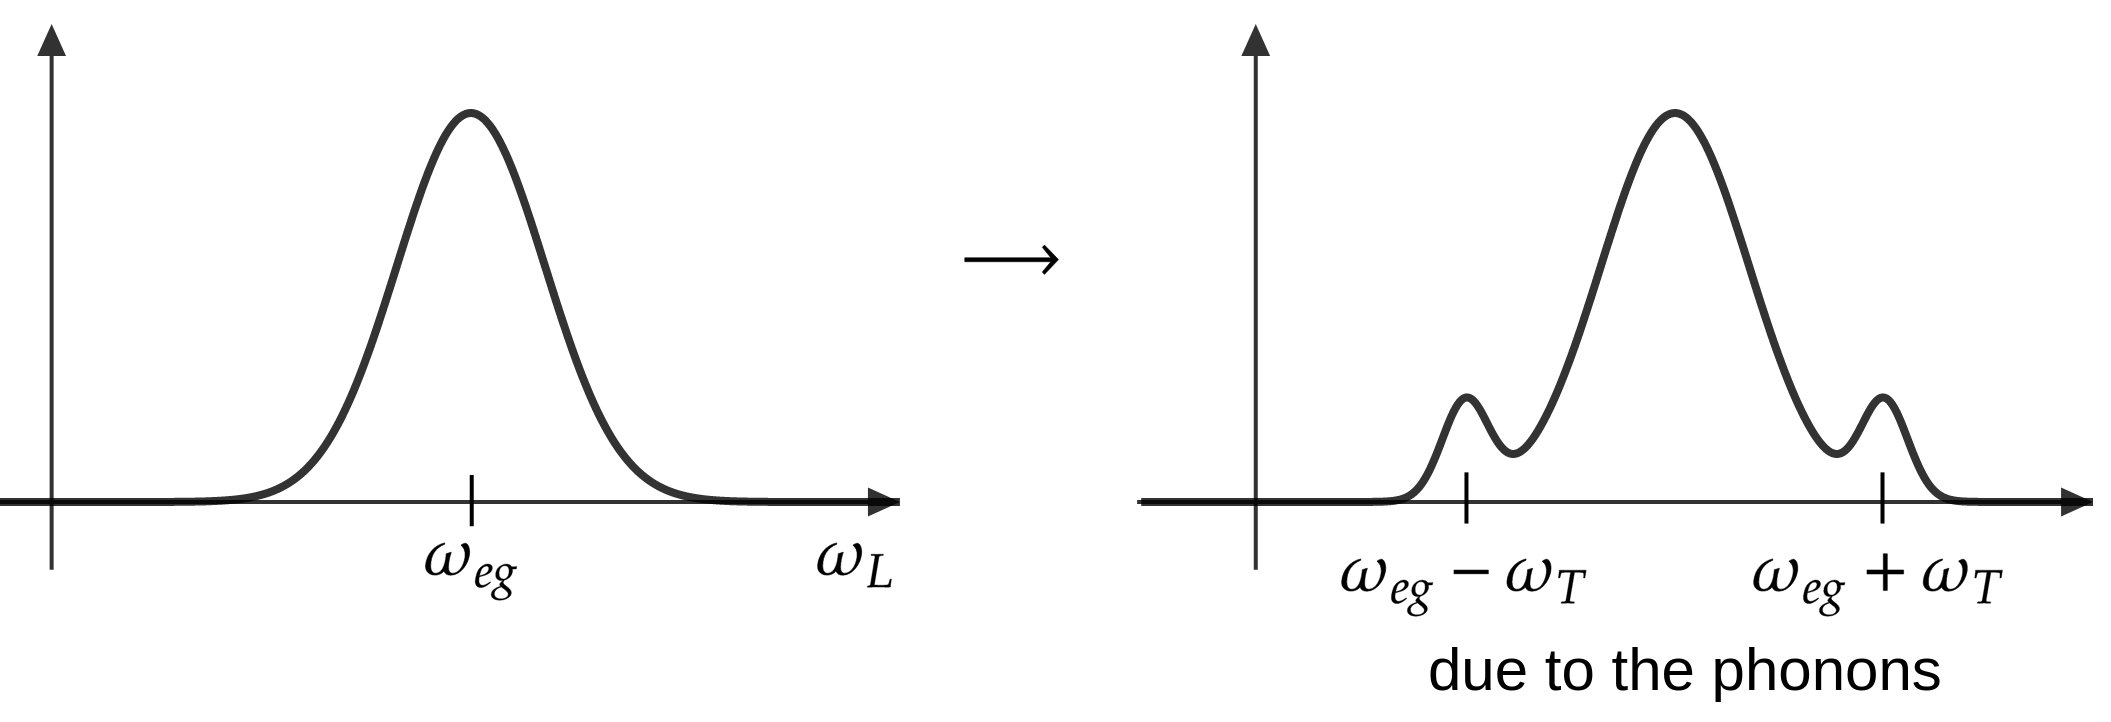
\includegraphics[height=4cm]{img/dicke-red-plot.png}
\end{center}

\subsubsection{Sideband coupling}

There are three coupling sub-regimes, depending on the frequency to which the laser is tuned and the are represented in figure \ref{fig:sideband-coupling}.We analyze each case separately.
\begin{figure}[H]
    \centering
    

\tikzset{every picture/.style={line width=0.75pt}} %set default line width to 0.75pt        

\begin{tikzpicture}[x=0.75pt,y=0.75pt,yscale=-1,xscale=1]
%uncomment if require: \path (0,176); %set diagram left start at 0, and has height of 176

%Straight Lines [id:da14028990751255077] 
\draw [line width=1.5]    (9.63,51.5) -- (52.63,51.5) ;
%Straight Lines [id:da11175967521568253] 
\draw [color={rgb, 255:red, 255; green, 0; blue, 0 }  ,draw opacity=1 ]   (51.71,60.87) -- (72.46,123.48) ;
\draw [shift={(73.09,125.38)}, rotate = 251.66] [color={rgb, 255:red, 255; green, 0; blue, 0 }  ,draw opacity=1 ][line width=0.75]    (6.56,-1.97) .. controls (4.17,-0.84) and (1.99,-0.18) .. (0,0) .. controls (1.99,0.18) and (4.17,0.84) .. (6.56,1.97)   ;
\draw [shift={(51.08,58.97)}, rotate = 71.66] [color={rgb, 255:red, 255; green, 0; blue, 0 }  ,draw opacity=1 ][line width=0.75]    (6.56,-2.94) .. controls (4.17,-1.38) and (1.99,-0.4) .. (0,0) .. controls (1.99,0.4) and (4.17,1.38) .. (6.56,2.94)   ;
%Straight Lines [id:da29434586221130576] 
\draw [color={rgb, 255:red, 74; green, 144; blue, 226 }  ,draw opacity=1 ]   (116.05,59.38) -- (97.16,122.96) ;
\draw [shift={(96.59,124.88)}, rotate = 286.55] [color={rgb, 255:red, 74; green, 144; blue, 226 }  ,draw opacity=1 ][line width=0.75]    (6.56,-1.97) .. controls (4.17,-0.84) and (1.99,-0.18) .. (0,0) .. controls (1.99,0.18) and (4.17,0.84) .. (6.56,1.97)   ;
\draw [shift={(116.62,57.47)}, rotate = 106.55] [color={rgb, 255:red, 74; green, 144; blue, 226 }  ,draw opacity=1 ][line width=0.75]    (6.56,-2.94) .. controls (4.17,-1.38) and (1.99,-0.4) .. (0,0) .. controls (1.99,0.4) and (4.17,1.38) .. (6.56,2.94)   ;
%Straight Lines [id:da035858476752611446] 
\draw    (82.58,60.47) -- (82.62,123.38) ;
\draw [shift={(82.63,125.38)}, rotate = 269.96] [color={rgb, 255:red, 0; green, 0; blue, 0 }  ][line width=0.75]    (6.56,-1.97) .. controls (4.17,-0.84) and (1.99,-0.18) .. (0,0) .. controls (1.99,0.18) and (4.17,0.84) .. (6.56,1.97)   ;
\draw [shift={(82.58,58.47)}, rotate = 89.96] [color={rgb, 255:red, 0; green, 0; blue, 0 }  ][line width=0.75]    (6.56,-2.94) .. controls (4.17,-1.38) and (1.99,-0.4) .. (0,0) .. controls (1.99,0.4) and (4.17,1.38) .. (6.56,2.94)   ;
%Straight Lines [id:da790497420088156] 
\draw  [dash pattern={on 0.84pt off 2.51pt}]  (0,51.5) -- (130.38,51.5) ;
%Straight Lines [id:da9900161263211081] 
\draw [line width=1.5]    (62.63,36.5) -- (105.63,36.5) ;
%Straight Lines [id:da18120661834702578] 
\draw [line width=1.5]    (62.63,129) -- (105.63,129) ;
%Straight Lines [id:da3376964100631521] 
\draw [line width=1.5]    (169.63,51.5) -- (212.63,51.5) ;
%Straight Lines [id:da217953660823897] 
\draw [color={rgb, 255:red, 255; green, 0; blue, 0 }  ,draw opacity=1 ]   (209.42,41.39) -- (232.55,123.45) ;
\draw [shift={(233.09,125.38)}, rotate = 254.26] [color={rgb, 255:red, 255; green, 0; blue, 0 }  ,draw opacity=1 ][line width=0.75]    (6.56,-1.97) .. controls (4.17,-0.84) and (1.99,-0.18) .. (0,0) .. controls (1.99,0.18) and (4.17,0.84) .. (6.56,1.97)   ;
\draw [shift={(208.88,39.47)}, rotate = 74.26] [color={rgb, 255:red, 255; green, 0; blue, 0 }  ,draw opacity=1 ][line width=0.75]    (6.56,-2.94) .. controls (4.17,-1.38) and (1.99,-0.4) .. (0,0) .. controls (1.99,0.4) and (4.17,1.38) .. (6.56,2.94)   ;
%Straight Lines [id:da6608184995861122] 
\draw [color={rgb, 255:red, 74; green, 144; blue, 226 }  ,draw opacity=1 ]   (276.42,43.91) -- (258.04,122.93) ;
\draw [shift={(257.59,124.88)}, rotate = 283.09] [color={rgb, 255:red, 74; green, 144; blue, 226 }  ,draw opacity=1 ][line width=0.75]    (6.56,-1.97) .. controls (4.17,-0.84) and (1.99,-0.18) .. (0,0) .. controls (1.99,0.18) and (4.17,0.84) .. (6.56,1.97)   ;
\draw [shift={(276.88,41.97)}, rotate = 103.09] [color={rgb, 255:red, 74; green, 144; blue, 226 }  ,draw opacity=1 ][line width=0.75]    (6.56,-2.94) .. controls (4.17,-1.38) and (1.99,-0.4) .. (0,0) .. controls (1.99,0.4) and (4.17,1.38) .. (6.56,2.94)   ;
%Straight Lines [id:da13619447520920935] 
\draw    (243.13,41.5) -- (243.13,123.38) ;
\draw [shift={(243.13,125.38)}, rotate = 270] [color={rgb, 255:red, 0; green, 0; blue, 0 }  ][line width=0.75]    (6.56,-1.97) .. controls (4.17,-0.84) and (1.99,-0.18) .. (0,0) .. controls (1.99,0.18) and (4.17,0.84) .. (6.56,1.97)   ;
\draw [shift={(243.13,39.5)}, rotate = 90] [color={rgb, 255:red, 0; green, 0; blue, 0 }  ][line width=0.75]    (6.56,-2.94) .. controls (4.17,-1.38) and (1.99,-0.4) .. (0,0) .. controls (1.99,0.4) and (4.17,1.38) .. (6.56,2.94)   ;
%Straight Lines [id:da8825274475937802] 
\draw  [dash pattern={on 0.84pt off 2.51pt}]  (160,36.5) -- (328.25,36.5) ;
%Straight Lines [id:da4376283057123779] 
\draw [line width=1.5]    (222.63,36.5) -- (265.63,36.5) ;
%Straight Lines [id:da3655084631996305] 
\draw [line width=1.5]    (222.63,129) -- (265.63,129) ;
%Straight Lines [id:da36481720214842805] 
\draw [line width=1.5]    (274.63,20.5) -- (317.63,20.5) ;
%Straight Lines [id:da14498321918646662] 
\draw [color={rgb, 255:red, 255; green, 0; blue, 0 }  ,draw opacity=1 ]   (376.21,25.91) -- (400.16,123.43) ;
\draw [shift={(400.64,125.38)}, rotate = 256.2] [color={rgb, 255:red, 255; green, 0; blue, 0 }  ,draw opacity=1 ][line width=0.75]    (6.56,-1.97) .. controls (4.17,-0.84) and (1.99,-0.18) .. (0,0) .. controls (1.99,0.18) and (4.17,0.84) .. (6.56,1.97)   ;
\draw [shift={(375.73,23.97)}, rotate = 76.2] [color={rgb, 255:red, 255; green, 0; blue, 0 }  ,draw opacity=1 ][line width=0.75]    (6.56,-2.94) .. controls (4.17,-1.38) and (1.99,-0.4) .. (0,0) .. controls (1.99,0.4) and (4.17,1.38) .. (6.56,2.94)   ;
%Straight Lines [id:da7981259927773865] 
\draw [color={rgb, 255:red, 74; green, 144; blue, 226 }  ,draw opacity=1 ]   (448.25,28.41) -- (424.63,122.93) ;
\draw [shift={(424.14,124.88)}, rotate = 284.03] [color={rgb, 255:red, 74; green, 144; blue, 226 }  ,draw opacity=1 ][line width=0.75]    (6.56,-1.97) .. controls (4.17,-0.84) and (1.99,-0.18) .. (0,0) .. controls (1.99,0.18) and (4.17,0.84) .. (6.56,1.97)   ;
\draw [shift={(448.73,26.47)}, rotate = 104.03] [color={rgb, 255:red, 74; green, 144; blue, 226 }  ,draw opacity=1 ][line width=0.75]    (6.56,-2.94) .. controls (4.17,-1.38) and (1.99,-0.4) .. (0,0) .. controls (1.99,0.4) and (4.17,1.38) .. (6.56,2.94)   ;
%Straight Lines [id:da035896781940746525] 
\draw    (410.68,26.97) -- (410.68,123.38) ;
\draw [shift={(410.68,125.38)}, rotate = 270] [color={rgb, 255:red, 0; green, 0; blue, 0 }  ][line width=0.75]    (6.56,-1.97) .. controls (4.17,-0.84) and (1.99,-0.18) .. (0,0) .. controls (1.99,0.18) and (4.17,0.84) .. (6.56,1.97)   ;
\draw [shift={(410.68,24.97)}, rotate = 90] [color={rgb, 255:red, 0; green, 0; blue, 0 }  ][line width=0.75]    (6.56,-2.94) .. controls (4.17,-1.38) and (1.99,-0.4) .. (0,0) .. controls (1.99,0.4) and (4.17,1.38) .. (6.56,2.94)   ;
%Straight Lines [id:da07315183718019935] 
\draw  [dash pattern={on 0.84pt off 2.51pt}]  (360,20.5) -- (495.8,20.5) ;
%Straight Lines [id:da886475154974947] 
\draw [line width=1.5]    (390.18,36.5) -- (433.18,36.5) ;
%Straight Lines [id:da021693587273391435] 
\draw [line width=1.5]    (390.18,129) -- (433.18,129) ;
%Straight Lines [id:da5682832670921795] 
\draw [line width=1.5]    (442.18,20.5) -- (485.18,20.5) ;

% Text Node
\draw (6.63,33.9) node [anchor=north west][inner sep=0.75pt]  [font=\footnotesize]  {$\ket{e,n-1}$};
% Text Node
\draw (67.63,133.4) node [anchor=north west][inner sep=0.75pt]  [font=\footnotesize]  {$\ket{g,n}$};
% Text Node
\draw (21.13,82.9) node [anchor=north west][inner sep=0.75pt]    {$\eta\Omega a$};
% Text Node
\draw (227.63,133.4) node [anchor=north west][inner sep=0.75pt]  [font=\footnotesize]  {$\ket{g,n}$};
% Text Node
\draw (227.63,18.9) node [anchor=north west][inner sep=0.75pt]  [font=\footnotesize]  {$\ket{e,n}$};
% Text Node
\draw (247.13,64.9) node [anchor=north west][inner sep=0.75pt]    {$\Omega $};
% Text Node
\draw (395.18,133.4) node [anchor=north west][inner sep=0.75pt]  [font=\footnotesize]  {$\ket{g,n}$};
% Text Node
\draw (437.68,2.4) node [anchor=north west][inner sep=0.75pt]  [font=\footnotesize]  {$\ket{e,n+1}$};
% Text Node
\draw (442.18,79.9) node [anchor=north west][inner sep=0.75pt]    {$\eta\Omega a^{\dagger }$};
% Text Node
\draw (83.84,157) node [anchor=north] [inner sep=0.75pt]   [align=left] {RED SB};
% Text Node
\draw (243.64,157) node [anchor=north] [inner sep=0.75pt]   [align=left] {CARRIER};
% Text Node
\draw (411.64,155) node [anchor=north] [inner sep=0.75pt]   [align=left] {BLUE SB};


\end{tikzpicture}

    \caption{The three sub-regimes of sideband coupling.}
    \label{fig:sideband-coupling}
\end{figure}


\begin{enumerate}
    \item[1)] \textbf{Carrier resonance} ($\Delta = 0$, or at least $\Delta \ll \omega_T$)\\
    In this regime, the laser is resonant with the direct transition $\Delta \ll \omega_T$ (and weak $\eta\Omega \ll \omega_T$). In particular, there is no coupling between $\ket{g,n}$ and $\ket{e, n\pm 1}$, because by construction $|\omega_T \pm \Delta| \approx \omega_T \;\gg\; \eta\Omega$ . The Hamiltonian is approximately
\begin{equation*}
H_\text{carrier} = \hbar\omega_Ta^\dag a
\;-\;
\hbar\Delta\ket{e}\bra{e}
\;+\;
\frac{\hbar\Omega}{2}\sigma^x 
\sim \begin{pmatrix}
0&\Omega/2 \\
\Omega/2&\omega_T
\end{pmatrix}
\end{equation*}
having used the basis $\{\ket{g,n}, \ket{e, n+1}\}$ to write the matrix elements.

\item[2)] \textbf{Red sideband} ($\Delta \simeq -\omega_T$, or at least $|\omega_L - (\omega_{eg}-\omega_T)| \ll \omega_T$) \\ 
In this case, the laser is resonant with $\omega_{eg} -\omega_T$. We also require that $\Omega \ll \omega_T$.
The denomination ``red" is due to the fact that laser is detuned to a lower frequency (hence more ``red") than carrier. In practice, we ignore the direct and the blue transition, considering only couples $\ket{g,n} \longleftrightarrow \ket{e, n-1}$, as shown in the following figure. 
\begin{center}
    

\tikzset{every picture/.style={line width=0.75pt}} %set default line width to 0.75pt        

\begin{tikzpicture}[x=0.75pt,y=0.75pt,yscale=-1,xscale=1]
%uncomment if require: \path (0,158); %set diagram left start at 0, and has height of 158

%Shape: Axis 2D [id:dp8431562196616039] 
\draw  (0,138) -- (318.17,138)(9.85,6) -- (9.85,148.38) (311.17,133) -- (318.17,138) -- (311.17,143) (4.85,13) -- (9.85,6) -- (14.85,13)  ;
%Straight Lines [id:da5651762429163826] 
\draw [line width=1.5]    (30,125) -- (75,125) ;
%Straight Lines [id:da16666480216181523] 
\draw [color={rgb, 255:red, 255; green, 0; blue, 0 }  ,draw opacity=1 ]   (65.09,38.6) -- (102.5,110.29) ;
\draw [shift={(103.42,112.06)}, rotate = 242.44] [color={rgb, 255:red, 255; green, 0; blue, 0 }  ,draw opacity=1 ][line width=0.75]    (6.56,-1.97) .. controls (4.17,-0.84) and (1.99,-0.18) .. (0,0) .. controls (1.99,0.18) and (4.17,0.84) .. (6.56,1.97)   ;
\draw [shift={(64.17,36.82)}, rotate = 62.44] [color={rgb, 255:red, 255; green, 0; blue, 0 }  ,draw opacity=1 ][line width=0.75]    (6.56,-2.94) .. controls (4.17,-1.38) and (1.99,-0.4) .. (0,0) .. controls (1.99,0.4) and (4.17,1.38) .. (6.56,2.94)   ;
%Straight Lines [id:da9273633131691024] 
\draw [line width=1.5]    (30,30) -- (75,30) ;
%Straight Lines [id:da8337269026387355] 
\draw [line width=1.5]    (100,120) -- (145,120) ;
%Straight Lines [id:da41032876729774204] 
\draw [color={rgb, 255:red, 255; green, 0; blue, 0 }  ,draw opacity=1 ]   (135.09,33.6) -- (172.5,105.29) ;
\draw [shift={(173.42,107.06)}, rotate = 242.44] [color={rgb, 255:red, 255; green, 0; blue, 0 }  ,draw opacity=1 ][line width=0.75]    (6.56,-1.97) .. controls (4.17,-0.84) and (1.99,-0.18) .. (0,0) .. controls (1.99,0.18) and (4.17,0.84) .. (6.56,1.97)   ;
\draw [shift={(134.17,31.82)}, rotate = 62.44] [color={rgb, 255:red, 255; green, 0; blue, 0 }  ,draw opacity=1 ][line width=0.75]    (6.56,-2.94) .. controls (4.17,-1.38) and (1.99,-0.4) .. (0,0) .. controls (1.99,0.4) and (4.17,1.38) .. (6.56,2.94)   ;
%Straight Lines [id:da7310518864520119] 
\draw [line width=1.5]    (100,25) -- (145,25) ;
%Straight Lines [id:da3116124591913111] 
\draw [line width=1.5]    (170,115) -- (215,115) ;
%Straight Lines [id:da12641083556456256] 
\draw [color={rgb, 255:red, 255; green, 0; blue, 0 }  ,draw opacity=1 ]   (205.09,28.6) -- (242.5,100.29) ;
\draw [shift={(243.42,102.06)}, rotate = 242.44] [color={rgb, 255:red, 255; green, 0; blue, 0 }  ,draw opacity=1 ][line width=0.75]    (6.56,-1.97) .. controls (4.17,-0.84) and (1.99,-0.18) .. (0,0) .. controls (1.99,0.18) and (4.17,0.84) .. (6.56,1.97)   ;
\draw [shift={(204.17,26.82)}, rotate = 62.44] [color={rgb, 255:red, 255; green, 0; blue, 0 }  ,draw opacity=1 ][line width=0.75]    (6.56,-2.94) .. controls (4.17,-1.38) and (1.99,-0.4) .. (0,0) .. controls (1.99,0.4) and (4.17,1.38) .. (6.56,2.94)   ;
%Straight Lines [id:da5597533072353611] 
\draw [line width=1.5]    (170,20) -- (215,20) ;
%Straight Lines [id:da38450978230425914] 
\draw [line width=1.5]    (240,110) -- (285,110) ;

% Text Node
\draw (50.67,69.46) node [anchor=north west][inner sep=0.75pt]    {$\eta\Omega $};
% Text Node
\draw (106.17,55.96) node [anchor=north west][inner sep=0.75pt]    {$\eta\Omega \sqrt{2}$};
% Text Node
\draw (174.17,50.96) node [anchor=north west][inner sep=0.75pt]    {$\eta\Omega \sqrt{3}$};


\end{tikzpicture}

\end{center}
The Hamiltonian in this case is
\begin{equation*}
\Rightarrow H_{\text{red}} = \hbar\omega_Ta^\dag a
-
\hbar\Delta\ket{e}\bra{e}
+
\eta\frac{\hbar\Omega}{2}
\left(-i\sigma_+a+i\sigma_-a^\dag\right), 
\end{equation*}
which is the Jaynes-Cummings model (between phonon and level $e$). The difference with respect to the cavity is that the last contribution can be turned off, as the system is controlled by the laser.

\item[3)] \textbf{Blue sideband} ($\Delta \simeq +\omega_T$, or at least $|\omega_L - (\omega_{eg}+\omega_T)| \ll \omega_T$) \\
In this case, the laser is resonant with $\omega_{eg} +\omega_T$. We also require that $\Omega \ll \omega_T$. \\
We can check the energy scales for typical optical systems:
$$\underbrace{|\omega_L -(\omega_{eg}+\omega_T)|}_
{\sim \text{kHz}}
\ll
\underbrace{\omega_T}_{\text{MHz}},$$
The Hamiltonian in this regime is 
\begin{equation*}
\Rightarrow H_{\text{blue}} = \hbar\omega_Ta^\dag a
-
\hbar\Delta\ket{e}\bra{e}
+
\frac{\eta\hbar\Omega}{2}
\left(-i\sigma_+a^\dag+i\sigma_-a\right).
\end{equation*}
It is called ``anti"-Jaynes-Cummings model. 

\begin{center}


\tikzset{every picture/.style={line width=0.75pt}} %set default line width to 0.75pt        

\begin{tikzpicture}[x=0.75pt,y=0.75pt,yscale=-1,xscale=1]
%uncomment if require: \path (0,158); %set diagram left start at 0, and has height of 158

%Shape: Axis 2D [id:dp15618946884319262] 
\draw  (0,138) -- (318.17,138)(9.85,6) -- (9.85,148.38) (311.17,133) -- (318.17,138) -- (311.17,143) (4.85,13) -- (9.85,6) -- (14.85,13)  ;
%Straight Lines [id:da5633161593663423] 
\draw [line width=1.5]    (30,125) -- (75,125) ;
%Straight Lines [id:da6891482979787938] 
\draw [color={rgb, 255:red, 74; green, 144; blue, 226 }  ,draw opacity=1 ]   (107.95,33.65) -- (70.6,116.01) ;
\draw [shift={(69.77,117.83)}, rotate = 294.39] [color={rgb, 255:red, 74; green, 144; blue, 226 }  ,draw opacity=1 ][line width=0.75]    (6.56,-1.97) .. controls (4.17,-0.84) and (1.99,-0.18) .. (0,0) .. controls (1.99,0.18) and (4.17,0.84) .. (6.56,1.97)   ;
\draw [shift={(108.77,31.83)}, rotate = 114.39] [color={rgb, 255:red, 74; green, 144; blue, 226 }  ,draw opacity=1 ][line width=0.75]    (6.56,-2.94) .. controls (4.17,-1.38) and (1.99,-0.4) .. (0,0) .. controls (1.99,0.4) and (4.17,1.38) .. (6.56,2.94)   ;
%Straight Lines [id:da5552335178166578] 
\draw [line width=1.5]    (30,30) -- (75,30) ;
%Straight Lines [id:da6891740634193314] 
\draw [line width=1.5]    (100,120) -- (145,120) ;
%Straight Lines [id:da5661851604865566] 
\draw [line width=1.5]    (100,25) -- (145,25) ;
%Straight Lines [id:da6022612634715885] 
\draw [line width=1.5]    (170,115) -- (215,115) ;
%Straight Lines [id:da9393350496146184] 
\draw [line width=1.5]    (170,20) -- (215,20) ;
%Straight Lines [id:da2934899407823195] 
\draw [line width=1.5]    (235,15) -- (280,15) ;
%Straight Lines [id:da3308284960238893] 
\draw [color={rgb, 255:red, 74; green, 144; blue, 226 }  ,draw opacity=1 ]   (180.95,27.15) -- (143.6,109.51) ;
\draw [shift={(142.77,111.33)}, rotate = 294.39] [color={rgb, 255:red, 74; green, 144; blue, 226 }  ,draw opacity=1 ][line width=0.75]    (6.56,-1.97) .. controls (4.17,-0.84) and (1.99,-0.18) .. (0,0) .. controls (1.99,0.18) and (4.17,0.84) .. (6.56,1.97)   ;
\draw [shift={(181.77,25.33)}, rotate = 114.39] [color={rgb, 255:red, 74; green, 144; blue, 226 }  ,draw opacity=1 ][line width=0.75]    (6.56,-2.94) .. controls (4.17,-1.38) and (1.99,-0.4) .. (0,0) .. controls (1.99,0.4) and (4.17,1.38) .. (6.56,2.94)   ;
%Straight Lines [id:da6178275915895299] 
\draw [color={rgb, 255:red, 74; green, 144; blue, 226 }  ,draw opacity=1 ]   (248.45,22.65) -- (211.1,105.01) ;
\draw [shift={(210.27,106.83)}, rotate = 294.39] [color={rgb, 255:red, 74; green, 144; blue, 226 }  ,draw opacity=1 ][line width=0.75]    (6.56,-1.97) .. controls (4.17,-0.84) and (1.99,-0.18) .. (0,0) .. controls (1.99,0.18) and (4.17,0.84) .. (6.56,1.97)   ;
\draw [shift={(249.27,20.83)}, rotate = 114.39] [color={rgb, 255:red, 74; green, 144; blue, 226 }  ,draw opacity=1 ][line width=0.75]    (6.56,-2.94) .. controls (4.17,-1.38) and (1.99,-0.4) .. (0,0) .. controls (1.99,0.4) and (4.17,1.38) .. (6.56,2.94)   ;

% Text Node
\draw (52.67,69.46) node [anchor=north west][inner sep=0.75pt]    {$\eta\Omega $};
% Text Node
\draw (108.17,55.96) node [anchor=north west][inner sep=0.75pt]    {$\eta\Omega \sqrt{2}$};
% Text Node
\draw (176.17,50.96) node [anchor=north west][inner sep=0.75pt]    {$\eta\Omega \sqrt{3}$};


\end{tikzpicture}

\end{center}

\end{enumerate}


\begin{tcolorbox} [breakable, enhanced]
\textbf{{Some observations about the effective Rabi frequency}} \\
Frequencies mismatch is an issue when designing multi-qubit gates on ion traps: asynchrony requires perfect cooling (or any other workaround). Indeed, if one considers traps in the order of MHz, the temperatures must be really low: 1 MHz $\simeq 48\mu$K. \\
The red sideband can be efficiently used to cool-down atom vibrations, as it reduces the effective number of phonon spontaneously (\textit{phonon drift}).
\end{tcolorbox}


\section{Two atoms in a linear trap}
%\marginnote{This is actually a path towards ion-qubit\\ (trapped ion)\\ quantum computation.}

\begin{center}
    

\tikzset{every picture/.style={line width=0.75pt}} %set default line width to 0.75pt        

\begin{tikzpicture}[x=0.75pt,y=0.75pt,yscale=-1,xscale=1]
%uncomment if require: \path (0,109); %set diagram left start at 0, and has height of 109

%Pentagon Arrow [id:dp794168685774739] 
\draw   (4,43.62) -- (57.06,43.62) -- (76.3,52.26) -- (57.06,60.91) -- (4,60.91) -- cycle ;
%Shape: Ellipse [id:dp04697411659497153] 
\draw   (133.29,53.85) .. controls (133.29,50.74) and (138.81,48.21) .. (145.63,48.21) .. controls (152.45,48.21) and (157.98,50.74) .. (157.98,53.85) .. controls (157.98,56.97) and (152.45,59.5) .. (145.63,59.5) .. controls (138.81,59.5) and (133.29,56.97) .. (133.29,53.85) -- cycle ;
%Shape: Ellipse [id:dp8824898187216484] 
\draw   (137.46,63.35) .. controls (135.19,61.28) and (136.99,55.36) .. (141.51,50.12) .. controls (146.02,44.88) and (151.52,42.3) .. (153.8,44.36) .. controls (156.08,46.42) and (154.27,52.35) .. (149.76,57.59) .. controls (145.25,62.83) and (139.74,65.41) .. (137.46,63.35) -- cycle ;
%Shape: Ellipse [id:dp13173681950698235] 
\draw   (136.81,44.99) .. controls (138.94,42.77) and (144.62,44.93) .. (149.49,49.82) .. controls (154.36,54.71) and (156.58,60.49) .. (154.45,62.71) .. controls (152.32,64.94) and (146.65,62.78) .. (141.78,57.89) .. controls (136.91,52.99) and (134.69,47.22) .. (136.81,44.99) -- cycle ;

%Rounded Rect [id:dp743242906420414] 
\draw  [fill={rgb, 255:red, 255; green, 255; blue, 255 }  ,fill opacity=1 ] (260.29,27.84) .. controls (260.29,26.49) and (259.2,25.41) .. (257.86,25.41) -- (88.56,25.41) .. controls (87.22,25.41) and (86.13,26.49) .. (86.13,27.84) -- (86.13,27.84) .. controls (86.13,29.18) and (87.22,30.27) .. (88.56,30.27) -- (257.86,30.27) .. controls (259.2,30.27) and (260.29,29.18) .. (260.29,27.84) -- cycle ;
%Shape: Ellipse [id:dp96829721697133] 
\draw   (203.55,53.82) .. controls (203.55,50.7) and (209.08,48.17) .. (215.9,48.17) .. controls (222.72,48.17) and (228.24,50.7) .. (228.24,53.82) .. controls (228.24,56.94) and (222.72,59.47) .. (215.9,59.47) .. controls (209.08,59.47) and (203.55,56.94) .. (203.55,53.82) -- cycle ;
%Shape: Ellipse [id:dp14893138861753885] 
\draw   (207.73,63.31) .. controls (205.45,61.25) and (207.26,55.33) .. (211.77,50.08) .. controls (216.28,44.84) and (221.79,42.26) .. (224.07,44.33) .. controls (226.35,46.39) and (224.54,52.31) .. (220.03,57.56) .. controls (215.51,62.8) and (210.01,65.38) .. (207.73,63.31) -- cycle ;
%Shape: Ellipse [id:dp9581768791328901] 
\draw   (207.08,44.96) .. controls (209.21,42.73) and (214.88,44.89) .. (219.75,49.79) .. controls (224.62,54.68) and (226.84,60.45) .. (224.72,62.68) .. controls (222.59,64.91) and (216.91,62.75) .. (212.04,57.85) .. controls (207.17,52.96) and (204.95,47.19) .. (207.08,44.96) -- cycle ;

%Rounded Rect [id:dp04110522752915269] 
\draw  [color={rgb, 255:red, 95; green, 95; blue, 95 }  ,draw opacity=1 ][fill={rgb, 255:red, 255; green, 255; blue, 255 }  ,fill opacity=1 ] (285.21,17.78) .. controls (285.21,16.44) and (284.12,15.35) .. (282.78,15.35) -- (113.48,15.35) .. controls (112.14,15.35) and (111.05,16.44) .. (111.05,17.78) -- (111.05,17.78) .. controls (111.05,19.12) and (112.14,20.21) .. (113.48,20.21) -- (282.78,20.21) .. controls (284.12,20.21) and (285.21,19.12) .. (285.21,17.78) -- cycle ;
%Pentagon Arrow [id:dp587265405222459] 
\draw   (366.57,61.18) -- (313.52,61.18) -- (294.27,52.54) -- (313.52,43.89) -- (366.57,43.89) -- cycle ;
%Rounded Rect [id:dp2560808105145962] 
\draw  [fill={rgb, 255:red, 255; green, 255; blue, 255 }  ,fill opacity=1 ] (260.29,82.64) .. controls (260.29,81.3) and (259.2,80.21) .. (257.86,80.21) -- (88.56,80.21) .. controls (87.22,80.21) and (86.13,81.3) .. (86.13,82.64) -- (86.13,82.64) .. controls (86.13,83.98) and (87.22,85.07) .. (88.56,85.07) -- (257.86,85.07) .. controls (259.2,85.07) and (260.29,83.98) .. (260.29,82.64) -- cycle ;
%Rounded Rect [id:dp3099051608838199] 
\draw  [color={rgb, 255:red, 95; green, 95; blue, 95 }  ,draw opacity=1 ][fill={rgb, 255:red, 255; green, 255; blue, 255 }  ,fill opacity=1 ] (285.21,72.59) .. controls (285.21,71.25) and (284.12,70.16) .. (282.78,70.16) -- (113.48,70.16) .. controls (112.14,70.16) and (111.05,71.25) .. (111.05,72.59) -- (111.05,72.59) .. controls (111.05,73.93) and (112.14,75.02) .. (113.48,75.02) -- (282.78,75.02) .. controls (284.12,75.02) and (285.21,73.93) .. (285.21,72.59) -- cycle ;

% Text Node
\draw (88.13,86.04) node [anchor=north west][inner sep=0.75pt]  [font=\tiny]  {$++++$};
% Text Node
\draw (258.72,61.45) node [anchor=north west][inner sep=0.75pt]  [font=\tiny]  {$----$};
% Text Node
\draw (109.55,54.79) node [anchor=north west][inner sep=0.75pt]  [font=\scriptsize]  {$Ca^{+}$};
% Text Node
\draw (257.77,5.8) node [anchor=north west][inner sep=0.75pt]  [font=\tiny]  {$++++$};
% Text Node
\draw (88.13,31.24) node [anchor=north west][inner sep=0.75pt]  [font=\tiny]  {$----$};
% Text Node
\draw (227.75,55.51) node [anchor=north west][inner sep=0.75pt]  [font=\scriptsize]  {$Ca^{+}$};
% Text Node
\draw (25.32,62.13) node [anchor=north west][inner sep=0.75pt]   [align=left] {{\footnotesize tip}};


\end{tikzpicture}

\end{center}

Consider the same trap used for the single ion (with a quadrupolar confining potential which effectively tights any atom to the $xy$ plane). If one puts two (identical) ions inside the trap, they crystallize due to their equal charge.
The Hamiltonian that describes the system is 
\begin{equation}
\label{eq:atomsharmonic}
H \;=\;
\frac{(p_1^z)^2+(p_2^z)^2}{2m}
\;+\;
\underbrace{\frac{1}{2}m\omega_T^2(z_1^2+z_2^2)}
_{\text{trap on }{z}}
\;+\;
\underbrace{\frac{e^2 Z_{\text{eff}}^2
}{4\pi \varepsilon_0|z_1-z_2|}}
_{\text{Coulomb repulsion}}
\end{equation}
In particular, $Z_{\text{eff}}=1$ for any single-ionised atom. \\ 
There is no analytical exact solution to this problem. Nevertheless, one can solve a simpler classical problem, for instance under the hypothesis of small oscillations, and prove ``a posteriori" that the solution is consistent.

The fist step is a translation of the coordinates about the \textit{classical equilibrium position}
$\bar{z}_j$:
\begin{equation*}
\hat{z}_j \rightarrow \hat{z}_j' - \bar{z}_j\mathds{1}
\end{equation*}
Notice that $\bar{z}_j$ is just a number, not an operator, and that the commutation rules are preserved, i.e. $[z_i',p_j]=[z_i,p_j]+\bar{z}\cancel{[\mathbb{1},p_j]} = [z_i,p_j]$. \\
Since the two atoms are crystallized, one can choose which atom has the greater $z_i$ coordinate and orient $\vec{z}$ such that 
$$\bar{z}_1 > \bar{z}_2 \qquad \implies \qquad \frac{1}{|z_1-z_2|} \xrightarrow[]{z_1>z_2} \frac{1}{z_1-z_2} \;\;.$$

Let us find $\bar{z}_1$ and $\bar{z}_2$.
On the hypothesis of \textit{classical equilibrium}, for a generic coordinate $q_j$ it is
\begin{align*}
\dot{p}_j = 0\qquad \implies \qquad
0 = -\dot{p}_j = \frac{\partial H}{\partial q_j}
\end{align*}
from which, in the $z_j$ coordinates,
\begin{align}
\label{eq:atomsmoments}
\frac{\partial H}{\partial z_j} \bigg\rvert_{\bar{z}_j} = 0
\;\;\Rightarrow\;\;
\begin{cases}
    m\omega_T^2\bar{z}_1 -\dfrac{e^2}{4\pi\varepsilon_0(\bar{z}_1-\bar{z}_2)^2} = 0\\
    m\omega_T^2\bar{z}_2 + \dfrac{e^2}{4\pi\varepsilon_0(\bar{z}_1-\bar{z}_2)^2} = 0
\end{cases}
\end{align}
Summing the equations, one gets easily that $\bar{z}_1=-\bar{z}_2$. Substituting back, the first equation reads
\begin{equation}
\label{eq:atomssymmetrycond}
m\omega_T^2\bar{z}_1 = \frac{e^2}{4\pi\varepsilon_0}\frac{1}{4\bar{z}_1^2}
\qquad \implies \qquad
\bar{z}_1 = 
\left( \frac{e^2}{16\pi\varepsilon_0m\omega_T^2} \right)^{1/3} = -\bar{z}_2
\end{equation}
Now we want to rewrite Eq. \ref{eq:atomsharmonic} in prime coordinates. The coordinates of the Coulombian term can be expanded for small oscillations as
\begin{equation*}
|\hat{z}_1-\hat{z}_2|^{-1} \equalexpl{$z_1>z_2$}
(\hat{z}_1-\hat{z}_2)^{-1} \simeq
\frac{\mathds{1}}{\hat{z}_1-\hat{z}_2}
-\frac{\hat{z}_1'-\hat{z}_2'}{(\bar{z}_1-\bar{z}_2)^2}
+\frac{\cancel{2}}{\cancel{2}}\frac{(\hat{z}_1'-\hat{z}_2')^2}{(\bar{z}_1-\bar{z}_2)^3}
+{O}(\hat{z}_j^{\prime\;3})
\end{equation*}
whereas the trap term requires the square of the coordinates, which is
\begin{equation*}
\hat{z}_j = \hat{z}_j' + \bar{z}_j\mathds{1}
\qquad\implies\qquad
\hat{z}_j^2 = \hat{z}_j^{\prime\;2} +
2\bar{z}_j\hat{z}_j^\prime +
\bar{z}_j^2\mathds{1} \;\;.
\end{equation*}
Shifting away the constants, one ends up with the Hamiltonian 
\begin{align}
\begin{split}
H_{\substack{\text{small} \\ \text{oscill.}}} = \; &
\frac{(p_1^z)^2+(p_2^z)^2}{2m}
\;+ \\
& +\; \frac{m\omega_T^2}{2}
    \left(
        \cancel{\bar{z}_1^2\mathds{1}} + \cancel{\bar{z}_2^2\mathds{1}}
        + 2 \bar{z}_1\hat{z}_1' + 2 \bar{z}_2\hat{z}_2'
        + \hat{z}_1^{\prime\;2} + \hat{z}_2^{\prime\;2}
    \right) \;+ \\
& +\;
\frac{e^2}{4\pi \varepsilon_0}
\left(
    \cancel{\frac{\mathds{1}}{ \hat{z}_1-\hat{z}_2 }}       - \frac{\hat{z}_1'-\hat{z}_2'}{(\hat{z}_1-\hat{z}_2)^2}
        + \frac{(\hat{z}_1'-\hat{z}_2')^2}{(\hat{z}_1-\hat{z}_2)^3}
\right)
+{O}(\hat{z}_j^{\prime\;3})
\end{split}
\end{align}
Further simplifications can be done isolating the terms by their order:
\begin{itemize}
    \item at first order in the prime coordinates, because of Equations \ref{eq:atomsmoments}
    \begin{equation*}
    (I) \qquad \longrightarrow \qquad
        \hat{z}_1' \underbrace{
            \left(
                m\omega_T^2\bar{z}_1 - \frac{e^2}{4\pi\varepsilon_0(4\bar{z}_1^2)} 
            \right)
        }_{=0} + \hat{z}_2' \underbrace{
            \left(
                m\omega_T^2\bar{z}_2 + \frac{e^2}{4\pi\varepsilon_0(4\bar{z}_2^2)} 
            \right)
        }_{=0} = 0
    \end{equation*}
    Not surprisingly... this quantity is null by construction.
    
    \item at second order
    \begin{equation*}
    (II) \qquad \longrightarrow \qquad
    \frac{m\omega_T^2}{2}
    \left( \hat{z}_1^{\prime\;2} + \hat{z}_2^{\prime\;2}  \right)
    +
    \left( \hat{z}_1^{\prime\;2} - \hat{z}_2^{\prime\;2} \right)
    {\frac{e^2}{4\pi\varepsilon_0}(\bar{z}_1-\bar{z}_2)^{-3}}
    \end{equation*}
    where, because of Eq. \ref{eq:atomssymmetrycond},
    \begin{equation*}
    \frac{e^2}{4\pi\varepsilon_0}(\bar{z}_1-\bar{z}_2)^{-3} =
    \frac{e^2}{4\pi\varepsilon_0}\frac{1}{8\bar{z}_1^3} =
    \frac{e^2}{32\pi\varepsilon_0}
    \left(
        \frac{16\pi\varepsilon_0m\omega^2_T}{e^2}
    \right) = \frac{1}{2}m\omega_T^2
    \end{equation*}
\end{itemize}
Combining the simplifications,
\begin{align}
\label{eq:atoms-harmonic-coupled}
H_{\substack{\text{small} \\ \text{oscill.}}} = 
\frac{(p_1^z)^2+(p_2^z)^2}{2m}
+
 \frac{m\omega_T^2}{2}
    \left(
        \hat{z}_1^{\prime\;2} + \hat{z}_2^{\prime\;2}
        + \left( \hat{z}_1'-\hat{z}_1' \right)^2
    \right)
    + {O}\left( z_j^3 \right)
\end{align}
This Hamiltonian describes two coupled harmonic oscillators. One can define this new set of coordinates
\begin{equation}
\text{CoM}: \begin{dcases}
Z=\frac{z_1'+z_2'}{2}\\P=p_1^z+p_2^z
\end{dcases}
\qquad \qquad 
\text{Relative}: \begin{dcases}
z=z_1-z_2\\p = \frac{p^z_1-p^z_2}{2}
\end{dcases}
\end{equation}
which inverts as
\begin{equation*}
\label{eq:inverted-coords-coupled}
p_{1,2}^z = \frac{P}{2}\pm p \qquad \qquad z'_{1,2} = Z\pm\frac{z}{2}
\end{equation*}
The terms of Equation \ref{eq:atoms-harmonic-coupled} can be written using the new coordinates
\begin{equation*}
(p_{1}^z)^2 + (p_{2}^z)^2 = \frac{P^2}{2} + 2p^2 \;,
\qquad 
(z'_1)^2 + (z'_2)^2 = 2Z^2 + \frac{z^2}{2} \;,
\qquad \text{and} \qquad
(z'_1 - z'_2)^2 = z^2.
\end{equation*}
These coordinates are really convenient, because the new Hamiltonian is the sum of two decoupled problems:
\begin{equation}
\label{eq:twoatoms-harmonic-modes}
H_{\substack{\text{small} \\ \text{oscill.}}} = 
\underbrace{\left[ \frac{P^2}{4m}+m\omega_T^2Z^2 \right]}
_{\text{CoM harmonic oscillator}}
+ 
\underbrace{\left[\frac{p^2}{m}+\frac{m\omega_T^2}{2}\left(\frac{3z^2}{2}\right)\right]}
_{\text{Stretch mode harmonic oscillator}}
+ \;\;{O}\left( z_j^3 \right)
\end{equation}


% define the dotted arrows
\def\bulletrightarrow{\hbox{$\bullet$}\kern-2pt\hbox{$\rightarrow$}}
\def\bulletleftarrow{\hbox{$\leftarrow$}\kern-2pt\hbox{$\bullet$}}


\noindent To solve this problem, one moves to the ladder operators formalism for each the two normal modes of the decoupled harmonic oscillators:
\begin{itemize}

    \item \textbf{CoM mode}
    $\qquad \left( \substack{
        \bulletrightarrow \; \; \bulletrightarrow \\ 
        \bulletleftarrow  \; \; \bulletleftarrow } \right)$
    \begin{align*}
    \begin{dcases}
        Z = \sqrt{\frac{\hbar}{4m\omega_T}}
            \left(  a_{CoM} + a_{CoM}^\dag \right)\\
        P = i\sqrt{\hbar m\omega_T}
            \left(  a_{CoM}^\dag - a_{CoM} \right)
    \end{dcases}
    \;\;\Leftrightarrow\;\; a_{CoM} = \sqrt{\frac{m\omega_T}{\hbar}}\;Z+
            i\sqrt{\frac{1}{4\hbar m\omega_T}}\;P
    \end{align*}

    \item \textbf{Stretch mode}
    $\qquad \left( \substack{ 
        \bulletrightarrow \; \; \bulletleftarrow \\
        \bulletleftarrow  \; \; \bulletrightarrow } \right)$
    \begin{align*}
    \begin{dcases}
        z = \sqrt{\frac{\hbar}{\sqrt{3}m\omega_T}}
            \left(  a_{S} + a_{S}^\dag \right)\\
        p = i\sqrt{\frac{\sqrt{3}\hbar m\omega_T}{4}}
            \left(  a_{S}^\dag - a_{S} \right)
    \end{dcases}
    \;\;\Leftrightarrow \;\;
    a_{S} = \sqrt{\frac{\sqrt{3}m\omega_T}{4\hbar}}\;z+
            i\sqrt{\frac{1}{\sqrt{3}\hbar m\omega_T}}\;p
    \end{align*}
\end{itemize}
This leads to an utterly simplified form of equation (\ref{eq:twoatoms-harmonic-modes}):
\begin{align}
\label{eq:twoatoms-ladder-harmonic-modes}
H_{\substack{\text{small} \\ \text{oscill.}}} = \hbar\omega_T
    \left( a_{CoM}^\dag a_{CoM} + \cancel{\frac{1}{2}} \right) +
    \hbar\sqrt{3}\omega_T
    \left( a_{S}^\dag a_{S} + \cancel{\frac{1}{2}} \right)
    + \cancel{\mathcal{O}\left( \dots \right)},
\end{align}
where the constant terms have been removed. We also see that the stretch mode is $\sqrt{3} \simeq 1.73$ times faster than $CoM$ mode, that is, several MHz away.

At the end of the day, one can recover the laboratory coordinates of the two atoms with $z_{1,2}=\pm\bar{z}_1+z'_{1,2} = \pm \bar{z}_1 + Z \pm \frac{z}{2}$,
\begin{equation}
\label{eq:lab-coords}
z_{1,2} =
    \pm\bar{z}
    + \sqrt{\frac{\hbar}{4m\omega_T}}
        \left( a_{CoM} + a_{CoM}^\dag \right)
    \pm \sqrt{\frac{\hbar}{4\sqrt{3}m\omega_T}}
        \left( a_S + a_S^\dag \right)
\end{equation}
and observe that their distance is orders of magnitude greater than the atom size. This means that the two atoms are sufficiently ``far away'', so one can suppose to be able to hit specifically one of them with a laser. Which is exactly what we will do!

%\begin{figure}[h!]
%\centering
%    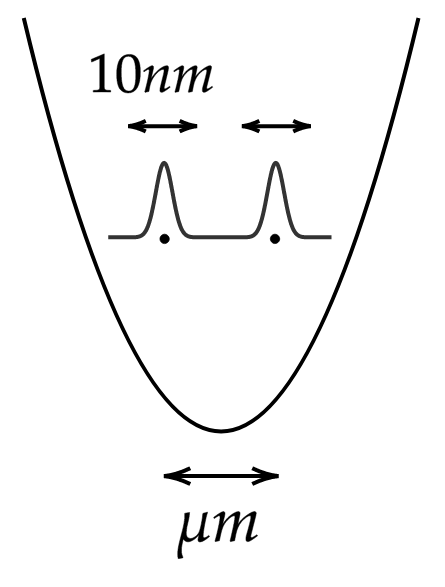
\includegraphics[width=0.3\linewidth]{img/sketch_far_atoms.png}
%\end{figure}


\subsection{Two trapped atoms under a focused laser}

\marginnote{From now on, we will shorten $CoM$ with $C$.}
Suppose to focus a laser, say, on ion 1 (of coordinate $z_1$). The Hamiltonian of such system would be composed by the one of equation (\ref{eq:twoatoms-ladder-harmonic-modes}), plus a dipole light-atom coupling term $H_{AL} = -\vec{d}\cdot\vec{E}(\vec{r})$:
\begin{equation}
H^{lab} = 
\underbrace{
\hbar \omega_Ta_{C}^\dag a_{C}
+
\sqrt{3}\hbar\omega_Ta_S^\dag a_S
}_{\ref{eq:twoatoms-ladder-harmonic-modes}}
+ \hbar\Omega\sum_j\ket{e}\bra{e}_j + H_{AL}
\end{equation}
where
\begin{align*}
H_{AL} &= -\hbar\Omega\ket{e}\bra{g}_1
\cos\left(ckt-\cos\theta kz_1\right) + \text{h.c.}
\end{align*}
can be rewritten using equation (\ref{eq:lab-coords})
\begin{align*}
    H_{AL} = -\hbar\Omega\ket{e}\bra{g}_1 \cos
\bigg(&
    ckt -
    \underbrace{\cos\theta k\bar{z}_1}_{\phi_0}
    -\underbrace{\cos\theta k \sqrt{\frac{\hbar}{4m\omega_T}}}
        _{\eta_{C}}
    (a_{C}+a^\dag_{C}) + \\
    &-\underbrace{\cos\theta k \sqrt{\frac{\hbar}{4\sqrt{3}m\omega_T}}}
        _{\eta_{S}}
    (a_{S}+a^\dag_{S})
\bigg)
+ \text{h.c.}
\end{align*}
Consider the rotating-wave approximation 
$$|\omega_{eg}-\omega_L|,\Omega \;\ll\; \omega_{eg},\omega_L$$
and in the rotating frame, defined by the transformation
$U(t) = e^{-i\omega_L t\sum_j\ket{e}\bra{e}_j + i \phi_0}$. The Hamiltonian becomes
\begin{align*}
\begin{split}
H^{rot}_{RWA} =\; &
\hbar \overbrace{\left(\omega_{eg}-\omega_{L}\right)}
    ^{\equiv-\Delta}
\sum_j \ket{e}\bra{e}_j 
+
\hbar \omega_{T}a_{C}^\dag a_{C}
+
\sqrt{3}\hbar\omega_Ta_S^\dag a_S
+\\
& -\frac{\hbar\Omega}{2}\ket{e}\bra{g}_1
e^{-i\eta_{C}(a+a^\dag)_{C}}
e^{-i\eta_{S}(a+a^\dag)_{S}}
+ \text{h.c.}
\end{split}
\end{align*}
Using the hypothesis that the $\eta$s are small parameters (Lamb-Dicke regime)
\begin{align*}
    e^{-i\eta_{C}(a+a^\dag)_{C}}
    e^{-i\eta_{S}(a+a^\dag)_{S}}
    = 1 
    - i\eta_{C}(a_{C}+a_{C}^\dag) 
    - i\eta_{S}(a_{S}+a_{S}^\dag) 
    + \mathcal{O}(\eta^2) \;\;,
\end{align*}
the final result is
\begin{align}
\begin{split}
H^{rot}_{RWA} =\; &
-\hbar\Delta
\sum_j \ket{e}\bra{e}_j 
+
\hbar \omega_{T}a_{C}^\dag a_{C}
+
\sqrt{3}\hbar\omega_Ta_S^\dag a_S
+\\
& -\frac{\hbar\Omega}{2}\ket{e}\bra{g}_1
\left(
1 - i\eta_{C}(a_{C}+a_{C}^\dag)
- i\eta_{S}(a_{S}+a_{S}^\dag)
+{O}(\eta^2)
\right)
+ \text{h.c.}
\end{split}
\end{align}

From an experimental point of view, it would be possible to tune the laser to a specific sideband of a specific mode. Consider, for instance, the red sideband of CoM mode reported in the following figure: 
\begin{center}
    

\tikzset{every picture/.style={line width=0.75pt}} %set default line width to 0.75pt        

\begin{tikzpicture}[x=0.75pt,y=0.75pt,yscale=-1,xscale=1]
%uncomment if require: \path (0,146); %set diagram left start at 0, and has height of 146

%Straight Lines [id:da8993089849930328] 
\draw    (30.38,59.59) -- (82.31,59.59) ;
%Straight Lines [id:da29699103187525655] 
\draw    (30.38,30.75) -- (82.31,30.75) ;
%Straight Lines [id:da9565575071502495] 
\draw    (93.89,130.93) -- (145.83,130.93) ;
%Straight Lines [id:da38723274535804597] 
\draw    (93.89,9.5) -- (145.83,9.5) ;
%Straight Lines [id:da7230830907382644] 
\draw    (87.59,12.14) -- (87.59,26.36) ;
\draw [shift={(87.59,28.36)}, rotate = 270] [color={rgb, 255:red, 0; green, 0; blue, 0 }  ][line width=0.75]    (4.37,-1.32) .. controls (2.78,-0.56) and (1.32,-0.12) .. (0,0) .. controls (1.32,0.12) and (2.78,0.56) .. (4.37,1.32)   ;
\draw [shift={(87.59,10.14)}, rotate = 90] [color={rgb, 255:red, 0; green, 0; blue, 0 }  ][line width=0.75]    (4.37,-1.32) .. controls (2.78,-0.56) and (1.32,-0.12) .. (0,0) .. controls (1.32,0.12) and (2.78,0.56) .. (4.37,1.32)   ;
%Straight Lines [id:da7613574342882506] 
\draw    (97.98,14.06) -- (97.98,55.96) ;
\draw [shift={(97.98,57.96)}, rotate = 270] [color={rgb, 255:red, 0; green, 0; blue, 0 }  ][line width=0.75]    (4.37,-1.32) .. controls (2.78,-0.56) and (1.32,-0.12) .. (0,0) .. controls (1.32,0.12) and (2.78,0.56) .. (4.37,1.32)   ;
\draw [shift={(97.98,12.06)}, rotate = 90] [color={rgb, 255:red, 0; green, 0; blue, 0 }  ][line width=0.75]    (4.37,-1.32) .. controls (2.78,-0.56) and (1.32,-0.12) .. (0,0) .. controls (1.32,0.12) and (2.78,0.56) .. (4.37,1.32)   ;
%Straight Lines [id:da17453665512381966] 
\draw [color={rgb, 255:red, 255; green, 0; blue, 0 }  ,draw opacity=1 ]   (78.43,38.62) -- (105.81,126.62) ;
\draw [shift={(106.4,128.53)}, rotate = 252.72] [color={rgb, 255:red, 255; green, 0; blue, 0 }  ,draw opacity=1 ][line width=0.75]    (6.56,-1.97) .. controls (4.17,-0.84) and (1.99,-0.18) .. (0,0) .. controls (1.99,0.18) and (4.17,0.84) .. (6.56,1.97)   ;
\draw [shift={(77.84,36.71)}, rotate = 72.72] [color={rgb, 255:red, 255; green, 0; blue, 0 }  ,draw opacity=1 ][line width=0.75]    (6.56,-1.97) .. controls (4.17,-0.84) and (1.99,-0.18) .. (0,0) .. controls (1.99,0.18) and (4.17,0.84) .. (6.56,1.97)   ;
%Straight Lines [id:da35411700829971027] 
\draw    (287,12) -- (287,128) ;
\draw [shift={(287,130)}, rotate = 270] [color={rgb, 255:red, 0; green, 0; blue, 0 }  ][line width=0.75]    (8.74,-2.63) .. controls (5.56,-1.12) and (2.65,-0.24) .. (0,0) .. controls (2.65,0.24) and (5.56,1.12) .. (8.74,2.63)   ;
\draw [shift={(287,10)}, rotate = 90] [color={rgb, 255:red, 0; green, 0; blue, 0 }  ][line width=0.75]    (8.74,-2.63) .. controls (5.56,-1.12) and (2.65,-0.24) .. (0,0) .. controls (2.65,0.24) and (5.56,1.12) .. (8.74,2.63)   ;
%Straight Lines [id:da3640218170366485] 
\draw    (230,13.8) -- (230,32.55) ;
\draw [shift={(230,34.55)}, rotate = 270] [color={rgb, 255:red, 0; green, 0; blue, 0 }  ][line width=0.75]    (6.56,-1.97) .. controls (4.17,-0.84) and (1.99,-0.18) .. (0,0) .. controls (1.99,0.18) and (4.17,0.84) .. (6.56,1.97)   ;
\draw [shift={(230,11.8)}, rotate = 90] [color={rgb, 255:red, 0; green, 0; blue, 0 }  ][line width=0.75]    (6.56,-1.97) .. controls (4.17,-0.84) and (1.99,-0.18) .. (0,0) .. controls (1.99,0.18) and (4.17,0.84) .. (6.56,1.97)   ;

% Text Node
\draw (153,123.4) node [anchor=north west][inner sep=0.75pt]  [font=\footnotesize]  {$\ket{g,n_{C} ,n_{S}}$};
% Text Node
\draw (153,3.4) node [anchor=north west][inner sep=0.75pt]  [font=\footnotesize]  {$\ket{e,n_{C} ,n_{S}}$};
% Text Node
\draw (57,10.9) node [anchor=north west][inner sep=0.75pt]  [font=\footnotesize]  {$-\omega _{T}$};
% Text Node
\draw (102.5,28.9) node [anchor=north west][inner sep=0.75pt]  [font=\footnotesize]  {$-\sqrt{3} \omega _{T}$};
% Text Node
\draw (5,16) node [anchor=north west][inner sep=0.75pt]  [font=\footnotesize] [align=left] {red C};
% Text Node
\draw (5,44.5) node [anchor=north west][inner sep=0.75pt]  [font=\footnotesize] [align=left] {red S};
% Text Node
\draw (290,64.63) node [anchor=north west][inner sep=0.75pt]  [font=\scriptsize]  {$ >THz$};
% Text Node
\draw (234,16.43) node [anchor=north west][inner sep=0.75pt]  [font=\scriptsize]  {$\sim MHz$};
% Text Node
\draw (101,83.63) node [anchor=north west][inner sep=0.75pt]  [font=\footnotesize,color={rgb, 255:red, 255; green, 0; blue, 0 }  ,opacity=1 ]  {$\eta_C \Omega \sqrt{n_{C}}$};


\end{tikzpicture}

\end{center}

The detuning is sufficiently large to make it possible and the stretch mode will not be excited. Indeed, if
\begin{align*}
\text{KHz} \approx |\Delta + \omega_T| \ll \omega_T \approx \text{MHz}
\end{align*}
but
\begin{align*}
|\Delta\pm\sqrt{3}\omega_T| & \approx | -\omega_T \pm \sqrt{3}\omega_T| \approx\\
& \approx |\sqrt{3}\pm1|\omega_T  \;
\underbrace{\;> 0.7 \cdot \omega_T \;\approx \text{MHz}}_{ \mathclap{\text{far detuned ($\Rightarrow$ no excitation of stretch mode)}} }
\end{align*}

\noindent The Hamiltonian would be a center-of-mass (axial) phonon Jaynes-Cummings model:
\begin{align}
\begin{split}
H_{red} = & -\hbar(\omega_T +\varepsilon)
    \ket{e}\bra{e}_1 
    \;+\;
    \hbar \omega_{T}a_{C}^\dag a_{C}
    \;+ \\
& +\frac{\hbar\eta_{C}\Omega}{2}
\left( i\sigma_1^+a_{C} - i\sigma_1^-a_{C} \right)
\;\; + \text{decoupled stuff}
\end{split}
\end{align}
having defined $|\omega_L-\omega_{eg}+\omega_T| = \varepsilon \ll \omega_T$. 

\vspace{1cm}
\begin{tcolorbox}[breakable, enhanced]
\textbf{Summary}\\

Let us briefly recap the take-away message of this section. We have considered two atoms in a trap with two focused laser beams. We have found that the dynamics of the system is described by two modes.
\begin{equation*}
\text{construction}\;\; \left( \substack{
        \bulletrightarrow \; \; \bulletrightarrow \\ 
        \bulletleftarrow  \; \; \bulletleftarrow } \right)
\qquad\qquad
\text{destruction}\;\;
\left( \substack{ 
        \bulletrightarrow \; \; \bulletleftarrow \\
        \bulletleftarrow  \; \; \bulletrightarrow } \right)
\end{equation*}
which create a phonon structure, like the one seen in previous paragraphs, but separable on each mode:
\begin{center}
    

\tikzset{every picture/.style={line width=0.75pt}} %set default line width to 0.75pt        

\begin{tikzpicture}[x=0.75pt,y=0.75pt,yscale=-1,xscale=1]
%uncomment if require: \path (0,146); %set diagram left start at 0, and has height of 146

%Straight Lines [id:da8993089849930328] 
\draw    (30.38,59.59) -- (82.31,59.59) ;
%Straight Lines [id:da29699103187525655] 
\draw    (30.38,30.75) -- (82.31,30.75) ;
%Straight Lines [id:da9565575071502495] 
\draw    (93.89,130.93) -- (145.83,130.93) ;
%Straight Lines [id:da38723274535804597] 
\draw    (93.89,9.5) -- (145.83,9.5) ;
%Straight Lines [id:da7230830907382644] 
\draw    (87.59,12.14) -- (87.59,26.36) ;
\draw [shift={(87.59,28.36)}, rotate = 270] [color={rgb, 255:red, 0; green, 0; blue, 0 }  ][line width=0.75]    (4.37,-1.32) .. controls (2.78,-0.56) and (1.32,-0.12) .. (0,0) .. controls (1.32,0.12) and (2.78,0.56) .. (4.37,1.32)   ;
\draw [shift={(87.59,10.14)}, rotate = 90] [color={rgb, 255:red, 0; green, 0; blue, 0 }  ][line width=0.75]    (4.37,-1.32) .. controls (2.78,-0.56) and (1.32,-0.12) .. (0,0) .. controls (1.32,0.12) and (2.78,0.56) .. (4.37,1.32)   ;
%Straight Lines [id:da7613574342882506] 
\draw    (97.98,14.06) -- (97.98,55.96) ;
\draw [shift={(97.98,57.96)}, rotate = 270] [color={rgb, 255:red, 0; green, 0; blue, 0 }  ][line width=0.75]    (4.37,-1.32) .. controls (2.78,-0.56) and (1.32,-0.12) .. (0,0) .. controls (1.32,0.12) and (2.78,0.56) .. (4.37,1.32)   ;
\draw [shift={(97.98,12.06)}, rotate = 90] [color={rgb, 255:red, 0; green, 0; blue, 0 }  ][line width=0.75]    (4.37,-1.32) .. controls (2.78,-0.56) and (1.32,-0.12) .. (0,0) .. controls (1.32,0.12) and (2.78,0.56) .. (4.37,1.32)   ;
%Straight Lines [id:da17453665512381966] 
\draw [color={rgb, 255:red, 255; green, 0; blue, 0 }  ,draw opacity=1 ]   (78.43,38.62) -- (105.81,126.62) ;
\draw [shift={(106.4,128.53)}, rotate = 252.72] [color={rgb, 255:red, 255; green, 0; blue, 0 }  ,draw opacity=1 ][line width=0.75]    (6.56,-1.97) .. controls (4.17,-0.84) and (1.99,-0.18) .. (0,0) .. controls (1.99,0.18) and (4.17,0.84) .. (6.56,1.97)   ;
\draw [shift={(77.84,36.71)}, rotate = 72.72] [color={rgb, 255:red, 255; green, 0; blue, 0 }  ,draw opacity=1 ][line width=0.75]    (6.56,-1.97) .. controls (4.17,-0.84) and (1.99,-0.18) .. (0,0) .. controls (1.99,0.18) and (4.17,0.84) .. (6.56,1.97)   ;
%Straight Lines [id:da35411700829971027] 
\draw    (287,12) -- (287,128) ;
\draw [shift={(287,130)}, rotate = 270] [color={rgb, 255:red, 0; green, 0; blue, 0 }  ][line width=0.75]    (8.74,-2.63) .. controls (5.56,-1.12) and (2.65,-0.24) .. (0,0) .. controls (2.65,0.24) and (5.56,1.12) .. (8.74,2.63)   ;
\draw [shift={(287,10)}, rotate = 90] [color={rgb, 255:red, 0; green, 0; blue, 0 }  ][line width=0.75]    (8.74,-2.63) .. controls (5.56,-1.12) and (2.65,-0.24) .. (0,0) .. controls (2.65,0.24) and (5.56,1.12) .. (8.74,2.63)   ;
%Straight Lines [id:da3640218170366485] 
\draw    (230,13.8) -- (230,32.55) ;
\draw [shift={(230,34.55)}, rotate = 270] [color={rgb, 255:red, 0; green, 0; blue, 0 }  ][line width=0.75]    (6.56,-1.97) .. controls (4.17,-0.84) and (1.99,-0.18) .. (0,0) .. controls (1.99,0.18) and (4.17,0.84) .. (6.56,1.97)   ;
\draw [shift={(230,11.8)}, rotate = 90] [color={rgb, 255:red, 0; green, 0; blue, 0 }  ][line width=0.75]    (6.56,-1.97) .. controls (4.17,-0.84) and (1.99,-0.18) .. (0,0) .. controls (1.99,0.18) and (4.17,0.84) .. (6.56,1.97)   ;

% Text Node
\draw (153,123.4) node [anchor=north west][inner sep=0.75pt]  [font=\footnotesize]  {$\ket{g,n_{C} ,n_{S}}$};
% Text Node
\draw (153,3.4) node [anchor=north west][inner sep=0.75pt]  [font=\footnotesize]  {$\ket{e,n_{C} ,n_{S}}$};
% Text Node
\draw (57,10.9) node [anchor=north west][inner sep=0.75pt]  [font=\footnotesize]  {$-\omega _{T}$};
% Text Node
\draw (102.5,28.9) node [anchor=north west][inner sep=0.75pt]  [font=\footnotesize]  {$-\sqrt{3} \omega _{T}$};
% Text Node
\draw (5,16) node [anchor=north west][inner sep=0.75pt]  [font=\footnotesize] [align=left] {red C};
% Text Node
\draw (5,44.5) node [anchor=north west][inner sep=0.75pt]  [font=\footnotesize] [align=left] {red S};
% Text Node
\draw (290,64.63) node [anchor=north west][inner sep=0.75pt]  [font=\scriptsize]  {$ >THz$};
% Text Node
\draw (234,16.43) node [anchor=north west][inner sep=0.75pt]  [font=\scriptsize]  {$\sim MHz$};
% Text Node
\draw (101,83.63) node [anchor=north west][inner sep=0.75pt]  [font=\footnotesize,color={rgb, 255:red, 255; green, 0; blue, 0 }  ,opacity=1 ]  {$\eta_C \Omega \sqrt{n_{C}}$};


\end{tikzpicture}

\end{center}

\end{tcolorbox}
\vspace{1cm}




\section{Example: Cirac-Zoller CNOT gate}

We want to build a CNOT gate for two qubits. This step is fundamental to get a universal set of operations.\\

\noindent \textbf{Ingredients}:
\begin{itemize}
    \item $2 \times$ 3-level $\{\ket{g}, \ket{e}, \ket{a}\}$ trapped ions (ex: $Ca^+$), where the auxiliary state $\ket{a}$ is not an allowed input.
    \item $2 \times$ focused lasers $L1, L2$ which can be rapidly turned on/off.
    \item $1 \times$ harmonic ion trap.
\end{itemize}
\begin{center}
    

\tikzset{every picture/.style={line width=0.75pt}} %set default line width to 0.75pt        

\begin{tikzpicture}[x=0.75pt,y=0.75pt,yscale=-1,xscale=1]
%uncomment if require: \path (0,162); %set diagram left start at 0, and has height of 162

%Shape: Parabola [id:dp6600560249897834] 
\draw   (13.11,11.18) .. controls (67.39,173.84) and (121.68,173.84) .. (175.97,11.18) ;
%Shape: Circle [id:dp18474882329925513] 
\draw   (60,101.7) .. controls (60,99.66) and (61.66,98) .. (63.7,98) .. controls (65.75,98) and (67.41,99.66) .. (67.41,101.7) .. controls (67.41,103.75) and (65.75,105.41) .. (63.7,105.41) .. controls (61.66,105.41) and (60,103.75) .. (60,101.7) -- cycle ;
%Shape: Circle [id:dp1125926223428434] 
\draw   (120,101.7) .. controls (120,99.66) and (121.66,98) .. (123.7,98) .. controls (125.75,98) and (127.41,99.66) .. (127.41,101.7) .. controls (127.41,103.75) and (125.75,105.41) .. (123.7,105.41) .. controls (121.66,105.41) and (120,103.75) .. (120,101.7) -- cycle ;
%Shape: Parabola [id:dp9511655488027904] 
\draw  [color={rgb, 255:red, 255; green, 187; blue, 0 }  ,draw opacity=1 ] (31.42,135.12) .. controls (51.71,113.31) and (66.23,88.17) .. (74.97,59.69) ;
%Shape: Parabola [id:dp36759296152967846] 
\draw  [color={rgb, 255:red, 255; green, 187; blue, 0 }  ,draw opacity=1 ] (93.8,71.19) .. controls (73.51,93.01) and (59,118.15) .. (50.25,146.62) ;
%Shape: Parabola [id:dp36811618670172386] 
\draw  [color={rgb, 255:red, 74; green, 144; blue, 226 }  ,draw opacity=1 ] (90.42,137.12) .. controls (110.71,115.31) and (125.23,90.17) .. (133.97,61.69) ;
%Shape: Parabola [id:dp18893194431896954] 
\draw  [color={rgb, 255:red, 74; green, 144; blue, 226 }  ,draw opacity=1 ] (152.8,73.19) .. controls (132.51,95.01) and (118,120.15) .. (109.25,148.62) ;
%Straight Lines [id:da2309226656139074] 
\draw    (74,30) -- (54,30) ;
%Rounded Rect [id:dp3741809575727877] 
\draw   (60.5,16.28) .. controls (60.5,15.57) and (61.07,15) .. (61.78,15) -- (65.63,15) .. controls (66.33,15) and (66.91,15.57) .. (66.91,16.28) -- (66.91,66.89) .. controls (66.91,67.6) and (66.33,68.18) .. (65.63,68.18) -- (61.78,68.18) .. controls (61.07,68.18) and (60.5,67.6) .. (60.5,66.89) -- cycle ;
%Straight Lines [id:da9684575061600806] 
\draw    (74,50) -- (54,50) ;
%Straight Lines [id:da9880508830624835] 
\draw    (134.5,29.5) -- (114.5,29.5) ;
%Rounded Rect [id:dp6621821890356242] 
\draw   (121,15.78) .. controls (121,15.07) and (121.57,14.5) .. (122.28,14.5) -- (126.13,14.5) .. controls (126.83,14.5) and (127.41,15.07) .. (127.41,15.78) -- (127.41,66.39) .. controls (127.41,67.1) and (126.83,67.68) .. (126.13,67.68) -- (122.28,67.68) .. controls (121.57,67.68) and (121,67.1) .. (121,66.39) -- cycle ;
%Straight Lines [id:da20298612962713958] 
\draw    (134.5,49.5) -- (114.5,49.5) ;

% Text Node
\draw (29,138) node [anchor=north west][inner sep=0.75pt]   [align=left] {{\small \textcolor[rgb]{1,0.73,0}{L1}}};
% Text Node
\draw (88,137.5) node [anchor=north west][inner sep=0.75pt]  [color={rgb, 255:red, 74; green, 144; blue, 226 }  ,opacity=1 ] [align=left] {{\small \textcolor[rgb]{0.29,0.56,0.89}{L2}}};
% Text Node
\draw (39.5,54.9) node [anchor=north west][inner sep=0.75pt]  [font=\scriptsize]  {$\ket{g}$};
% Text Node
\draw (39.5,35.4) node [anchor=north west][inner sep=0.75pt]  [font=\scriptsize]  {$\ket{e}$};
% Text Node
\draw (39.5,15.9) node [anchor=north west][inner sep=0.75pt]  [font=\scriptsize]  {$\ket{a}$};
% Text Node
\draw (100,54.4) node [anchor=north west][inner sep=0.75pt]  [font=\scriptsize]  {$\ket{g}$};
% Text Node
\draw (100,34.9) node [anchor=north west][inner sep=0.75pt]  [font=\scriptsize]  {$\ket{e}$};
% Text Node
\draw (100,15.4) node [anchor=north west][inner sep=0.75pt]  [font=\scriptsize]  {$\ket{a}$};


\end{tikzpicture}

\end{center}

We have seen previously that we need a very good cooling strategy too, since we need $CoM$ phonons at $T\sim0$.

\textbf{Remark}: When a laser is perfectly resonant to a transition, I can go to an interaction picture via a suitable frame change $\tilde{U}$ on the hamiltonian $H$. If
\begin{equation*}
H = \begin{pmatrix}
    \ddots\\
    & \varepsilon_1\\
    &&\varepsilon_2&\Omega\\
    &&\Omega& \varepsilon_2\\
    &&&&\varepsilon_3\\
    &&&&&\ddots\\
\end{pmatrix},
\;\;
\tilde{U} = \begin{pmatrix}
    \ddots\\
    & e^{i\varepsilon_1t}\\
    && e^{i\varepsilon_2t}\\
    &&& e^{i\varepsilon_2t}\\
    &&&& e^{i\varepsilon_3t}\\
    &&&&&\ddots\\
\end{pmatrix}
\end{equation*}
we obtain in the interaction picture as $H_{int} = \tilde{U}H\tilde{U} + i\hbar \dot{\tilde{U}}\tilde{U}^\dag$, i.e.
\begin{equation*}
H_{int} = \begin{pmatrix}
    0\\
    & 0\\
    && 0 & \Omega\\
    && \Omega & 0\\
    &&&& 0\\
    &&&&&0\\
\end{pmatrix}
\end{equation*}
$\Rightarrow$ it is convenient to go to the interaction picture in order to perform calculations, as the bare hamiltonian goes away.




\subsection{Protocol}

The lasers are tuned in the following way:
\begin{itemize}
    \item Laser 1 ($L1$) is focused on ion 1, in resonance to $\ket{g}_1 \leftrightarrow \ket{e}_1$ through a red-sideband transition\\
    $$H_{L1} = \frac{\hbar\eta_C\Omega_1(t)}{2}
    \left( i\ket{e}\bra{g}_1 a_C + h.c. \right)$$
    $$\omega_{L1} \approx \omega_{eg} -\omega_T$$
    \item Laser 2 ($L2$) is focused on ion 2, in resonance to $\ket{g}_2 \leftrightarrow \ket{a}_2$ through a red-sideband transition\\
    $$H_{L2} = \frac{\hbar\eta_C\Omega_2(t)}{2}
    \left( i\ket{a}\bra{g}_2a_C + h.c. \right)$$
    $$\omega_{L2} \approx \omega_{ag} -\omega_T$$
\end{itemize}




\noindent In principle the lasers may show some transient when turned on/off. For this protocol one can take the frequency evolution to be similar to a square function (the laser turns on/off immediately). The protocol consists of the following steps:

\begin{itemize}

% STEP 1
\item \textbf{Step 1} - Laser 2 off, Laser 1 on for $t_1 = \frac{\pi}{\eta_C\Omega_1}$. We call this a $\pi$-PULSE. 
    The unitary operator associated to this operation is
    \begin{align*}
    U_1 &= \exp{ -i\frac{\pi}{\eta_C\Omega_1} \frac{1}{\hbar} H_1 }\\% -i or -1 ??? TODO
    & = \exp{ \frac{ -i \pi}{2}
        \left( i \ket{e}\bra{g}_1a_C - i \ket{g}\bra{e}_1a^\dag_C \right)
    }
    \end{align*}
    and it acts basically as $\sigma_y$ on the states $\ket{g_1, 1}$ and $\ket{e_1, 0}$. 
    Indeed, because of
    $e^{i\alpha\sigma_k} = \cos\alpha \mathds{1} + i \sin\alpha \sigma_k$,
    it is $e^{-i\pi\sigma_y/2} = -i \sigma_y$.
    
    In general, the result of the operation is
    \begin{align*}
        \ket{g_1,0} & \overset{U_1}{\longrightarrow} \;\;\; \ket{g_1, 0}\\
        \ket{e_1, 0} & \longrightarrow
            \;\;\; i\left(\ket{e}\bra{g}_1a - \ket{g}\bra{e}_1a^\dag\right)\ket{e_1, 0} = -i \ket{g_1, 1} 
    \end{align*}
    which is graphically represented as
    \begin{center}
    

\tikzset{every picture/.style={line width=0.75pt}} %set default line width to 0.75pt        

\begin{tikzpicture}[x=0.75pt,y=0.75pt,yscale=-1,xscale=1]
%uncomment if require: \path (0,199); %set diagram left start at 0, and has height of 199

%Shape: Axis 2D [id:dp8238200389598417] 
\draw  (48.83,169.89) -- (313.97,169.89)(57.04,3.94) -- (57.04,182.93) (306.97,164.89) -- (313.97,169.89) -- (306.97,174.89) (52.04,10.94) -- (57.04,3.94) -- (62.04,10.94)  ;
%Straight Lines [id:da9816207475534422] 
\draw [line width=1.5]    (79,143) -- (139.47,143) ;
%Straight Lines [id:da5381598078444266] 
\draw [line width=1.5]    (79,50) -- (139.47,50) ;
%Straight Lines [id:da9628952673311713] 
\draw [line width=1.5]    (159,137.5) -- (219.47,137.5) ;
%Straight Lines [id:da8455519996835935] 
\draw [line width=1.5]    (159,44.5) -- (219.47,44.5) ;
%Straight Lines [id:da8044015159070315] 
\draw [line width=1.5]    (239,132.5) -- (299.47,132.5) ;
%Straight Lines [id:da313266698785474] 
\draw [line width=1.5]  [dash pattern={on 1.69pt off 2.76pt}]  (5,56.5) -- (65.47,56.5) ;
%Straight Lines [id:da6553984074417375] 
\draw [color={rgb, 255:red, 255; green, 0; blue, 0 }  ,draw opacity=1 ]   (124.93,56.54) -- (162.33,128.23) ;
\draw [shift={(163.26,130)}, rotate = 242.44] [color={rgb, 255:red, 255; green, 0; blue, 0 }  ,draw opacity=1 ][line width=0.75]    (6.56,-1.97) .. controls (4.17,-0.84) and (1.99,-0.18) .. (0,0) .. controls (1.99,0.18) and (4.17,0.84) .. (6.56,1.97)   ;
\draw [shift={(124,54.77)}, rotate = 62.44] [color={rgb, 255:red, 255; green, 0; blue, 0 }  ,draw opacity=1 ][line width=0.75]    (6.56,-2.94) .. controls (4.17,-1.38) and (1.99,-0.4) .. (0,0) .. controls (1.99,0.4) and (4.17,1.38) .. (6.56,2.94)   ;
%Straight Lines [id:da14779868058376777] 
\draw [color={rgb, 255:red, 255; green, 0; blue, 0 }  ,draw opacity=1 ]   (51.93,64.54) -- (89.33,136.23) ;
\draw [shift={(90.26,138)}, rotate = 242.44] [color={rgb, 255:red, 255; green, 0; blue, 0 }  ,draw opacity=1 ][line width=0.75]    (6.56,-1.97) .. controls (4.17,-0.84) and (1.99,-0.18) .. (0,0) .. controls (1.99,0.18) and (4.17,0.84) .. (6.56,1.97)   ;
\draw [shift={(51,62.77)}, rotate = 62.44] [color={rgb, 255:red, 255; green, 0; blue, 0 }  ,draw opacity=1 ][line width=0.75]    (6.56,-2.94) .. controls (4.17,-1.38) and (1.99,-0.4) .. (0,0) .. controls (1.99,0.4) and (4.17,1.38) .. (6.56,2.94)   ;
%Straight Lines [id:da6792105316737991] 
\draw [color={rgb, 255:red, 255; green, 0; blue, 0 }  ,draw opacity=1 ]   (208.93,51.54) -- (246.33,123.23) ;
\draw [shift={(247.26,125)}, rotate = 242.44] [color={rgb, 255:red, 255; green, 0; blue, 0 }  ,draw opacity=1 ][line width=0.75]    (6.56,-1.97) .. controls (4.17,-0.84) and (1.99,-0.18) .. (0,0) .. controls (1.99,0.18) and (4.17,0.84) .. (6.56,1.97)   ;
\draw [shift={(208,49.77)}, rotate = 62.44] [color={rgb, 255:red, 255; green, 0; blue, 0 }  ,draw opacity=1 ][line width=0.75]    (6.56,-2.94) .. controls (4.17,-1.38) and (1.99,-0.4) .. (0,0) .. controls (1.99,0.4) and (4.17,1.38) .. (6.56,2.94)   ;

% Text Node
\draw (91,147.9) node [anchor=north west][inner sep=0.75pt]    {$\ket{g,0}$};
% Text Node
\draw (91,27.9) node [anchor=north west][inner sep=0.75pt]    {$\ket{e,1}$};
% Text Node
\draw (170.5,141.4) node [anchor=north west][inner sep=0.75pt]    {$\ket{g,1}$};
% Text Node
\draw (21,36) node [anchor=north west][inner sep=0.75pt]  [color={rgb, 255:red, 208; green, 2; blue, 27 }  ,opacity=1 ] [align=left] {??};


\end{tikzpicture}

    \end{center}

\item \textbf{Step 2} - Laser 1 off, Laser 2 on for $t_2 = \frac{2\pi}{\eta_C\Omega_2}$. We call this a $2\pi$-PULSE.
    The unitary transformation is
    \begin{align*}
    \Rightarrow U_2 &= \exp{ -\frac{i}{\hbar}\frac{2\pi}{\eta_C\Omega_2} H_2 }\\
    & = \exp{ -i\pi \left(
        i\ket{a}\bra{g}_2a_C - 
        i\ket{g}\bra{a}_2a_C^\dag
    \right)
    }
    \end{align*}
    
    The expression acts like $-\mathds{1}$ on the states $\ket{g_2,1}, \ket{a_2, 0}$. Given the possible starting states
    \begin{align*}
        \ket{g_2,0} & \overset{U_2}{\longrightarrow} \;\;\; \ket{g_2, 0}\\
        \ket{e_2, 0} & \longrightarrow \;\;\; \ket{e_2, 0}\\
        \ket{g_2, 1} & \longrightarrow - \ket{g_2, 1}
    \end{align*}
    
    \begin{center}
    

\tikzset{every picture/.style={line width=0.75pt}} %set default line width to 0.75pt        

\begin{tikzpicture}[x=0.75pt,y=0.75pt,yscale=-1,xscale=1]
%uncomment if require: \path (0,199); %set diagram left start at 0, and has height of 199

%Shape: Axis 2D [id:dp7044047881463993] 
\draw  (22.83,170.89) -- (287.97,170.89)(31.04,4.94) -- (31.04,183.93) (280.97,165.89) -- (287.97,170.89) -- (280.97,175.89) (26.04,11.94) -- (31.04,4.94) -- (36.04,11.94)  ;
%Straight Lines [id:da8544066902130162] 
\draw [line width=1.5]    (53,144) -- (113.47,144) ;
%Straight Lines [id:da7205922197236949] 
\draw [line width=1.5]    (53,51) -- (113.47,51) ;
%Straight Lines [id:da5372911334007633] 
\draw [line width=1.5]    (133,138.5) -- (193.47,138.5) ;
%Straight Lines [id:da025883166300928573] 
\draw [line width=1.5]    (133,45.5) -- (193.47,45.5) ;
%Straight Lines [id:da8336819480921466] 
\draw [color={rgb, 255:red, 255; green, 0; blue, 0 }  ,draw opacity=1 ]   (98.93,57.54) -- (136.33,129.23) ;
\draw [shift={(137.26,131)}, rotate = 242.44] [color={rgb, 255:red, 255; green, 0; blue, 0 }  ,draw opacity=1 ][line width=0.75]    (6.56,-1.97) .. controls (4.17,-0.84) and (1.99,-0.18) .. (0,0) .. controls (1.99,0.18) and (4.17,0.84) .. (6.56,1.97)   ;
\draw [shift={(98,55.77)}, rotate = 62.44] [color={rgb, 255:red, 255; green, 0; blue, 0 }  ,draw opacity=1 ][line width=0.75]    (6.56,-2.94) .. controls (4.17,-1.38) and (1.99,-0.4) .. (0,0) .. controls (1.99,0.4) and (4.17,1.38) .. (6.56,2.94)   ;
%Straight Lines [id:da8918814843361473] 
\draw [color={rgb, 255:red, 255; green, 0; blue, 0 }  ,draw opacity=1 ]   (25.93,65.54) -- (63.33,137.23) ;
\draw [shift={(64.26,139)}, rotate = 242.44] [color={rgb, 255:red, 255; green, 0; blue, 0 }  ,draw opacity=1 ][line width=0.75]    (6.56,-1.97) .. controls (4.17,-0.84) and (1.99,-0.18) .. (0,0) .. controls (1.99,0.18) and (4.17,0.84) .. (6.56,1.97)   ;
\draw [shift={(25,63.77)}, rotate = 62.44] [color={rgb, 255:red, 255; green, 0; blue, 0 }  ,draw opacity=1 ][line width=0.75]    (6.56,-2.94) .. controls (4.17,-1.38) and (1.99,-0.4) .. (0,0) .. controls (1.99,0.4) and (4.17,1.38) .. (6.56,2.94)   ;
%Straight Lines [id:da2473095698421811] 
\draw [color={rgb, 255:red, 255; green, 0; blue, 0 }  ,draw opacity=1 ]   (188.93,98.54) -- (226.33,170.23) ;
\draw [shift={(227.26,172)}, rotate = 242.44] [color={rgb, 255:red, 255; green, 0; blue, 0 }  ,draw opacity=1 ][line width=0.75]    (6.56,-1.97) .. controls (4.17,-0.84) and (1.99,-0.18) .. (0,0) .. controls (1.99,0.18) and (4.17,0.84) .. (6.56,1.97)   ;
\draw [shift={(188,96.77)}, rotate = 62.44] [color={rgb, 255:red, 255; green, 0; blue, 0 }  ,draw opacity=1 ][line width=0.75]    (6.56,-2.94) .. controls (4.17,-1.38) and (1.99,-0.4) .. (0,0) .. controls (1.99,0.4) and (4.17,1.38) .. (6.56,2.94)   ;
%Straight Lines [id:da5354722999998263] 
\draw [line width=1.5]    (53,96) -- (113.47,96) ;
%Straight Lines [id:da15509678461862553] 
\draw [line width=1.5]    (133,90) -- (193.47,90) ;
%Straight Lines [id:da5426262796400413] 
\draw [color={rgb, 255:red, 255; green, 0; blue, 0 }  ,draw opacity=1 ]   (105.93,105.54) -- (143.33,177.23) ;
\draw [shift={(144.26,179)}, rotate = 242.44] [color={rgb, 255:red, 255; green, 0; blue, 0 }  ,draw opacity=1 ][line width=0.75]    (6.56,-1.97) .. controls (4.17,-0.84) and (1.99,-0.18) .. (0,0) .. controls (1.99,0.18) and (4.17,0.84) .. (6.56,1.97)   ;
\draw [shift={(105,103.77)}, rotate = 62.44] [color={rgb, 255:red, 255; green, 0; blue, 0 }  ,draw opacity=1 ][line width=0.75]    (6.56,-2.94) .. controls (4.17,-1.38) and (1.99,-0.4) .. (0,0) .. controls (1.99,0.4) and (4.17,1.38) .. (6.56,2.94)   ;

% Text Node
\draw (65,148.9) node [anchor=north west][inner sep=0.75pt]    {$\ket{g,0}$};
% Text Node
\draw (145,95.9) node [anchor=north west][inner sep=0.75pt]    {$\ket{e,1}$};
% Text Node
\draw (144.5,142.4) node [anchor=north west][inner sep=0.75pt]    {$\ket{g,1}$};
% Text Node
\draw (2,47) node [anchor=north west][inner sep=0.75pt]  [color={rgb, 255:red, 208; green, 2; blue, 27 }  ,opacity=1 ] [align=left] {??};
% Text Node
\draw (65,101.9) node [anchor=north west][inner sep=0.75pt]    {$\ket{e,0}$};
\draw (65,30) node [anchor=north west][inner sep=0.75pt]    {$\ket{a,0}$};
% Text Node
\draw (146.26,182) node [anchor=north west][inner sep=0.75pt]  [color={rgb, 255:red, 208; green, 2; blue, 27 }  ,opacity=1 ] [align=left] {??};
% Text Node
\draw (228.26,176) node [anchor=north west][inner sep=0.75pt]  [color={rgb, 255:red, 208; green, 2; blue, 27 }  ,opacity=1 ] [align=left] {??};


\end{tikzpicture}

    \end{center}


\item \textbf{Step 3} - Identical to \textit{Step 1}.
    $$\Rightarrow U_3 = U_1$$
    In particular, $U_3\;i\ket{g_1, 1} = + \ket{e_1,0}$.
\end{itemize}


\noindent \textbf{Table of canonical states} - If we consider all the 4 possible inputs, then
\begin{align*}
    \text{Inputs:}\;\;&
    \begin{cases}
        \ket{ g_1, g_2, 0} \\[1pt]
        \ket{ g_1, e_2, 0} \\[1pt]
        \ket{ e_1, g_2, 0} \\[1pt]
        \ket{ e_1, e_2, 0}
    \end{cases}
    \;\; \xrightarrow[L1\;\;\pi]{U_1} \;\;
    \begin{aligned}
        \ket{ g_1, g_2, 0} \\[1pt]
        \ket{ g_1, e_2, 0} \\[1pt]
        - i\ket{ g_1, g_2, 1} \\[1pt]
        - i\ket{ g_1, e_2, 1}
    \end{aligned}
    \;\; \xrightarrow[L2\;\;2\pi]{U_2} \\
    & \xrightarrow{U_2} \;\;
    \begin{aligned}
        \ket{ g_1, g_2, 0} \\[1pt]
        \ket{ g_1, e_2, 0} \\[1pt]
        + i\ket{ g_1, g_2, 1} \\[1pt]
        - i\ket{ g_1, e_2, 1}
    \end{aligned}
    \;\; \xrightarrow[L1\;\;\pi]{U_3=U_1} \qquad
    \text{Outputs:}
    \begin{cases}
        \ket{ g_1, g_2, 0} \\[1pt]
        \ket{ g_1, e_2, 0} \\[1pt]
        \ket{ e_1, g_2, 0} \\[1pt]
        - \ket{ e_1, e_2, 0}
    \end{cases}
\end{align*}

This operation goes from states with zero phonons to other states with zero phonons, but with a switched sign in the fourth input state. Therefore, the protocol acts as a \textbf{control-flip} gate on the second ion (qubit):
\begin{equation*}
    G_{CZ} = U_1 U_2 U_1 = \begin{pmatrix}
        1\\
        &1\\
        &&1\\
        &&&-1
    \end{pmatrix}
    = \begin{quantikz}
        & \ctrl{1} &\qw \\
        & \gate{Z} &\qw \\
    \end{quantikz}
\end{equation*}
from which one can build the CNOT gate as
\begin{center}
$CNOT =\;$
\begin{quantikz}
    & \ctrl{1} &\qw \\
    & \targ{} &\qw \\
\end{quantikz}
$\;\;=\;\;$
\begin{quantikz}
    &\qw      & \ctrl{1} & \qw     &\qw \\
    &\gate{H} & \gate{Z} & \gate{H} &\qw \\
\end{quantikz}
\end{center}

\noindent Being able to create such gate is a fundamental requirement to perform universal quantum computing operations.\\

\noindent \textbf{Note}: The most strict requirement of this protocol is to approach the limit $T=0$ (zero temperature phonon $\sim \mu K$). Some year after Cirac-Zoller\footnote{\href{https://doi.org/10.1103/PhysRevLett.74.4091}{Phys. Rev. Lett. 74, 4091 (1995)} - This is generalized for $N$ ions.} design of a CNOT gate, Klaus Mølmer and Anders Sørensen proposed a solution\footnote{\href{https://doi.org/10.1103/PhysRevLett.82.1971}{Phys. Rev. Lett. 82, 1971 (1999)}} which addressed the strict requirement of the temperature.


\chapter[Quantum Simulation]{Correlated atomic systems and Quantum Simulation}
% -----------------------------------------------------------
%
%  CHAPTER 7  of Quantum information with atoms and photons
%
%  written by Francesco Barone, Jan 2023
%  contributions from Giosuè Sardo Infirri
% -----------------------------------------------------------


\section{Optical lattices} % Prof. Di Liberto

% LECTURE 23 (continue)

Digital quantum simulations require the implementation of gates to execute fundamental operations on the quantum states. Instead, \textbf{analog quantum simulations} aim to map the Hamiltonian of a target system on a quantum simulator system and study its evolution - this idea has been argued as truly revolutionary by R. Feynman, back in 1982. One typical simulator platform is made of ultra-cold atoms in \textbf{optical lattices}. The goal is to understand states of matter and phenomena that cannot be simulated on a classical computer: high-temperature superconductors, quantum phase transitions, fractional quantum Hall effect, anyons, ...


\begin{description}
\setlist[description]{style=nextline}
\setlist[enumerate]{topsep=0pt,before=\leavevmode}

\item[Advantages]
    \begin{enumerate}
        \item One-to-one correspondence
        \item Tunability
        \item No computational errors
    \end{enumerate} 

\item[Disadvantages] 
    \begin{enumerate} 
        \item New simulator for each system model
        \item Experimental capabilities (must find a compromise between temperature, system size, interactions)
    \end{enumerate} 

\item[Advantages]
    \begin{enumerate} 
        \item Encode the degrees of freedom on the quantum simulator
        \item Design state preparation
        \item Readout measurement
    \end{enumerate} 
    
\end{description}


%\begin{table}[h]
%\begin{tabular}{ll}
%\hline
%\multirow{3}{*}{Advantages} & 1 to 1 correspondence \\
% & Tunability \\
% & No computational errors \\ \hline
%\multirow{2}{*}{ Disadvantages} & New simulator for each system model \\
% & Experimental capabilities (temperature, system size, interactions) \\ \hline
%\multirow{3}{*}{Requirements} &  Encode the degrees of freedom on the quantum system\\
% & Design state preparation \\
% & Readout measurement \\ \hline
%\end{tabular}
%\end{table}

\noindent We will address optical lattices using \textbf{ultra-cold atoms}:
\begin{itemize}
    \item get simple models with few parameters
    \item can change particle statistics (ex: $\prescript{6}{}{Li}$ for Fermions, $\prescript{7}{}{Li}, \prescript{87}{}{Rb}, \prescript{23}{}{Na}, ...$ for Bosons)
    \item many methods to implement models and to measure, since it is an `old' field of research
\end{itemize}


\noindent But \textbf{how do we create the lattice}?




\subsection{AC-Stark Shift}

\begin{center}
    

\tikzset{every picture/.style={line width=0.75pt}} %set default line width to 0.75pt        

\begin{tikzpicture}[x=0.75pt,y=0.75pt,yscale=-1,xscale=1]
%uncomment if require: \path (0,121); %set diagram left start at 0, and has height of 121

%Straight Lines [id:da16867782903128048] 
\draw  [dash pattern={on 0.8pt off 2.0pt}]  (34,26) -- (84.97,26) ;
%Straight Lines [id:da39705900807308525] 
\draw    (7,86) -- (57.97,86) ;
%Straight Lines [id:da09910835469997958] 
\draw    (12.07,20.73) -- (12.07,81.36) ;
\draw [shift={(12.07,84.36)}, rotate = 270] [fill={rgb, 255:red, 0; green, 0; blue, 0 }  ][line width=0.08]  [draw opacity=0] (5.36,-2.57) -- (0,0) -- (5.36,2.57) -- cycle    ;
\draw [shift={(12.07,17.73)}, rotate = 90] [fill={rgb, 255:red, 0; green, 0; blue, 0 }  ][line width=0.08]  [draw opacity=0] (5.36,-2.57) -- (0,0) -- (5.36,2.57) -- cycle    ;
%Straight Lines [id:da027548097951511363] 
\draw    (7,16) -- (57.97,16) ;
%Straight Lines [id:da21514573737838005] 
\draw    (54.07,31.93) -- (54.07,80.36) ;
\draw [shift={(54.07,83.36)}, rotate = 270] [fill={rgb, 255:red, 0; green, 0; blue, 0 }  ][line width=0.08]  [draw opacity=0] (5.36,-2.57) -- (0,0) -- (5.36,2.57) -- cycle    ;
\draw [shift={(54.07,28.93)}, rotate = 90] [fill={rgb, 255:red, 0; green, 0; blue, 0 }  ][line width=0.08]  [draw opacity=0] (5.36,-2.57) -- (0,0) -- (5.36,2.57) -- cycle    ;

% Text Node
\draw (64.87,6.5) node [anchor=north west][inner sep=0.75pt]  [font=\small]  {$\ket{e}$};
% Text Node
\draw (64.87,78.55) node [anchor=north west][inner sep=0.75pt]  [font=\small]  {$\ket{g}$};
% Text Node
\draw (16,37.39) node [anchor=north west][inner sep=0.75pt]  [font=\small]  {$\omega _{eg}$};
% Text Node
\draw (58,50.19) node [anchor=north west][inner sep=0.75pt]  [font=\small]  {$\omega _{L}$};


\end{tikzpicture}

\end{center}

The AC Stark shift (or Autler–Townes effect) allows to create an optical lattice. Consider an atom with two energy levels and two counter-propagating laser beams in 1D (linear polarization) forming a standing wave:
%suppose also that laser's $\langle\hat{E}\rangle\sim\vec{\varepsilon}$ and 
\begin{equation*}
\begin{cases}
    \vec{\varepsilon}_1 = \varepsilon_0\cos(kx-\omega t)\vec{x}\\
    \vec{\varepsilon}_2 = \varepsilon_0\cos(-kx-\omega t)\vec{x}
\end{cases}
\end{equation*}
\begin{equation*}
\vec{\varepsilon}
= \vec{\varepsilon}_1 + \vec{\varepsilon}_2
= \vec{x} \underbrace{2\varepsilon_0\cos kx}_{\varepsilon_0(x)} \cos(\omega t) 
\end{equation*}

Let $\delta=\omega_L-\omega_{eg}$. In the condition $E_{kin} \ll \hbar\omega$, we are in the classical regime, therefore
\begin{equation*}
    H = \hbar\delta\ket{e}\bra{e}
    + \frac{\hbar\Omega(x)}{2}\hat{\sigma_x}
    + \left(
        \frac{\hbar\Omega(x)}{2}e^{2i\omega t}
        \sigma_+ 
        + h.c.
    \right)
\end{equation*}
%
and the Rabi frequency is space dependent:
$$\Omega(x) = 
\frac{\vec{d}_{eg}\cdot\vec{x}}{\hbar} 
2\varepsilon_0\cos kx $$

What's the energy of the ground (dressed) state? In the condition $\delta \gg \hbar\Omega(x)$ (large detuning) we have:
\begin{equation*}
\begin{vmatrix}
    - E & \frac{\hbar\Omega}{2}\\
    \frac{\hbar\Omega}{2} & \hbar\delta - E
\end{vmatrix}
= E^2 -\hbar\delta E - \frac{\hbar^2\Omega^2}{4} 
\stackrel{!}{=} 0
\end{equation*}
\begin{align*}
\Rightarrow \qquad 2E_g & = \hbar\delta
    - \sqrt{(\hbar\delta)^2+(\hbar\Omega)^2}
 = \hbar\delta - \hbar\delta \sqrt{1+\left(\frac{\Omega}{\delta}\right)^2} =\\
 &\stackrel{\text{expand}}{\simeq}\cancel{\hbar\delta} - \hbar\delta
    \left( \cancel{1} + \frac{\Omega^2}{2\delta^2}
    \right) =
    - \frac{\hbar\Omega^2}{2\delta}
\end{align*}

The off-resonance effect leads to the shift of ground state energy
\begin{align*}
\Delta E_g = 
- \frac{\hbar}{2\delta}
    \left( \frac{\vec{d}\cdot\hat{x} \; 4\varepsilon_0}{\hbar} \right)^2
    \cos^2{kx} = V_0 \cos^2{kx}
\end{align*}
which is like a shift of the position of the center of mass:
\begin{equation*}
\Longrightarrow \qquad H_{lattice} =  \frac{p^2}{2m} -
    \frac{V_0}{2}\cos{2kx} \;\;
    (+\;\text{const}) 
\end{equation*}

\noindent Note: Later we can check if $\omega_L \gg E_{kin}/\hbar$ is satisfied.

\noindent The atom is now in a periodic potential such that $$V(x) \sim V_0 \cos{2kx}$$ and $V_0 \sim \varepsilon_0^2/\delta$. We observe that the strength (height of barrier) is tuned by the laser power, as $I\sim|\varepsilon_0|^2$, while the sign of $\delta \lessgtr 0$ tunes the minima/maxima of the potential. Depending on the sign of $V_0$ we label the detuning as red or blue:
%
\begin{equation*}
\begin{cases}
\delta > 0 \qquad& \text{blue detuning}\\
\delta < 0 \qquad& \text{red detuning}
\end{cases}
\end{equation*}

\begin{center} \scalebox{1.5}{
    \tikzset{every picture/.style={line width=0.75pt}} %set default line width to 0.75pt        

\begin{tikzpicture}[x=0.75pt,y=0.75pt,yscale=-1,xscale=1]
%uncomment if require: \path (0,120); %set diagram left start at 0, and has height of 120

%Shape: Wave [id:dp5839432983006299] 
\draw[densely dotted]   (20,41.89) .. controls (26.84,39.33) and (33.39,36.89) .. (40.98,36.89) .. controls (48.58,36.89) and (55.12,39.33) .. (61.97,41.89) .. controls (68.81,44.45) and (75.36,46.88) .. (82.95,46.88) .. controls (90.54,46.88) and (97.09,44.45) .. (103.93,41.89) .. controls (110.78,39.33) and (117.32,36.89) .. (124.92,36.89) .. controls (132.51,36.89) and (139.06,39.33) .. (145.9,41.89) .. controls (152.74,44.45) and (159.29,46.88) .. (166.88,46.88) .. controls (174.48,46.88) and (181.02,44.45) .. (187.87,41.89) ;
%Shape: Wave [id:dp906500512602781] 
\draw  [color={rgb, 255:red, 255; green, 0; blue, 0 }  ,draw opacity=1 ] (20,42.2) .. controls (26.84,28.97) and (33.39,16.38) .. (40.98,16.38) .. controls (48.58,16.38) and (55.12,28.97) .. (61.97,42.2) .. controls (68.81,55.43) and (75.36,68.02) .. (82.95,68.02) .. controls (90.54,68.02) and (97.09,55.43) .. (103.93,42.2) .. controls (110.78,28.97) and (117.32,16.38) .. (124.92,16.38) .. controls (132.51,16.38) and (139.06,28.97) .. (145.9,42.2) .. controls (152.74,55.43) and (159.29,68.02) .. (166.88,68.02) .. controls (174.48,68.02) and (181.02,55.43) .. (187.87,42.2) ;
%Straight Lines [id:da030394898450694208] 
\draw [color={rgb, 255:red, 208; green, 2; blue, 27 }  ,draw opacity=1 ]   (20,6) -- (20,78.23) ;
%Straight Lines [id:da5694280690134815] 
\draw [color={rgb, 255:red, 208; green, 2; blue, 27 }  ,draw opacity=1 ]   (187.87,6) -- (187.87,78.23) ;



%Shape: Boxed Line [id:dp8228580456036049] 
\draw [color={rgb, 255:red, 208; green, 2; blue, 27 }  ,draw opacity=.4, densely dotted ][line width=0.75]    (61.13,6) -- (61.13,78.23) ;
%Straight Lines [id:da01203909157531513] 
\draw [color={rgb, 255:red, 208; green, 2; blue, 27 }  ,draw opacity=.4, densely dotted ][line width=0.75]    (103.93,6) -- (103.93,78.23) ;
%Straight Lines [id:da23469841106616895] 
\draw [color={rgb, 255:red, 208; green, 2; blue, 27 }  ,draw opacity=.4, densely dotted ][line width=0.75]    (145.9,6) -- (145.9,78.23) ;


%Straight Lines [id:da8617246015251586] 
\draw    (28,98.6) -- (51.43,98.6) ;
\draw [shift={(53.43,98.6)}, rotate = 180] [color={rgb, 255:red, 0; green, 0; blue, 0 }  ][line width=0.75]    (6.56,-1.97) .. controls (4.17,-0.84) and (1.99,-0.18) .. (0,0) .. controls (1.99,0.18) and (4.17,0.84) .. (6.56,1.97)   ;
%Straight Lines [id:da20317114410831583] 
\draw    (181.55,98.6) -- (158.93,98.6) ;
\draw [shift={(156.93,98.6)}, rotate = 360] [color={rgb, 255:red, 0; green, 0; blue, 0 }  ][line width=0.75]    (6.56,-1.97) .. controls (4.17,-0.84) and (1.99,-0.18) .. (0,0) .. controls (1.99,0.18) and (4.17,0.84) .. (6.56,1.97)   ;

% Text Node
\draw (33.1,100) node [anchor=north west][inner sep=0.75pt]  [font=\footnotesize]  {$\varepsilon _{1}$};
% Text Node
\draw (161.8,100) node [anchor=north west][inner sep=0.75pt]  [font=\footnotesize]  {$\varepsilon _{2}$};


\end{tikzpicture}

} \end{center}

\textbf{What about energy scales?} Assume the atom is initially at rest, then it absorbs a photon from laser which transfers its momentum to the atom; the atom recoils with energy $E_R = \frac{(\hbar k)^2}{2m}$ (natural units). The different situations which can occur are:
\begin{enumerate}
    \item $E_R \gg V_0$ atoms are essentially free, they don't feel the potential
    \item $E_R \ll V_0$ atoms are trapped, confined in the potential minima
    \item $E_R \sim V_0$ atoms can tunnel from one minumum to the other
\end{enumerate}

\textbf{Observe}: The optical lattice behaves as a crystal made of light for the atoms. This is the reason we study them: they are like crystals, but can be tuned!




\vspace{1cm}










% LECTURE 24 (13 jan)

\subsection{Optical lattice in harmonic approximation}

\begin{center}
    

\tikzset{every picture/.style={line width=0.75pt}} %set default line width to 0.75pt        

\begin{tikzpicture}[x=0.75pt,y=0.75pt,yscale=-1,xscale=1]
%uncomment if require: \path (0,121); %set diagram left start at 0, and has height of 121

%Straight Lines [id:da16867782903128048] 
\draw  [dash pattern={on 0.8pt off 2.0pt}]  (34,26) -- (84.97,26) ;
%Straight Lines [id:da39705900807308525] 
\draw    (7,86) -- (57.97,86) ;
%Straight Lines [id:da09910835469997958] 
\draw    (12.07,20.73) -- (12.07,81.36) ;
\draw [shift={(12.07,84.36)}, rotate = 270] [fill={rgb, 255:red, 0; green, 0; blue, 0 }  ][line width=0.08]  [draw opacity=0] (5.36,-2.57) -- (0,0) -- (5.36,2.57) -- cycle    ;
\draw [shift={(12.07,17.73)}, rotate = 90] [fill={rgb, 255:red, 0; green, 0; blue, 0 }  ][line width=0.08]  [draw opacity=0] (5.36,-2.57) -- (0,0) -- (5.36,2.57) -- cycle    ;
%Straight Lines [id:da027548097951511363] 
\draw    (7,16) -- (57.97,16) ;
%Straight Lines [id:da21514573737838005] 
\draw    (54.07,31.93) -- (54.07,80.36) ;
\draw [shift={(54.07,83.36)}, rotate = 270] [fill={rgb, 255:red, 0; green, 0; blue, 0 }  ][line width=0.08]  [draw opacity=0] (5.36,-2.57) -- (0,0) -- (5.36,2.57) -- cycle    ;
\draw [shift={(54.07,28.93)}, rotate = 90] [fill={rgb, 255:red, 0; green, 0; blue, 0 }  ][line width=0.08]  [draw opacity=0] (5.36,-2.57) -- (0,0) -- (5.36,2.57) -- cycle    ;

% Text Node
\draw (64.87,6.5) node [anchor=north west][inner sep=0.75pt]  [font=\small]  {$\ket{e}$};
% Text Node
\draw (64.87,78.55) node [anchor=north west][inner sep=0.75pt]  [font=\small]  {$\ket{g}$};
% Text Node
\draw (16,37.39) node [anchor=north west][inner sep=0.75pt]  [font=\small]  {$\omega _{eg}$};
% Text Node
\draw (58,50.19) node [anchor=north west][inner sep=0.75pt]  [font=\small]  {$\omega _{L}$};


\end{tikzpicture}

\end{center}

Consider a two-level atom ($\ket{g}, \ket{e}$) and two lasers, one with wave vector $k_L$ and the other with $-k_L$, counter-propagating and forming a standing wave.
Let the laser frequency be slightly detuned with respect to the transition.

\noindent We will work in the regime $\omega_L \gg \delta \gg \Omega$, so the laser frequency is much larger than the Rabi frequency and the detuning itself.
Consider also, $\omega_L$ much larger than the kinetic energy of the atom $E_K$.

In the section of AC-Stark effect we have concluded that the Hamiltonian for the center of mass of the atom, which is the 1D optical lattice Hamiltonian, is written like
\begin{equation*}
H_{lattice} =  \frac{p^2}{2m} +
    \frac{V_0}{2}\cos{2k_Lx} \;\;
    (+\;\; \text{const}) 
\end{equation*}
where we have actually changed the sign in front of $V_0$. Recall that the sign depends on the detuning, whether it is red or blue.

We have already discussed three regimes, depending on the ratio of the recoil energy $E_R$ and the potential strenght $V_0$. In this section we will address the case $E_R \ll V_0$.


\begin{tcolorbox}[breakable, enhanced]
\textbf{Example}\\

Let us take, for instance, the Rubidium 87 and a laser with $\lambda = 2\pi/k_L = 852 nm$. This frequency will be slightly detuned wrt a transition from ground state $S$ to an excited $P$ (which will be some hyper-fine structure level). 

\begin{itemize}
    \item The recoil energy would be $E_R \sim 3.2 kHz$. Indeed, it is $\ll$ optical frequencies, which range around $\sim THz$.
    \item If we consider the atom at a temperature of few hundred $nK$, we would get a kinetic energy which is smaller than $E_R$.\\
\end{itemize}

All the conditions we have defined above are satisfied!\\

\noindent \textbf{Question}: \textit{Do we care whether the excited level is long-lived or not?} No, we don't care, because $\delta \gg \Omega$, so we are not populating this level. Nevertheless, the lifetime actually determines the width of the energy level; therefore the laser detuning must be sufficiently larger than the width of the atomic level.
\end{tcolorbox}


As already discussed, $E_R \ll V_0$ means that the atom will feel a large potential barrier with little chance to escape from it, then it is basically localised at the minima of potential. \textbf{Our goal is to compare the harmonic oscillator size $\xi$ with the lattice spacing}\footnote{
Lattice spacing comes from the periodicity of $\cos(2k_Lx)$. We also observe that it is in the order of $100 nm$, because it is an optical transition. Solids have fractions of nanometer spacing, usually!
}
$$a=\pi/k_L \;\;$$



In order to do so, let us expand the potential $V(x)$ in the harmonic approximation around a minima $x_n$. This approximation will allow us to describe physics inside a single well, but in general it will not be satisfying when considering all the wells.

\begin{center}
\scalebox{1.4}{
    

\tikzset{every picture/.style={line width=0.75pt}} %set default line width to 0.75pt        

\begin{tikzpicture}[x=0.75pt,y=0.75pt,yscale=-1,xscale=1]
%uncomment if require: \path (0,135); %set diagram left start at 0, and has height of 135

%Shape: Wave [id:dp5948468038024646] 
\draw  [color={rgb, 255:red, 0; green, 65; blue, 141 }  ,draw opacity=1 ] (12,69.53) .. controls (17.38,90.2) and (22.53,109.88) .. (28.5,109.88) .. controls (34.47,109.88) and (39.62,90.2) .. (45,69.53) .. controls (50.38,48.86) and (55.53,29.18) .. (61.5,29.18) .. controls (67.47,29.18) and (72.62,48.86) .. (78,69.53) .. controls (83.38,90.2) and (88.53,109.88) .. (94.5,109.88) .. controls (100.47,109.88) and (105.62,90.2) .. (111,69.53) .. controls (116.38,48.86) and (121.53,29.18) .. (127.5,29.18) .. controls (133.47,29.18) and (138.62,48.86) .. (144,69.53) .. controls (149.38,90.2) and (154.53,109.88) .. (160.5,109.88) .. controls (166.47,109.88) and (171.62,90.2) .. (177,69.53) .. controls (182.38,48.86) and (187.53,29.18) .. (193.5,29.18) .. controls (199.47,29.18) and (204.62,48.86) .. (210,69.53) .. controls (215.38,90.2) and (220.53,109.88) .. (226.5,109.88) .. controls (232.47,109.88) and (237.62,90.2) .. (243,69.53) .. controls (247.01,54.12) and (250.9,39.25) .. (255.09,32.69) ;
%Shape: Parabola [id:dp32380929671166225] 
\draw  [color={rgb, 255:red, 255; green, 0; blue, 0 }  ,draw opacity=1 ] (138.4,26.5) .. controls (153.08,137.41) and (167.77,137.41) .. (182.45,26.5) ;
%Straight Lines [id:da20114798739595108] 
\draw    (31.67,111.22) -- (91.49,111.22) ;
\draw [shift={(93.49,111.22)}, rotate = 180] [color={rgb, 255:red, 0; green, 0; blue, 0 }  ][line width=0.75]    (4.37,-1.32) .. controls (2.78,-0.56) and (1.32,-0.12) .. (0,0) .. controls (1.32,0.12) and (2.78,0.56) .. (4.37,1.32)   ;
\draw [shift={(29.67,111.22)}, rotate = 0] [color={rgb, 255:red, 0; green, 0; blue, 0 }  ][line width=0.75]    (4.37,-1.32) .. controls (2.78,-0.56) and (1.32,-0.12) .. (0,0) .. controls (1.32,0.12) and (2.78,0.56) .. (4.37,1.32)   ;
%Straight Lines [id:da9743703357911851] 
\draw    (28.4,105) -- (28.4,114.51) ;

%Straight Lines [id:da7045788488223218] 
\draw    (94.8,105) -- (94.8,114.51) ;

%Straight Lines [id:da9576353190403918] 
\draw    (226.4,105) -- (226.4,114.51) ;

%Straight Lines [id:da19564966071273038] 
\draw    (160.4,105) -- (160.4,114.51) ;
%Curve Lines [id:da7613317075373456] 
\draw [color={rgb, 255:red, 0; green, 163; blue, 24 }  ,draw opacity=1 ]   (116,106) .. controls (146.29,106.02) and (145.91,83.51) .. (160.69,83.62) .. controls (175.46,83.73) and (176.69,106.02) .. (205.6,106) ;
%Straight Lines [id:da49305309064742076] 
\draw [color={rgb, 255:red, 0; green, 163; blue, 24 }  ,draw opacity=1 ]   (150.47,98.42) -- (170.69,98.42) ;
\draw [shift={(172.69,98.42)}, rotate = 180] [color={rgb, 255:red, 0; green, 163; blue, 24 }  ,draw opacity=1 ][line width=0.75]    (4.37,-1.32) .. controls (2.78,-0.56) and (1.32,-0.12) .. (0,0) .. controls (1.32,0.12) and (2.78,0.56) .. (4.37,1.32)   ;
\draw [shift={(148.47,98.42)}, rotate = 0] [color={rgb, 255:red, 0; green, 163; blue, 24 }  ,draw opacity=1 ][line width=0.75]    (4.37,-1.32) .. controls (2.78,-0.56) and (1.32,-0.12) .. (0,0) .. controls (1.32,0.12) and (2.78,0.56) .. (4.37,1.32)   ;

% Text Node
\draw (58.4,97) node [anchor=north west][inner sep=0.75pt]  [font=\footnotesize]  {$a$};
% Text Node
\draw (15.6,117.89) node [anchor=north west][inner sep=0.75pt]  [font=\scriptsize]  {$n-2$};
% Text Node
\draw (82,117.89) node [anchor=north west][inner sep=0.75pt]  [font=\scriptsize]  {$n-1$};
% Text Node
\draw (213.6,117.89) node [anchor=north west][inner sep=0.75pt]  [font=\scriptsize]  {$n+1$};
% Text Node
\draw (155.8,118.09) node [anchor=north west][inner sep=0.75pt]  [font=\scriptsize]  {$n$};
% Text Node
\draw (162.4,12.6) node [anchor=north west][inner sep=0.75pt]  [font=\scriptsize,color={rgb, 255:red, 255; green, 0; blue, 0 }  ,opacity=1 ]  {$E_{R} \ll V_{0}$};
% Text Node
\draw (172,101) node [anchor=north west][inner sep=0.75pt]  [font=\footnotesize,color={rgb, 255:red, 0; green, 163; blue, 24 }  ,opacity=1 ]  {$\xi $};


\end{tikzpicture}

}
\end{center}


The expansion of the potential around the $n$th minima $x_n$ (but let's focus around $n=0$), we get
\begin{equation*}
    V(x) = \sum_n V(x-x_n) \simeq
    - \underbrace{
        \frac{V_0}{2}\left(
        1 - \frac{(2kx)^2}{2} + \dots
        \right)
    }_{n=0}
    + \underbrace{\dots}_{n\neq 0}
\end{equation*}
so we can rewrite the potential of the lattice Hamiltonian (around site $x_n$) as
\begin{equation*}
    H \simeq \frac{p^2}{2m} + V_0k^2x^2
\end{equation*}

\noindent Comparing the potential with its usual representation as function of $\omega_{osc}$, $$\frac{1}{2}m\omega_{osc}^2 = V_0k^2$$
therefore
$$\omega_{osc} = \sqrt{\frac{2V_0}{m}}\;k = 
\sqrt{4V_0\frac{k^2}{2m}} = \frac{2}{\hbar}\sqrt{V_0E_R}$$

\noindent Therefore, the size (or length-scale) $\xi$ of the harmonic oscillator is
$$\xi = \frac{\hbar}{\sqrt{m\omega_{osc}}}$$

\begin{equation*}
    \Longrightarrow \;\;
    \frac{\xi^2}{a^2} = \frac{\hbar^2}{m\omega_{osc}}\frac{k^2}{\pi^2}=
    \frac{1}{\pi^2}\sqrt{\frac{E_R}{V_0}}
\end{equation*}
    
When $V_0$ is very large then the harmonic oscillator spacing is much smaller than the lattice spacing, $\xi \ll a$. In this regime, the harmonic oscillator is a good approximation.



\begin{tcolorbox}[breakable, enhanced]
\textbf{Example}\\

For Rubidium,
$V_0 \simeq 20 E_R$,
$\;\omega_{osc} \simeq 28 \text{kHz}\;$
and $\;\xi/a = 0.15$.
\end{tcolorbox}





\section{Energy bands}


However, we would like to move beyond the harmonic approximation.
When $V_0$ is of the order of the $E_R$, indeed, the harmonic oscillator picture does not work anymore.
We will have to resort to the machinery of solid state physics, so the concept of energy bands. We will review it today for the case of the optical lattice. \\
\textbf{What's the spectrum in this new regime?} It is not the harmonic oscillator spectrum anymore, because now each well is not fully independent. Anyway, we still stay in the few hundred nano-Kelvin regime, which is enough to stay on the lowest harmonic oscillator level.





The most general problem we want to solve is
$$H=\frac{p^2}{2m} + V(x)$$
where $V : V(x) = V(x+a)$ is a periodic potential.

The \textit{Bloch theorem} assures that the solutions of this problem are of the form:
$$\psi_q(x) = e^{iqx}u_q(x)$$
where $u_q(x+a) = u_q(x)$
for $q\in [-\frac{\pi}{a},\frac{\pi}{a}[$ (which is called \textit{first Brillouin zone}).


\noindent We insert the prototype of the solution in the Schrödinger equation:
\begin{equation}
\label{eq:proto-schr-energy-bands}
\left(
    -\frac{\hbar^2}{2m}\partial^2_x -\frac{V_0}{2}\cos(2kx)
\right)
e^{iqx} u_q(x)
= E e^{iqx} u_q(x)
\end{equation}

\noindent Since $V$ is periodic, we can use the Fourier decomposition\footnote{
This method is suitable for optical lattices, but in general is not largely used in solid state physics. There are still other methods to address the most general cases, but now we can take into account that the potential is periodic. In this case it is very convenient to do a Fourier decomposition, as $\cos kx$ is easy to expand, and will lead to simple results, too.}
\begin{equation*}
    u_q(x)=\sum_{n=-\infty}^{+\infty}
    c_n e^{i\frac{2\pi}{a}nx}
    \;\;, \qquad n \in \mathbb{Z}
\end{equation*}

\noindent The LHS of Eq. is \ref{eq:proto-schr-energy-bands} is
\begin{align*}
&\sum_{n=-\infty}^{+\infty}
\left(
    -\frac{\hbar^2}{2m}\partial^2_x -\frac{V_0}{4}
    \left(e^{i2kx} + e^{-i2kx}\right)
\right)
\exp{i\left(\frac{2\pi}{a}n+q\right)x} c_n =\\
% applying operators
& =\sum_{n} \left(
    \frac{\hbar^2}{2m}
    \left(\frac{2\pi}{a}n+q\right)^2
    -\frac{V_0}{4}
    \left(e^{i2kx} + e^{-i2kx}\right)
\right)
e^{i\left(\frac{2\pi}{a}n+q\right)x} c_n 
\equalexpl{$k=\pi/a$} \\
% breaking in two pieces
& = \sum_{n} \left(
    \frac{\hbar^2}{2m}\left(\frac{2\pi}{a}n+q\right)^2
\right) e^{i\left(\frac{2\pi}{a}n+q\right)x} c_n
-
\sum_{n} \frac{V_0}{4} \left(
    e^{i\frac{2\pi}{a}(n+1)x}
    + e^{-i\frac{2\pi}{a}(n-1)x}
\right) e^{iqx} c_n
\end{align*}


\noindent Considering also the RHS, simplifying $e^{iqx}$ and suitably shifting the sums at LHS ($n+1\rightarrow n$, $n-1 \rightarrow n$), we get
\begin{align*}
\sum_{n} \left(
    \frac{\hbar^2}{2m}\left(\frac{2\pi}{a}n+q\right)^2
\right) e^{i\frac{2\pi}{a}nx} c_n
-
\frac{V_0}{4} \sum_{n}  \left(
    e^{i\frac{2\pi}{a}nx}
    \left( c_{n-1} + c_{n+1} \right)
\right) =
\sum_{n} E e^{i\frac{2\pi}{a}nx} c_n
\end{align*}
which we can rewrite as
\begin{equation*}
\sum_{n}
\left( \; \dots \; \right)
 _{n, n+1, n-1}
 e^{i\frac{2\pi}{a}nx} = 0 \:\:.
\end{equation*}

\noindent This is true $ \Leftrightarrow \left( \; \dots \; \right) = 0 \; \forall n$ - due to the orthogonality of Fourier basis - i.e.
\begin{equation*}
\frac{\hbar^2}{2m}
\left(\frac{2\pi}{a}n+q\right)^2 c_n
- \frac{V_0}{4} \left( c_{n+1} + c_{n-1} \right)
= E c_n
\end{equation*}

\noindent Applying the change of variable $\tilde{q} = q/(\pi/a)$, with $q\in[-\pi/a, \pi/a[ \;\Rightarrow\; \tilde{q} \in [-1,1[$,

\begin{equation}
\label{eq:final-bands}
\Rightarrow \; 
\underbrace{\frac{\hbar^2 (\pi/a)^2}{2m}}
_{= E_R}
\left(2n+\tilde{q}\right)^2 c_n
- \frac{V_0}{4} \left( c_{n+1} + c_{n-1} \right)
= E c_n
\end{equation}

\noindent A few observations:
\begin{itemize}
\item The solution of this eigenvalue problem will be all the possible energies that the particle in a periodic potential can take. However, you cannot solve it analytically. One can approach the problem perturbatively (Ashcroft-Mermin), for instance, when $V_0$ is small. But we are really interested in the regime $V_0 \simeq E_R$, so we have no other choice than solving it numerically.
\item We notice that there is a recoil energy, which appears to be the only relevant energy for this computation. Dividing everything by $E_R$, we would solve the problem with energy in units of $E_R$.
\item If written in matrix form, the LHS appears to be a tridiagonal matrix,
\begin{equation*}
    \begin{pmatrix}
    \ddots & \ddots\\
    \ddots & \tilde{q}-2n & -V_0/4    & 0\\
           & -V_0/4       & \tilde{q} & -V_0/4\\
           & 0            & -V_0/4    & \tilde{q}+2n & \ddots\\
           &              &           & \ddots       & \ddots
    \end{pmatrix}
\end{equation*}
This is due to the Fourier expansion of the cosine in the potential, which selects just few Fourier harmonics, leading to this sparse form of the eigenvalue problem.

\end{itemize}

\noindent Even though the solution cannot be obtained analytically, we can still try to visualise what happens. In absence of potential ($V_0 = 0$), we get the free-particle spectrum\footnote{
    Recall that $q$ is a full momentum. We have considered natural units, $\hbar = 1$.}
$$E(q) = \frac{q^2}{2m}$$
which is a simple parabola. Comparing with a numerical solution (Figure \ref{fig:numerical-bands}), we would see that for $V_0 \neq 0$ appear some gaps in correspondence of the crystal momenta $\pi/a$, $2\pi/a$, $\dots$

\begin{figure}[H]
  \centering
  \subfloat[Unfolded view]{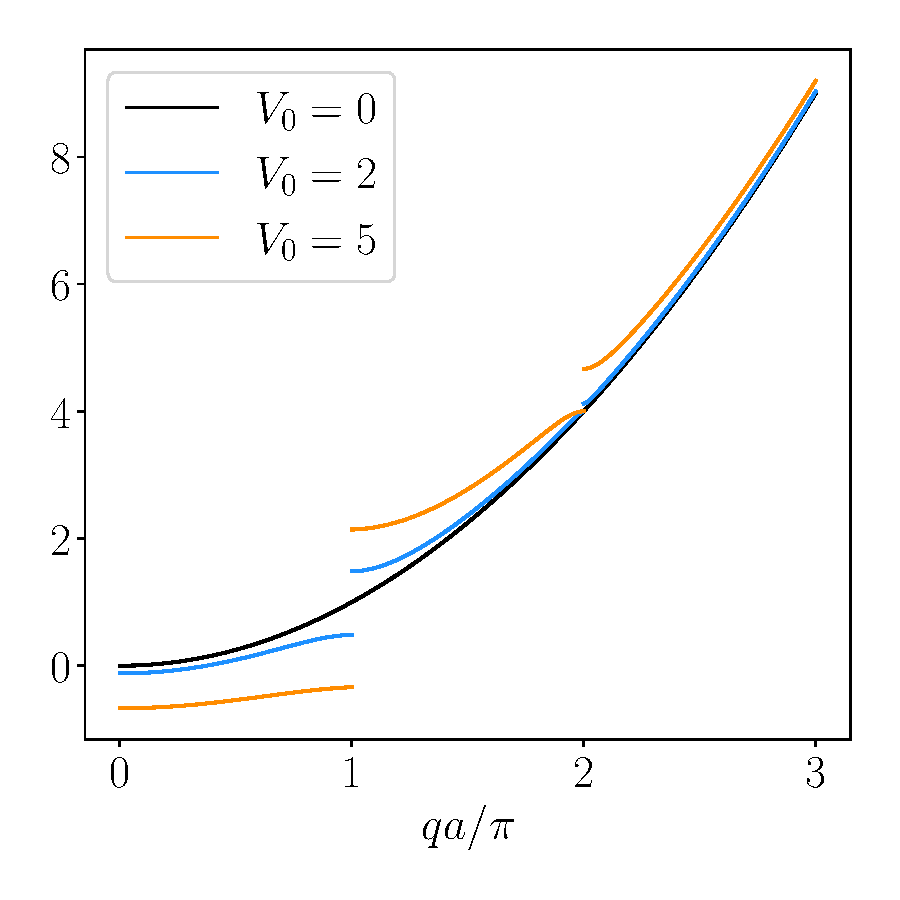
\includegraphics[width=0.66\textwidth]{img/unfolded.pdf}\label{fig:numerical-bands-unfolded}}
  \hfill
  \subfloat[Folded view]{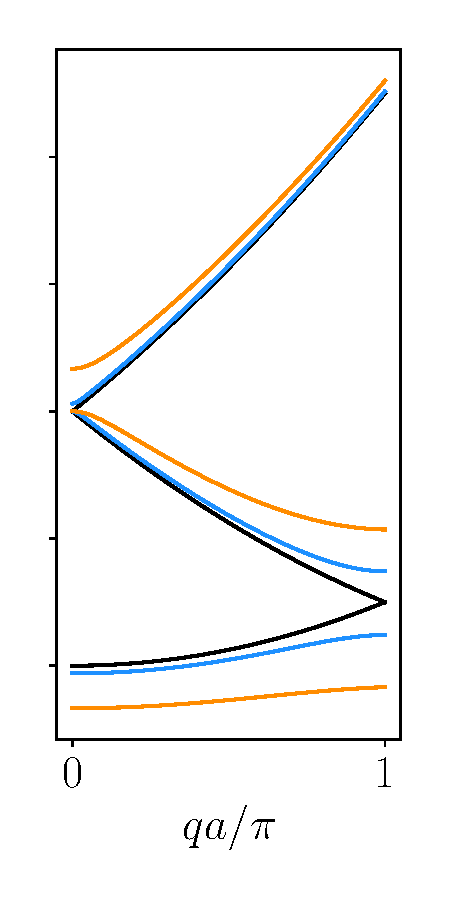
\includegraphics[width=0.33\textwidth]{img/folded.pdf}\label{fig:numerical-bands-folded}}
  \caption{\label{fig:numerical-bands} 
Numerical solution of Eq. \ref{eq:final-bands}, for different values of $V_0$. 
The curve for $V_0 = 0$ (black line) is the free-particle spectrum (a parabola in the momenta $q$). 
For $V_0\neq 0$ appear discontinuities in correspondence of $q=\pi/a, 2\pi/a, \dots$
The discontinuities are called \textbf{gaps}. We notice that the gaps get smaller as we increase the momenta: this is due to the increasing free particle energy, which becomes dominant, so the particle behaves like the lattice is not there.\\ \textit{That's when you can slide objects on top of tables and they don't get stuck!}\\
The subplot \textit{b} shows the same numerical result but folded in the first Brillouin zone. Indeed, due to the periodicity conditions to the solution to the Schrodinger equation, $\psi(q)$ would have the same value when shifting the momentum by $2\pi/a$. So a more convenient representation would not be the one in which $q$ ranges all real numbers, but the one which maps all momentums to the first Brillouin zone ($-\pi/a, \pi/a$) with shifts of $2\pi/a$. This is called \textbf{folding}. 
}
\end{figure}


\noindent \textbf{Take-away message}: When $V_0 \neq 0$ \textbf{the energies are compacted into bands} and there appear gaps.
A gap means that for those momenta there is not allowed state for the particle/atom/system.







\subsection{Tight-binding limit}

For large enough $V_0$ (larger than $E_R$). In this regime, we expect particles to be sufficiently localised in each well, but can also tunnel to the next well, jumping to the next minimum of the potential.

Instead of using the Block functions (the Bloch theorem solutions $\psi_{\alpha q}(x)$), we will use the harmonic oscillator solutions $\phi_\nu(x - x_n)$ to build a basis for the potential.

\begin{tcolorbox}[breakable, enhanced]
\begin{minipage}{0.45\textwidth}
\begin{center}
    $\psi_{\alpha q}(x)$

    $\alpha$ is the index of the band
\end{center}

    Ranging on all $\alpha$s and on all $q$s one has a complete set of wave-functions.
\end{minipage}\hfill
\begin{minipage}{0.45\textwidth}
\begin{center}
    $\phi_\nu(x - x_n)$

    $\nu$ harmonic energy level in the minimum $x_n$
\end{center}

    SPOILER: This does \textbf{not} form a basis!
\end{minipage}
\end{tcolorbox}



However, the harmonic oscillator wave-functions are not a basis. We can show that
$$\langle \phi_\nu (x-x_n) | \phi_\mu(x-x_n) \rangle = \delta_{\mu\nu}$$
so they behave like a basis for a single minima potential $x_n$.

But what if we fix $\nu$ and $\mu$, $\nu = \mu = 1$ for instance? The, the family of harmonic oscillator wave-functions in different wells ($x_n$ and $x_{n'}$) are not a basis. Indeed
$$\langle \phi_1 (x-x_n) | \phi_1(x-x_{n'}) \rangle
= \int dx \phi^*(x-x_n)\phi(x-x_{n'}) > 0 \qquad \text{for}\;\; n \neq n'$$
The last inequality comes from 
$\phi_1 (x-x_n) \propto e^{-x^2/\varepsilon^2} > 0$.
%
We conclude that \textbf{the family of harmonic oscillator wave-functions can be a good approximation, but they are not a perfect solution of the problem}\footnote{
    This is not a surprise... our potential is a cosine, the harmonic functions are just a mere approximation of it.}.
%
Instead, we want to find a basis, i.e. a set of functions solving the full problem or spanning the full space of wave-functions.\\


We already know the basis of Bloch functions $\psi_{\alpha q}(x)$. We now build a new basis from it performing a unitary transformation.\\

Let us define the \textbf{Wannier basis}, applying a Fourier transform on $\psi_{\alpha q}(x)$:
\begin{equation*}
w_\alpha(x-x_n) = \frac{1}{\sqrt{N_s}}
\sum_q e^{-iqx_n}\psi_{\alpha q}(x)
\end{equation*}
This is a valid transformation only for isolated bands. If the bands touch somewhere, then we have a degeneracy and it requires a particular treatment\footnote{
    There is a talk on YouTube (\href{https://www.youtube.com/watch?v=eHyqkB4ZMjw}{youtube.com/watch?v=eHyqkB4ZMjw}) by Giovanni Pizzi on this topic.
}.
%
One can prove that:
\begin{itemize}
\setlength\itemsep{1mm}
    \item $w_\alpha$ depends only on $x-x_n$
    \item $\langle w_\alpha(x-x_n) | w_\beta(x-x_{n'})\rangle = \delta_{\alpha\beta}\delta_{n n'}$, since the $u_q(x)$ are orthogonal
\end{itemize}

\noindent Our goal is to simplify the expression as much as possible, since there is the freedom
$$\psi_{\alpha q}(x) \longrightarrow \psi_{\alpha q}(x)e^{i\theta(q)}$$
because those functions
\begin{itemize}
\setlength\itemsep{1mm}
    \item are solutions to the same Schrodinger equations
    \item generate different set of Wannier $w_\alpha$
\end{itemize}


\noindent W. Kohn studied condensed matter and discovered (1959) that if $V(x)=V(-x)$ (inversion condition), then for each isolated $\alpha$ band $ \exists! w_\alpha(x-x_n)\;\; \forall n$ that is:
\begin{itemize}
\setlength\itemsep{1mm}
    \item real
    \item symmetric or anti-symmetric
    \item falling off exponentially with distance, i.e. $w_\alpha(x) \sim e^{-\hbar x^2}$ for large $x$
\end{itemize}

This result assures that there exist only one Wannier for each band which minimizes the $\psi$ at each site: there is no ambiguity in determining the Wannier basis! Furthermore, they are also exponentially localized, which allows us to do some simplification in the choice of the Wannier functions.

Instead of solving the problem using as many Wannier functions as you want (this is in principle the most general approach), under our assumptions, one can use just one or two of them. Indeed, since the Wannier functions are exponentially localized, one can associate them to a length scale. For a suitable choice, this length scale can be sufficiently small compared to the lattice periodicity.

Wannier states are orthogonal, but they are not eigenstates for the basis in which the Hamiltonian is written. The Hamiltonian elements in terms of the Wannier functions are
$$ - J_{j,j'}^{(\alpha,\beta)} \equiv \langle w_\alpha(x_j)|\hat{H}|w_\beta(x_{j'}) \rangle$$






% LECTURE 25 (19 jan)

\noindent Considering the lowest band, the related Wannier functions have $\alpha = 1$; therefore, let us define $\ket{j} = \ket{w_{\alpha=1}(x_j)}$. If and only if there is an appropriate energy separation ($T$, interactions $\ll$ gap), we can restrict the dynamics to the lowest band and write the hamiltonian as
\begin{equation}
\label{eq:tight-band-all}
    \Rightarrow \hat{H}_{TB} = -\sum_{j,\mu} J_{j,j+\mu}^{(1,1)} \left[ \ket{j}\bra{j+\mu} + h.c. \right]
\end{equation}
%
We can further simplify the expression: since $w(x_j)$ are exponentially localized, the overlap between functions is almost null if the functions are sufficiently separated $\Leftrightarrow \mu$ is sufficiently large.

\begin{center}
    \scalebox{1.4}{ 
\tikzset{every picture/.style={line width=0.75pt}} %set default line width to 0.75pt        

\begin{tikzpicture}[x=0.75pt,y=0.75pt,yscale=-1,xscale=1]
%uncomment if require: \path (0,100); %set diagram left start at 0, and has height of 100

%Shape: Wave [id:dp1124656768591269] 
\draw  [color={rgb, 255:red, 0; green, 0; blue, 0 }  ,draw opacity=1 ] (300.5,44.62) .. controls (295.11,30.13) and (289.97,16.32) .. (284,16.32) .. controls (278.02,16.32) and (272.88,30.13) .. (267.5,44.62) .. controls (262.11,59.12) and (256.97,72.92) .. (251,72.92) .. controls (245.02,72.92) and (239.88,59.12) .. (234.5,44.62) .. controls (229.11,30.13) and (223.97,16.32) .. (218,16.32) .. controls (212.02,16.32) and (206.88,30.13) .. (201.5,44.62) .. controls (196.11,59.12) and (190.97,72.92) .. (185,72.92) .. controls (179.02,72.92) and (173.88,59.12) .. (168.5,44.62) .. controls (163.11,30.13) and (157.97,16.32) .. (152,16.32) .. controls (146.02,16.32) and (140.88,30.13) .. (135.5,44.62) .. controls (130.11,59.12) and (124.97,72.92) .. (119,72.92) .. controls (113.02,72.92) and (107.88,59.12) .. (102.5,44.62) .. controls (97.11,30.13) and (91.97,16.32) .. (86,16.32) .. controls (80.02,16.32) and (74.88,30.13) .. (69.5,44.62) .. controls (64.11,59.12) and (58.97,72.92) .. (53,72.92) .. controls (47.02,72.92) and (41.88,59.12) .. (36.5,44.62) .. controls (31.11,30.13) and (25.97,16.32) .. (20,16.32) .. controls (16.1,16.32) and (12.55,22.2) .. (9.07,30.31) ;
%Curve Lines [id:da06441510036165143] 
\draw [color={rgb, 255:red, 255; green, 24; blue, 53 }  ,draw opacity=1 ]   (8,73) .. controls (38.29,73.02) and (37.91,50.51) .. (52.69,50.62) .. controls (67.46,50.73) and (68.69,73.02) .. (97.6,73) ;
%Curve Lines [id:da10660086824458115] 
\draw [color={rgb, 255:red, 0; green, 192; blue, 51 }  ,draw opacity=1 ]   (74,73) .. controls (104.29,73.02) and (103.91,50.51) .. (118.69,50.62) .. controls (133.46,50.73) and (134.69,73.02) .. (163.6,73) ;
%Curve Lines [id:da5007784416198438] 
\draw [color={rgb, 255:red, 0; green, 106; blue, 228 }  ,draw opacity=1 ]   (205.43,72.62) .. controls (235.72,72.64) and (235.34,50.13) .. (250.12,50.24) .. controls (264.89,50.34) and (266.12,72.64) .. (295.03,72.62) ;
%Shape: Ellipse [id:dp01210222813331252] 
\draw  [color={rgb, 255:red, 0; green, 0; blue, 0 }  ,draw opacity=0.44 ][line width=0.75]  (71.14,71.02) .. controls (71.14,65.64) and (77.78,61.29) .. (85.96,61.29) .. controls (94.15,61.29) and (100.78,65.64) .. (100.78,71.02) .. controls (100.78,76.39) and (94.15,80.75) .. (85.96,80.75) .. controls (77.78,80.75) and (71.14,76.39) .. (71.14,71.02) -- cycle ;

% Text Node
\draw (48.09,80.52) node [anchor=north west][inner sep=0.75pt]  [font=\scriptsize,color={rgb, 255:red, 255; green, 24; blue, 53 }  ,opacity=1 ]  {$j$};
% Text Node
\draw (106.89,80.32) node [anchor=north west][inner sep=0.75pt]  [font=\scriptsize,color={rgb, 255:red, 0; green, 192; blue, 51 }  ,opacity=1 ]  {$j+1$};
% Text Node
\draw (239.31,79.93) node [anchor=north west][inner sep=0.75pt]  [font=\scriptsize,color={rgb, 255:red, 0; green, 106; blue, 228 }  ,opacity=1 ]  {$j+\mu $};
% Text Node
\draw (26,7.22) node [anchor=north west][inner sep=0.75pt]  [font=\scriptsize]  {$V( x)$};


\end{tikzpicture}
 }
\end{center}

We remark that the Wannier functions are orthogonal, but there could be matrix elements outside the diagonal.
However, the dominant matrix elements will be the ones with largest overlap. For example, we can consider that $J_{j,j'} \gg J_{j,j+3}$ and then only small values of $\mu$ are taken into account for the case of $V_0 \gg E_R$.\\

If we take the Fourier transform, quantized over $jk$ and assuming periodic bound conditions,
\begin{equation}
\label{eq:tight-basis-def}
    \ket{k} = \frac{1}{\sqrt{N_s}}\sum_j e^{-ijka}\ket{j} \qquad\qquad \text{where}\;\; ja = \frac{2\pi}{N_s}n,\;\; n\in[0,N_s-1]
\end{equation}
%
\noindent It is easy to prove that $\{\ket{k}\}$ are an orthogonal set and that it is normalized to one: projecting on another Bloch wave-vector $\bra{q}$, $\Rightarrow$
\begin{align}
    \bra{q}\ket{k} &= \frac{1}{N_s} \sum_{j,j'} e^{ikqa}\bra{j}\ket{j'}e^{-ikj'a} 
    = \frac{1}{N_s} \sum_{j,j'} \delta_{j,j'} e^{ikja}e^{-iqj'a}
    = \frac{1}{N_s} \sum_j e^{i(k-q)ja}\nonumber\\
    &= \frac{1}{N_s}
    \begin{cases}
        N_s& \text{if}\; k=q\\
        0 &\text{else}  \qquad \longleftarrow \text{all the momenta are out of phase}
    \end{cases}
    \label{eq:phase-sum}
\end{align}



The hamiltonian \ref{eq:tight-band-all} can be rewritten in the momentum space as
\begin{equation}
\label{eq:tight-band-momentum}
    \hat{H}_{TB} = -\sum_{j,\mu} J_{j,j+\mu}\left( \ket{j}\bra{j+\mu} + h.c. \right)
\end{equation}
Remember that this expression is considering only the lowest energy band. We want to study its spectrum, which means to diagonalize the hamiltonian.

First, we notice that the Wannier functions are real (in a suitable gauge), so all of the hamiltonian matrix elements are real numbers.

\noindent Second, because all lattice sites are physically equivalent, we consider the translational symmetry to consider the $J$ as functions of $\mu$ only:
\begin{equation*}
    J_{j.j+\mu} \equiv J_\mu \qquad (\in \mathcal{R}) \;.
\end{equation*}

\noindent We now can diagonalize the hamiltonian


\begin{align*}
    \Longrightarrow \hat{H}_{TB} &\overset{\ref{eq:tight-band-momentum}}{=} -\sum_{j,\mu} J_{j.j+\mu}
    \left( \ket{j}\bra{j+\mu} + h.c. \right)
        \overset{\text{\ref{eq:tight-basis-def}}}{=}\\
    &= -\sum_{j,\mu} \frac{1}{N_s}\sum_k\sum_q  J_\mu e^{+i(j)ka} e^{-i(j+\mu)qa} \ket{k}\bra{q} + h.c. = \\
    &= - \frac{1}{N_s}\sum_{\mu,k,q}
        J_\mu \underbrace{\sum_{j} e^{ija(k-q)}}_{=\delta_{k,q}\cdot N_s \;\; \text{(\ref{eq:phase-sum})}} e^{-i\mu qa} \ket{k}\bra{q} + h.c. =\\
    &= -\sum_\mu\sum_k J_\mu
        \left( e^{-ik\mu a} \ket{k}\bra{k} + e^{ik\mu a} \ket{k}\bra{k} \right) =\\
    &= -\sum_{k,\mu} J_\mu \cdot 2\cos(\mu ka) \ket{k}\bra{k} \equiv \sum_k E(k) \ket{k}\bra{k}
\end{align*}
but we care only about the spectrum (eigenvalues):
\begin{equation}
\label{eq:spectrum-tight-binding}
    E(k) = -2\sum_\mu J_\mu \cos{(\mu ka)}
\end{equation}

In the tight-binding limit, we can neglect higher values of $\mu$. For example, we set $J_\mu = 0$, say, for $\mu > 2$; then $E(k) \simeq -2J_1 \cos{(ka)} -2J_2 \cos{(2ka)}$.
%
We can be more severe and ignore $J_\mu$ for $\mu > 1$, because $J_1 \gg J_2 \gg J_3 \gg \dots$ by orders of magnitude due to the exponential localization of Wannier functions. Doing this, the spectrum is completely determined by $J_1$ itself

\begin{minipage}{0.50\textwidth}
    \begin{center}
    \scalebox{0.95}{ 

\tikzset{every picture/.style={line width=0.75pt}} %set default line width to 0.75pt        

\begin{tikzpicture}[x=0.75pt,y=0.75pt,yscale=-1,xscale=1]
%uncomment if require: \path (0,175); %set diagram left start at 0, and has height of 175

%Straight Lines [id:da4301961974434454] 
\draw    (140,169.21) -- (140,12.2) ;
\draw [shift={(140,10.2)}, rotate = 90] [color={rgb, 255:red, 0; green, 0; blue, 0 }  ][line width=0.75]    (6.56,-1.97) .. controls (4.17,-0.84) and (1.99,-0.18) .. (0,0) .. controls (1.99,0.18) and (4.17,0.84) .. (6.56,1.97)   ;
%Straight Lines [id:da644600047896886] 
\draw    (10.5,98.86) -- (266.57,98.86) ;
\draw [shift={(268.57,98.86)}, rotate = 180] [color={rgb, 255:red, 0; green, 0; blue, 0 }  ][line width=0.75]    (6.56,-1.97) .. controls (4.17,-0.84) and (1.99,-0.18) .. (0,0) .. controls (1.99,0.18) and (4.17,0.84) .. (6.56,1.97)   ;
%Shape: Wave [id:dp8332830628724615] 
\draw  [color={rgb, 255:red, 255; green, 21; blue, 21 }  ,draw opacity=1 ] (40,43.14) .. controls (58.1,43.14) and (73.69,69.97) .. (90,98.14) .. controls (106.31,126.32) and (121.9,153.14) .. (140,153.14) .. controls (158.1,153.14) and (173.69,126.32) .. (190,98.14) .. controls (206.31,69.97) and (221.9,43.14) .. (240,43.14) ;
%Shape: Rectangle [id:dp8283156136322417] 
\draw  [color={rgb, 255:red, 0; green, 0; blue, 0 }  ,draw opacity=0.45 ][dash pattern={on 4.5pt off 4.5pt}] (40,43.1) -- (240,43.1) -- (240,153.1) -- (40,153.1) -- cycle ;

% Text Node
\draw (275,91.83) node [anchor=north west][inner sep=0.75pt]  [font=\normalsize]  {$k$};
% Text Node
\draw (146.79,5.69) node [anchor=north west][inner sep=0.75pt]  [font=\normalsize]  {$E$};
% Text Node
\draw (17.71,102.83) node [anchor=north west][inner sep=0.75pt]  [font=\scriptsize]  {$-\frac{\pi }{a}$};
% Text Node
\draw (242,101.4) node [anchor=north west][inner sep=0.75pt]  [font=\scriptsize]  {$+\frac{\pi }{a}$};
% Text Node
\draw (120.29,27.4) node [anchor=north west][inner sep=0.75pt]  [font=\scriptsize]  {$2J_{1}$};
% Text Node
\draw (113.14,156.26) node [anchor=north west][inner sep=0.75pt]  [font=\scriptsize]  {$-2J_{1}$};


\end{tikzpicture}
 }
    \end{center}
\end{minipage}\hfill
\begin{minipage}{0.40\textwidth}
    and the bandwidth is
    \begin{align*}
        \Delta E &= E\left(k=\frac{\pi}{a}\right) - E\left(k=0\right)\\
        &= 2J_1 - (- 2J_1) = 4J_1
    \end{align*}
\end{minipage}


\begin{tcolorbox}[breakable, enhanced]
\textbf{Recap}\\

In the tight-binding limit, the potential is sufficiently deep and the bands are sufficiently separated. Under these circumstances, the lattice is able to confine the wave-function to a single site. The lowest band of an atom in a lattice is described by the (nearest-neighbor) hamiltonian
\begin{equation*}
    \hat{H}_{TB} = -J\sum_j
    \left( \ket{j}\bra{j+1} + \ket{j+1}\bra{j}\right)
\end{equation*}

The amplitude of the hopping (or tunneling) process is basically $J\simeq J_1$. The transmission is not exactly like the problem you have seen in an introductory course on Quantum Mechanics, but it is really similar.

\begin{center}
    \scalebox{1.2}{ 

\tikzset{every picture/.style={line width=0.75pt}} %set default line width to 0.75pt        

\begin{tikzpicture}[x=0.75pt,y=0.75pt,yscale=-1,xscale=1]
%uncomment if require: \path (0,100); %set diagram left start at 0, and has height of 100

%Straight Lines [id:da8895757852919295] 
\draw [color={rgb, 255:red, 255; green, 120; blue, 0 }  ,draw opacity=1 ][line width=1.5]    (112.4,62.85) -- (130.8,62.85) ;
%Straight Lines [id:da6552386630403477] 
\draw [color={rgb, 255:red, 255; green, 120; blue, 0 }  ,draw opacity=1 ][line width=1.5]    (178.15,62.9) -- (196.55,62.9) ;
%Straight Lines [id:da7235324665708592] 
\draw [color={rgb, 255:red, 255; green, 120; blue, 0 }  ,draw opacity=1 ][line width=1.5]    (46.15,62.9) -- (64.55,62.9) ;
%Shape: Wave [id:dp2133679410198479] 
\draw  [color={rgb, 255:red, 0; green, 0; blue, 0 }  ,draw opacity=1 ] (232.8,34.21) .. controls (228.79,24.15) and (224.76,16.32) .. (220.26,16.32) .. controls (214.29,16.32) and (209.14,30.13) .. (203.76,44.62) .. controls (198.38,59.12) and (193.23,72.92) .. (187.26,72.92) .. controls (181.29,72.92) and (176.14,59.12) .. (170.76,44.62) .. controls (165.38,30.13) and (160.23,16.32) .. (154.26,16.32) .. controls (148.29,16.32) and (143.14,30.13) .. (137.76,44.62) .. controls (132.38,59.12) and (127.23,72.92) .. (121.26,72.92) .. controls (115.29,72.92) and (110.14,59.12) .. (104.76,44.62) .. controls (99.38,30.13) and (94.23,16.32) .. (88.26,16.32) .. controls (82.29,16.32) and (77.14,30.13) .. (71.76,44.62) .. controls (66.38,59.12) and (61.23,72.92) .. (55.26,72.92) .. controls (49.29,72.92) and (44.14,59.12) .. (38.76,44.62) .. controls (33.38,30.13) and (28.23,16.32) .. (22.26,16.32) .. controls (17.52,16.32) and (13.3,25.02) .. (9.07,35.86) ;
%Shape: Circle [id:dp489370128374481] 
\draw  [draw opacity=0][fill={rgb, 255:red, 0; green, 98; blue, 230 }  ,fill opacity=1 ] (116,62.98) .. controls (116,60.12) and (118.32,57.8) .. (121.18,57.8) .. controls (124.04,57.8) and (126.35,60.12) .. (126.35,62.98) .. controls (126.35,65.84) and (124.04,68.15) .. (121.18,68.15) .. controls (118.32,68.15) and (116,65.84) .. (116,62.98) -- cycle ;
%Shape: Arc [id:dp6949731840439705] 
\draw  [draw opacity=0] (130.17,50.2) .. controls (136.44,48.03) and (144.13,46.75) .. (152.44,46.75) .. controls (165.67,46.75) and (177.32,49.99) .. (184.18,54.91) -- (152.44,65.13) -- cycle ; \draw [color={rgb, 255:red, 71; green, 156; blue, 255 }  ,draw opacity=1 ]   (130.17,50.2) .. controls (136.44,48.03) and (144.13,46.75) .. (152.44,46.75) .. controls (164.21,46.75) and (174.74,49.32) .. (181.74,53.35) ; \draw [shift={(184.18,54.91)}, rotate = 207.8] [fill={rgb, 255:red, 71; green, 156; blue, 255 }  ,fill opacity=1 ][line width=0.08]  [draw opacity=0] (5.36,-2.57) -- (0,0) -- (5.36,2.57) -- (3.56,0) -- cycle    ; 
%Shape: Arc [id:dp7943300133194532] 
\draw  [draw opacity=0] (112.65,50) .. controls (106.55,47.89) and (99.08,46.65) .. (91,46.65) .. controls (78.14,46.65) and (66.81,49.79) .. (60.14,54.57) -- (91,64.51) -- cycle ; \draw [color={rgb, 255:red, 71; green, 156; blue, 255 }  ,draw opacity=1 ]   (112.65,50) .. controls (106.55,47.89) and (99.08,46.65) .. (91,46.65) .. controls (79.62,46.65) and (69.43,49.11) .. (62.62,52.99) ; \draw [shift={(60.14,54.57)}, rotate = 332.42] [fill={rgb, 255:red, 71; green, 156; blue, 255 }  ,fill opacity=1 ][line width=0.08]  [draw opacity=0] (5.36,-2.57) -- (0,0) -- (5.36,2.57) -- (3.56,0) -- cycle    ; 

% Text Node
\draw (116.29,78.12) node [anchor=north west][inner sep=0.75pt]  [font=\small,color={rgb, 255:red, 255; green, 120; blue, 0 }  ,opacity=1 ]  {$j$};
% Text Node
\draw (173.09,77.92) node [anchor=north west][inner sep=0.75pt]  [font=\small,color={rgb, 255:red, 255; green, 120; blue, 0 }  ,opacity=1 ]  {$j+1$};
% Text Node
\draw (40.91,77.93) node [anchor=north west][inner sep=0.75pt]  [font=\small,color={rgb, 255:red, 255; green, 120; blue, 0 }  ,opacity=1 ]  {$j-1$};
% Text Node
\draw (2.8,40.42) node [anchor=north west][inner sep=0.75pt]  [font=\footnotesize]  {$V( x)$};


\end{tikzpicture}
 }
\end{center}

\end{tcolorbox}


The latest developments allow us to answer to this question: how does a single particle behave on a lattice? The behavior of many (interacting) particles will be a topic of discussion only after we answer to the first question.




\section{Quantum walk or Brownian motion of a single particle}

A lattice with only one particle is, in practice, an analog simulation of the Brownian motion.
The particle can tunnel from $j$ either to $j+1$ or $j-1$, or even a superposition of the two. We wish to predict the location of the particle after some time steps.
%
We assume that the particle is in site $j$ at $t=0$ $$\ket{\psi(0)} = \ket{0}\otimes\ket{0}\otimes...\otimes \ket{0}\otimes\underbrace{\ket{1}}_{j}\otimes\ket{0} \otimes ... = \ket{0...010...} \;\;.$$
and we want to compute its evolution
$$\ket{\psi(t)} = e^{-i\hat{H}t/\hbar}\ket{\psi(0)} \qquad \text{where}\qquad \hat{H} = -2J\sum_k\cos(ka)\ket{k}\bra{k} \;\;.$$
%
The evolution is simple to compute in the momentum space:
\begin{align*}
    \ket{\psi(t)} &= \frac{1}{\sqrt{N_s}} \sum_k e^{-i\hat{H}t/\hbar} e^{ikja} \ket{k} = \\
    &= \frac{1}{\sqrt{N_s}} \sum_k e^{ikja} e^{-iE(k)t/\hbar} \ket{k}
    = \frac{1}{\sqrt{N_s}} \sum_k e^{ikja} e^{-i2J\cos(ka)t/\hbar} \ket{k} \overset{\text{\ref{eq:tight-basis-def}}}{=}\\ % back to wannier, then anti-transform
    &= \frac{1}{\sqrt{N_s}} \sum_{k,j'} e^{ikja} e^{-i2J\cos(ka)t/\hbar} e^{-ikj'a} \ket{j'}
\end{align*}

\noindent Let $\ket{\psi(t)} = \sum_{j'} c_{j'}(t)\ket{j'}$; the coefficients $c_{j'}(t)$ can be used to express the probabilities of finding an atom in $j'$ if it is initially in site $j$:
\begin{equation*}
    P_{j'}(t) = |c_{j'}(t)|^2
    \qquad:\qquad
    c_{j'}(t) \equiv \sum_k \frac{1}{\sqrt{N_s}} e^{ik(j-j')a} e^{-i2J\cos(ka)t/\hbar}
\end{equation*}
author new line
Now we want to write the coefficients in terms of (Hansen-)Bessel functions:
\begin{equation*}
    I_n (x) = \frac{1}{2\pi} \int_{-\pi}^{\pi} dz \; e^{inz} e^{-ix\sin(z)} \;\;.
\end{equation*}

\noindent In this case there is a simple trick, which is to reshape the coefficients expression at the limit $N_s\rightarrow\infty$. Indeed, one can rewrite the coefficients as a Riemann sum and go to the infinity limit, as we have previously done for the thermodynamics of photons. In particular
\begin{equation*}
    \frac{1}{N_s}\sum_k \;\;\text{with}\;\; ka=\frac{2\pi}{N_s}n
    \qquad\xrightarrow{N_s\rightarrow\infty}\qquad
    \frac{1}{2\pi}\int_0^{2\pi} d(ka) 
\end{equation*}
\begin{align*}
    \Longrightarrow\qquad
    c_{j'}(t) &=\frac{1}{2\pi} \int_{0}^{2\pi} d(ka) e^{i(j-j')ka} e^{-i2J\cos(ka)t/\hbar} \equalexpl{$v=ka-\pi$} \\
    &= \frac{1}{2\pi} \int_{-\pi}^{\pi} dv\; 
        e^{i\pi(j-j')} e^{i(j-j')v} e^{i\frac{2Jt}{\hbar}\sin(v)}
        \cdot \underbrace{\text{(phase factor)}}_{\text{not very rigorous...}}
\end{align*}

We have not been very rigorous in the last passage. We see that the change of variable is not able to return a $\sin(v)$ in the exponential. The change of variable $v=ka-\pi/2$ would be more appropriate to make the $\sin$ appear, but the integral boundaries would be $[3\pi/2,-\pi/2]$. Nevertheless, the result would numerically be the same, because the integral arguments are periodic and the integration interval still covers an entire period of the arguments.

The conclusion is that $c_{j'}$ is proportional (same module, but different phase) to the Bessel functions of $2Jt/\hbar$:
\begin{equation*}
    c_{j'} \sim I_{j,j'} \left( \frac{2Jt}{\hbar} \right)
\end{equation*}

\noindent We can plot them and describe some interesting behavior:

\begin{minipage}{0.50\textwidth}
\scalebox{1.0}{ 

\tikzset{every picture/.style={line width=0.75pt}} %set default line width to 0.75pt        

\begin{tikzpicture}[x=0.75pt,y=0.75pt,yscale=-1,xscale=1]
%uncomment if require: \path (0,130); %set diagram left start at 0, and has height of 130

%Straight Lines [id:da42292147954355674] 
\draw    (23,121) -- (23,11) ;
\draw [shift={(23,9)}, rotate = 90] [color={rgb, 255:red, 0; green, 0; blue, 0 }  ][line width=0.75]    (7.65,-2.3) .. controls (4.86,-0.97) and (2.31,-0.21) .. (0,0) .. controls (2.31,0.21) and (4.86,0.98) .. (7.65,2.3)   ;
%Straight Lines [id:da0938116227302922] 
\draw    (7.5,102) -- (239.25,102) ;
\draw [shift={(241.25,102)}, rotate = 180] [color={rgb, 255:red, 0; green, 0; blue, 0 }  ][line width=0.75]    (7.65,-2.3) .. controls (4.86,-0.97) and (2.31,-0.21) .. (0,0) .. controls (2.31,0.21) and (4.86,0.98) .. (7.65,2.3)   ;
%Curve Lines [id:da7388142079293656] 
\draw [color={rgb, 255:red, 255; green, 26; blue, 26 }  ,draw opacity=1 ]   (23.58,31) .. controls (45.58,30.5) and (67.08,124) .. (96.58,124.5) .. controls (126.08,125) and (140.08,84) .. (161.08,84) .. controls (182.08,84) and (202,135.83) .. (231.5,108.33) ;
%Curve Lines [id:da2797400644106053] 
\draw [color={rgb, 255:red, 25; green, 108; blue, 201 }  ,draw opacity=1 ]   (23.25,101.5) .. controls (73.75,43) and (119.33,117.67) .. (144.25,118) .. controls (169.17,118.33) and (183.5,94.67) .. (193.5,90.67) ;
%Curve Lines [id:da34662757016201506] 
\draw [color={rgb, 255:red, 163; green, 0; blue, 143 }  ,draw opacity=1 ]   (23.25,101.5) .. controls (76.83,73.67) and (83.83,106.67) .. (110.5,109) .. controls (137.17,111.33) and (139.83,103) .. (153.5,94.67) ;
%Shape: Circle [id:dp028498302535310938] 
\draw  [color={rgb, 255:red, 0; green, 196; blue, 69 }  ,draw opacity=1 ][line width=0.75]  (67,101.67) .. controls (67,99.83) and (68.49,98.33) .. (70.33,98.33) .. controls (72.17,98.33) and (73.67,99.83) .. (73.67,101.67) .. controls (73.67,103.51) and (72.17,105) .. (70.33,105) .. controls (68.49,105) and (67,103.51) .. (67,101.67) -- cycle ;
%Shape: Circle [id:dp30028872852521227] 
\draw  [color={rgb, 255:red, 0; green, 196; blue, 69 }  ,draw opacity=1 ][line width=0.75]  (131,101.67) .. controls (131,99.83) and (132.49,98.33) .. (134.33,98.33) .. controls (136.17,98.33) and (137.67,99.83) .. (137.67,101.67) .. controls (137.67,103.51) and (136.17,105) .. (134.33,105) .. controls (132.49,105) and (131,103.51) .. (131,101.67) -- cycle ;
%Shape: Circle [id:dp6051192164240733] 
\draw  [color={rgb, 255:red, 0; green, 196; blue, 69 }  ,draw opacity=1 ][line width=0.75]  (184,101.67) .. controls (184,99.83) and (185.49,98.33) .. (187.33,98.33) .. controls (189.17,98.33) and (190.67,99.83) .. (190.67,101.67) .. controls (190.67,103.51) and (189.17,105) .. (187.33,105) .. controls (185.49,105) and (184,103.51) .. (184,101.67) -- cycle ;
%Shape: Square [id:dp9109798777185496] 
\draw  [draw opacity=0][fill={rgb, 255:red, 255; green, 26; blue, 26 }  ,fill opacity=1 ] (102,20.33) -- (110.17,20.33) -- (110.17,28.5) -- (102,28.5) -- cycle ;
%Shape: Square [id:dp708254493093753] 
\draw  [draw opacity=0][fill={rgb, 255:red, 25; green, 108; blue, 201 }  ,fill opacity=1 ] (102.33,40.33) -- (110.5,40.33) -- (110.5,48.5) -- (102.33,48.5) -- cycle ;
%Shape: Square [id:dp732226894539835] 
\draw  [draw opacity=0][fill={rgb, 255:red, 163; green, 0; blue, 143 }  ,fill opacity=1 ] (102.67,60.33) -- (110.83,60.33) -- (110.83,68.5) -- (102.67,68.5) -- cycle ;

% Text Node
\draw (4.5,2.4) node [anchor=north west][inner sep=0.75pt]  [font=\small]  {$c_{j}$};
% Text Node
\draw (11.5,24.9) node [anchor=north west][inner sep=0.75pt]  [font=\scriptsize]  {$1$};
% Text Node
\draw (115.33,18.73) node [anchor=north west][inner sep=0.75pt]  [font=\scriptsize]  {$j'=j\ \ \ \ \ \ \ \ \ \Rightarrow \ J_{0}$};
% Text Node
\draw (115,38.73) node [anchor=north west][inner sep=0.75pt]  [font=\scriptsize]  {$j'=j\pm 1\ \ \ \Rightarrow \ J_{1} \ \text{or} \ \ J_{-1}$};
% Text Node
\draw (115.33,58.73) node [anchor=north west][inner sep=0.75pt]  [font=\scriptsize]  {$j'=j\pm 2\ \ \ \Rightarrow \ J_{2} \ \text{or} \ \ J_{-2}$};
% Text Node
\draw (243,85.4) node [anchor=north west][inner sep=0.75pt]  [font=\small]  {$t$};


\end{tikzpicture}
 }
\end{minipage}\hfill
\begin{minipage}{0.45\textwidth}
\begin{itemize}
    \item $c_{j}$ starts from $1$ (we prepared the system in this state) and then the particle starts spreading.
    \item For some time $t^*$ there exist null points of $c_j(t^*) = 0$. This is a destructive interference, nothing less than diffraction. This is why we can reproduce the same physics with purely optical systems.
\end{itemize}
\end{minipage}



\vspace{1em}

This concludes our discussion about single particle physics. Now we are ready to approach this topic from a many body perspective, i.e. many interacting atoms in a lattice.





\section{Interactions}

Materials are made by many interacting particles. For example, the interaction between electrons leads to superconductivity, ferromagnetism or insulators. These topics are usually studied in quantum many-body courses.

The simulations of many body systems are computationally challenging, because the dimension of the Hilbert spaces scales exponentially in the system size. For instance, a chain of $N_s$ spins implies that $dim(H_s) = 2^{N_s}$.\\

It is, at least computationally, an intractable problem. That is why most of the 20th century condenser matter physics has been devoted to develop methods, theoretical and (later) numerical, to address this problems, aiming to simplify the dimensionality of the problem.
\textbf{Analog quantum simulations} allow us to tackle the problem from another point of view, which is to deal with an target exponentially large Hilbert space using a system which is itself an exponentially large Hilbert space.
Analog quantum simulations are basically a mapping of a target problem to a real physical system.\\

\noindent This is a sufficient motivation to describe briefly the interactions and what kind of phenomena we can observe and model using algebraic models.

\vspace{1em}

Let us consider two atoms as dipoles (this is a rather classical way to solve the problem, since we know that atoms cannot have a permanent dipole).
The interaction potential between them is
\begin{equation*}
    V(\underbrace{\vec{r}_1-\vec{r}_2}_{\equiv\vec{r}}) = \frac{1}{4\pi\varepsilon_0r^3}
    \left[ \vec{d}_1\cdot \vec{d}_2 -3(\vec{d}_1\cdot\vec{r})(\vec{d}_2\cdot\vec{r})\right]
\end{equation*}

The scattering potential is complicated to solve, but for low $T$ (low energy) only the angular momentum $L=0$ is relevant (the centrifugal barrier inhibits the atom to scatter to larger angular momentum states). The angular momentum $\vec{L}$ is intended with respect to the relative coordinate $\vec{r}$.


\subsection{S-wave channel/scattering}

$L=0$ is usually called \textbf{S-wave channel} or scattering. It means basically that 
$$V(\vec{r}) \simeq u_0\delta^{(3)}(\vec{r}) \;\;.$$
Thinking of atoms as spheres, this approximation means that there is interaction only when the spheres overlap completely. We know it is not true, because there is a potential barrier that forbids the atoms to do so... instead, the atoms would ``touch" when their relative distance is some value $r^*>0$ (an ``effective bouncing radius").

Nevertheless, there exist some atoms that overlap, and they are bosonic atoms, like $\prescript{87}{}{Rb}$, $\prescript{27}{}{Na}$ and $\prescript{7}{}{Li}$.

We observe that combinations of an even number of fermions lead to bosonic wave-functions (spins would sum up to integer values $\Rightarrow$ Boson statistics).

In neutral atoms, the number of protons (it is made of three quarks, so it is a fermion) equals to the number of electrons. The number of fermions is even. The only way to discriminate is to count neutrons!

\noindent \textbf{Example} of Lithium: $Z_{Li} = 3$.
\begin{align*}
    \text{Neutrons}(\prescript{7}{}{Li}) = 7-Z_{Li} = 4 &\qquad \text{(even)} &\Rightarrow \text{boson}&&\\
    \text{Neutrons}(\prescript{6}{}{Li}) = 6-Z_{Li} = 3 &\qquad \text{(odd)} &\Rightarrow \text{fermion}&&
\end{align*}

\noindent What does this mean in terms of S-wave?
\begin{itemize}
    \item \textbf{Fermions} interact with S-Wave if the two atoms are in different internal states.
    \begin{equation*}
        (n_1, l_1, m_1, s_1)
        \neq (n_2, l_2, m_2, s_2)
    \end{equation*}
    Examples: $\prescript{6}{}{Li}$, $\prescript{40}{}{K}$, ...
    \item It is easier to describe \textbf{bosons}.

    We take the state $\psi_a(x)$ where $\alpha$ is a collection of quantum numbers $\alpha = (n, l, m)$ or another level of lattice physics (for example a Wannier function). The (most generic) wave-function of two atoms is symmetric for exchange of $r_i$:
    \begin{equation*}
        \Psi_{\alpha\beta}(\vec{r}_1,\vec{r}_2) = \frac{1}{2}
        \left[
            \psi_\alpha(\vec{r}_1)\psi_\beta(\vec{r}_2) +
            \psi_\alpha(\vec{r}_2)\psi_\beta(\vec{r}_1)
        \right]\delta_{\alpha\beta}
    \end{equation*}
    You may also have seen this in terms of the Slater determinant.
    
    The internal energy would be
    \begin{align*}
        E_{int} &= \int d\vec{r}_1 d\vec{r}_2
        \Psi^*(\vec{r}_1,\vec{r}_2) u_0 \delta(\vec{r}_1-\vec{r}_2) \Psi(\vec{r}_1,\vec{r}_2)\\
        % all the possibilities
        &= \frac{u_0}{4} \int d\vec{r}_1 d\vec{r}_2
        \left[
            \psi(\vec{r}_1)\psi(\vec{r}_2)\psi(\vec{r}_1)\psi(\vec{r}_2) + ... + \psi(\vec{r}_2)\psi(\vec{r}_1)\psi(\vec{r}_2)\psi(\vec{r}_1)
        \right] \delta(\vec{r}_1 - \vec{r}_2)\\
        &= \frac{u_0}{4} \int d\vec{r}_1 d\vec{r}_2 \cdot
            4 |\psi(\vec{r}_1)|^2|\psi(\vec{r}_2)|^2
            \delta(\vec{r}_1 - \vec{r}_2)\\
        &= u_0 \int d\vec{r}_1 |\psi(\vec{r}_1)|^4 =
            u_0 \int dr |\psi(r)|^4 \equiv U
    \end{align*}
    
    Thus, if we know the wave-functions then we know the energy of interaction. If we had Wannier functions, we could also write
    \begin{equation*}
    \Rightarrow \bra{w(x_j)w(x_{j'})} \hat{V}_{int} \ket{w(x_j)w(x_{j'})} = \delta_{j,j'}U
    \end{equation*}


\end{itemize}







% LECTURE 26 (20 jan)

\section{Quantum phase transitions}

In this section we will review two models featuring quantum phase transitions, with a particular focus on a quantum phase transition from superfluid to Mott insulator observed with ultra-cold atoms\footnote{\href{https://www.nature.com/articles/415039aa}{Greiner, M., Mandel, O., Esslinger, T. et al. Quantum phase transition from a superfluid to a Mott insulator in a gas of ultracold atoms - Nature 415, 39–44 (2002)}}.





\subsection{Bose-Hubbard model}

Let us consider a system of $N$ bosons hopping on a $N_s$ sites lattice (with hopping parameter $J$) and interacting when close enough.

We need some more formalism to address this problem properly. To take a shortcut, we just say that, like for photons, the Wannier functions $\ket{j}\equiv\ket{w_j}$ can be written in terms of creation/destruction operators (satisfying the harmonic oscillator commutation rules)
$$ \left[\hat{a}_j, \hat{a}_{j'}^\dag\right] = \delta_{j,j'}
   \qquad
   \left[\hat{a}_j, \hat{a}_{j'}\right] =
   \left[\hat{a}_j, \hat{a}_{j'}^\dag\right] = 0
$$
which create/destroy bosons in a Wannier function mode. Every particle is a quantum field! Thus, the hopping Hamiltonian can be rewritten as
\begin{align*}
\hat{H}_{hop} &= -J\sum_j
    \left( \ket{j+1}\bra{j} + h.c. \right) =\\
&= -J\sum_j
    \left( \hat{a}_{j+1}^\dag\hat{a}_{j} + \hat{a}_{j}^\dag\hat{a}_{j+1} \right)
\end{align*}

Now we want to write the interaction part $\hat{H}_{\text{int}}$. Also in this case, the Hilbert space is similar to the one with photons on mode $j$. Instead of counting photons, we count the number of bosons in each mode (Wannier function) $\ket{w_j}$:
\begin{equation*}
    \ket{n_{j=1}} \otimes \ket{n_{j=2}} \otimes ... \otimes \ket{n_{j=1}} \otimes ...
\end{equation*}
We have previously seen that the energy of two atoms in the same orbital is $U$. Now we want to find an hamiltonian that returns $U$ when it is contracted with a state with two particles in the same mode, and return zero for states with just one particle.

We do not prove it in a rigorous way, but we will see that the following hamiltonian  satisfies our requests
\begin{equation*}
    \hat{H}_{int} = \frac{U}{2}\sum_j \hat{n}_j (\hat{n}_j-1)  \qquad\qquad \text{where }\;\; \hat{n}_j = \hat{a}_j^\dag \hat{a}_j
\end{equation*}

\noindent Let us check the quantity $\bra{\psi}\hat{H}_{int}\ket{\psi}$ for...
\begin{itemize}
    \item ...\emph{2 particles}: $\ket{\psi} = \ket{0}\otimes ...\otimes\ket{0}\otimes\ket{2_j}\otimes\ket{0}\otimes ...$\\
    $$\begin{cases}
        \hat{H}_{int}^{(j)} \ket{0_j} = \frac{U}{2}0(0-1)\ket{0_j} = 0\ket{0_j}\\
        \hat{H}_{int}^{(j)} \ket{2_j} = \frac{U}{2}2(2-1)\ket{2_j} = U\ket{2_j}
    \end{cases} \Rightarrow \bra{\psi}\hat{H}_{int}\ket{\psi} = U = E_{int}$$
    \item ...\emph{1 particle}: $\ket{\psi} = \ket{0}\otimes ...\otimes\ket{0}\otimes\ket{1_j}\otimes\ket{0}\otimes ...$\\
    \begin{equation}
    \label{eq:bh-interaction-min}
    \begin{cases}
        \hat{H}_{int}^{(j)} \ket{0_j} = \frac{U}{2}0(0-1) \ket{0_j} = 0\ket{0_j}\\
        \hat{H}_{int}^{(j)} \ket{2_j} = \frac{U}{2}1(1-1) \ket{2_j} = 0\ket{1_j}
    \end{cases}
    \Rightarrow  \bra{\psi}\hat{H}_{int}\ket{\psi} = 0
    \end{equation}\\
    The interaction energy is zero because one particle is not interacting with any other one.
\end{itemize}


The total hamiltonian for the Bose-Hubbard model is
\begin{equation}
    \hat{H} = -J\sum_j\left(
        \hat{a}_{j+1}^\dag\hat{a}_{j} + \hat{a}_{j}^\dag\hat{a}_{j+1}
    \right) + \frac{U}{2} \sum_j \hat{n}_{j}(\hat{n}_{j}-1)
\end{equation}
%
The problem is that the basis we have chosen do not diagonalize both terms at the same time: $\left[\hat{H}_{hop}, \hat{H}_{int}\right] \neq 0$. Diagonalize $\hat{H}$ is hard: in principle there could be a basis, but no one has found it so far. There is no exact numerical solution either. That is why it would be nice to simulate this model on quantum hardware!\\

The Bose-Hubbard model has a phase transition which we can predict in an approximate way. Let us look at some particular cases:
\begin{itemize}

    \item For $U=0$ we neglect the interaction term. With a single particle, the spectrum is given by Eq. \ref{eq:spectrum-tight-binding} and we have approximated it to the first term ($\mu=1$).

    \begin{center}
        \scalebox{1}{ 

\tikzset{every picture/.style={line width=0.75pt}} %set default line width to 0.75pt        

\begin{tikzpicture}[x=0.75pt,y=0.75pt,yscale=-1,xscale=1]
%uncomment if require: \path (0,104); %set diagram left start at 0, and has height of 104

%Straight Lines [id:da8978232046797772] 
\draw    (84.4,96.21) -- (84.4,11.2) ;
\draw [shift={(84.4,9.2)}, rotate = 90] [color={rgb, 255:red, 0; green, 0; blue, 0 }  ][line width=0.75]    (6.56,-1.97) .. controls (4.17,-0.84) and (1.99,-0.18) .. (0,0) .. controls (1.99,0.18) and (4.17,0.84) .. (6.56,1.97)   ;
%Straight Lines [id:da7309963691958787] 
\draw    (3.5,54.86) -- (171.57,54.86) ;
\draw [shift={(173.57,54.86)}, rotate = 180] [color={rgb, 255:red, 0; green, 0; blue, 0 }  ][line width=0.75]    (6.56,-1.97) .. controls (4.17,-0.84) and (1.99,-0.18) .. (0,0) .. controls (1.99,0.18) and (4.17,0.84) .. (6.56,1.97)   ;
%Shape: Wave [id:dp933616384096774] 
\draw  [color={rgb, 255:red, 255; green, 21; blue, 21 }  ,draw opacity=1 ] (10,26.74) .. controls (23.57,26.74) and (35.27,41.1) .. (47.5,56.17) .. controls (59.73,71.25) and (71.43,85.6) .. (85,85.6) .. controls (98.57,85.6) and (110.27,71.25) .. (122.5,56.17) .. controls (134.73,41.1) and (146.43,26.74) .. (160,26.74) ;

% Text Node
\draw (165,32.13) node [anchor=north west][inner sep=0.75pt]  [font=\normalsize]  {$k$};
% Text Node
\draw (66.19,7.59) node [anchor=north west][inner sep=0.75pt]  [font=\normalsize]  {$E$};
% Text Node
\draw (1.21,60.83) node [anchor=north west][inner sep=0.75pt]  [font=\scriptsize]  {$-\frac{\pi }{a}$};
% Text Node
\draw (146.3,58.6) node [anchor=north west][inner sep=0.75pt]  [font=\scriptsize]  {$+\frac{\pi }{a}$};

\end{tikzpicture} }
    \end{center}
    
    The single particle ground state is the one with $k=0$, therefore we can write the single particle ground state as $\ket{GS}=a^\dag_{k=0}\ket{0}$. For N bosons, the expression easily generalizes to
    $$\ket{GS} = \left(\hat{a}^\dag_{k=0}\right)^{N}\ket{0} \;\;.$$ % normalization factor wrong in lecture notes?
    This is called Bose Einstein Condensate (BEC) and it has energy
    $$E_{BEC} = -2J \cos(ka)\big|_{k=0}\cdot N = -2J\cdot N$$

    The state we have constructed has a very nice property. Using a Fourier transform, one can write
    $$\hat{a}^\dag_k = \frac{1}{\sqrt{N_s}}\sum_j^{N_s} \hat{a}^\dag_j e^{ikja}$$
    but imposing $k=0$ and computing the polynomial expansion we get that
    \begin{align*}
        \ket{GS} &\propto
            \left( \hat{a}_1^\dag + \hat{a}_2^\dag  + ... + \hat{a}_{N_s}^\dag\right)^N \ket{0}
        = (\hat{a}_1^\dag)^N\ket{0} + (\hat{a}_1^\dag)^{N-1}\hat{a}_2\ket{0} + ...
    \end{align*}
    which means that all bosons are maximally delocalized with probability $\sim 1/N$ to be found on an arbitrary lattice site. Equivalently, we say that the GS (at momentum 0) is a superposition of states in which the (average) number of particles on site $j$ is not fixed. The system is said to be in the \textbf{superfluid state} (for a free Bose gas). Also, it is
    $$\psi_j \equiv \bra{GS}\hat{a}_j\ket{GS}  \neq 0$$
    This behavior reminds us of photons in coherent states!
    It can be proven with thermodynamic theory that this state is a coherent state for many particles.
    
    \item Now we can look at the case $J\ll U$, which is the regime of dominating interactions. We set $U>0$ because of repulsive interaction. To find the ground state, we have to minimize the interaction energy. We have seen in Eq. \ref{eq:bh-interaction-min} that with only one particle in a site the interaction energy is exactly zero and that the energy increases when particles are packed together. Thus, the minimum value of the energy (zero) is achieved with one particle per site
    $$\ket{GS} = \ket{1_{j=1}}\otimes\ket{1_{j=2}}\otimes...\otimes\ket{1_{j=N_s}} = \prod_{j=1}^{N_s}\hat{a}_j^\dag\ket{0}$$
    \begin{center}
        \scalebox{1.2}{
            

\tikzset{every picture/.style={line width=0.75pt}} %set default line width to 0.75pt        

\begin{tikzpicture}[x=0.75pt,y=0.75pt,yscale=-1,xscale=1]
%uncomment if require: \path (0,67); %set diagram left start at 0, and has height of 67

%Shape: Wave [id:dp49770649258615707] 
\draw  [color={rgb, 255:red, 0; green, 0; blue, 0 }  ,draw opacity=1 ] (10,35) .. controls (14.08,47.81) and (17.98,60) .. (22.5,60) .. controls (27.02,60) and (30.92,47.81) .. (35,35) .. controls (39.08,22.19) and (42.98,10) .. (47.5,10) .. controls (52.02,10) and (55.92,22.19) .. (60,35) .. controls (64.08,47.81) and (67.98,60) .. (72.5,60) .. controls (77.02,60) and (80.92,47.81) .. (85,35) .. controls (89.08,22.19) and (92.98,10) .. (97.5,10) .. controls (102.02,10) and (105.92,22.19) .. (110,35) .. controls (114.08,47.81) and (117.98,60) .. (122.5,60) .. controls (127.02,60) and (130.92,47.81) .. (135,35) .. controls (139.08,22.19) and (142.98,10) .. (147.5,10) .. controls (152.02,10) and (155.92,22.19) .. (160,35) .. controls (164.08,47.81) and (167.98,60) .. (172.5,60) .. controls (177.02,60) and (180.92,47.81) .. (185,35) .. controls (189.08,22.19) and (192.98,10) .. (197.5,10) .. controls (202.02,10) and (205.92,22.19) .. (210,35) .. controls (214.08,47.81) and (217.98,60) .. (222.5,60) .. controls (226.8,60) and (230.54,48.98) .. (234.4,36.88) ;
%Shape: Circle [id:dp870205875238355] 
\draw  [draw opacity=0][fill={rgb, 255:red, 0; green, 98; blue, 230 }  ,fill opacity=1 ] (17.6,50) .. controls (17.6,47.24) and (19.84,45) .. (22.6,45) .. controls (25.36,45) and (27.6,47.24) .. (27.6,50) .. controls (27.6,52.76) and (25.36,55) .. (22.6,55) .. controls (19.84,55) and (17.6,52.76) .. (17.6,50) -- cycle ;
%Shape: Circle [id:dp7879328877360514] 
\draw  [draw opacity=0][fill={rgb, 255:red, 0; green, 98; blue, 230 }  ,fill opacity=1 ] (67.5,50) .. controls (67.5,47.24) and (69.74,45) .. (72.5,45) .. controls (75.26,45) and (77.5,47.24) .. (77.5,50) .. controls (77.5,52.76) and (75.26,55) .. (72.5,55) .. controls (69.74,55) and (67.5,52.76) .. (67.5,50) -- cycle ;
%Shape: Circle [id:dp676964482149583] 
\draw  [draw opacity=0][fill={rgb, 255:red, 0; green, 98; blue, 230 }  ,fill opacity=1 ] (117.4,50) .. controls (117.4,47.24) and (119.64,45) .. (122.4,45) .. controls (125.16,45) and (127.4,47.24) .. (127.4,50) .. controls (127.4,52.76) and (125.16,55) .. (122.4,55) .. controls (119.64,55) and (117.4,52.76) .. (117.4,50) -- cycle ;
%Shape: Circle [id:dp5468116419516752] 
\draw  [draw opacity=0][fill={rgb, 255:red, 0; green, 98; blue, 230 }  ,fill opacity=1 ] (167.8,50) .. controls (167.8,47.24) and (170.04,45) .. (172.8,45) .. controls (175.56,45) and (177.8,47.24) .. (177.8,50) .. controls (177.8,52.76) and (175.56,55) .. (172.8,55) .. controls (170.04,55) and (167.8,52.76) .. (167.8,50) -- cycle ;
%Shape: Circle [id:dp3355085376283945] 
\draw  [draw opacity=0][fill={rgb, 255:red, 0; green, 98; blue, 230 }  ,fill opacity=1 ] (217.5,50) .. controls (217.5,47.24) and (219.74,45) .. (222.5,45) .. controls (225.26,45) and (227.5,47.24) .. (227.5,50) .. controls (227.5,52.76) and (225.26,55) .. (222.5,55) .. controls (219.74,55) and (217.5,52.76) .. (217.5,50) -- cycle ;

% Text Node
\draw (236.6,22.85) node [anchor=north west][inner sep=0.75pt]  [font=\small]  {$\Leftarrow $};
% Text Node
\draw (268.6,13.65) node [anchor=north west][inner sep=0.75pt]  [font=\small] [align=left] {lots of bosons on\\the ground state};


\end{tikzpicture}

        }
    \end{center}
    and this ground state is unique.

    Since we have a fixed number of particles on each site and no fluctuation is allowed, we call this state \textbf{Mott-insulator phase}.
    $$\bra{GS}\hat{a}_j\ket{GS} \equiv \psi_j = 0$$

    If one wants to slightly change the number of particles of the GS, he would have to pay some energy $U$. Therefore, we say that in the Mott insulator there is an energy gap (difference in energy between the ground state and the first excite state) given by $U$.
    
\end{itemize}


\begin{tcolorbox}[breakable, enhanced]
\textbf{Recap}\\

    To rephrase the content of this section, let me quote the paper \href{https://www.nature.com/articles/415039aa}{Greiner, M., Mandel, O., Esslinger, T. et al. Quantum phase transition from a superfluid to a Mott insulator in a gas of ultracold atoms - Nature 415, 39–44 (2002)}.\\
    
    1) In the limit where the tunnelling term dominates the hamiltonian, the ground-state energy is minimized if the single-particle wavefunctions of $N$ atoms are spread out over the entire lattice with $N_s$ lattice sites. The many-body ground state (for a homogeneous system) is then given by:
    \[
    \ket{\psi}\propto \left(\sum_i^{N_s}\hat{a}_i^\dag\right)^N \ket{0}
    \]
    Here all atoms occupy the identical extended Bloch state. An important feature of this state is that the probability distribution for the local occupation $n_i$ of atoms on a single lattice site is poissonian, that is, its variance is given by $\text{Var}(n_i) =\langle n_i\rangle$. Furthermore, this state is well described by a macroscopic wavefunction with long-range phase coherence throughout the lattice.\\

    2) If interactions dominate the hamiltonian, the fluctuations in atom number become energetically very costly and the ground state of the system will instead consist of localized atomic wavefunctions with a fixed number of atoms per site that minimize the interaction energy. The many-body ground state is then a product of local Fock states for each lattice site. In this limit, the ground state of the many-body system for a commensurate filling of $n$ atoms per lattice site in the homogeneous case is given by
    \[
    \ket{\psi}\propto \prod_i^{N_s}(\hat{a}_i^\dag)^n\ket{0} 
    \]
    This Mott insulator state cannot be described by a macroscopic wavefunction like in a Bose condensed phase, and thus is not amenable to a treatment via the Gross-Pitaevskii equation or Bogoliubov's theory of weakly interacting bosons. In this state no phase coherence is prevalent in the system, but perfect correlations in the atom number exist between lattice sites.
\end{tcolorbox}



Right now we are looking at ``strange" ground levels that are not acting like ground states in intermediate conditions. Namely, we are looking for ground states, as function of $J/U$ in which the behavior changes:
\begin{center}
        \scalebox{1.2}{
            

\tikzset{every picture/.style={line width=0.75pt}} %set default line width to 0.75pt        

\begin{tikzpicture}[x=0.75pt,y=0.75pt,yscale=-1,xscale=1]
%uncomment if require: \path (0,75); %set diagram left start at 0, and has height of 75

%Straight Lines [id:da7677509231373215] 
\draw    (10.5,26.86) -- (195.57,26.86) ;
\draw [shift={(197.57,26.86)}, rotate = 180] [color={rgb, 255:red, 0; green, 0; blue, 0 }  ][line width=0.75]    (6.56,-1.97) .. controls (4.17,-0.84) and (1.99,-0.18) .. (0,0) .. controls (1.99,0.18) and (4.17,0.84) .. (6.56,1.97)   ;
%Straight Lines [id:da3257796010864502] 
\draw    (94,20.9) -- (94,32.1) ;
%Curve Lines [id:da5122812185238221] 
\draw    (116.4,59.7) .. controls (105.38,58.56) and (101.94,50.2) .. (96.48,39.76) ;
\draw [shift={(95.6,38.1)}, rotate = 61.82] [color={rgb, 255:red, 0; green, 0; blue, 0 }  ][line width=0.75]    (4.37,-1.32) .. controls (2.78,-0.56) and (1.32,-0.12) .. (0,0) .. controls (1.32,0.12) and (2.78,0.56) .. (4.37,1.32)   ;

% Text Node
\draw (205,17.63) node [anchor=north west][inner sep=0.75pt]  [font=\small]  {$J/U$};
% Text Node
\draw (26.91,9.03) node [anchor=north west][inner sep=0.75pt]  [font=\scriptsize]  {$\psi =0$};
% Text Node
\draw (132.71,9.43) node [anchor=north west][inner sep=0.75pt]  [font=\scriptsize]  {$\psi \neq 0$};
% Text Node
\draw (122.4,51.8) node [anchor=north west][inner sep=0.75pt]  [font=\footnotesize] [align=left] {There is a value at which the GS changes};


\end{tikzpicture}

        }
\end{center}






\subsection{1D Ising model}

Let us discuss another model which features phase transitions: the Ising model.
We consider the following interaction hamiltonian
\begin{equation}
\label{eq:ising}
\hat{H}=-J\sum_{i,j} \hat{S_i^z}\hat{S_j^z}
\end{equation}
We also define the magnetization $M$ as the ensemble average of all the spins
$$M \equiv \frac{1}{N_s} \sum_i\langle \hat{S}_i^z\rangle$$

What is the GS of Eq. \ref{eq:ising} as a function of the temperature $T$? We expect that the energy is minimized when $T=0$, so that all the spins are aligned in the same direction (if $J>0$). In this settings, the magnetization would also achieve its maximum value: $M(T=0) = 1$.


When one increases the temperature $T$, the spins interact with each other and are allowed to flip. It can be proven that there exists a critical value $T_c$ for which the magnetization is lost $M(T_c)=0$, and this happens the spins are in a superposition of all the possible configurations.
\begin{center}
    \scalebox{1.2}{ 

\tikzset{every picture/.style={line width=0.75pt}} %set default line width to 0.75pt        

\begin{tikzpicture}[x=0.75pt,y=0.75pt,yscale=-1,xscale=1]
%uncomment if require: \path (0,130); %set diagram left start at 0, and has height of 130

%Curve Lines [id:da5736115837190213] 
\draw [color={rgb, 255:red, 255; green, 26; blue, 26 }  ,draw opacity=1 ]   (22.83,30) .. controls (71.17,30) and (113.17,29) .. (126.5,101.67) ;
%Straight Lines [id:da7029677561387601] 
\draw    (23,116) -- (23,11) ;
\draw [shift={(23,9)}, rotate = 90] [color={rgb, 255:red, 0; green, 0; blue, 0 }  ][line width=0.75]    (7.65,-2.3) .. controls (4.86,-0.97) and (2.31,-0.21) .. (0,0) .. controls (2.31,0.21) and (4.86,0.98) .. (7.65,2.3)   ;
%Straight Lines [id:da09730999984454025] 
\draw    (15.5,102) -- (176.4,102) ;
\draw [shift={(178.4,102)}, rotate = 180] [color={rgb, 255:red, 0; green, 0; blue, 0 }  ][line width=0.75]    (7.65,-2.3) .. controls (4.86,-0.97) and (2.31,-0.21) .. (0,0) .. controls (2.31,0.21) and (4.86,0.98) .. (7.65,2.3)   ;

% Text Node
\draw (3.17,3.57) node [anchor=north west][inner sep=0.75pt]  [font=\footnotesize]  {$M$};
% Text Node
\draw (168.87,82.4) node [anchor=north west][inner sep=0.75pt]  [font=\footnotesize]  {$T$};
% Text Node
\draw (120.52,107.02) node [anchor=north west][inner sep=0.75pt]  [font=\scriptsize]  {$T_{c}$};


\end{tikzpicture}
 }
\end{center}

The critical temperature $T_c$ can be computed from the partition function (if one has written it right from the beginning). Another approach is to consider the Landau free energy.

The Landau free energy functional is an analytic function of a suitable order parameter; for this system we notice that the magnetization $M$ is small enough around the critical temperature, thus it can be used as an order parameter:
$$F_L(T)\big|_{T\simeq T_c} = a_0(T) + a_2(T)M^2 + a_4(T)M^4 + \dots \qquad M\rightarrow0$$
In practice we have expanded $F_L$ as a Taylor series. The free energy will only be a function of even powers of the order parameter, because of symmetries of our system. Then, one minimizes the free energy with the zeros of the partial derivative:
\begin{equation*}
    \Rightarrow 0 = \frac{\partial F_L}{\partial M} = 2 a_2 M + 4 a_4 M^3 = 2M(a_2 + 2a_4 M^2)
\end{equation*}
and we find the minimum at $M=0$ or $M_{\pm}=\pm\sqrt{-\frac{a_2}{2a_4}}$.


For the system to be thermodynamically stable (that is, the system does not seek an infinite order parameter to minimize the energy), the coefficient of the highest even power of the order parameter must be positive, so $a_4(T)>0$. For simplicity, one can assume that $a_4(T)|_{T\simeq T_c} = a_4^* >0$, a constant, near the critical temperature. Furthermore, since $a_2$ changes sign above and below the critical temperature, one can expand $a_2(T)|_{T\simeq T_c} \simeq a_2^*(T-T_C)$, where it is assumed that \begin{itemize}
    \item for $T>T_c \Rightarrow a_2(T)>0 \qquad \Rightarrow M=0$ \;\; ($M_\pm \notin \mathbb{R}$, it does not exist)
    \item for $T<T_c \Rightarrow a_2(T)<0 \qquad \Rightarrow M=M_\pm$
\end{itemize}


\begin{center}
    \scalebox{1.2}{ 

\tikzset{every picture/.style={line width=0.75pt}} %set default line width to 0.75pt        

\begin{tikzpicture}[x=0.75pt,y=0.75pt,yscale=-1,xscale=1]
%uncomment if require: \path (0,130); %set diagram left start at 0, and has height of 130

%Straight Lines [id:da16333278826217945] 
\draw  [dash pattern={on 0.75pt off 0.75pt}]  (81.26,101.95) -- (81.26,114.52) ;
%Straight Lines [id:da19867223914819143] 
\draw    (23,121) -- (23,11) ;
\draw [shift={(23,9)}, rotate = 90] [color={rgb, 255:red, 0; green, 0; blue, 0 }  ][line width=0.75]    (7.65,-2.3) .. controls (4.86,-0.97) and (2.31,-0.21) .. (0,0) .. controls (2.31,0.21) and (4.86,0.98) .. (7.65,2.3)   ;
%Straight Lines [id:da11391700401294191] 
\draw    (7.5,101) -- (176.4,101) ;
\draw [shift={(178.4,101)}, rotate = 180] [color={rgb, 255:red, 0; green, 0; blue, 0 }  ][line width=0.75]    (7.65,-2.3) .. controls (4.86,-0.97) and (2.31,-0.21) .. (0,0) .. controls (2.31,0.21) and (4.86,0.98) .. (7.65,2.3)   ;
%Curve Lines [id:da6293915069092999] 
\draw [color={rgb, 255:red, 255; green, 26; blue, 26 }  ,draw opacity=1 ]   (23.25,101.5) .. controls (45.25,101) and (97.6,65.67) .. (122.75,27.17) ;
%Curve Lines [id:da5951789274075004] 
\draw [color={rgb, 255:red, 5; green, 113; blue, 236 }  ,draw opacity=1 ]   (23.25,101.5) .. controls (63.75,101.67) and (59.2,114.87) .. (82,114.47) .. controls (104.8,114.07) and (133.6,78.87) .. (148,50.07) ;

% Text Node
\draw (30.0,0.9) node [anchor=north west][inner sep=0.75pt]  [font=\footnotesize]  {$F_{L} - a_0$};
% Text Node
\draw (161.2,79.4) node [anchor=north west][inner sep=0.75pt]  [font=\footnotesize]  {$M$};
% Text Node
\draw (126.4,12.93) node [anchor=north west][inner sep=0.75pt]  [font=\footnotesize,color={rgb, 255:red, 255; green, 26; blue, 26 }  ,opacity=1 ]  {$T >T_{c}$};
% Text Node
\draw (153.2,41.4) node [anchor=north west][inner sep=0.75pt]  [font=\footnotesize,color={rgb, 255:red, 5; green, 113; blue, 236 }  ,opacity=1 ]  {$T< T_{c}$};
% Text Node
\draw (74.86,90.02) node [anchor=north west][inner sep=0.75pt]  [font=\tiny]  {$M_{\pm }$};


\end{tikzpicture}

 }
\end{center}

The value for which $a_2(T)=0$ allows to identify the phase transition. Is this accurate? We will not investigate this further...

Transitions which occur controlling a finite value temperature $T_c>0$ are called \emph{Classical Phase Transitions}. Instead, a \textbf{Quantum Phase Transition} (QPT) can only be accessed by varying a physical parameter (such as magnetic field or pressure) at absolute zero temperature $T=0$.\\




\subsection{Perturbation theory to calculate the energy of Bose-Hubbard model}

Let us change the parameter $T$ to $J/U$. The free energy is now
$F=E(T) - T S(T)$.\\
% E(T) = energy, T = temperature, S(T) = entropy
%
More specifically, at $T=0 \Rightarrow F = E(T=0)$. Thus, the ground state energy $E_{GS}$ is a function of the order parameter $\psi_j$ and $J/U$ (called control parameter)
\begin{equation}
    E_{GS} \simeq E_0 + a_2(J/U)\psi^2 + a_4(J/U)\psi^4
    \qquad
    \psi_j \equiv \bra{GS}\hat{a}_j\ket{GS}
    \label{eq:landau-bh}
\end{equation}
We want to find the $J/U$ for which there is the phase transition. \textbf{We will address this problem using a perturbation method}. We start from the BH model
\begin{equation*}
    \hat{H} = -J\sum_j\left(
        \hat{a}_{j+1}^\dag\hat{a}_{j} +
        \hat{a}_{j}^\dag\hat{a}_{j+1}
    \right) + \frac{U}{2}\sum_j \hat{n}_j(\hat{n}_j-1)
\end{equation*}

But if $\ket{GS}$ is approximately behaving as a coherent state with some quantum fluctuation, then from the point of view of matrix elements we could write that $$\hat{a}_j = \underbrace{\bra{GS}\hat{a}_j\ket{GS}}_{\psi_j} \;\; + \underbrace{\delta\hat{a}_j}_{\mathclap{\text{small fluctuation}}}$$
(in the same fashion we did for the electric field: $\hat{E} = \langle\hat{E}\rangle + \Delta E$).

\noindent If we also impose translational invariance over the sites $j$ (all the sites are equivalent), then $\psi_j$ does not depend on the site ($\psi_j = \psi = \text{const}$). We can also redefine the phase of the operators ($\hat{a}_j$) to impose $\psi^*=\psi$. Therefore
\begin{align*}
    \hat{a}^\dag_j\hat{a}_{j+1} &= 
        (\psi + \delta \hat{a}^\dag_{j})(\psi + \delta \hat{a}_{j+1})
    = \psi^2 + \psi \delta \hat{a}_{j+1} + \psi\delta \hat{a}^\dag_{j} + \underbrace{\delta \hat{a}^\dag_{j}\delta \hat{a}_{j+1}}_{\text{small}}= \\
    &\equalexpl{back to previous picture} \psi^2 + \psi(\hat{a}^\dag_{j}-\psi) + \psi(\hat{a}_{j+1} - \psi) =\\
    &= -\psi^2 + \psi(\hat{a}^\dag_{j} + \hat{a}_{j+1})
\end{align*}

\noindent Accounting for the hermitian conjugate an summing all up, we get
\begin{equation*}
    (\hat{a}^\dag_{j}\hat{a}_{j+1} + h.c.) \simeq -2\psi^2 + \psi(\hat{a}^\dag_{j}+\hat{a}_{j+1}+\hat{a}_{j}+\hat{a}^\dag_{j+1})
\end{equation*}
\begin{equation*}
    \Rightarrow \sum_j (\hat{a}^\dag_{j}\hat{a}_{j+1} + h.c.) \simeq -2N_s\psi^2 + 2\psi\sum_j(\hat{a}^\dag_{j}+\hat{a}_{j})
\end{equation*}
where we have $N_s$ instead of $(N_s-1)$ because of the periodic boundary conditions.

\begin{equation}
    \hat{H} \simeq 
        \underbrace{-2J\psi\sum_j(\hat{a}^\dag_{j}+\hat{a}_{j}) + 2JN_s\psi^2}_{\text{approximated hopping term} \;\;\equiv \hat{V}(\psi)}
    + \underbrace{\frac{U}{2}\sum_j \hat{n}_j(\hat{n}_j-1)}_{\text{no approximation}\;\; \equiv \hat{H}_0}
\end{equation}

\noindent In this machinery, we have approximated only the hopping term, which now is a perturbation $\hat{V}$ with small parameter $\psi$ (up to second order). The second term is not approximated, so we will consider it to be the unperturbed hamiltonian $\hat{H_0}$. However, we have renounced to particle conservation! This means that to remain rigorous we have to control the particle number $N$, for instance using a chemical potential $-\mu\hat{N}$ (in statistical mechanics $\mu$ fixes the average number of particles).\\


In perturbation theory
$$E_{GS} = E_g + \bra{g}\hat{V}\ket{g} + \sum_{e\neq g}\frac{|\bra{e}\hat{V}\ket{g}|^2}{E_g-E}$$

\noindent The ground state of $\hat{H}_0 = \frac{U}{2}\sum_j \hat{n}_j(\hat{n}_j-1) - \mu \sum_j\hat{n}_j$ is $\ket{g}=\ket{1}\otimes...\otimes\ket{1}$, so
    \begin{equation*}
        E_g = -\mu N_s  \qquad\qquad \text{and} \qquad \langle \hat{N} \rangle = N_s
    \end{equation*}

\noindent For excited states, we consider either $\ket{e_+}$ or $\ket{e_-}$:
\begin{enumerate}
    \item $\ket{e_+}$ (has all 1s except for a 2)
    \begin{center}
        \scalebox{1.2}{
            

\tikzset{every picture/.style={line width=0.75pt}} %set default line width to 0.75pt        

\begin{tikzpicture}[x=0.75pt,y=0.75pt,yscale=-1,xscale=1]
%uncomment if require: \path (0,67); %set diagram left start at 0, and has height of 67

%Shape: Wave [id:dp1825623717070861] 
\draw  [color={rgb, 255:red, 0; green, 0; blue, 0 }  ,draw opacity=1 ] (10,35) .. controls (14.08,47.81) and (17.98,60) .. (22.5,60) .. controls (27.02,60) and (30.92,47.81) .. (35,35) .. controls (39.08,22.19) and (42.98,10) .. (47.5,10) .. controls (52.02,10) and (55.92,22.19) .. (60,35) .. controls (64.08,47.81) and (67.98,60) .. (72.5,60) .. controls (77.02,60) and (80.92,47.81) .. (85,35) .. controls (89.08,22.19) and (92.98,10) .. (97.5,10) .. controls (102.02,10) and (105.92,22.19) .. (110,35) .. controls (114.08,47.81) and (117.98,60) .. (122.5,60) .. controls (127.02,60) and (130.92,47.81) .. (135,35) .. controls (139.08,22.19) and (142.98,10) .. (147.5,10) .. controls (152.02,10) and (155.92,22.19) .. (160,35) .. controls (164.08,47.81) and (167.98,60) .. (172.5,60) .. controls (177.02,60) and (180.92,47.81) .. (185,35) .. controls (189.08,22.19) and (192.98,10) .. (197.5,10) .. controls (202.02,10) and (205.92,22.19) .. (210,35) .. controls (214.08,47.81) and (217.98,60) .. (222.5,60) .. controls (227.02,60) and (230.92,47.81) .. (235,35) .. controls (239.08,22.19) and (242.98,10) .. (247.5,10) .. controls (252.02,10) and (255.92,22.19) .. (260,35) .. controls (264.08,47.81) and (267.98,60) .. (272.5,60) .. controls (277.02,60) and (280.92,47.81) .. (285,35) .. controls (285.47,33.53) and (285.93,32.06) .. (286.4,30.63) ;
%Shape: Circle [id:dp707885383803819] 
\draw  [color={rgb, 255:red, 0; green, 0; blue, 0 }  ,draw opacity=1 ] (17.6,50) .. controls (17.6,47.24) and (19.84,45) .. (22.6,45) .. controls (25.36,45) and (27.6,47.24) .. (27.6,50) .. controls (27.6,52.76) and (25.36,55) .. (22.6,55) .. controls (19.84,55) and (17.6,52.76) .. (17.6,50) -- cycle ;
%Shape: Circle [id:dp7069452766609514] 
\draw  [color={rgb, 255:red, 0; green, 0; blue, 0 }  ,draw opacity=1 ] (67.5,50) .. controls (67.5,47.24) and (69.74,45) .. (72.5,45) .. controls (75.26,45) and (77.5,47.24) .. (77.5,50) .. controls (77.5,52.76) and (75.26,55) .. (72.5,55) .. controls (69.74,55) and (67.5,52.76) .. (67.5,50) -- cycle ;
%Shape: Circle [id:dp008059850674575597] 
\draw  [color={rgb, 255:red, 0; green, 0; blue, 0 }  ,draw opacity=1 ] (117.4,50) .. controls (117.4,47.24) and (119.64,45) .. (122.4,45) .. controls (125.16,45) and (127.4,47.24) .. (127.4,50) .. controls (127.4,52.76) and (125.16,55) .. (122.4,55) .. controls (119.64,55) and (117.4,52.76) .. (117.4,50) -- cycle ;
%Shape: Circle [id:dp50013494821758] 
\draw  [color={rgb, 255:red, 0; green, 0; blue, 0 }  ,draw opacity=1 ] (167.8,50) .. controls (167.8,47.24) and (170.04,45) .. (172.8,45) .. controls (175.56,45) and (177.8,47.24) .. (177.8,50) .. controls (177.8,52.76) and (175.56,55) .. (172.8,55) .. controls (170.04,55) and (167.8,52.76) .. (167.8,50) -- cycle ;
%Shape: Circle [id:dp5764526829735388] 
\draw  [color={rgb, 255:red, 0; green, 0; blue, 0 }  ,draw opacity=1 ] (217.5,50) .. controls (217.5,47.24) and (219.74,45) .. (222.5,45) .. controls (225.26,45) and (227.5,47.24) .. (227.5,50) .. controls (227.5,52.76) and (225.26,55) .. (222.5,55) .. controls (219.74,55) and (217.5,52.76) .. (217.5,50) -- cycle ;
%Shape: Circle [id:dp8664224311385766] 
\draw  [color={rgb, 255:red, 0; green, 0; blue, 0 }  ,draw opacity=1 ] (267.5,50) .. controls (267.5,47.24) and (269.74,45) .. (272.5,45) .. controls (275.26,45) and (277.5,47.24) .. (277.5,50) .. controls (277.5,52.76) and (275.26,55) .. (272.5,55) .. controls (269.74,55) and (267.5,52.76) .. (267.5,50) -- cycle ;
%Shape: Circle [id:dp230777633881454] 
\draw  [color={rgb, 255:red, 0; green, 0; blue, 0 }  ,draw opacity=1 ] (167.8,37) .. controls (167.8,34.24) and (170.04,32) .. (172.8,32) .. controls (175.56,32) and (177.8,34.24) .. (177.8,37) .. controls (177.8,39.76) and (175.56,42) .. (172.8,42) .. controls (170.04,42) and (167.8,39.76) .. (167.8,37) -- cycle ;




\end{tikzpicture}

        }
    \end{center}
    $$\Rightarrow E_{e_+} = U - \mu(N_s+1)$$
    \item $\ket{e_-}$ (a particle is removed from a site)
    \begin{center}
        \scalebox{1.2}{ 

\tikzset{every picture/.style={line width=0.75pt}} %set default line width to 0.75pt        

\begin{tikzpicture}[x=0.75pt,y=0.75pt,yscale=-1,xscale=1]
%uncomment if require: \path (0,67); %set diagram left start at 0, and has height of 67

%Shape: Wave [id:dp1825623717070861] 
\draw  [color={rgb, 255:red, 0; green, 0; blue, 0 }  ,draw opacity=1 ] (10,35) .. controls (14.08,47.81) and (17.98,60) .. (22.5,60) .. controls (27.02,60) and (30.92,47.81) .. (35,35) .. controls (39.08,22.19) and (42.98,10) .. (47.5,10) .. controls (52.02,10) and (55.92,22.19) .. (60,35) .. controls (64.08,47.81) and (67.98,60) .. (72.5,60) .. controls (77.02,60) and (80.92,47.81) .. (85,35) .. controls (89.08,22.19) and (92.98,10) .. (97.5,10) .. controls (102.02,10) and (105.92,22.19) .. (110,35) .. controls (114.08,47.81) and (117.98,60) .. (122.5,60) .. controls (127.02,60) and (130.92,47.81) .. (135,35) .. controls (139.08,22.19) and (142.98,10) .. (147.5,10) .. controls (152.02,10) and (155.92,22.19) .. (160,35) .. controls (164.08,47.81) and (167.98,60) .. (172.5,60) .. controls (177.02,60) and (180.92,47.81) .. (185,35) .. controls (189.08,22.19) and (192.98,10) .. (197.5,10) .. controls (202.02,10) and (205.92,22.19) .. (210,35) .. controls (214.08,47.81) and (217.98,60) .. (222.5,60) .. controls (227.02,60) and (230.92,47.81) .. (235,35) .. controls (239.08,22.19) and (242.98,10) .. (247.5,10) .. controls (252.02,10) and (255.92,22.19) .. (260,35) .. controls (264.08,47.81) and (267.98,60) .. (272.5,60) .. controls (277.02,60) and (280.92,47.81) .. (285,35) .. controls (285.47,33.53) and (285.93,32.06) .. (286.4,30.63) ;
%Shape: Circle [id:dp707885383803819] 
\draw  [color={rgb, 255:red, 0; green, 0; blue, 0 }  ,draw opacity=1 ] (17.6,50) .. controls (17.6,47.24) and (19.84,45) .. (22.6,45) .. controls (25.36,45) and (27.6,47.24) .. (27.6,50) .. controls (27.6,52.76) and (25.36,55) .. (22.6,55) .. controls (19.84,55) and (17.6,52.76) .. (17.6,50) -- cycle ;
%Shape: Circle [id:dp7069452766609514] 
\draw  [color={rgb, 255:red, 0; green, 0; blue, 0 }  ,draw opacity=1 ] (67.5,50) .. controls (67.5,47.24) and (69.74,45) .. (72.5,45) .. controls (75.26,45) and (77.5,47.24) .. (77.5,50) .. controls (77.5,52.76) and (75.26,55) .. (72.5,55) .. controls (69.74,55) and (67.5,52.76) .. (67.5,50) -- cycle ;
%Shape: Circle [id:dp008059850674575597] 
\draw  [color={rgb, 255:red, 0; green, 0; blue, 0 }  ,draw opacity=1 ] (117.4,50) .. controls (117.4,47.24) and (119.64,45) .. (122.4,45) .. controls (125.16,45) and (127.4,47.24) .. (127.4,50) .. controls (127.4,52.76) and (125.16,55) .. (122.4,55) .. controls (119.64,55) and (117.4,52.76) .. (117.4,50) -- cycle ;
%Shape: Circle [id:dp5764526829735388] 
\draw  [color={rgb, 255:red, 0; green, 0; blue, 0 }  ,draw opacity=1 ] (217.5,50) .. controls (217.5,47.24) and (219.74,45) .. (222.5,45) .. controls (225.26,45) and (227.5,47.24) .. (227.5,50) .. controls (227.5,52.76) and (225.26,55) .. (222.5,55) .. controls (219.74,55) and (217.5,52.76) .. (217.5,50) -- cycle ;
%Shape: Circle [id:dp8664224311385766] 
\draw  [color={rgb, 255:red, 0; green, 0; blue, 0 }  ,draw opacity=1 ] (267.5,50) .. controls (267.5,47.24) and (269.74,45) .. (272.5,45) .. controls (275.26,45) and (277.5,47.24) .. (277.5,50) .. controls (277.5,52.76) and (275.26,55) .. (272.5,55) .. controls (269.74,55) and (267.5,52.76) .. (267.5,50) -- cycle ;
\draw   (168.9,47.6) -- (176.1,54.81)(176.1,47.6) -- (168.9,54.81) ;




\end{tikzpicture}
 }
    \end{center}
    $$\Rightarrow E_{e_-} = - \mu(N_s-1)$$
\end{enumerate}

\begin{tcolorbox}[breakable, enhanced]
These must be excited states, so we must impose $E_{e_+}, E_{e_-} > E_{g}$:

\begin{equation*}
    \begin{cases}
        E_{e_+} > E_g\\
        E_{e_-} > E_g
    \end{cases}
    \Rightarrow
    \begin{cases}
        U - \mu (\cancel{N_s}+1) > \cancel{-\mu N_s}\\
        - \mu (\cancel{N_s}-1) > \cancel{-\mu N_s}
    \end{cases}
\end{equation*}
\begin{equation*}
    \Rightarrow \begin{cases}
        U > \mu\\
        \mu > 0
    \end{cases}
\end{equation*}

$\Rightarrow$ It must be $U > \mu > 0$ to have consistent excitation and ground states.
\end{tcolorbox}


Now we can compute perturbations. At first order the perturbation is null...
$$\bra{g}\hat{V}\ket{g} = 0 \qquad\qquad \text{because}\;\; \hat{V} \propto \sum_j (\hat{a}^\dag_j + \hat{a}_j)$$
%
... so we go to the second order terms:
\begin{align*}
    \bra{e_+}\hat{V}\ket{g} &= \bra{2_j}-2J\psi(\hat{a}^\dag_j+\cancel{\hat{a}_j})\ket{1_j} = -2J\psi\sqrt2\\
    \bra{e_-}\hat{V}\ket{g} &= \bra{0_j}-2J\psi(\cancel{\hat{a}^\dag_j}+\hat{a}_j)\ket{1_j} = -2J\psi
\end{align*}

\noindent Summing all the contributions up to second order perturbation theory, we end up to
\begin{align*}
    E &= \underbrace{2JN_s\psi^2}_{E_0} + \cancel{E^{(1)}} 
    + \frac{(-2J\psi\sqrt2)^2N_s}{E_g-E_{e_+}}
    + \frac{(-2J\psi)^2N_s}{E_g-E_{e_-}} =\\
    &= 2JN_s\psi^2 + 8\frac{J^2\psi^2}{U-\mu}N_s - 4\frac{J^2\psi^2}{\mu}N_s =\\
    &= 2N_s\psi^2 
    \left( J + \frac{4J^2}{U-\mu} - \frac{2J^2}{\mu} \right)
\end{align*}

Comparing this result with Eq. \ref{eq:landau-bh}, one can find the control parameter $J/U$ that corresponds to the phase transition setting $a_2(J/U) = 0$.


% further reading: https://encyclopedia.pub/entry/33564

\begin{appendix}    
    \chapter{Useful properties for calculations}
    \section{Tensor product and trace operator} 

A useful relation for the product of two tensor products is
\begin{align}
    (A \otimes B) (C \otimes D) = AC \otimes BD,
\end{align}
while the trace of a tensor product can be rewritten as
\begin{align}
    \text{Tr}[A\otimes B] = \text{Tr}[A] \, \text{Tr}[B].
\end{align}
These relations allow to write
\begin{align}
    \text{Tr}[[A\otimes B, C\otimes D]] &= \text{Tr}[(A\otimes B)(C \otimes D)] - \text{Tr}[(C\otimes D)(A \otimes B)] = \nonumber \\
    &= \text{Tr}[AC \otimes BD] - \text{Tr}[CA \otimes DB] = \nonumber \\
    &= \text{Tr}[AC] \, \text{Tr}[BD] - \text{Tr}[CA] \, \text{Tr}[DB]. 
\end{align}
In a similar way, one can prove that 
\begin{align}
    \text{Tr}[(A\otimes B)(C\otimes D)(E \otimes F)] &= \text{Tr}[(AC \otimes BD)(E \otimes F)] - \text{Tr}[ACE \otimes BDF)] = \nonumber \\
    &= \text{Tr}[ACE] \, \text{Tr}[BDF]
\end{align}

\end{appendix} 

% ---------------------
%         end
% ---------------------

%\listoftodos % just for development

\end{document}